

%%%%%%%%%%%%%%%%%%%%%%%%%%%%%%%%%%%%%%%%%
% The Legrand Orange Book
% LaTeX Template
% Version 2.4 (26/09/2018)
%
% This template was downloaded from:
% http://www.LaTeXTemplates.com
%
% Original author:
% Mathias Legrand (legrand.mathias@gmail.com) with modifications by:
% Vel (vel@latextemplates.com)
%
% License:
% CC BY-NC-SA 3.0 (http://creativecommons.org/licenses/by-nc-sa/3.0/)
%
% Compiling this template:
% This template uses biber for its bibliography and makeindex for its index.
% When you first open the template, compile it from the command line with the 
% commands below to make sure your LaTeX distribution is configured correctly:
%
% 1) pdflatex main
% 2) makeindex main.idx -s StyleInd.ist
% 3) biber main
% 4) pdflatex main x 2
%
% After this, when you wish to update the bibliography/index use the appropriate
% command above and make sure to compile with pdflatex several times 
% afterwards to propagate your changes to the document.
%
% This template also uses a number of packages which may need to be
% updated to the newest versions for the template to compile. It is strongly
% recommended you update your LaTeX distribution if you have any
% compilation errors.
%
% Important note:
% Chapter heading images should have a 2:1 width:height ratio,
% e.g. 920px width and 460px height.
%
%%%%%%%%%%%%%%%%%%%%%%%%%%%%%%%%%%%%%%%%%

%----------------------------------------------------------------------------------------
%	PACKAGES AND OTHER DOCUMENT CONFIGURATIONS
%----------------------------------------------------------------------------------------

\documentclass[11pt,fleqn]{book} % Default font size and left-justified equations





\usepackage[dvipsnames]{xcolor}






           %%%%%%%%%%%%%%%%%%%%%%%%%%%%%%%%%%%%%%%%%
% The Legrand Orange Book
% Structural Definitions File
% Version 2.1 (26/09/2018)
%
% Original author:
% Mathias Legrand (legrand.mathias@gmail.com) with modifications by:
% Vel (vel@latextemplates.com)
% 
% This file was downloaded from:
% http://www.LaTeXTemplates.com
%
% License:
% CC BY-NC-SA 3.0 (http://creativecommons.org/licenses/by-nc-sa/3.0/)
%
%%%%%%%%%%%%%%%%%%%%%%%%%%%%%%%%%%%%%%%%%

%----------------------------------------------------------------------------------------
%	VARIOUS REQUIRED PACKAGES AND CONFIGURATIONS
%----------------------------------------------------------------------------------------

\usepackage{graphicx} % Required for including pictures
\graphicspath{{Pictures/}} % Specifies the directory where pictures are stored

\usepackage{lipsum} % Inserts dummy text

\usepackage{tikz} % Required for drawing custom shapes

\usepackage[english]{babel} % English language/hyphenation

\usepackage[shortlabels]{enumitem}


% \usepackage{enumitem} % Customize lists
\setlist{nolistsep} % Reduce spacing between bullet points and numbered lists

\usepackage{booktabs} % Required for nicer horizontal rules in tables

\usepackage{xcolor} % Required for specifying colors by name
\definecolor{ocre}{RGB}{243,102,25} % Define the orange color used for highlighting throughout the book
\linespread{1.25}
%----------------------------------------------------------------------------------------
%	MARGINS
%----------------------------------------------------------------------------------------

\usepackage{geometry} % Required for adjusting page dimensions and margins

\geometry{
	paper=a4paper, % Paper size, change to letterpaper for US letter size
	%paper=letterpaper,
	top=3cm, % Top margin
	bottom=3cm, % Bottom margin
	left=3cm, % Left margin
	right=3cm, % Right margin
	headheight=14pt, % Header height
	footskip=1.4cm, % Space from the bottom margin to the baseline of the footer
	headsep=10pt, % Space from the top margin to the baseline of the header
	%showframe, % Uncomment to show how the type block is set on the page
}




\usepackage[normalem]{ulem}
\usepackage{amsmath}
\usepackage[english]{babel}
\usepackage{graphicx}
\usepackage{tabulary}
\usepackage{tabularx}
\usepackage{cancel}
\usepackage{pagecolor}
\usepackage{afterpage}
\usepackage{soul}
\usepackage{fixltx2e}
\usepackage[utf8]{inputenc}
\usepackage{siunitx} %degrees for Laboratory
\usepackage{pdflscape} %sidescape figure in Laboratory
\usepackage{float}
\usepackage{placeins}
\usepackage{afterpage}
\usepackage{xcolor}
\usepackage{framed}
\usepackage{soul}
%\textsubscript{this}
\usepackage{lastpage}
\usepackage[utf8]{inputenc}
\usepackage{ifthen}
\usepackage{amsmath}
\usepackage{fancyhdr}
\usepackage[document]{ragged2e}
% \usepackage[margin=1in,top=1.2in,headheight=57pt,headsep=0.1in]{geometry}
\usepackage{fancyhdr}
\usepackage{caption}
\usepackage{subcaption}
%Chapter 2
\usepackage{rotating}%for sidewaysfigure
\usepackage[final]{pdfpages}
\usepackage{gensymb}
\usepackage[most]{tcolorbox}
%\usepackage[dvipsnames]{xcolor}
\usepackage{colortbl}
\usepackage{chemfig}
\usepackage{lscape}
\usepackage{wrapfig}
\usepackage{float}
% FOR CENTERING TEXT IN TABLE
\usepackage{array}
\usepackage{multirow}
\newcolumntype{C}[1]{>{\centering\arraybackslash}m{#1}}
\usepackage{amsfonts}
\usepackage{amssymb}
\usepackage{mhchem}
\usepackage{stmaryrd}
\usepackage{graphicx}
\usepackage[export]{adjustbox}
\graphicspath{ {./images/} }
\usepackage{makecell}
\usepackage{hyperref}
\usepackage[justification=centering]{caption}
\usepackage{booktabs}% http://ctan.org/pkg/booktabs
\usepackage{wrapfig}
\usepackage{setspace}
\usepackage{pifont}
\usepackage{animate}
\usepackage{imakeidx}
\makeindex\makeindex[columns=3, title=Alphabetical Index, 
           options= -s example_style.ist]
\newcommand{\tabitem}{~~\llap{\textbullet}~~}
\graphicspath{ {./images/} }
%\usetikzlibrary{positioning}
%\usetikzlibrary{decorations.pathreplacing}
%\usetikzlibrary{automata}
%\usetikzlibrary {shapes.multipart}
%\usetikzlibrary{calc}
%\usetikzlibrary{arrows}
%\usetikzlibrary{snakes}
%\usetikzlibrary{calc}
\usetikzlibrary{shapes.multipart, shapes.geometric, arrows}
\usetikzlibrary{calc, decorations.markings}
\usetikzlibrary{arrows.meta}
\usetikzlibrary{shapes,snakes}
\usetikzlibrary{quotes,angles, positioning}
\usetikzlibrary{arrows.meta,
                chains,
                positioning,
                shapes.geometric
                }

\makeatletter
\pgfkeys{/pgf/.cd,
  parallelepiped offset x/.initial=4mm,
  parallelepiped offset y/.initial=4mm
}
\pgfdeclareshape{parallelepiped}
{
  \inheritsavedanchors[from=rectangle] % this is nearly a rectangle
  \inheritanchorborder[from=rectangle]
  \inheritanchor[from=rectangle]{north}
  \inheritanchor[from=rectangle]{north west}
  \inheritanchor[from=rectangle]{north east}
  \inheritanchor[from=rectangle]{center}
  \inheritanchor[from=rectangle]{west}
  \inheritanchor[from=rectangle]{east}
  \inheritanchor[from=rectangle]{mid}
  \inheritanchor[from=rectangle]{mid west}
  \inheritanchor[from=rectangle]{mid east}
  \inheritanchor[from=rectangle]{base}
  \inheritanchor[from=rectangle]{base west}
  \inheritanchor[from=rectangle]{base east}
  \inheritanchor[from=rectangle]{south}
  \inheritanchor[from=rectangle]{south west}
  \inheritanchor[from=rectangle]{south east}
  \backgroundpath{
    % store lower right in xa/ya and upper right in xb/yb
    \southwest \pgf@xa=\pgf@x \pgf@ya=\pgf@y
    \northeast \pgf@xb=\pgf@x \pgf@yb=\pgf@y
    \pgfmathsetlength\pgfutil@tempdima{\pgfkeysvalueof{/pgf/parallelepiped offset x}}
    \pgfmathsetlength\pgfutil@tempdimb{\pgfkeysvalueof{/pgf/parallelepiped offset y}}
    \def\ppd@offset{\pgfpoint{\pgfutil@tempdima}{\pgfutil@tempdimb}}
    \pgfpathmoveto{\pgfqpoint{\pgf@xa}{\pgf@ya}}
    \pgfpathlineto{\pgfqpoint{\pgf@xb}{\pgf@ya}}
    \pgfpathlineto{\pgfqpoint{\pgf@xb}{\pgf@yb}}
    \pgfpathlineto{\pgfqpoint{\pgf@xa}{\pgf@yb}}
    \pgfpathclose
    \pgfpathmoveto{\pgfqpoint{\pgf@xb}{\pgf@ya}}
    \pgfpathlineto{\pgfpointadd{\pgfpoint{\pgf@xb}{\pgf@ya}}{\ppd@offset}}
    \pgfpathlineto{\pgfpointadd{\pgfpoint{\pgf@xb}{\pgf@yb}}{\ppd@offset}}
    \pgfpathlineto{\pgfpointadd{\pgfpoint{\pgf@xa}{\pgf@yb}}{\ppd@offset}}
    \pgfpathlineto{\pgfqpoint{\pgf@xa}{\pgf@yb}}
    \pgfpathmoveto{\pgfqpoint{\pgf@xb}{\pgf@yb}}
    \pgfpathlineto{\pgfpointadd{\pgfpoint{\pgf@xb}{\pgf@yb}}{\ppd@offset}}
  }
}
\makeatother









%Defining colour with different models.
\definecolor{mypink1}{rgb}{0.858, 0.188, 0.478}
\definecolor{mypink2}{RGB}{219, 48, 122}
\definecolor{mypink3}{cmyk}{0, 0.7808, 0.4429, 0.1412}
\definecolor{mygray}{gray}{0.6}
\colorlet{LightRubineRed}{RubineRed!70!}
\colorlet{Mycolor1}{green!10!orange!90!}
\definecolor{Mycolor2}{HTML}{00F9DE}
%\fboxsep=4mm%padding thickness
%\fboxrule=4pt%border thickness

%New command used in the table with all available colour names
\newcommand{\thiscolor}[1]{\texttt{#1} \hfill \fcolorbox{black}{#1}{\hspace{2mm}}}
%----------------------------------------------------------------------------------------
%	FONTS
%----------------------------------------------------------------------------------------

\usepackage{avant} % Use the Avantgarde font for headings
%\usepackage{times} % Use the Times font for headings
\usepackage{mathptmx} % Use the Adobe Times Roman as the default text font together with math symbols from the Sym­bol, Chancery and Com­puter Modern fonts

\usepackage{microtype} % Slightly tweak font spacing for aesthetics
\usepackage[utf8]{inputenc} % Required for including letters with accents
\usepackage[T1]{fontenc} % Use 8-bit encoding that has 256 glyphs

%----------------------------------------------------------------------------------------
%	BIBLIOGRAPHY AND INDEX
%----------------------------------------------------------------------------------------

\usepackage[style=numeric,citestyle=numeric,sorting=nyt,sortcites=true,autopunct=true,babel=hyphen,hyperref=true,abbreviate=false,backref=true,backend=biber]{biblatex}
\addbibresource{bibliography.bib} % BibTeX bibliography file
\defbibheading{bibempty}{}

\usepackage{calc} % For simpler calculation - used for spacing the index letter headings correctly
\usepackage{makeidx} % Required to make an index
\makeindex % Tells LaTeX to create the files required for indexing

%----------------------------------------------------------------------------------------
%	MAIN TABLE OF CONTENTS
%----------------------------------------------------------------------------------------

\usepackage{titletoc} % Required for manipulating the table of contents

\contentsmargin{0cm} % Removes the default margin

% Part text styling (this is mostly taken care of in the PART HEADINGS section of this file)
\titlecontents{part}
	[0cm] % Left indentation
	{\addvspace{5pt}\bfseries} % Spacing and font options for parts
	{}
	{}
	{}

% Chapter text styling
\titlecontents{chapter}
	[1.25cm] % Left indentation
	{\addvspace{12pt}\large\sffamily\bfseries} % Spacing and font options for chapters
	{\color{ocre!60}\contentslabel[\Large\thecontentslabel]{1.25cm}\color{ocre}} % Formatting of numbered sections of this type
	{\color{ocre}} % Formatting of numberless sections of this type
	{\color{ocre!60}\normalsize\;\titlerule*[.5pc]{.}\;\thecontentspage} % Formatting of the filler to the right of the heading and the page number

% Section text styling
\titlecontents{section}
	[1.25cm] % Left indentation
	{\addvspace{3pt}\sffamily\bfseries} % Spacing and font options for sections
	{\contentslabel[\thecontentslabel]{1.25cm}} % Formatting of numbered sections of this type
	{} % Formatting of numberless sections of this type
	{\hfill\color{black}\thecontentspage} % Formatting of the filler to the right of the heading and the page number

% Subsection text styling
\titlecontents{subsection}
	[1.25cm] % Left indentation
	{\addvspace{1pt}\sffamily\small} % Spacing and font options for subsections
	{\contentslabel[\thecontentslabel]{1.25cm}} % Formatting of numbered sections of this type
	{} % Formatting of numberless sections of this type
	{\ \titlerule*[.5pc]{.}\;\thecontentspage} % Formatting of the filler to the right of the heading and the page number

% Figure text styling
\titlecontents{figure}
	[1.25cm] % Left indentation
	{\addvspace{1pt}\sffamily\small} % Spacing and font options for figures
	{\thecontentslabel\hspace*{1em}} % Formatting of numbered sections of this type
	{} % Formatting of numberless sections of this type
	{\ \titlerule*[.5pc]{.}\;\thecontentspage} % Formatting of the filler to the right of the heading and the page number

% Table text styling
\titlecontents{table}
	[1.25cm] % Left indentation
	{\addvspace{1pt}\sffamily\small} % Spacing and font options for tables
	{\thecontentslabel\hspace*{1em}} % Formatting of numbered sections of this type
	{} % Formatting of numberless sections of this type
	{\ \titlerule*[.5pc]{.}\;\thecontentspage} % Formatting of the filler to the right of the heading and the page number

%----------------------------------------------------------------------------------------
%	MINI TABLE OF CONTENTS IN PART HEADS
%----------------------------------------------------------------------------------------

% Chapter text styling
\titlecontents{lchapter}
	[0em] % Left indentation
	{\addvspace{15pt}\large\sffamily\bfseries} % Spacing and font options for chapters
	{\color{ocre}\contentslabel[\Large\thecontentslabel]{1.25cm}\color{ocre}} % Chapter number
	{}  
	{\color{ocre}\normalsize\sffamily\bfseries\;\titlerule*[.5pc]{.}\;\thecontentspage} % Page number

% Section text styling
\titlecontents{lsection}
	[0em] % Left indentation
	{\sffamily\small} % Spacing and font options for sections
	{\contentslabel[\thecontentslabel]{1.25cm}} % Section number
	{}
	{}

% Subsection text styling (note these aren't shown by default, display them by searchings this file for tocdepth and reading the commented text)
\titlecontents{lsubsection}
	[.5em] % Left indentation
	{\sffamily\footnotesize} % Spacing and font options for subsections
	{\contentslabel[\thecontentslabel]{1.25cm}}
	{}
	{}

%----------------------------------------------------------------------------------------
%	HEADERS AND FOOTERS
%----------------------------------------------------------------------------------------

\usepackage{fancyhdr} % Required for header and footer configuration

\pagestyle{fancy} % Enable the custom headers and footers

\renewcommand{\chaptermark}[1]{\markboth{\sffamily\normalsize\bfseries\chaptername\ \thechapter.\ #1}{}} % Styling for the current chapter in the header
\renewcommand{\sectionmark}[1]{\markright{\sffamily\normalsize\thesection\hspace{5pt}#1}{}} % Styling for the current section in the header

\fancyhf{} % Clear default headers and footers
\fancyhead[LE,RO]{\sffamily\normalsize\thepage} % Styling for the page number in the header
\fancyhead[LO]{\rightmark} % Print the nearest section name on the left side of odd pages
\fancyhead[RE]{\leftmark} % Print the current chapter name on the right side of even pages
%\fancyfoot[C]{\thepage} % Uncomment to include a footer

\renewcommand{\headrulewidth}{0.5pt} % Thickness of the rule under the header

\fancypagestyle{plain}{% Style for when a plain pagestyle is specified
	\fancyhead{}\renewcommand{\headrulewidth}{0pt}%
}

% Removes the header from odd empty pages at the end of chapters
\makeatletter
\renewcommand{\cleardoublepage}{
\clearpage\ifodd\c@page\else
\hbox{}
\vspace*{\fill}
\thispagestyle{empty}
\newpage
\fi}

%----------------------------------------------------------------------------------------
%	THEOREM STYLES
%----------------------------------------------------------------------------------------

\usepackage{amsmath,amsfonts,amssymb,amsthm} % For math equations, theorems, symbols, etc

\newcommand{\intoo}[2]{\mathopen{]}#1\,;#2\mathclose{[}}
\newcommand{\ud}{\mathop{\mathrm{{}d}}\mathopen{}}
\newcommand{\intff}[2]{\mathopen{[}#1\,;#2\mathclose{]}}
\renewcommand{\qedsymbol}{$\blacksquare$}
\newtheorem{notation}{Notation}[chapter]

% Boxed/framed environments
\newtheoremstyle{ocrenumbox}% Theorem style name
{0pt}% Space above
{0pt}% Space below
{\normalfont}% Body font
{}% Indent amount
{\small\bf\sffamily\color{ocre}}% Theorem head font
{\;}% Punctuation after theorem head
{0.25em}% Space after theorem head
{\small\sffamily\color{ocre}\thmname{#1}\nobreakspace\thmnumber{\@ifnotempty{#1}{}\@upn{#2}}% Theorem text (e.g. Theorem 2.1)
\thmnote{\nobreakspace\the\thm@notefont\sffamily\bfseries\color{black}---\nobreakspace#3.}} % Optional theorem note

\newtheoremstyle{blacknumex}% Theorem style name
{5pt}% Space above
{5pt}% Space below
{\normalfont}% Body font
{} % Indent amount
{\small\bf\sffamily}% Theorem head font
{\;}% Punctuation after theorem head
{0.25em}% Space after theorem head
{\small\sffamily{\tiny\ensuremath{\blacksquare}}\nobreakspace\thmname{#1}\nobreakspace\thmnumber{\@ifnotempty{#1}{}\@upn{#2}}% Theorem text (e.g. Theorem 2.1)
\thmnote{\nobreakspace\the\thm@notefont\sffamily\bfseries---\nobreakspace#3.}}% Optional theorem note

\newtheoremstyle{blacknumbox} % Theorem style name
{0pt}% Space above
{0pt}% Space below
{\normalfont}% Body font
{}% Indent amount
{\small\bf\sffamily}% Theorem head font
{\;}% Punctuation after theorem head
{0.25em}% Space after theorem head
{\small\sffamily\thmname{#1}\nobreakspace\thmnumber{\@ifnotempty{#1}{}\@upn{#2}}% Theorem text (e.g. Theorem 2.1)
\thmnote{\nobreakspace\the\thm@notefont\sffamily\bfseries---\nobreakspace#3.}}% Optional theorem note

% Non-boxed/non-framed environments
\newtheoremstyle{ocrenum}% Theorem style name
{5pt}% Space above
{5pt}% Space below
{\normalfont}% Body font
{}% Indent amount
{\small\bf\sffamily\color{ocre}}% Theorem head font
{\;}% Punctuation after theorem head
{0.25em}% Space after theorem head
{\small\sffamily\color{ocre}\thmname{#1}\nobreakspace\thmnumber{\@ifnotempty{#1}{}\@upn{#2}}% Theorem text (e.g. Theorem 2.1)
\thmnote{\nobreakspace\the\thm@notefont\sffamily\bfseries\color{black}---\nobreakspace#3.}} % Optional theorem note
\makeatother

% Defines the theorem text style for each type of theorem to one of the three styles above
\newcounter{dummy} 
\numberwithin{dummy}{section}
\theoremstyle{ocrenumbox}
\newtheorem{theoremeT}[dummy]{Theorem}
\newtheorem{problem}{Problem}[chapter]
\newtheorem{exerciseT}{Exercise}[chapter]
\theoremstyle{blacknumex}
\newtheorem{exampleT}{Example}[chapter]
\theoremstyle{blacknumbox}
\newtheorem{vocabulary}{Vocabulary}[chapter]
\newtheorem{definitionT}{Definition}[section]
\newtheorem{corollaryT}[dummy]{Corollary}
\theoremstyle{ocrenum}
\newtheorem{proposition}[dummy]{Proposition}

%----------------------------------------------------------------------------------------
%	DEFINITION OF COLORED BOXES
%----------------------------------------------------------------------------------------

\RequirePackage[framemethod=default]{mdframed} % Required for creating the theorem, definition, exercise and corollary boxes

% Theorem box
\newmdenv[skipabove=7pt,
skipbelow=7pt,
backgroundcolor=black!5,
linecolor=ocre,
innerleftmargin=5pt,
innerrightmargin=5pt,
innertopmargin=5pt,
leftmargin=0cm,
rightmargin=0cm,
innerbottommargin=5pt]{tBox}

% Exercise box	  
\newmdenv[skipabove=7pt,
skipbelow=7pt,
rightline=false,
leftline=true,
topline=false,
bottomline=false,
backgroundcolor=ocre!10,
linecolor=ocre,
innerleftmargin=5pt,
innerrightmargin=5pt,
innertopmargin=5pt,
innerbottommargin=5pt,
leftmargin=0cm,
rightmargin=0cm,
linewidth=4pt]{eBox}	

% Definition box
\newmdenv[skipabove=7pt,
skipbelow=7pt,
rightline=false,
leftline=true,
topline=false,
bottomline=false,
linecolor=ocre,
innerleftmargin=5pt,
innerrightmargin=5pt,
innertopmargin=0pt,
leftmargin=0cm,
rightmargin=0cm,
linewidth=4pt,
innerbottommargin=0pt]{dBox}	

% Corollary box
\newmdenv[skipabove=7pt,
skipbelow=7pt,
rightline=false,
leftline=true,
topline=false,
bottomline=false,
linecolor=gray,
backgroundcolor=black!5,
innerleftmargin=5pt,
innerrightmargin=5pt,
innertopmargin=5pt,
leftmargin=0cm,
rightmargin=0cm,
linewidth=4pt,
innerbottommargin=5pt]{cBox}

% Creates an environment for each type of theorem and assigns it a theorem text style from the "Theorem Styles" section above and a colored box from above
\newenvironment{theorem}{\begin{tBox}\begin{theoremeT}}{\end{theoremeT}\end{tBox}}
\newenvironment{exercise}{\begin{eBox}\begin{exerciseT}}{\hfill{\color{ocre}\tiny\ensuremath{\blacksquare}}\end{exerciseT}\end{eBox}}				  
\newenvironment{definition}{\begin{dBox}\begin{definitionT}}{\end{definitionT}\end{dBox}}	
\newenvironment{example}{\begin{exampleT}}{\hfill{\tiny\ensuremath{\blacksquare}}\end{exampleT}}		
\newenvironment{corollary}{\begin{cBox}\begin{corollaryT}}{\end{corollaryT}\end{cBox}}	

%----------------------------------------------------------------------------------------
%	REMARK ENVIRONMENT
%----------------------------------------------------------------------------------------

\newenvironment{remark}{\par\vspace{10pt}\small % Vertical white space above the remark and smaller font size
\begin{list}{}{
\leftmargin=35pt % Indentation on the left
\rightmargin=25pt}\item\ignorespaces % Indentation on the right
\makebox[-2.5pt]{\begin{tikzpicture}[overlay]
\node[draw=ocre!60,line width=1pt,circle,fill=ocre!25,font=\sffamily\bfseries,inner sep=2pt,outer sep=0pt] at (-15pt,0pt){\textcolor{ocre}{R}};\end{tikzpicture}} % Orange R in a circle
\advance\baselineskip -1pt}{\end{list}\vskip5pt} % Tighter line spacing and white space after remark

%----------------------------------------------------------------------------------------
%	SECTION NUMBERING IN THE MARGIN
%----------------------------------------------------------------------------------------

\makeatletter
\renewcommand{\@seccntformat}[1]{\llap{\textcolor{ocre}{\csname the#1\endcsname}\hspace{1em}}}                    
\renewcommand{\section}{\@startsection{section}{1}{\z@}
{-4ex \@plus -1ex \@minus -.4ex}
{1ex \@plus.2ex }
{\normalfont\large\sffamily\bfseries}}
\renewcommand{\subsection}{\@startsection {subsection}{2}{\z@}
{-3ex \@plus -0.1ex \@minus -.4ex}
{0.5ex \@plus.2ex }
{\normalfont\sffamily\bfseries}}
\renewcommand{\subsubsection}{\@startsection {subsubsection}{3}{\z@}
{-2ex \@plus -0.1ex \@minus -.2ex}
{.2ex \@plus.2ex }
{\normalfont\small\sffamily\bfseries}}                        
\renewcommand\paragraph{\@startsection{paragraph}{4}{\z@}
{-2ex \@plus-.2ex \@minus .2ex}
{.1ex}
{\normalfont\small\sffamily\bfseries}}

%----------------------------------------------------------------------------------------
%	PART HEADINGS
%----------------------------------------------------------------------------------------

% Numbered part in the table of contents
\newcommand{\@mypartnumtocformat}[2]{%
	\setlength\fboxsep{0pt}%
	\noindent\colorbox{ocre!20}{\strut\parbox[c][.7cm]{\ecart}{\color{ocre!70}\Large\sffamily\bfseries\centering#1}}\hskip\esp\colorbox{ocre!40}{\strut\parbox[c][.7cm]{\linewidth-\ecart-\esp}{\Large\sffamily\centering#2}}%
}

% Unnumbered part in the table of contents
\newcommand{\@myparttocformat}[1]{%
	\setlength\fboxsep{0pt}%
	\noindent\colorbox{ocre!40}{\strut\parbox[c][.7cm]{\linewidth}{\Large\sffamily\centering#1}}%
}

\newlength\esp
\setlength\esp{4pt}
\newlength\ecart
\setlength\ecart{1.2cm-\esp}
\newcommand{\thepartimage}{}%
\newcommand{\partimage}[1]{\renewcommand{\thepartimage}{#1}}%
\def\@part[#1]#2{%
\ifnum \c@secnumdepth >-2\relax%
\refstepcounter{part}%
\addcontentsline{toc}{part}{\texorpdfstring{\protect\@mypartnumtocformat{\thepart}{#1}}{\partname~\thepart\ ---\ #1}}
\else%
\addcontentsline{toc}{part}{\texorpdfstring{\protect\@myparttocformat{#1}}{#1}}%
\fi%
\startcontents%
\markboth{}{}%
{\thispagestyle{empty}%
\begin{tikzpicture}[remember picture,overlay]%
\node at (current page.north west){\begin{tikzpicture}[remember picture,overlay]%	
\fill[ocre!20](0cm,0cm) rectangle (\paperwidth,-\paperheight);
\node[anchor=north] at (4cm,-3.25cm){\color{ocre!40}\fontsize{220}{100}\sffamily\bfseries\thepart}; 
\node[anchor=south east] at (\paperwidth-1cm,-\paperheight+1cm){\parbox[t][][t]{8.5cm}{
\printcontents{l}{0}{\setcounter{tocdepth}{1}}% The depth to which the Part mini table of contents displays headings; 0 for chapters only, 1 for chapters and sections and 2 for chapters, sections and subsections
}};
\node[anchor=north east] at (\paperwidth-1.5cm,-3.25cm){\parbox[t][][t]{15cm}{\strut\raggedleft\color{Black}\fontsize{30}{30}\sffamily\bfseries#2}};
\end{tikzpicture}};
\end{tikzpicture}}%
\@endpart}
\def\@spart#1{%
\startcontents%
\phantomsection
{\thispagestyle{empty}%
\begin{tikzpicture}[remember picture,overlay]%
\node at (current page.north west){\begin{tikzpicture}[remember picture,overlay]%	
\fill[ocre!20](0cm,0cm) rectangle (\paperwidth,-\paperheight);
\node[anchor=north east] at (\paperwidth-1.5cm,-3.25cm){\parbox[t][][t]{15cm}{\strut\raggedleft\color{white}\fontsize{30}{30}\sffamily\bfseries#1}};
\end{tikzpicture}};
\end{tikzpicture}}
\addcontentsline{toc}{part}{\texorpdfstring{%
\setlength\fboxsep{0pt}%
\noindent\protect\colorbox{ocre!40}{\strut\protect\parbox[c][.7cm]{\linewidth}{\Large\sffamily\protect\centering #1\quad\mbox{}}}}{#1}}%
\@endpart}
\def\@endpart{\vfil\newpage
\if@twoside
\if@openright
\null
\thispagestyle{empty}%
\newpage
\fi
\fi
\if@tempswa
\twocolumn
\fi}

%----------------------------------------------------------------------------------------
%	CHAPTER HEADINGS
%----------------------------------------------------------------------------------------

% A switch to conditionally include a picture, implemented by Christian Hupfer
\newif\ifusechapterimage
\usechapterimagetrue
\newcommand{\thechapterimage}{}%
\newcommand{\chapterimage}[1]{\ifusechapterimage\renewcommand{\thechapterimage}{#1}\fi}%
\newcommand{\autodot}{.}
\def\@makechapterhead#1{%
{\parindent \z@ \raggedright \normalfont
\ifnum \c@secnumdepth >\m@ne
\if@mainmatter
\begin{tikzpicture}[remember picture,overlay]
\node at (current page.north west)
{\begin{tikzpicture}[remember picture,overlay]
\node[anchor=north west,inner sep=0pt] at (0,0) {\ifusechapterimage\includegraphics[width=\paperwidth]{\thechapterimage}\fi};
\draw[anchor=west] (\Gm@lmargin,-9cm) node [line width=2pt,rounded corners=15pt,draw=ocre,fill=white,fill opacity=0.5,inner sep=15pt]{\strut\makebox[22cm]{}};
\draw[anchor=west] (\Gm@lmargin+.3cm,-9cm) node {\huge\sffamily\bfseries\color{black}\thechapter\autodot~#1\strut};
\end{tikzpicture}};
\end{tikzpicture}
\else
\begin{tikzpicture}[remember picture,overlay]
\node at (current page.north west)
{\begin{tikzpicture}[remember picture,overlay]
\node[anchor=north west,inner sep=0pt] at (0,0) {\ifusechapterimage\includegraphics[width=\paperwidth]{\thechapterimage}\fi};
\draw[anchor=west] (\Gm@lmargin,-9cm) node [line width=2pt,rounded corners=15pt,draw=ocre,fill=white,fill opacity=0.5,inner sep=15pt]{\strut\makebox[22cm]{}};
\draw[anchor=west] (\Gm@lmargin+.3cm,-9cm) node {\huge\sffamily\bfseries\color{black}#1\strut};
\end{tikzpicture}};
\end{tikzpicture}
\fi\fi\par\vspace*{270\p@}}}

%-------------------------------------------

\def\@makeschapterhead#1{%
\begin{tikzpicture}[remember picture,overlay]
\node at (current page.north west)
{\begin{tikzpicture}[remember picture,overlay]
\node[anchor=north west,inner sep=0pt] at (0,0) {\ifusechapterimage\includegraphics[width=\paperwidth]{\thechapterimage}\fi};
\draw[anchor=west] (\Gm@lmargin,-9cm) node [line width=2pt,rounded corners=15pt,draw=ocre,fill=white,fill opacity=0.5,inner sep=15pt]{\strut\makebox[22cm]{}};
\draw[anchor=west] (\Gm@lmargin+.3cm,-9cm) node {\huge\sffamily\bfseries\color{black}#1\strut};
\end{tikzpicture}};
\end{tikzpicture}
\par\vspace*{270\p@}}
\makeatother

%----------------------------------------------------------------------------------------
%	LINKS
%----------------------------------------------------------------------------------------

\usepackage{hyperref}
\hypersetup{hidelinks,backref=true,pagebackref=true,hyperindex=true,colorlinks=false,breaklinks=true,urlcolor=ocre,bookmarks=true,bookmarksopen=false}

\usepackage{bookmark}
\bookmarksetup{
open,
numbered,
addtohook={%
\ifnum\bookmarkget{level}=0 % chapter
\bookmarksetup{bold}%
\fi
\ifnum\bookmarkget{level}=-1 % part
\bookmarksetup{color=ocre,bold}%
\fi
}
}
 % Insert the commands.tex file which contains the majority of the structure behind the template

%\hypersetup{pdftitle={Title},pdfauthor={Author}} % Uncomment and fill out to include PDF metadata for the author and title of the book

%----------------------------------------------------------------------------------------

\begin{document}
%----------------------------------------------------------------------------------------
%	TITLE PAGE
%----------------------------------------------------------------------------------------

\begingroup
\thispagestyle{empty} % Suppress headers and footers on the title page
%\begin{center}
%
\includegraphics[scale=0.6]{Blank.png}\\
%
\includegraphics[scale=0.6]{SCC_Logo_Primary.png}
%\end{center}
%\newpagecolor{Apricot}\afterpage{\restorepagecolor}
\begin{tikzpicture}[remember picture,overlay]
\node[inner sep=0pt] (background) at (current page.center) {
\includegraphics[width=\paperwidth]{RedditLogo}};
%
%\node[inner sep=0pt] (background) at (current page.north east) {
\includegraphics[scale=0.5, angle=-90]{BassettCTCLogo1.png}};
%\node[inner sep=0pt] (background) at (8.1,-1) {
\includegraphics[scale=0.03, angle=0]{waterdrop.jpg}};
%
\draw (current page.center)node [fill=blue!1!white!10,fill opacity=.003,text opacity=1,inner sep=2cm]at (8,2){ \Huge\centering\bfseries\sffamily\parbox[c][][t]{\paperwidth}{\centering \textcolor{Bittersweet}{} \\\vspace{3cm}\textcolor{BurntOrange}{Water Treatment \& Distribution and Wastewater}\\[15pt] % Book title
{\Large Online Math Sessions}\\[20pt] % Subtitle
{}}}; % Author name
\end{tikzpicture}
%\begin{center}
%
\includegraphics[scale=1, angle=-90]{BassettCTCLogo1.png} 
%\end{center}

%----------------------------------------------------------------------------------------
%	COPYRIGHT PAGE
%----------------------------------------------------------------------------------------
%
%\newpage
%~\vfill
%\thispagestyle{empty}
%
%\noindent Copyright \copyright\ 2023 Shabbir Basrai\\ % Copyright notice
%%
%%\noindent \textsc{Published by Publisher}\\ % Publisher
%%
%%\noindent \textsc{book-website.com}\\ % URL
%%
%%\noindent Licensed under the Creative Commons Attribution-NonCommercial 3.0 Unported License (the ``License''). You may not use this file except in compliance with the License. You may obtain a copy of the License at \url{http://creativecommons.org/licenses/by-nc/3.0}. Unless required by applicable law or agreed to in writing, software distributed under the License is distributed on an \textsc{``as is'' basis, without warranties or conditions of any kind}, either express or implied. See the License for the specific language governing permissions and limitations under the License.\\ % License information, replace this with your own license (if any)
%
%\noindent \textit{Revision Date: March 2023} % Printing/edition date

%----------------------------------------------------------------------------------------
%	TABLE OF CONTENTS
%----------------------------------------------------------------------------------------

%\usechapterimagefalse % If you don't want to include a chapter image, use this to toggle images off - it can be enabled later with \usechapterimagetrue

\chapterimage{WastewaterTreatmentPlantAerialBandW.jpg} % Table of contents heading image

\pagestyle{empty} % Disable headers and footers for the following pages

\tableofcontents % Print the table of contents itself

\cleardoublepage % Forces the first chapter to start on an odd page so it's on the right side of the book

\pagestyle{fancy} % Enable headers and footers again

%----------------------------------------------------------------------------------------
%	PART
%----------------------------------------------------------------------------------------

%\chapterimage{Water1.png} % Chapter heading image

\chapter{Why Treat Wastewater?}

\section{Definition of Wastewater}\index{Definition of Wastewater}


Wastewater is human-polluted water from home and industries. This includes water from:
\begin{itemize}
\item Flushing toilets and urinals  - blackwater.
\item Bathing, showering, and washing clothes and dishes  - greywater.
\item Commercial and industrial activities.
\item ...and often included is stormwater which contain pollutants washed off from inhabited areas - roads, parking lots, and rooftops.
\end{itemize}

\section{Why Treat Wastewater}\index{Why Treat Wastewater}
Although nature has an inherent capability to breakdown pollutants, given the large quantity generated from human activities, there is a need for centralized wastewater treatment plants to treat wastewater before releasing it back to the environment.  Wastewater from homes, businesses, and industries are collected in sewers for delivery to the treatment plant and subsequently discharged to a water body like a lake, river or ocean, or land, or reused. 

Wastewater treatment is designed to remove:
\begin{itemize}
\item organic matter
\item inorganic  pollutants including plant nutrients - nitrogen and phosphorous\\
\item pathogenic (disease causing) organisms\\
\end{itemize}

\section{Benefits of Treating Wastewater}\index{Benefits of Treating Wastewater}
Wastewater treatment protects:
\begin{itemize}
\item The environment
\item Human health
\end{itemize}

Specifically, wastewater treatment allows for the following:

\begin{enumerate}
\item \textbf{Mitigates deterioration of the receiving waters' ecosystem }\\
The discharge of inadequately treated wastewater will cause oxygen levels in the receiving waters to be depleted, due to:

\begin{itemize}

\item Wastewater containing nitrogen and phosphorus based pollutants (plant nutrients) entering a water body such as a lake or river will promote plant and algae growth which will seriously impact its normal aquatic life including fish through a process similar to the following:

\begin{itemize}
\item Nutrient promote algae bloom
\item Algae bloom prevent sunlight to the native plant spieces below the water's surface causing native plants to die
\item The organic material from the dead plants and algae promote growth of aerobic bacteria which will consume the dissolved oxygen in the water resulting in oxygen depletion.
\item The natural aquatic life including fish, frogs, and turtles will not be able to survive under oxygen depleted conditions and will die or leave that zone.
\end{itemize}
\item Other organic material present in wastewater will similarly promote growth of aerobic bacteria, intensifying the eutrophication of the receiving waters.
\end{itemize}

Thus, proper treatment of wastewater will prevent \hl{eutrophication} - which is the depletion of dissolved oxygen of the receiving water, consequently impacting/destroying its normal aquatic life.

\item \textbf{Removal of other harmful pollutants}\\
Organic and inorganic pollutants, including metals such as mercury, lead, cadmium, chromium and arsenic can have acute and chronic toxic effects on aquatic species and wildlife including migratory birds, are removed during the wastewater treatment process.
\item \textbf{Removal of pathogens}\\
Wastewater treatment removes parasites and disease-causing pathogens including bacteria and viruses for:
\begin{itemize}
\item People to continue enjoying recreational activities in the receiving bodies of waters such as lakes and rivers
\item Preventing the contamination of fish and other consumable products obtained from the waters
\item Allow the water body to remain as the source of potable water
\end{itemize}

\item \textbf{Reclaim water for recycle or reuse}\\
Besides protecting human health and the environment, wastewater treatment paves way for establishing the reuse or recycle of treated wastewater.  This benefit is particularly important for densely populated areas with limited access to fresh water supplies.  
\end{enumerate}

%
%can pollute beaches and contaminate shellfish populations, leading to restrictions on human recreation, drinking water consumption and shellfish consumption;
%Metals, such as mercury, lead, cadmium, chromium and arsenic can have acute and chronic toxic effects on species.
%Other substances such as some pharmaceutical and personal care products, primarily entering the environment in wastewater effluents, may also pose threats to human health, aquatic life and wildlife.
%\end{enumerate}
%In the receiving waters, inadequately treated wastewater discharge depletes dissolved oxygen levels - \hl{Eutrophication}, potentially .  Wastewater discharge promotes eutrophication due to:
%
%\begin{itemize}
%
%\item Nitrogen and phosphorus are essential for plant growth and are common ingredients in fertilizers. However, nutrient-rich wastewater entering a water body such as a lake or river will promote plant and algae growth which will seriously impact its normal aquatic life including fish through a process similar to the following:
%
%\begin{itemize}
%\item Nutrient promote algae bloom
%\item Algae bloom prevent sunlight to the native plant spieces below the water's surface causing native plants to die
%\item The organic material from the dead plants and algae promote growth of aerobic bacteria which will consume the dissolved oxygen in the water resulting in oxygen depletion - \hl{Eutrophication}.
%\item The natural aquatic life including fish, frogs, and turtles will not be able to survive under oxygen depleted conditions and will die or leave that zone.
%\end{itemize}
%
%
%\item Other organic material in present in wastewater, will similarly promote growth of aerobic bacteria intensifying the eutrophication of the receiving waters.  
%
%
%
%\end{itemize}
%
%
%%\end{enumerate)
%What is wastewater, and why treat it?
%Aerial view of a sewage treatment plant.
%The Central Wastewater Treatment Plant, Nashville, Tennessee.
%
%We consider wastewater treatment as a water use because it is so interconnected with the other uses of water. Much of the water used by homes, industries, and businesses must be treated before it is released back to the environment.
%
%If the term "wastewater treatment" is confusing to you, you might think of it as "sewage treatment." Nature has an amazing ability to cope with small amounts of water wastes and pollution, but it would be overwhelmed if we didn't treat the billions of gallons of wastewater and sewage produced every day before releasing it back to the environment. Treatment plants reduce pollutants in wastewater to a level nature can handle.
%
%Wastewater also includes storm runoff. Although some people assume that the rain that runs down the street during a storm is fairly clean, it isn't. Harmful substances that wash off roads, parking lots, and rooftops can harm our rivers and lakes.
%
% 
%
%Why Treat Wastewater?
%It's a matter of caring for our environment and for our own health. There are a lot of good reasons why keeping our water clean is an important priority:
%
%FISHERIES: Clean water is critical to plants and animals that live in water. This is important to the fishing industry, sport fishing enthusiasts, and future generations.
%
%WILDLIFE HABITATS: Our rivers and ocean waters teem with life that depends on shoreline, beaches and marshes. They are critical habitats for hundreds of species of fish and other aquatic life. Migratory water birds use the areas for resting and feeding.
%
%RECREATION AND QUALITY OF LIFE: Water is a great playground  for us all. The scenic and recreational values of our waters are reasons many people choose to live where they do. Visitors are drawn to water activities such as swimming, fishing, boating and picnicking.
%
%HEALTH CONCERNS: If it is not properly cleaned, water can carry disease. Since we live, work and play so close to water, harmful bacteria have to be removed to make water safe.
%
% 
%
%Effects of wastewater pollutants
%Stormsewer flowing both storm flow and sewage overflow during a major storm.
%Epic September 2009 flooding around Atlanta, Georgia. An overflowing sewer on Riverside Road, Roswell, Georgia. Likely this is a storm sewer, designed to carry stormwater runoff off of streets, that cannot handle the volume of runoff.
%In older sections of Atlanta there are combined sewer systems that are sewers that are designed to collect rainwater runoff, domestic sewage, and industrial wastewater in the same pipe. These overflows, called combined sewer overflows (CSOs) contain not only stormwater but also untreated human and industrial waste, toxic materials, and debris. They are a major water pollution concern for the approximately 772 cities in the U.S. that have combined sewer systems (EPA). The City of Atlanta is spending about \$3 billion dollars to put in separate storm and waste systems in the metro Atlanta area.
%
%Credit: Alan Cressler, USGS
%
%If wastewater is not properly treated, then the environment and human health can be negatively impacted. These impacts can include harm to fish and wildlife populations, oxygen depletion, beach closures and other restrictions on recreational water use, restrictions on fish and shellfish harvesting and contamination of drinking water. Environment Canada provides some examples of pollutants that can be found in wastewater and the potentially harmful effects these substances can have on ecosystems and human health:
%
%Decaying organic matter and debris can use up the dissolved oxygen in a lake so fish and other aquatic biota cannot survive;
%Excessive nutrients, such as phosphorus and nitrogen (including ammonia), can cause eutrophication, or over-fertilization of receiving waters, which can be toxic to aquatic organisms, promote excessive plant growth, reduce available oxygen, harm spawning grounds, alter habitat and lead to a decline in certain species;
%Chlorine compounds and inorganic chloramines can be toxic to aquatic invertebrates, algae and fish;
%Bacteria, viruses and disease-causing pathogens can pollute beaches and contaminate shellfish populations, leading to restrictions on human recreation, drinking water consumption and shellfish consumption;
%Metals, such as mercury, lead, cadmium, chromium and arsenic can have acute and chronic toxic effects on species.
%Other substances such as some pharmaceutical and personal care products, primarily entering the environment in wastewater effluents, may also pose threats to human health, aquatic life and wildlife.
% 
%
%Wastewater treatment
%The major aim of wastewater treatment is to remove as much of the suspended solids as possible before the remaining water, called effluent, is discharged back to the environment. As solid material decays, it uses up oxygen, which is needed by the plants and animals living in the water.
%
%"Primary treatment" removes about 60 percent of suspended solids from wastewater. This treatment also involves aerating (stirring up) the wastewater, to put oxygen back in. Secondary treatment removes more than 90 percent of suspended solids.
%
%
%In the simplest terms, wastewater is any amount of water that has been polluted by humans. This includes water contaminated as a result of:
%
%flushing toilets and urinals (this waste is known as blackwater)
%bathing, showering, and washing clothes and dishes (greywater)
%commercial and industrial activities
% 
%As you would expect, wastewater is almost entirely water. The remaining portion — roughly 0.1% — contains organic matter, inorganic compounds, nutrients, and microorganisms that need to be explored in more detail.
% 
%
%Organic matter
%Salmo trutta, commonly known as brown trout, spawning in a shallow river.
%Organic matter in wastewater includes proteins, carbohydrates, fats, oils, greases, and synthetic compounds found in certain detergents.
%
%Without proper treatment, organic matter enters lakes and rivers and becomes a food source for the microorganisms that live there. The problem is that these tiny creatures pull dissolved oxygen from water when they break down pollutants. The more pollutants there are in the water, the greater their demand for oxygen.
%
%This process spins out of control in lakes and rivers with large amounts of organic matter. In these watercourses, oxygen levels fall so low that animals like fish, frogs, and turtles suffocate and die.
% 
%
%Inorganic compounds
%Wastewater sampling and testing equipment in a laboratory.
%Inorganics in wastewater include compounds with copper, lead, magnesium, nickel, potassium, sodium, or zinc. In many cases, these harmful substances are the byproducts of commercial and industrial activities.
%
%Inorganics do not break down easily. If they enter lakes or rivers via untreated wastewater, they remain there. As their concentrations increase over time, the water quality becomes a hazard for humans and animals alike.
% 
%
%Nutrients
%A cyanobacteria blue-green algae bloom in a river.
%Nutrients in wastewater include nitrogen and phosphorus compounds. These often come from human waste and cleaning products like laundry detergent and dishwasher soap.
%
%It is no secret that nitrogen and phosphorus are common ingredients in fertilizers. They work wonders when we want to make plants grow and reproduce. But this advantage becomes a serious threat if we allow untreated and nutrient-rich wastewater to enter lakes and rivers.
%
%High concentrations of nitrogen or phosphorus can lead to "dead zones" in watercourses. The process goes like this:
%
%Excess nutrients feed the growth of large algae blooms.
%Algae blooms prevent sunlight from reaching plants below the water's surface.
%Native plant species die without sunlight.
%Bacteria that feed on decaying plant matter multiply.
%Growing populations of bacteria consume more and more dissolved oxygen in the water.
%Fish and other aquatic species that need oxygen leave the watercourse or die.
% 
%Nitrogen in untreated wastewater can cause another problem. If nitrate (a nitrogen compound) pollutes our drinking water, it can reduce our blood's ability to transport oxygen. For infants, this can lead to what is commonly known as blue baby syndrome. In extreme cases, the condition is fatal.
% 
%
%Microorganisms
%Microscopic view of E. coli bacteria in a wastewater sample.
%Some microorganisms in wastewater are helpful because they break down organic matter that would otherwise pollute the environment.
%
%Pathogens in untreated wastewater are a different story. These bacteria, parasites, and viruses can contaminate clean water sources. If they do, they undermine human health by causing serious and sometimes deadly illnesses.
%
%Perhaps the best-known example took place in Walkerton, Ontario, Canada. In May 2000, the town's drinking water supply was tainted with E. coli bacteria because municipal wastewater was not properly treated. More than 2,300 residents became ill and seven people died.
% 
%
%Why is wastewater treatment important?
%A closer look at wastewater makes it easy to see why effective treatment is so important.
%
%Think of your on-site wastewater treatment plant as a water conservation tool. By removing suspended solids and other pollutants, your system prevents groundwater and water pollution that could lead to:
%
%tainted drinking water
%water scarcity and water shortages
%foul lakes and rivers
%lower numbers of aquatic species
%dangers to livestock
%reduced waterfront property values
% 
%Now that you understand the basics of wastewater, take your knowledge to next level. Discover our range of treatment systems and find out how they protect your property, our communities, and planet we share.


% \pagebreak
% \begin{center}
% \phantom{A}
% \vspace{10cm}

% BLANK PAGE
% \end{center}
% \pagebreak
%\chapterimage{RegulationsChapterImage.png} % Chapter heading image
\chapter{Regulations}
\section{Regulations Related to Wastewater Treatment}\index{Regulations Related to Wastewater Treatment}
The main objective of these regulations is to ensure appropriate quality of the treated wastewater.  

\subsection{Treated Wastewater - NPDES Permit}\index{Treated Wastewater - NPDES Permit}
The National Pollutant Discharge Elimination System (NPDES) permit program program addresses water pollution by regulating point sources that discharge pollutants to waters of the United States.

\begin{itemize}
\item The NPDES permit program was created in 1972 by the Clean Water Act (CWA)and is administered by the federal USEPA.
\item Applies to sources that discharge pollutants to waters of the United States.
\item Requires all facilities discharging “pollutants” into any body of water in the USA to obtain and comply with a \hl{NPDES permit}.
\item NPDES permit \hl{establishes} \textul{discharge limits}, \textul{monitoring} and \textul{reporting} \hl{requirements}\\
\item In California, the responsibility of implementing the federal NPDES program is delegated to the State of California through the State Water Resources Control Board (State Water Board or SWRCB) and finally to the nine Regional Water Quality Control Boards (Regional Water Boards or RWQCB), collectively known as Water Boards. 
\item The RWQCB issues the NPDES permit.
\end{itemize}

\subsection{Influent Wastewater - National Pretreatment Program}\index{Influent Wastewater - National Pretreatment Program}
Municipal wastewater treatment plants also known as Publicly Owned Treatment Works (POTWs) implement and enforce their Pretreatment or Industrial Discharge Control programs to meet Federal and State regulations requirements related to wastewater discharges from industrial sources.  The national pretreatment program is a component of the NPDES program and is also known as the Source Control Program\\

The Pretreatment/Source Control program is for controlling industrial (non-domestic) wastewater discharges with the following objectives:
\begin{enumerate}
\item Protect the treatment plant operations so that the industrial discharge does not contain pollutants or have certain characteristics (including pH, temperature) which could adversely effect the treatment process or impact public safety and the safety of the people working at the treatment plant.
\item Prevent the introduction of pollutants that could pass through untreated and into the receiving body of water.

\item Improve opportunities for reuse or recycling of wastewater and sewage sludge.

\end{enumerate}

In California:
\begin{enumerate}
\item Wastewater treatment plants are required to have a Pretreatment Program when their total design flows are greater than five million gallons per day (5 mgd). 
\item Facilities with smaller flows (5 mgd or less) may also be required to implement a Pretreatment Program if they receive industrial waste and pretreatment is warranted.
\item The Pretreatment Program for a wastewater treatment entity is reviewed and approved by the State and Regional Water Boards, and 
\item The Pretreatment Program's monitoring and reporting requirements are incorporated in the facility's NPDES permit.
\end{enumerate}

\section{Sewage Sludge/Biosolids Regulations}\index{Sewage Sludge/Biosolids Regulations}
Sewage sludge or biosolids is a byproduct of wastewater treatment.  The biosolids produced are disposed or used using methods including land application, landfill and incineration.  Federal Regulation 40CFR Part 503 also known as Rule 503 establishes the standards for the use or disposal of wastewater biosolids - as stipulated under the Clean Water Act.  The facility's NPDES permit incorporates the applicable federal, state and local requirements as they apply to its biosolids.
			\begin{itemize}
				\item Part 503 rule applies to any person who applies biosolids to the land or fires biosolids in a biosolids incinerator, and to the owner/operator of a surface disposal site, or to any person who is a preparer or generator of biosolids for use, incineration, or disposal.
				\item Part 503 standard includes:
					\begin{enumerate}
						\item General requirements which establishes the purpose and applicability of the rule, the compliance period, and exclusions from the rule.
						\item Limits on heavy metals content
						\item Solids management practices related to use and disposal of wastewater biosolids
						\item Operational standards related to biosolids management, and
						\item Requirements for the frequency of monitoring, record-keeping, and reporting
					\end{enumerate}
			\end{itemize}
Part 503 requirements are factored in when establishing the heavy metals concentration limits for the Pretreatment or Industrial Control Program as a significant portion of the heavy metals in the influent wastewater are removed as part of the wastewater solids.

\section{Air Quality Regulations}\index{Air Quality Regulations}
\begin{itemize}
\item Air emissions from wastewater collections and treatment systems are subject to federal, state and local air quality related rules and regulations established to protect human health and comfort, and the environment.  
\item Typically, a local agency such as the South Coast Air Quality Management District (SCAQMD) is designated to enact and enforce air quality rules and regulations, through its permitting process, applicable to all sources of air emissions including wastewater treatment plants.\\

\item Systems/processes subject to air quality regulations at air quality regulations include:

\begin{itemize}
\item Fugitive emissions:  Foul air containing compounds such as hydrogen sulfide and organics, which escape from process tanks, pipes and associated structures such as manholes and wetwells, is potentially harmful for the affected public and also cause odors.  
\item Digester gas combustion:  Digester gas a product of wastewater solids treatment contains methane and is either combusted in power generation equipment or burned in flares.
\item Odor control systems:  These commonly used systems are for controlling emissions of regulated pollutants such as ammonia and to prevent odors associated with compounds such as hydrogen sulfide.
\end{itemize}
 
\item Related to its air pollutants emissions, wastewater treatment plants are required to:
\begin{itemize}
\item Obtain air quality related operating permits for equipment and processes which emit air pollutants and for its systems treating foul air.
\item Implement air emission pollutants control measures
\item Comply with record keeping and reporting requirements
\item Comply with air quality rules to prevent public nuisance and protect public health and safety
\end{itemize}

\end{itemize}

\section{Regulations Related to Operations and Maintenance}\index{Regulations Related to Wastewater Treatment Operations and Maintenance}
\subsection{Operator Certification}\index{Operator Certification}
\begin{itemize}
\item The requirements of the Operator Certification program is established for each state.  These meet the Operator Certification Requirements of the regulations stemming from the 1996 Amendments to the Safe Drinking Water Act.
\item The goal is to ensure that operators of wastewater treatment facilities in the State meet the minimum level of competence; thereby, protecting public health and the environment.
\item In California, the Wastewater Operator Certification program (WWOCP) administers Wastewater Treatment Plant Certification examinations, certifications (grades I to V), and certification renewals. 
\item WWOCP classifies Wastewater Treatment Plants and stipulates that no person shall operate a wastewater treatment plant unless that person has been certified by the division as a wastewater treatment plant operator or operator-in-training at a grade appropriate for the class of plant being operated.
\item A certified operator or operator-in-training may be subject to administrative sanctions including reprimand or denial, suspension, probation, or revocation of the operator certification for performing, or allowing or causing another to perform acts which include:
\begin{itemize}
\item Operating or allowing the operation of a wastewater treatment plant by a person who is not certified at the grade necessary for the position
\item failing to use care or good judgment in the course of employment as an operator or failing to apply knowledge or ability in the performance of duties.
\item Negligence causing the violation of appropriate waste discharge requirements of the NPDES permit
\end{itemize}
\end{itemize}
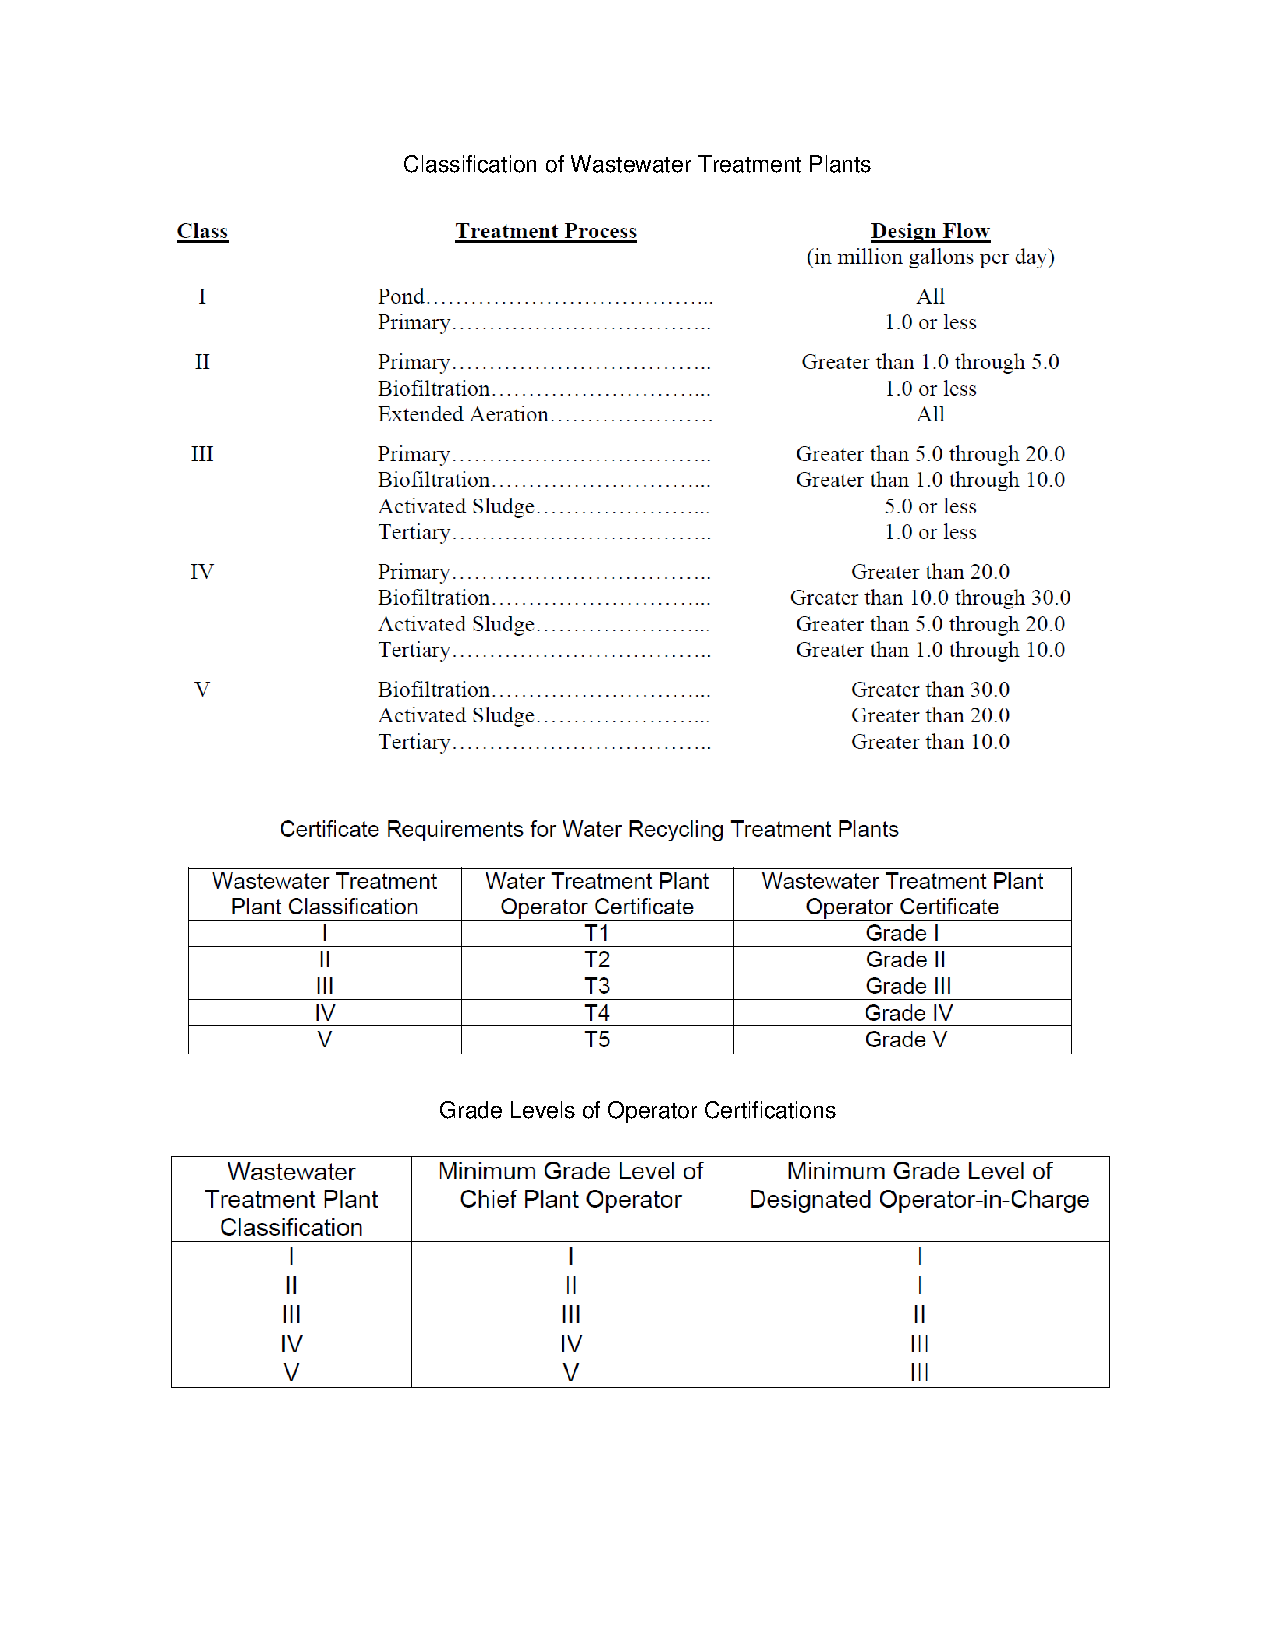
\includepdf[pages=-]{WastewaterPlantOperatorClassificationRequirements.pdf}
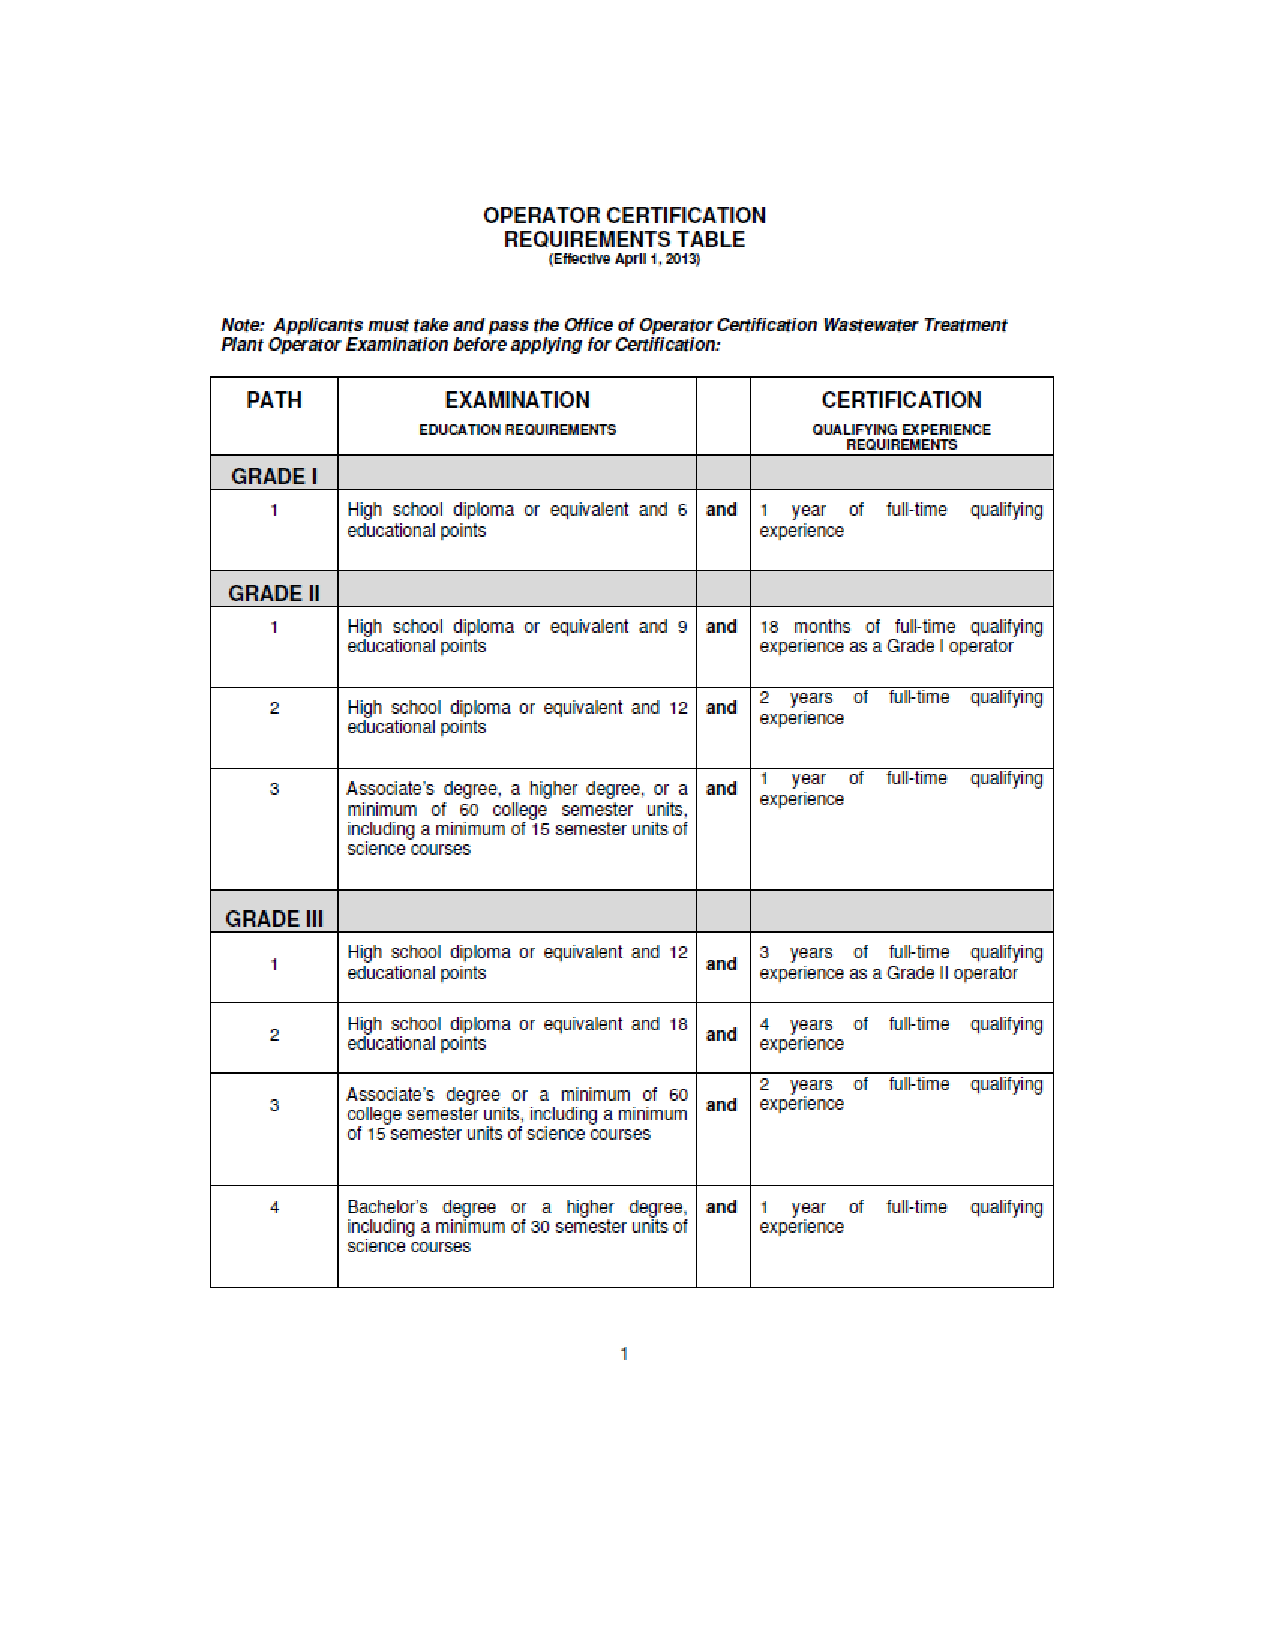
\includepdf[pages=-]{CertificationRequirement.pdf}

\subsection{Worker Safety}\index{Worker Safety}
\begin{itemize}
\item Wastewater treatment facility can be an extremely unsafe occupational field
\item It involves most of the major categories of workplace hazards:  biological, chemical, physical, safety and ergonomic,  accentuated with other factors such as shift work and diverse tasks.
\item Entities including The Occupational Safety and Health Administration(OSHA) National Electrical Code (NEC), National Fire Protection Association (NFPA), Underwriters Laboratory (UL) have recognized these hazards and implemented codes and standards to protect the affected persons and wastewater workers.
\end{itemize}

%\chapterimage{ElementsofTreatmentImg.png} % Chapter heading image
\chapter{Elements of Wastewater Treatment}

Wastewater cycle is a part of the water cycle where the water consumed as part of the normal human and industrial activity is returned back to the environment after treatment.

Wastewater cycle comprises of the following sequential elements:
\begin{enumerate}
\item Generation
\item Collection
\item Treatment
\item Disposal or reuse
\end{enumerate}

\section{Generation}\index{Generation}

Wastewater originates from domestic, industrial, commercial or agricultural activities. The characteristics of wastewater vary depending on the source. Types of wastewater include: 
\begin{itemize}
\item \hl{Domestic Sewage:}  wastewater derived principally from dwellings, business buildings, institutions, and \\
\item \hl{Industrial Sewage:}  liquid waste from industrial processes\\
\end{itemize}
Typical per person generation of wastewater in the USA is about 70-100 gallons per day

\section{Collections}\index{Collections}

\begin{itemize}
\item Wastewater is collected from its point of origin - home, businesses, industries etc. and conveyed via sewer lines to a centralized wastewater treatment facility.  
\item When the rainwater drainage is made part of the sewer system, the system is termed as \hl{Combined System}.  
\item The system where the sewage is conveyed separately from the stormwater flows is termed as \hl{Separated System}.  
\item In the Separated System, the Sanitary Sewers convey the wastewater and the Stormwater Sewer conveys the storm water flows.  
\item For the Combined System, rainstorms pose the threat of overwhelming the sewers and the treatment plant
\end{itemize}  
\begin{center}
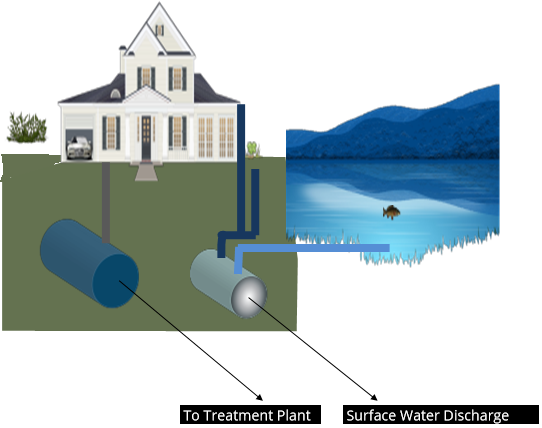
\includegraphics[scale=0.45]{SeperatedSystem1} \hspace{1 cm} 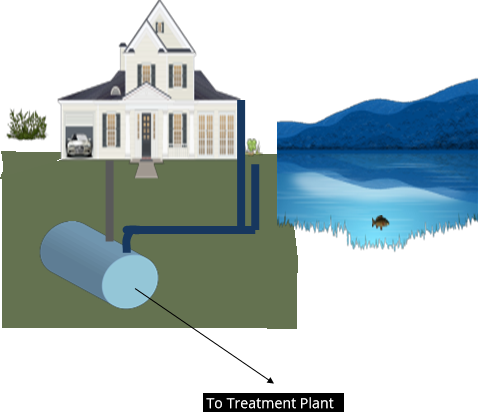
\includegraphics[scale=0.45]{CombinedSystem1}
\end{center}
			\hspace{2.6cm} Separated System \hspace{3.2cm} \parbox{\textwidth}{Combined System}\\

\section{Treatment}\index{Treatment}
\subsection{Liquid Phase Treatment}\index{Liquid Phase Treatment}
\begin{itemize}
\item Wastewater treatment can involve physical, chemical or biological processes or combinations of these processes depending on the required outflow standards. 
\item Wastewater treatment typically involves a series of steps with increasing level of treatment:
\begin{itemize}
\item \hl{Preliminary}:  The preliminary process removes large/coarse solids which include rocks, tree branches, grit and other debris present in wastewater.
\item \hl{Primary}:  The primary process is also a physical process where the separable wastewater solids - solids that float and solids that can settle, are removed.  
\item \hl{Secondary}:  Secondary treatment is a biological treatment process where microorganisms consume the organic matter present in the wastewater. 
\item \hl{Tertiary or Advanced Treatment}:  The tertiary/advanced treatment processes improve the quality of treated water beyond the secondary treatment level.  This process may include nutrient removal and disinfection.
\end{itemize}

\subsection{Treatment of Wastewater Solids}\index{Treatment of Wastewater Solids}
\begin{itemize}
\item Solids are a byproduct of wastewater treatment.  
\item Screenings and grit removed as part of the preliminary treatment is typically disposed in a landfill.
\item Sludge generated from the wastewater treatment processes -  settled solids and scum from primary and secondary treatment processes needs to be treated prior to disposal or reuse to comply with wastewater solids - biosolids regulations.
\end{itemize}

\vspace{0.5cm}
Typical solids treatment is comprised of the following three sequential steps:
\begin{enumerate}
\item Sludge thickening
\item Sludge stabilization
\item Sludge dewatering
\end{enumerate}
\vspace{0.5cm}
\subsubsection{Sludge Thickening}\index{Sludge thickening}
Sludge thickening improves performance of sludge stabilization process and provides capital and operational cost savings due to a lower volume of sludge
\subsubsection{Sludge Stabilization}\index{Sludge Stabilization}
Sludge stabilization process produces solids (biosolids) that meet Part 503 rule requirements. 
\subsubsection{Sludge Dewatering}\index{Sludge Dewatering}
Solids stabilized using digestion process has only a small percentage by weight of solids -less than 5\%.  It therefore becomes necessary to dewater the stabilized sludge prior to hauling off-site for final disposal. 
\vspace{0.5cm}
A generalized layout/process sequencing in a wastewater treatment plant is shown below:
\begin{center}
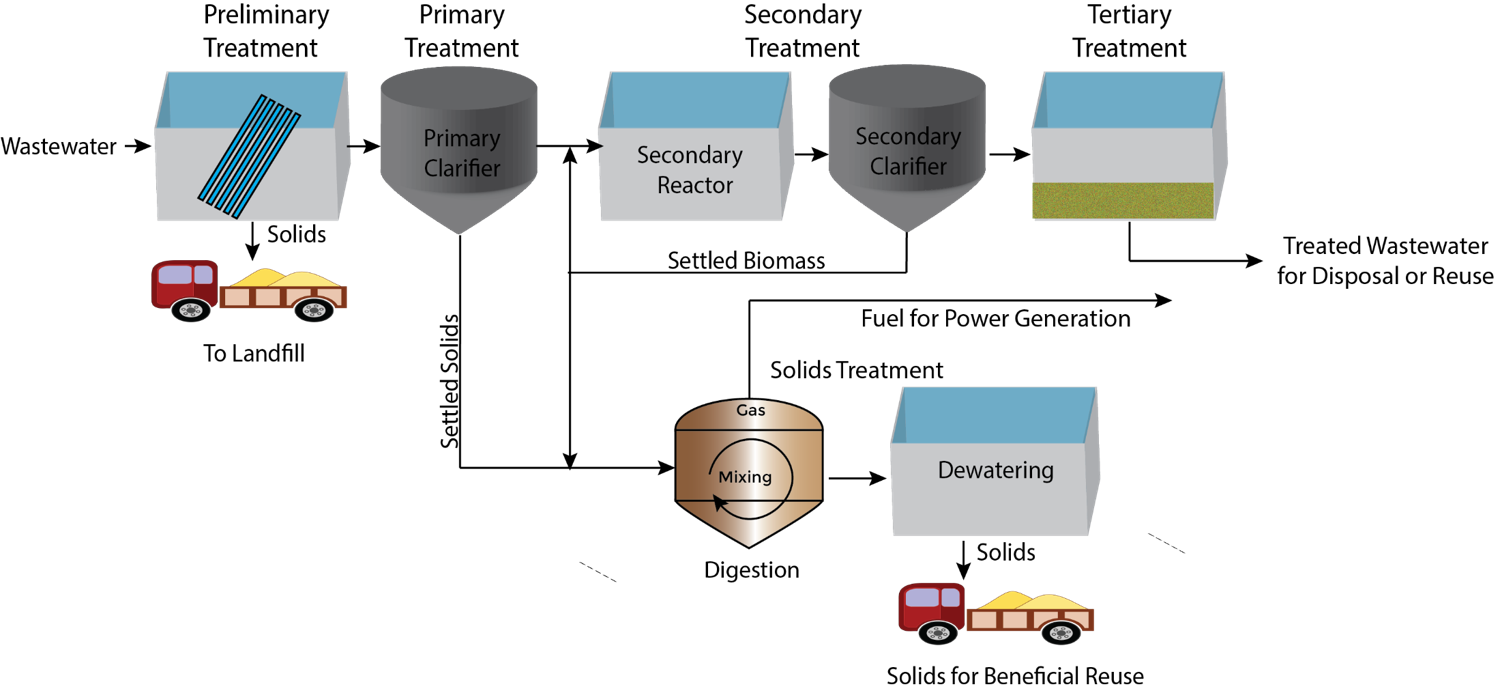
\includegraphics[scale=0.6]{TreatmentFlow}
\end{center}
Individual wastewater treatment processes involve different process options or sequences which are illustrated in the graphic below:
\begin{center}
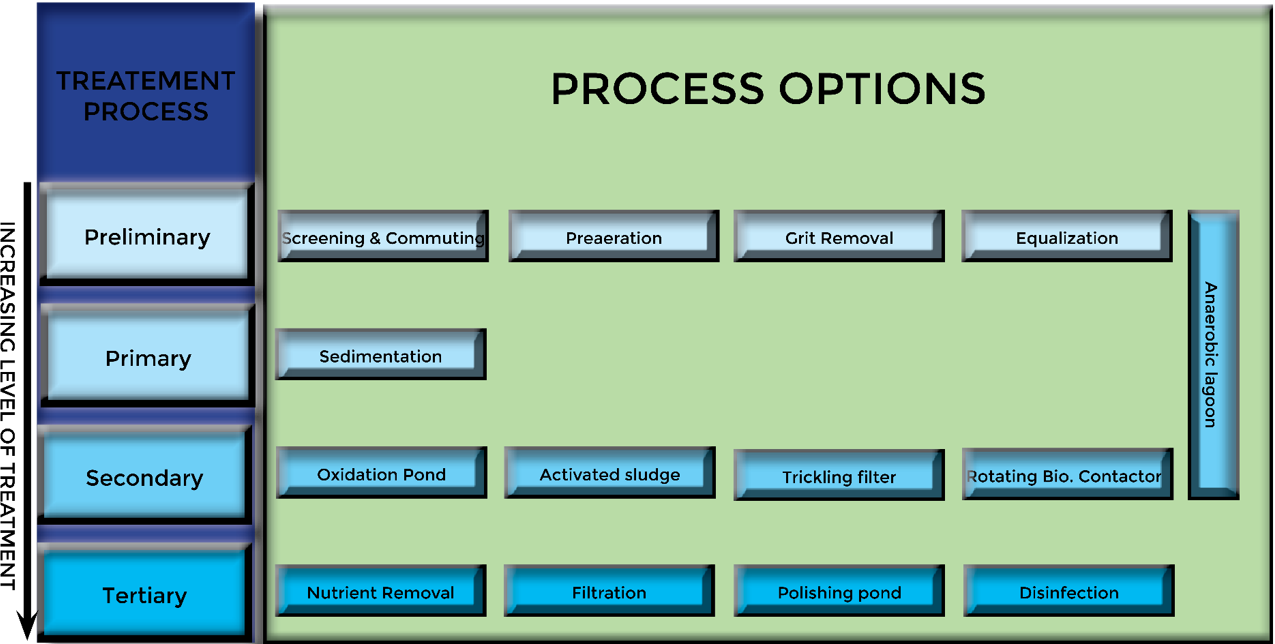
\includegraphics[scale=0.42]{Treatment}
\end{center}
\end{itemize}

\section{Disposal or Reuse}\index{Disposal or Reuse}

\begin{itemize}
\item Wastewater treatment processes can be designed to \hl{dispose} the treated water where the water is reintroduced to the environment or for \hl{reuse} where the treated water is \hl{reclaimed} or \hl{recycled} - for various purposes including irrigation, industrial use or for potable use.
\item Water disposal methods include:\\
\begin{itemize}
\item \hl{Surface water discharge}
\item \hl{Subsurface discharge}
\end{itemize}
\item Water reuse methods include:\\
\begin{itemize}
\item Potable water reuse
\begin{itemize}
\item \hl{Indirect potable reuse:}  Here the treated water is blended with groundwater or surface water and then reclaimed and treated further 
for drinking (potable) water use
\item \hl{Direct potable reuse:}  Here the treated wastewater is subjected to advanced treatment and introduced directly into a municipal water supply system
\end{itemize}
\item Water reclamation for irrigation or industrial use\\
\item Land application for beneficial use\\
\end{itemize}
\item Solids generated from the wastewater treatment process may be removed and disposed to a landfill or subject to further treatment which may allow for energy recovery - from the organic solids and for beneficial reuse due to its plant nutrient content.\\
\end{itemize}


\part{Week 1}
\chapterimage{MathCover.png}
\chapter{Water Math - Week 3}

\section*{Density}\index{Density}
\begin{itemize}
\item Density is defined as the weight of a substance per a unit of its volume. For example, pounds per cubic foot or pounds per gallon.

\item Here are a few key facts about density:
\begin{itemize}

\item Density is measured in units of lb/ft3, lb/gal, or mg/L. Density of water = 62.4 lb/ft3 = 8.34 lb/gal.
\end{itemize}
\end{itemize}

\section*{Specific Gravity}\index{Specific Gravity}
\begin{itemize}
\item Specific gravity is the ratio of the density of a substance (liquid or solid) to the density water.
\item It is the ratio of the weight of the substance of a certain volume to the weight of water of the same volume.

\item Any substance with a density greater than that of water will have a specific gravity greater than 1.0. Any substance with a density less than that of water will have a specific gravity less than 1.0. 

\item Specific gravity examples:
\begin{itemize}

\item Specific gravity of water = 1.0 
\item Specific gravity of concrete = 2.5 (depending on ingredients)
\item Specific gravity of alum (liquid @ 60°F) = 1.33 
\item Specific gravity of hydrogen peroxide (35\%) = 1.132
\end{itemize}

\item Specific gravity is used in two ways:
\begin{enumerate}
\item To calculate the total weight of a \% solution (either as a single gallon or a drum volume).\\
Total Weight = Drum Vol X SG X 8.34
\item To calculate the “active ingredient” weight of a single gallon or a drum.\\

Active Ingredient Weight within Drum = Drum Volume X SG X 8.34 X \% solution as a decimal. (i.e., Total Weight X \% solution as a decimal)\\

NOTE: Both ways start with solving for the total weight (Drum Vol X SG X 8.34). When solving for “active ingredient” weight, you have to then multiply by \% solution as a decimal.

\end{enumerate}
\end{itemize}

\textbf{Example:} What is the weight of 5 gallons of a 40\% ferric chloride solution given its specific gravity of 1.43?
$$(8.34 * 1.43) \enspace lbs/gal*5 \enspace gallons = \boxed{59.6 \enspace lbs}$$

The weight of active ferric chloride in the drum will be 59.6*0.4=23.84 lbs (as ferric chloride is 40\% strength)

% \begin{tcolorbox}[
% colframe=blue!25,
% colback=blue!10,
% coltitle=blue!20!black,  
% title= Practice Problems]
% \begin{enumerate}
% \item What is the specific gravity of a 1 ft$^3$ concrete block which weighs 145 lbs?

% \item What is the specific gravity of a chlorine solution if 1 (one) gallon weighs 10.2lbs?

% \item How much does each gallon of zinc orthophosphate weigh (pounds) if it has a specific gravity of 1.46?

% \item How much does a 55 gallon drum of 25\% caustic soda weigh (pounds) if the specific gravity is 1.28?

% \end{enumerate}

% \end{tcolorbox}


\section*{Concentration}\index{Concentration}
\begin{itemize}
\item Concentration is typically expressed as mg/l which is the weight of the constituent (mg) in 1 liter of water.
\item As 1 liter of water weighs 1 million mg, a concentration of 1 mg/l implies 1 mg of constituent per 1 million mg of water or one part per million (ppm).   \texthl{Thus, mg/l and ppm are synonymous.}
\item Sometimes the constituent concentration is expressed in terms of percentage.\\
\vspace{6pt}
\textbf{Example:} 12.5\% chlorine concentration solution.\\
\vspace{0.2cm}
100\% would mean 1,000,000 mg/l or 1,000,000 ppm\\
\vspace{0.2cm}
$\implies$1\% would be $\dfrac{1,000,000}{100}\textrm{mg/l} = \textrm{10,000 mg/l or 10,000 ppm}$\\
\vspace{0.2cm}
$\implies$12.5\% chlorine concentration is 125,000 mg/l or 125,000 ppm.
\vspace{6pt}

$1\% \enspace concentration = 10,000 \enspace ppm \enspace or \enspace\dfrac{mg}{l}$\\
$0.1\% \enspace concentration = 1,000 \enspace ppm \enspace or \enspace \dfrac{mg}{l}$\\
$0.01\% \enspace concentration = 100 \enspace ppm \enspace or \enspace \dfrac{mg}{l}$\\
$10\% \enspace concentration = 100,000 \enspace ppm \enspace or \enspace \dfrac{mg}{l}$\\
$5\% \enspace concentration = 50,000 \enspace ppm \enspace or \enspace \dfrac{mg}{l}$\\
$12.5\% \enspace concentration = 125,000 \enspace ppm \enspace or \enspace \dfrac{mg}{l}$\\
\end{itemize}

\vspace{0.3cm}
Above concepts are used for chemicals such as fluoride and hypochlorites - the strength of the product as used is commonly expressed as a percentage.
\vspace{0.3cm}

\textbf{Example 1:} A chlorine solution was made to have a $4 \%$ concentration. It is often desirable to determine this concentration in $\mathrm{mg} / \mathrm{L}$. This is relatively simple: the $4 \%$ is four percent of a million.

To find the concentration in $\mathrm{mg} / \mathrm{L}$ when it is expressed in percent, do the following:

\begin{enumerate}
  \item Change the percent to a decimal.
\end{enumerate}
$$
4 \% \div 100=0.04
$$

\begin{enumerate}
  \setcounter{enumi}{2}
  \item Multiply times a million.
\end{enumerate}
$$
0.04 \times 1,000,000=40,000 \mathrm{mg} / \mathrm{L}
$$
We get the million because a liter of water weighs $1,000,000 \mathrm{mg} .1 \mathrm{mg}$ in 1 liter is 1 part in a million parts ( $\mathrm{ppm}) .1 \%=10,000 \mathrm{mg} / \mathrm{L}$.


\textbf{Example 2:} How much $65 \%$ calcium hypochlorite is required to obtain 7 pounds of pure chlorine?\\
$65 \%$ implies that in every lb of calcium hypochlorite has $65 \%$ lbs of available chlorine.\\
\vspace{0.2cm}
Therefore, $\dfrac{0.65 \textrm{ lbs available chlorine}}{\textrm{lb of calcium hypochlorite}} $ or conversely $\dfrac{\textrm{lb of calcium hypochlorite}}{0.65 \textrm{ lbs available chlorine}}$\\
\vspace{0.2cm}
$\implies{\textrm{lbs calcium hypchlorite required}}=\dfrac{\textrm{lb of calcium hypochlorite}}{0.65 \cancel{\textrm{ lbs available chlorine}}}*\dfrac{7\cancel{\textrm{ lb of available chlorine}}}{}$\\
\vspace{0.2cm}
$=\boxed{10.8 \textrm{ lbs of calcium hypochlorite with } 65\%\textrm{available chlorine is required}}$

% \begin{tcolorbox}[
% colframe=blue!25,
% colback=blue!10,
% coltitle=blue!20!black,  
% title= Practice Problems]
% \begin{enumerate}
% \item What is the concentration in mg/l of  4.5\% solution of that substance.
% \item How many lbs of salt is needed to make 5 gallons of a 2,500mg/l solution
% \end{enumerate}
% \end{tcolorbox}


\section*{Pounds Formula}\index{Pounds Formula}
\begin{itemize}
\item Pounds formula: 
$$lbs \enspace \textbf{or} \enspace \dfrac{lbs}{day}=Concentration\Big(\dfrac{mg}{l}\Big)*8.34*volume(MG) \enspace \textbf{or} \enspace Flow (MGD)$$\\
\item So if the concentration of a particular constituent (in mg/liter) and the volume or flow of wastewater is given, one can calculate the amount of that constituent or using this formula.\\
\texthl{Important notes:}\\
\begin{enumerate}
\item \texthl{The unit of the constituent loading rate will be in lbs per the unit of time the flow is expressed in.  So if the flow is in MG per day the calculated loading rate will be in lbs/day.  Likewise if the flow value used is in MG per minute, the calculated loading rate will be in lbs/min.}
\item \texthl{If volume is used, the calculated value will be the mass of the constituent in that volume.  If flow is used, the calculated value will be the mass of the constituent in that flow.}
\item \texthl{For the Pound Formula to work, the volume or flow needs to be expressed in MG.  Volume or flows in other units - gallons, $ft^3$ etc. needs to be converted to MG.}
\end{enumerate}

\item The formula assumes that all of the material found in water (TSS, BOD, MLSS, Chlorine, etc.) weighs the same as water, that is, $8.34$ pounds per gallon.
\item In the Pounds Formula, there are three variables – lbs, concentration and volume, and one constant - 8.34.  Knowing any of the two variables in the formula, one can calculate the third (unknown) variable by rearranging the equation.\\
\begin{figure}[h]
\begin{tikzpicture}
    \newcommand{\R}{3}

\path[help lines,step=.2] (0,0) grid (16,6);
\path[help lines,line width=.6pt,step=1] (0,0) grid (16,6);
%\foreach \x in {0,1,2,3,4,5,6,7,8,9,10,11,12,13,14,15,16}
%\node[anchor=north] at (\x,0) {\x};
%\foreach \y in {0,1,2,3,4,5,6}
%\node[anchor=east] at (0,\y) {\y};
%-------------CIRCLE-----------------------------------
\draw[black,fill=gray!10] (8,3) circle (\R);
\draw[black, very thick, rotate=0](5,3) -- (11,3);
\draw (8,4.5) node[text width=3cm,align=center]
  {\scriptsize{lbs or lbs/day}};
\draw (6.4,2) node[text width=3cm,align=center]
  {\scriptsize{Concentration\\mg/l}};
\draw (9.7,2) node[text width=3cm,align=center]
  {\scriptsize{Volume(MG)\\Flow(MGD)}};
  \draw (8,1)node[text width=3cm,align=center]
  {\scriptsize{8.34}};
\draw[black, very thick, rotate=0](6.4,0.5) -- (8,3);
\draw[black, very thick, rotate=0](9.6,0.5) -- (8,3);
  \node [circle split,draw,double,fill=red!20] at (4,3)
  {
    % No \nodepart has been used, yet. So, the following is put in the
    % ``text'' node part by default.
    $\div$
    \nodepart{lower} % Ok, end ``text'' part, start ``output'' part
    $=$
  };
  
    \node [circle split,draw,double,fill=red!20] at (5.8,-0.2)
  {
    % No \nodepart has been used, yet. So, the following is put in the
    % ``text'' node part by default.
    \scriptsize{$X$}
    \nodepart{lower} % Ok, end ``text'' part, start ``output'' part
    \tiny{$Multiply$}
  };
  
    \node [circle split,draw,double,fill=red!20] at (10,-0.2)
  {
    % No \nodepart has been used, yet. So, the following is put in the
    % ``text'' node part by default.
    \scriptsize{$X$}
    \nodepart{lower} % Ok, end ``text'' part, start ``output'' part
    \tiny{$Multiply$}
  };
\end{tikzpicture}
\caption{Davidson Pie}
\end{figure}
\vspace{0.2cm}
\item Davidson Pie provides a pictorial reference for calculating any unknown variable.  If for example, if Concentration is unknown, it can be calculated as follows: \\$$Concentration\Big(\dfrac{mg}{l}\Big)=\dfrac{lbs \enspace \textbf{or} \enspace \dfrac{lbs}{day}}{8.34*Volume(MG) \enspace \textbf{or} \enspace Flow (MGD)}$$\\
\vspace{0.2cm}
\item Likewise, if Volume (or Flow) is the unknown variable. it can be calculated as:  \\$$Volume (MG) \enspace or \enspace Flow(MGD)=\dfrac{lbs \enspace \textbf{or} \enspace \dfrac{lbs}{day}}{Concentration\Big(\dfrac{mg}{l}\Big)* \enspace 8.34  }$$
\vspace{0.2cm}
\item Pounds formula is used for:
\begin{itemize}
\item Calculating the quantity in pounds of a particular wastewater constituent entering or leaving a wastewater treatment process
\item Calculating the pounds of chemicals to be added\\
\end{itemize}
\end{itemize}
\section*{Forms of chlorine}\index{Forms of chlorine}

\begin{itemize}
	\item Due to safety issues related to the use of chlorine gas, \textbf{hypochlorites} are often used in lieu of chlorine
	\item Types of hypochlorites
	\begin{itemize}
	\item Sodium hypochlorite (NaOCl) comes in a liquid form which contains up to 12.5\% chlorine
	\item Calcium hypochlorite (Ca(OCl)$_2$), also known as High-test Hypochlorite (HTH), is a solid which is mixed with water to form a hypochlorite solution. Calcium hypochlorite is 65-70\% concentrated.
	\end{itemize}
	\item Hypochlorites decompose in strength over time while in storage. Temperature, light, and physical energy can all break down hypochlorites before they are able to react with pathogens in water. 

\end{itemize} 
\subsection*{Chlorine dosing terms}\index{Chlorine dosing terms}
\begin{itemize}
\item \textbf{Chlorine dose} - the amount of chlorine added to the system. It can be determined by adding the desired residual for the finished water to the chlorine demand of the untreated water. Dosage can be either milligrams per liter (mg/L) or pounds per day (lb/day).

\item \textbf{Chlorine Demand} - the amount of chlorine consumed by iron, manganese, turbidity, algae, and microorganisms in the water. Because the reaction between chlorine and microorganisms is not instantaneous, demand is relative to time. For instance, the demand 5 minutes after applying chlorine will be less than the demand after 20 minutes. 

\item \textbf{Free chlorine} - free chlorine refers to all chlorine present in the water as Cl$_2$(g), HOCl(aq) and OCl$^-$(aq).

\item \textbf{Combined residual} - is the result of combining free chlorine with nitrogen compounds. Combined residuals are also referred to as chloramines. 

\item \textbf{Total chlorine residual} - is the mathematical combination of free chlorine and combined residuals. Total residual can be determined directly with standard chlorine residual test kits.  Residual, like demand, is based on time. The longer the time after dosage, the lower the residual will be, until all of the demand has been satisfied. Residual, like demand, is expressed in $\mathrm{mg} / \mathrm{L}$. The presence of a free residual usually provides a high degree of assurance that the disinfection of the water is complete. 

$$\mathrm{Chlorine Dose} (\mathrm{mg} / \mathrm{L})= \mathrm{Chlorine Demand}+ \mathrm{ Chlorine Residual}$$
\end{itemize}
\textbf{Example 1:} If a 5 MGD flow is to be dosed with 25 mg/l of a certain chemical, calculate the lbs/day that chemical required.\\

Solution\\

Applying lbs formula:\\
$\dfrac{lbs}{day}=5 MGD *250\dfrac{mg}{l}*8.34 = \boxed{1,042\dfrac{lbs}{day}}$
\\
\vspace{6pt}
\textbf{Example 2:} Calculate the lbs of chemical in 7,500 gallons of 4.5\% active solution of that chemical.\\
Solution\\
Applying lbs formula:\\
$lbs chemical = \dfrac{7500}{1,000,000}MG * 4.5*10,000 *8.34 = \boxed{2,815 \enspace lbs \enspace chemical}$\\
\textbf{Note:}\\  
1) 7500 gallons was converted to MG by dividing by 1,000,000\\
$7500 \enspace gallons * \dfrac{1 MG}{1,000,000 \enspace gallon}$\\
2) 4.5\% was converted to mg/l by multiplying by 10,000 as 1\%=10,000mg/l

% \begin{tcolorbox}[
% colframe=blue!25,
% colback=blue!10,
% coltitle=blue!20!black,  
% title= Practice Problems]

% \begin{enumerate}

% \item A water treatment plant operates at the rate of 75 gallons per minute. They dose soda ash at
% 14 mg/L. How many pounds of soda ash will they use in a day?

% \item A water treatment plant is producing 1.5 million gallons per day of potable water, and
% uses 38 pounds of soda ash for pH adjustment. What is the dose of soda ash at that plant?

% \item A water treatment plant produces 150,000 gallons of water every day. It uses an
% average of 2 pounds of permanganate for iron and manganese removal. What is the dose of the
% permanganate? 

% \item A water treatment plant uses 8 pounds of chlorine daily and the dose is 17 mg/l. How
% many gallons are they producing?

% \item An operator mixes 40 lb of lime in a 100-gal tank containing 80 gal of water. What is the percent of lime in the slurry?

% \end{enumerate}
% \end{tcolorbox}

\section*{Chemicals Related Math Problems}\index{Chemicals Related Math Problems}
\subsection*{Chemical Dosing}\index{Chemical Dosing}

\begin{itemize}
\item Use lbs formula to calculate the lbs of chemicals required\\
\item Using the calculated lbs chemical required value, calculate the amount of that chemical at the concentration available
\end{itemize}

\textbf{Example 1:} If a 5 MGD flow is to be dosed with 25 mg/l of a certain chemical, calculate the lbs/day that chemical required.\\

Solution\\

Applying lbs formula:\\
$\dfrac{lbs}{day}=5 MGD *250\dfrac{mg}{l}*8.34 = \boxed{1,042\dfrac{lbs}{day}}$
\\
\vspace{6pt}
\textbf{Example 2:} Calculate the lbs of chemical in 7,500 gallons of 4.5\% active solution of that chemical.\\
Solution\\
Applying lbs formula:\\
$lbs chemical = \dfrac{7500}{1,000,000}MG * 4.5*10,000 *8.34 = \boxed{2,815 \enspace lbs \enspace chemical}$\\

\subsection*{Chlorine dosing problems}\index{Chlorine dosing problems}
\textbf{Example 4:} Determine the chlorinator setting (lb/day) required to treat a flow of $4 \mathrm{MGD}$ with a chlorine dose of $5 \mathrm{mg} / \mathrm{L}$.

Chlorine feed rate $(\mathrm{lb} /$ day $)=$ Chlorine $(\mathrm{mg} / \mathrm{L}) \times$ Flow $(\mathrm{MGD}) \times 8.34 \mathrm{lb} / \mathrm{gal}$

Chlorine feed rate $(\mathrm{lb} /$ day $)=5 \mathrm{mg} / \mathrm{L} \times 4 \mathrm{MGD} \times 8.34 \mathrm{lb} / \mathrm{gal}$

Chlorine feed rate $(\mathrm{lb} /$ day $)=167 \mathrm{lb} /$ day

\textbf{Example 5:} A pipeline that is 12 inches in diameter and $1400 \mathrm{ft}$ long is to be treated with a chlorine dose of $48 \mathrm{mg} / \mathrm{L}$. How many lb of chlorine will this require?

First determine the gallon volume of the pipeline:

Volume $(\mathrm{gal})=0.785 \times \mathrm{D}^{2} \times$ length $(\mathrm{ft}) \times 7.48 \mathrm{gal} / \mathrm{cu} \mathrm{ft}$

Volume $(\mathrm{gal})=0.785 \times(1 \mathrm{ft})^{2} \times 1400 \mathrm{ft} \times 7.48 \mathrm{gal} / \mathrm{cu} \mathrm{ft}$ Volume $(\mathrm{gal})=8221 \mathrm{gal}$

Next calculate the amount of chlorine required:

Chlorine feed rate $(\mathrm{lb} /$ day $)=$ Chlorine $(\mathrm{mg} / \mathrm{L})$ x Flow $($ MGD) $\times 8.34 \mathrm{lb} / \mathrm{gal}$

Chlorine feed rate $(\mathrm{lb} /$ day $)=48 \mathrm{mg} / \mathrm{L} \times 0.008221 \mathrm{MGD} \times 8.34 \mathrm{lb} / \mathrm{gal}$

Chlorine feed rate $(\mathrm{lb} /$ day $)=3.3 \mathrm{lb}$

\textbf{Example 6:} A water sample is tested and found to have a chlorine demand of $1.7 \mathrm{mg} / \mathrm{L}$. If the desired chlorine residual is $0.9 \mathrm{mg} / \mathrm{L}$, what is the desired chlorine dose (in $\mathrm{mg} / \mathrm{L}$ )?

Chlorine Dose $(\mathrm{mg} / \mathrm{L})=$ Chlorine Demand $+$ Chlorine Residual

Chlorine Dose $(\mathrm{mg} / \mathrm{L})=1.7 \mathrm{mg} / \mathrm{L}+0.9 \mathrm{mg} / \mathrm{L}$

Chlorine $\operatorname{Dose}(\mathrm{mg} / \mathrm{L})=2.6 \mathrm{mg} / \mathrm{L}$

\textbf{Example 7:}\\
The chlorine dosage for water is $2.7 \mathrm{mg} / \mathrm{L}$. If the chlorine residual after a 30-minute contact time is found to be $0.7 \mathrm{mg} / \mathrm{L}$, what is the chlorine demand (in $\mathrm{mg} / \mathrm{L}$ )?

Chlorine Demand $=$ Chlorine Dose $-$ Chlorine Residual

Chlorine Demand $=2.7 \mathrm{mg} / \mathrm{L}-0.7 \mathrm{mg} / \mathrm{L}$

Chlorine Demand $=2.0 \mathrm{mg} / \mathrm{L}$

\textbf{Example 8:} How many gallons per day of bleach solution (SG 1.2)containing 12.5\% available chlorine is required to disinfect a 10 MGD flow of water given the required chlorine dosage of 7 mg/l.\\
\begin{enumerate}
\item Calculate the lbs of chlorine required using the lbs formula:\\
\vspace{0.5cm}
=$10 MGD \enspace * \enspace 7 \dfrac{mg}{l} \enspace * \enspace 8.34\enspace=\enspace 583.8 \enspace lbs \enspace chlorine \enspace per \enspace day$\\
\vspace{0.5cm}
\item Calculate the gallons of bleach which will provide the 583.8 lbs chlorine\\
\vspace{0.5cm}
Applying the lbs formula - note that 8.34 * SG will give the actual lbs/gal of bleach.  If SG is not provided, use only 8.34 lbs per gallon:\\
\vspace{0.5cm}
$583.8 \dfrac{lbs \enspace bleach}{day}\enspace=\enspace x \dfrac{gal}{day} \enspace * \enspace 8.34 * 1.2 \dfrac{lbs \enspace bleach}{gal} \enspace * \enspace 0.0125 \dfrac{lbs \enspace chlorine}{lb \enspace bleach} \enspace $\\
\vspace{0.5cm}
$ \implies x \dfrac{gal}{day}\enspace = \enspace \dfrac{583.8}{8.34*1.2*0.125} \enspace = \boxed{467 \dfrac{gal}{day}}$
\end{enumerate}
\vspace{0.3cm}
\textbf{The above problem can be solved directly using the formula below given in the SWRCB Water Treatment Exam Formula Sheet.}\\
\vspace{0.3cm}
 $\textrm{GPD}=\dfrac{\textrm{(MGD)}*\textrm{(ppm or mg/l)}*8.34 \enspace \textrm{lbs/gal}}{\textrm{\% \enspace purity}*\textrm{Chemical \enspace Wt. (lbs/gal)}}$ 
 \vspace{0.3cm}
 $\textrm{GPD}=\dfrac{10*7*8.34}{0.125*(1.2*8.34)}=\boxed{467 \dfrac{\textrm{gal}}{\textrm{day}}}$ 

% \begin{tcolorbox}[
% colframe=blue!25,
% colback=blue!10,
% coltitle=blue!20!black,  
% title= Practice Problems]
% \begin{enumerate}

%   \item Determine the chlorinator setting in pounds per day if a water plant produces $300 \mathrm{gpm}$ and the desired chlorine dose is $2.0 \mathrm{mg} / \mathrm{L}$.

%   \item The finished water chlorine demand is $1.2 \mathrm{mg} / \mathrm{L}$ and the target residual is $2.0 \mathrm{mg} / \mathrm{L}$. If the plant flow is $5.6 \mathrm{mgd}$, how many pounds per day of $65 \%$ hypochlorite solution will be required?

%   \item Fluoride is added to finished water at a dose of $4 \mathrm{mg} / \mathrm{L}$. Find the feed rate setting for a fluoride saturator in gal/min if the water plant produces $5 \mathrm{mgd}$.

%   \item If chlorine costs $\$ 0.21$ per pound, what is the daily cost to chlorinate a $5 \mathrm{mgd}$ flow rate at a dosage of $2.6 \mathrm{mg} / \mathrm{L}$ ?

%   \item One gallon of sodium hypochlorite laundry bleach, with $5.25 \%$ available chlorine, contains how many pounds of active chlorine?


% \end{enumerate}
% \end{tcolorbox}


\subsection*{Blending and Dilution Calculations}\index{Blending and Dilution Calculations}
\begin{itemize}
\item Blending and dilution calculations apply to the following scenarios:
\begin{itemize}
\item Blending involves mixing two streams - each with a different concentration of contaminant/chemical, to obtain a certain volume or flow containing the target concentration of contaminant/chemical.  For example: \textit{Finding the correct blend of two source water streams - one with 15 mg/L of iron and other containing  4 mg/L of iron to get a 100 gpm product water containing 8 mg/l of iron.} \textbf{OR}\\
\textit{Calculating the actual combined TDS concentration obtained by mixing two known flows with known TDS concentrations.}
\item Dilution involves makedown of a higher concentration of a chemical to a lower concentration using water as a dilutant.   For example: \textit{How much initial volume of a 4\% polymer solution is needed to make 3500 gallons of polymer at 0.25\% concentration?}\\
\end{itemize}
\item These type of problems are solved using C*V relationship where:
\begin{itemize}
 \item C is the concentration expressed in ppm or mg/l or as \% purity.
 \item V is either the volume or flow.
\item The product - C*V - $\dfrac{\textrm{\textrm{mass}}}{\textrm{volume}/\textrm{flow}}*\textrm{volume/flow} = \textrm{mass}$  
\end{itemize}
\item For blended streams, the sum of the mass from each of the two source streams will equal to the mass in the target stream:

\item Thus, \textbf{for blending calculations}, if:\\

C$_1$ and V$_1$ is the concentration and volume respectively of the one of the sources streams and\\
\vspace{0.2cm}
 C$_2$ and V$_2$ is the concentration and volume respectively of the second source stream, and \\
 \vspace{0.2cm}
C$_3$ and and V$_3$ is the concentration and volume respectively of the target stream\\
\vspace{0.3cm}
The sum of the mass from each of the two source streams will equal to the mass in the target stream:\\
\vspace{0.3cm}
\textbf{C$_1$ * V$_1$ + C$_2$ * V$_2$ =  C$_3$ * V$_3$.}\\
\vspace{0.3cm}
This equation can be manipulated algebraically to calculate anyone of the unknown values in the equation.\\
\vspace{0.2cm}
Also, any of the three volume variables can be expressed as the sum or difference of the other two - , or V$_1$ + V$_2$ = V$_3$ or V$_1$ = V$_3$ - V$_2$ or V$_2$ = V$_T$ - V$_1$\\

\item \textbf{For dilution}, the mass of the target chemical will remain the same, as only water is added to the source (concentrated chemical).
\item Thus, for dilution calculations, if:\\
\vspace{0.2cm}
C$_1$ and V$_1$ is the concentration and volume respectively of the concentrated product used for the dilution, and\\
\vspace{0.2cm}
C$_2$ and V$_2$ is the concentration and volume of the resultant product after dilution with water\\
\vspace{0.2cm}
The mass of the target chemical in the volume of the concentrated product used for dilution will remain the same in the final diluted product:\\
\vspace{0.3cm}
\textbf{C$_1$ * V$_1$ =  C$_2$ * V$_2$.}\\

\end{itemize}

\textbf{Example Problem \#1:} Two wells are used to satisfy demand during the summer months. One well produces water that contains 22 mg/L of Arsenic. The other well produces water that contains 3 mg/L of Arsenic. If the total demand for water is 400 gpm and the target Arsenic concentration in the finished water is 8 mg/L, what is the highest pumping rate possible for the first well?\\
\vspace{0.3cm}
\textbf{Solution:}\\
C$_1$ * V$_1$ + C$_2$ * V$_2$ =  C$_3$ * V$_3$\\
\vspace{0.3cm}
Thus 22 * V$_{22}$ + 3 * V$_3$ =  8 * V$_8$\\
\vspace{0.3cm}

V$_{22}$ + V$_3$ = V$_8$ = 400 gpm\\
\vspace{0.3cm}
As we want to solve for V$_{22}$, we can express V$_3$ as: V$_3$ = 400-V$_{22}$\\
\vspace{0.3cm}
Thus, 22 * V$_{22}$ + 3 * (400-V$_{22}$) =  8 * 400=3,200\\
\vspace{0.3cm}
22V$_{22}$ + 1200-3V$_{22}$ =  3,200\\
\vspace{0.3cm}
V$_{22}$(22-3) =  2,000\\
\vspace{0.3cm}
V$_{22}$ = $ \dfrac{2,000}{19}=\boxed{105.3 \enspace gpm}$\\
\vspace{0.3cm}
Also, V$_3$=400-105.3=294.7\\
\vspace{0.3cm}

NOTE:  If one does not want to utilize algebraic manipulation, one may memorize the following formula:\\
\vspace{0.3cm}
$V_{1/2}=\dfrac{\lvert C_3 - C_{2/1}\rvert*V_3}{C_1-C_2}$\\
\vspace{0.3cm}
Applying the formula above to Example Problem \#2:\\
\vspace{0.3cm}
$V_{22}=\dfrac{\lvert 8 - 3\rvert*400}{22-3}=\boxed{105.3 \enspace gpm}$\\
\vspace{0.3cm}
$V_{3}=\dfrac{\lvert 8 - 22\rvert*400}{22-3}=\boxed{294.7 \enspace gpm}$\\
\vspace{0.3cm}
\textbf{Example Problem \#2:}  How many gallons of a 4\% polymer solution is required to make a 3,500 gallon batch of 0.25\% polymer solution.\\

\textbf{Solution:}\\
\vspace{0.3cm}
Here, we are adding water - which has zero percent of polymer concentration to the 4\% polymer to make a 0.25\% polymer solution.\\
\vspace{0.3cm}
C$_1$ * V$_1$ = C$_2$ * V$_2$\\
\vspace{0.3cm}
C$_{4\%}$ * V$_{4\%}$ =  C$_{0.25\%}$ * V$_{0.25\%}$\\
\vspace{0.3cm}
4 * V$_{4\%}$ =  0.25 * 3,500\\
\vspace{0.3cm}
$\implies V_{4\%} = \dfrac{0.25 \enspace * \enspace 3500}{4}= \boxed{219 \enspace\textrm{gal}} $\\
\vspace{0.3cm}
Take 219 gallons of the 4\% polymer and dilute to 3,500 gallons to give a 0.25\% polymer solution.\\

\section*{Disinfection Math Problems}
\begin{enumerate}
\item What is the concentration in mg/l of  4.5\% solution of that substance.\\
\vspace{0.2cm}
Solution:\\
\vspace{0.2cm}
$\boxed{45,000mg/l}$

\item How much does each gallon of zinc orthophosphate weigh (pounds) if it has a specific gravity of 1.46?\\
\vspace{0.2cm}
Solution:\\
\vspace{0.2cm}
$8.34\dfrac{lb}{gal}*1.46=\boxed{12.18\dfrac{lb}{gal}}$
\vspace{0.2cm}
\item How much does a 55 gallon drum of 25\% caustic soda weigh (pounds) if the specific gravity is 1.28?\\
\vspace{0.2cm}
Solution:\\
\vspace{0.2cm}
$8.34\dfrac{lb}{\cancel{gal}}*1.28*55\cancel{gal}=\boxed{12.18\dfrac{lb}{gal}}$
\vspace{0.2cm}
\item A water treatment plant operates at the rate of 75 gallons per minute. They dose soda ash at 14 mg/L. How many pounds of soda ash will they use in a day?
Solution:\\
\vspace{0.2cm}
\begin{figure}[h]
\begin{tikzpicture}
    \newcommand{\R}{1.5}

\path[help lines,step=.2] (0,0) grid (16,3);
\path[help lines,line width=.6pt,step=1] (0,0) grid (16,3);
%\foreach \x in {0,1,2,3,4,5,6,7,8,9,10,11,12,13,14,15,16}
%\node[anchor=north] at (\x,0) {\x};
%\foreach \y in {0,1,2,3,4,5,6}
%\node[anchor=east] at (0,\y) {\y};
%-------------CIRCLE-----------------------------------
\draw[black,fill=gray!10] (8,3) circle (\R);
\draw[black, very thick, rotate=0](6.5,3) -- (9.5,3);
\draw (8,3.6) node[text width=3cm,align=center]
  {\scriptsize{lbs/day}};
\draw (7.1,2.5) node[text width=3cm,align=center]
  {\tiny{14 mg/l}};
\draw (8.9,2.5) node[text width=3cm,align=center]
  {\tiny{75 GPM}};
  \draw (8,2)node[text width=3cm,align=center]
  {\tiny{8.34}};
\draw[black, very thick, rotate=0](7.2,1.7) -- (8,3);
\draw[black, very thick, rotate=0](8.8,1.7) -- (8,3);
\end{tikzpicture}
\end{figure}
$\dfrac{\mathrm{lbs}}{\mathrm{day}}=\mathrm{Flow}\dfrac{{\mathrm{MG}}}{\mathrm{day}}* \mathrm{Concentration}\dfrac{\mathrm{mg}}{\mathrm{l}}*8.34$
\\
\vspace{0.2cm}
$\dfrac{\mathrm{lbs}}{\mathrm{day}}=75 \dfrac{\cancel{\mathrm{gallons}}}{\cancel{\mathrm{min}}}* 1440\dfrac{\cancel{\mathrm{min}}}{\mathrm{day}}*\dfrac{\mathrm{MG}}{1,000,000 \enspace \cancel{\mathrm{gallons}}}*14\dfrac{\mathrm{mg}}{\mathrm{l}}*8.34 = \boxed{12.6\dfrac{lbs}{day}}$
\vspace{0.2cm}

\item A water treatment plant is producing 1.5 million gallons per day of potable water, and uses 38 pounds of soda ash for pH adjustment. What is the dose of soda ash at that plant?\\
Solution:\\
 \begin{figure}[h!]
\begin{tikzpicture}
    \newcommand{\R}{1.5}

\path[help lines,step=.2] (0,0) grid (16,3);
\path[help lines,line width=.6pt,step=1] (0,0) grid (16,3);
%\foreach \x in {0,1,2,3,4,5,6,7,8,9,10,11,12,13,14,15,16}
%\node[anchor=north] at (\x,0) {\x};
%\foreach \y in {0,1,2,3,4,5,6}
%\node[anchor=east] at (0,\y) {\y};
%-------------CIRCLE-----------------------------------
\draw[black,fill=gray!10] (8,3) circle (\R);
\draw[black, very thick, rotate=0](6.5,3) -- (9.5,3);
\draw (8,3.6) node[text width=3cm,align=center]
  {\scriptsize{38 lbs/day}};
\draw (7.1,2.5) node[text width=3cm,align=center]
  {\tiny{? mg/l}};
\draw (8.9,2.5) node[text width=3cm,align=center]
  {\tiny{1.5 MGD}};
  \draw (8,2)node[text width=3cm,align=center]
  {\tiny{8.34}};
\draw[black, very thick, rotate=0](7.2,1.7) -- (8,3);
\draw[black, very thick, rotate=0](8.8,1.7) -- (8,3);
\end{tikzpicture}
\end{figure}
$\dfrac{\mathrm{lbs}}{\mathrm{day}}=\mathrm{Flow}\dfrac{{\mathrm{MG}}}{\mathrm{day}}* \mathrm{Concentration}\dfrac{\mathrm{mg}}{\mathrm{l}}*8.34 \hspace{0.2cm} \implies \mathrm{Concentration}\dfrac{\mathrm{mg}}{\mathrm{l}}=\dfrac{ \dfrac{\mathrm{lbs}}{\mathrm{day}}}{\mathrm{Flow}\dfrac{{\mathrm{MG}}}{\mathrm{day}}*8.34}$
\vspace{0.2cm}
$\mathrm{Concentration}\dfrac{\mathrm{mg}}{\mathrm{l}}=\dfrac{ 38\dfrac{\mathrm{lbs}}{\mathrm{day}}}{1.5\dfrac{{\mathrm{MG}}}{\mathrm{day}}*8.34}=\boxed{3\dfrac{\mathrm{mg}}{\mathrm{l}}}$
\\
\vspace{0.2cm}


\item A water treatment plant produces 150,000 gallons of water every day. It uses an average of 2 pounds of permanganate for iron and manganese removal. What is the dose of the permanganate? \\
 Solution:\\
 \vspace{0.2cm}
 \begin{figure}[h!]
\begin{tikzpicture}
    \newcommand{\R}{1.5}

\path[help lines,step=.2] (0,0) grid (16,3);
\path[help lines,line width=.6pt,step=1] (0,0) grid (16,3);
%\foreach \x in {0,1,2,3,4,5,6,7,8,9,10,11,12,13,14,15,16}
%\node[anchor=north] at (\x,0) {\x};
%\foreach \y in {0,1,2,3,4,5,6}
%\node[anchor=east] at (0,\y) {\y};
%-------------CIRCLE-----------------------------------
\draw[black,fill=gray!10] (8,3) circle (\R);
\draw[black, very thick, rotate=0](6.5,3) -- (9.5,3);
\draw (8,3.6) node[text width=3cm,align=center]
  {\scriptsize{38 lbs/day}};
\draw (7.1,2.5) node[text width=3cm,align=center]
  {\tiny{? mg/l}};
\draw (8.9,2.5) node[text width=3cm,align=center]
  {\tiny{1.5 MGD}};
  \draw (8,2)node[text width=3cm,align=center]
  {\tiny{8.34}};
\draw[black, very thick, rotate=0](7.2,1.7) -- (8,3);
\draw[black, very thick, rotate=0](8.8,1.7) -- (8,3);
\end{tikzpicture}
\end{figure}
$\dfrac{\mathrm{lbs}}{\mathrm{day}}=\mathrm{Flow}\dfrac{{\mathrm{MG}}}{\mathrm{day}}* \mathrm{Concentration}\dfrac{\mathrm{mg}}{\mathrm{l}}*8.34 \hspace{0.2cm} \implies \mathrm{Concentration}\dfrac{\mathrm{mg}}{\mathrm{l}}=\dfrac{ \dfrac{\mathrm{lbs}}{\mathrm{day}}}{\mathrm{Flow}\dfrac{{\mathrm{MG}}}{\mathrm{day}}*8.34}$
\vspace{0.2cm}
$\mathrm{Concentration}\dfrac{\mathrm{mg}}{\mathrm{l}}=
\dfrac{ 2\dfrac{\mathrm{lbs}}{\mathrm{day}}}
{\Bigg(150,000 \dfrac{\cancel{\mathrm{Gallons}}}
{\mathrm{day}}*
\dfrac{\mathrm{MG}}
{1,000,000 \cancel{\enspace \mathrm{Gallons}}}*8.34\Bigg)}
=\boxed{3\dfrac{\mathrm{mg}}{\mathrm{l}}}$
\\
\vspace{0.2cm}

\item A water treatment plant uses 8 pounds of chlorine daily and the dose is 17 mg/l. How many gallons are they producing?\\
 Solution:\\
 \begin{figure}[h!]
\begin{tikzpicture}
    \newcommand{\R}{1.5}

\path[help lines,step=.2] (0,0) grid (16,3);
\path[help lines,line width=.6pt,step=1] (0,0) grid (16,3);
%\foreach \x in {0,1,2,3,4,5,6,7,8,9,10,11,12,13,14,15,16}
%\node[anchor=north] at (\x,0) {\x};
%\foreach \y in {0,1,2,3,4,5,6}
%\node[anchor=east] at (0,\y) {\y};
%-------------CIRCLE-----------------------------------
\draw[black,fill=gray!10] (8,3) circle (\R);
\draw[black, very thick, rotate=0](6.5,3) -- (9.5,3);
\draw (8,3.6) node[text width=3cm,align=center]
  {\scriptsize{8 lbs/day}};
\draw (7.1,2.5) node[text width=3cm,align=center]
  {\tiny{17 mg/l}};
\draw (8.9,2.5) node[text width=3cm,align=center]
  {\tiny{? MGD}};
  \draw (8,2)node[text width=3cm,align=center]
  {\tiny{8.34}};
\draw[black, very thick, rotate=0](7.2,1.7) -- (8,3);
\draw[black, very thick, rotate=0](8.8,1.7) -- (8,3);
\end{tikzpicture}
\end{figure}
$\dfrac{\mathrm{lbs}}{\mathrm{day}}=\mathrm{Flow}\dfrac{{\mathrm{MG}}}{\mathrm{day}}* \mathrm{Concentration}\dfrac{\mathrm{mg}}{\mathrm{l}}*8.34 \hspace{0.2cm}$\\
\vspace{0.2cm}
$\implies \mathrm{Flow}\dfrac{{\mathrm{MG}}}{day}=\dfrac{ \dfrac{\mathrm{lbs}}{\mathrm{day}}}{\mathrm{Concentration}\dfrac{\mathrm{mg}}{\mathrm{l}}*8.34}=\dfrac{8 \dfrac{\mathrm{lbs}}{\mathrm{day}}}{17\dfrac{\mathrm{mg}}{\mathrm{l}}*8.34}=0.056425\dfrac{{\mathrm{MG}}}{day}$\\
\vspace{0.2cm}
$0.056425\dfrac{{\mathrm{MG}}}{day}*\dfrac{1,000,000 \enspace \mathrm{Gallons}}{\mathrm{MG}}=\boxed{56,425 \enspace \mathrm{Gallons}}$
\vspace{0.2cm}

\vspace{0.2cm}
\item Ferric chloride is being added as a coagulant to the raw water entering a plant. Sampling shows that the concentration of ferric in the raw water is 25 ppm. A quick check of the chemical metering pump shows that it is operating at a flow rate of 4.3 gpm. If the flow through the water plant is 800 gpm, what is the concentration of raw chemical in the dosing tank?\\
\vspace{0.2cm}
Solution:\\
\vspace{0.3cm}
\begin{tikzpicture}

\draw [-] (-3.2,4.2) -- (-0.4,4.2);
\draw [->] (-0.2,4) -- (-0.2,1.9);
\draw [->] (-3.2,1.9) -- (4,1.9);
\draw [shift={(-0.4,4)}] plot[domain=0:1.57,variable=\t]({1*0.2*cos(\t r)+0*0.2*sin(\t r)},{0*0.2*cos(\t r)+1*0.2*sin(\t r)});
\draw (-3.1,4.1) node[anchor=north west] {V$_{\tiny{FeCl_3}}$=$4.3 gpm$};
\draw (-3.1,3.6) node[anchor=north west] {C$_{\tiny{FeCl_3}}$ = ?};
\draw (-4.2,4.5) node[anchor=north west] {FeCl$_3$};
\draw (-4.2,2.2) node[anchor=north west] {Water};
\draw (-2.1,1.8) node[anchor=north west] {$800 gpm$};
\draw (0.7,1.8) node[anchor=north west] {C$_2$=25ppm FeCl$_3$};
\draw (0.7,1.3) node[anchor=north west] {V$_2$=4.3+800=804.3 gpm};
\end{tikzpicture}\\
\vspace{0.2cm}
C$_1$ * V$_1$ = C$_2$ * V$_2$ \\
\vspace{0.2cm}
C$_{\tiny{FeCl_3}}$ * V$_{\tiny{FeCl_3}}$  =  C$_2$ * (V$_{\tiny{FeCl_3}}$+V$_{\tiny{Water}}$)\\
\vspace{0.2cm}
C$_{\tiny{FeCl_3}}$ * 4.3 =  25 * (804.3)\\
\vspace{0.2cm}
C$_{\tiny{FeCl_3}}=\dfrac{25 * (804.3)}{4.3}=\boxed{4,676 \enspace \mathrm{ppm} \enspace \mathrm{or} \enspace 0.47\%}$\\
\vspace{0.3cm}
\item A water plant is fed by two different wells. The first well produces water at a rate of 600 gpm and contains arsenic at 0.5 mg/L. The second well produces water at a rate of 350 gpm and contains arsenic at 12.5 mg/L. What is the arsenic concentration of the blended water?\\
\vspace{0.2cm}
Solution:\\
\vspace{0.2cm}
C$_1$ * V$_1$ + C$_2$ * V$_2$ + =  C$_3$ * V$_3$=C$_3$*(V$_1$ + V$_2$)\\
\vspace{0.2cm}
C$_{Well \enspace 1}$ * V$_{Well \enspace 1}$ + C$_{Well \enspace 2}$ * V$_{Well \enspace 2}$ =  C$_{Blend}$ * V$_{Blend}$=C$_{Blend}$*(V$_{Well \enspace1}$ + V$_{Well \enspace 2}$)\\
\vspace{0.3cm}
$\implies C_{Blend}=\dfrac{C_{Well \enspace 1} * V_{Well \enspace 1} + C_{Well \enspace 2} * V_{Well \enspace 2}}{V_{Well \enspace 1} + V_{Well \enspace 2}}=\dfrac{0.5*600+12.5*350}{600+350}=\boxed{4.9 \enspace \textrm{mg/l}}$
\item An operator mixes 40 lb of lime in a 100-gal tank containing 80 gal of water. What is the percent of lime in the slurry?\\
\vspace{0.25cm}
%$\dfrac{40 \enspace lb}{80 \enspace \cancel{gal \enspace water}}*\dfrac{\cancel{gal \enspace water}}{8.34 \enspace lbs \enspace water}=\dfrac{0.06 \enspace lb}{lb \enspace water}$\\
Total lbs: $40lbs \enspace lime + \Big(80 gal*\dfrac{8.34lbs}{gal}\Big) \enspace water =707.2 lbs$\\
\vspace{0.2cm}
$\implies 707.2 lbs=100\%, therefore \enspace 40 lbs \enspace lime \enspace would \enspace be \dfrac{40*100}{707.2}=\boxed{5.66\%}$
\vspace{0.25cm}
\item What is the chlorine demand if the chlorine dosage is 15 mg/l and the residual is 3 mg/l?\\
\vspace{0.2cm}
Chlorine dosage = chlorine demand + chlorine residual\\
$\implies chlorine \enspace demand = chlorine \enspace dosage - chlorine \enspace residual=15-3=\boxed{12mg/l}$\\
\vspace{0.25cm}
\item Calculate how many pounds per day of chlorine should be used to maintain a dosage of 12 mg/l at a 5.0 MGD flow.\\
\vspace{0.25cm}
$lbs/day=conc. (mg/l)*flow(MGD)*8.34$\\
\vspace{0.25cm}
$lbs/day=12*5*8.34=\boxed{500.4lbs/day}$\\
\vspace{0.25cm}
\item If 80 pounds of chlorine are applied each day to a flow of 1.5 MGD, what is the dosage in mg/l?\\
\vspace{0.25cm}

Applying the pounds formula:\\  $lbs/day=conc. (mg/l)*flow(MGD)*8.34$\\
\vspace{0.25cm}
$\implies conc. (mg/l)=\frac{lbs/day}{flow(MGD)*8.34}=\frac{80}{1.5*8.34}=\boxed{6.4mg/l}$
\vspace{0.25cm}
\item How many pounds per day of chlorine will be required to disinfect a secondary effluent flow of 1.68 MGD if the chlorine demand is found to be 8.5 mg/l and a residual of 3 mg/l is desired?\\
\vspace{0.25cm}
Chlorine dosage = chlorine demand + chlorine residual\\
\vspace{0.25cm}
$chlorine \enspace dosage=8.5+3=11.5mg/l$\\
$lbs/day=conc. (mg/l)*flow(MGD)*8.34=1.68*11.5*8.34=\boxed{161.2lbs/day}$\\
\vspace{0.25cm}
\item The chlorine demand is 4.8 mg/l and a chlorine residual is 0.75 mg/l is desired. For a flow of 2.8 MGD, how many pounds per day should the chlorinator be set to deliver.\\
\vspace{0.25cm}
Chlorine dosage = chlorine demand + chlorine residual\\
\vspace{0.25cm}
$chlorine \enspace dosage=4.8+0.75=5.55mg/l$\\
\vspace{0.25cm}
To calculate pounds per day, applying the pounds formula:\\ 
\vspace{0.25cm}
$lbs/day=conc. (mg/l)*flow(MGD)*8.34=2.8*5.55*8.34=\boxed{129.6lbs/day}$\\
\vspace{0.25cm}
\item Chlorine is being fed at the rate of 75 pounds per day. Plant flow is 1.2 MGD. The chlorine residual is measured and found to be 2.6 mg/l Calculate chlorine demand.\\
\vspace{0.25cm}
$Chlorine \enspace dosage (lbs/day)=conc. (mg/l)*flow(MGD)*8.34$\\
\vspace{0.25cm}
$\implies chlorine \enspace dosage \enspace conc. (mg/l)=\frac{lbs/day}{flow(MGD)*8.34}=\frac{75}{1.2*8.34}=7.5mg/l$\\
\vspace{0.25cm}
Chlorine dosage = chlorine demand + chlorine residual\\
\vspace{0.25cm}
$ \implies chlorine \enspace demand = chlorine \enspace dosage - chlorine \enspace residual=7.5-2.6=\boxed{4.9mg/l}$\\
\vspace{0.25cm}
\item Experience has shown that a minimum dosage of 24 mg/l is necessary in order to disinfect a wastewater effluent and leave a residual of 1.0 mg/l. How many pounds of chlorine must be fed at this dosage to a flow of 0.5 MGD?\\
\vspace{0.2cm}
$Chlorine \enspace dosage (lbs/day)=conc. (mg/l)*flow(MGD)*8.34=24*0.5*8.34=\boxed{100lbs/day}$\\
\vspace{0.25cm}
\item 25 lbs/day of chlorine is being applied to a wastewater effluent flow of 250,000 gpd. Calculate the chlorine dosage in mg/l.\\
\vspace{0.25cm}
$lbs/day=conc. (mg/l)*flow(MGD)*8.34$\\
$\implies conc. (mg/l)=\frac{lbs/day}{flow(MGD)*8.34}=\frac{25}{0.25*8.34}=\boxed{12mg/l}$\\
\vspace{0.25cm}
\item You wish to dose the influent channel at 5 mg/l chlorine to help control odors. The flow is 11.5 MGD. How many pounds of chlorine must be fed each day?\\

$lbs/day=conc. (mg/l)*flow(MGD)*8.34=5*11.5*8.34=\boxed{480lbs/day}$\\

\item Jar testing shows that the chlorine demand of an effluent is 12.5 mg/l. In order to assure disinfection, a residual of 1.0 mg/l is required. How many pounds of chlorine must be fed per 1MGD to assure disinfection?\\
\vspace{0.2cm}
$ chlorine \enspace dosage = chlorine \enspace demand \enspace + \enspace chlorine \enspace residual$\\
\vspace{0.25cm}
$\implies chlorine \enspace dosage = (12.5 \enspace + \enspace 1 )mg/l=13.5 mg/l$\\
\vspace{0.25cm}
$lbs/day=13.5(mg/l)*1(MGD)*8.34=\boxed{112.6 lbs/day}$
\item What is the chlorine dosage if the chlorinator is feeding 120 lbs/day and the average daily flow is 3.5 MGD?  What is the chlorine demand if the residual is 1.3 mg/l?\\

a. $Chlorine \enspace dosage (lbs/day)=conc. (mg/l)*flow(MGD)*8.34$\\
\vspace{0.25cm}
$\implies chlorine \enspace dosage \enspace conc. (mg/l)=\frac{lbs/day}{flow(MGD)*8.34}=\frac{120}{3.5*8.34}=\boxed{4.1mg/l}$\\
\vspace{0.25cm}
b. Chlorine dosage = chlorine demand + chlorine residual\\
\vspace{0.25cm}
$ \implies chlorine \enspace demand = chlorine \enspace dosage - chlorine \enspace residual=4.1-1.3=\boxed{2.8mg/l}$\\
\vspace{0.25cm}

\item Experience has shown that a minimum dosage of 24 mg/l is necessary in order to disinfect a wastewater effluent and leave a residual of 1.0 mg/l. How many pounds of chlorine must be fed at this dosage to a flow of 0.5 MGD?\\

$Chlorine \enspace dosage (lbs/day)=conc. (mg/l)*flow(MGD)*8.34=24*0.5*8.34=\boxed{100lbs/day}$\\
\vspace{0.25cm}
\item 25 lbs/day of chlorine is being applied to a wastewater effluent flow of 250,000 gpd. Calculate the chlorine dosage in mg/l.\\

$lbs/day=conc. (mg/l)*flow(MGD)*8.34$\\
$\implies conc. (mg/l)=\frac{lbs/day}{flow(MGD)*8.34}=\frac{25}{0.25*8.34}=\boxed{12mg/l}$
\vspace{0.25cm}
\item You wish to dose the influent channel at 5 mg/l chlorine to help control odors. The flow is 11.5 MGD. How many pounds of chlorine must be fed each day? Is it necessary to maintain a chlorine residual to control odors?\\
\vspace{0.25cm}
$lbs/day=conc. (mg/l)*flow(MGD)*8.34=5*11.5*8.34=\boxed{480lbs/day}$\\
\vspace{0.25cm}
\item Jar testing shows that the chlorine demand of an effluent is 12.5 mg/l. In order to assure disinfection, a residual of 1.0 mg/l is required. How many pounds of chlorine must be fed per 1MGD to assure disinfection?\\
\vspace{0.25cm} 
$ chlorine \enspace dosage = chlorine \enspace demand \enspace + \enspace chlorine \enspace residual$\\
\vspace{0.25cm}
$\implies chlorine \enspace dosage = (12.5 \enspace + \enspace 1 )mg/l=13.5 mg/l$\\
\vspace{0.25cm}
$lbs/day=13.5(mg/l)*1(MGD)*8.34=\boxed{112.6 lbs/day}$\\
\vspace{0.25cm}
\item What is the chlorine dosage if the chlorinator is feeding 120 lbs/day and the average daily flow is 3.5 MGD?  What is the chlorine demand if the residual is 1.3 mg/l?\\
\vspace{0.25cm}

a. $Chlorine \enspace dosage (lbs/day)=conc. (mg/l)*flow(MGD)*8.34$\\
\vspace{0.25cm}
$\implies chlorine \enspace dosage \enspace conc. (mg/l)=\frac{lbs/day}{flow(MGD)*8.34}=\frac{120}{3.5*8.34}=\boxed{4.1mg/l}$\\
\vspace{0.25cm}
b. Chlorine dosage = chlorine demand + chlorine residual\\
\vspace{0.25cm}
$ \implies chlorine \enspace demand = chlorine \enspace dosage - chlorine \enspace residual=4.1-1.3=\boxed{2.8mg/l}$\\
\vspace{0.25cm}
\vspace{0.25cm}
\item A 2.5 MGD secondary flow is disinfected by the application of 320 lbs of chlorine per day.  This dose provides a chemical residual of 2.1 mg/l.  There is a need to switch to the use of sodium hypochlorite which has a 12.5\% available chlorine, SG of 1.2 and a cost of \$0.60 per gallon. Chlorine costs \$0.28/lb.\\ Calculate: 1) The chlorine demand, and 2) Cost difference (\$ per day) between chlorine and sodium hypochlorite\\
\vspace{0.25cm}
Dosage = Demand + Residual\\
\vspace{0.25cm}
\textbf{Dosage:}\\
\vspace{0.25cm}
$\dfrac{320 lbs \enspace chlorine}{day}=2.5 MGD * 8.34 * x \dfrac{mg}{l}$\\
\vspace{0.25cm}
$x \dfrac{mg}{l}=\dfrac{320}{2.5*8.34}=15.34\dfrac{mg}{l}$\\
\vspace{0.25cm}
Chlorine Demand = Dosage - Residual = 15.34 - 2.1 = $\boxed{13.24\dfrac{mg}{l}}$\\
\vspace{0.25cm}
Cost per day to use chlorine: $\dfrac{\$320}{lb}*\dfrac{\$0.28}{lb}=\$89.60$\\
\vspace{0.25cm}
To calculate the hypochlorite we need to determine the gallons per day of bleach required.\\
\vspace{0.25cm}
$320 \dfrac{lbs \enspace chlorine}{day}\enspace=\enspace x \dfrac{gal \enspace bleach}{day} \enspace * \enspace 8.34 * 1.2 \dfrac{lbs \enspace bleach}{per \enspace gal \enspace bleach}* \enspace 0.125 \dfrac{lbs \enspace chlorine}{lb \enspace bleach}$\\
\vspace{0.25cm}
$ \rightarrow x \dfrac{gal \enspace bleach}{day}\enspace = \enspace \dfrac{320}{8.34*1.2*0.125} \enspace = \enspace 256 \dfrac{gal \enspace bleach}{day}$\\
\vspace{0.25cm}
$\enspace 256 \dfrac{gal \enspace bleach}{day}*\dfrac{\$0.60}{gal \enspace bleach}=\$153.48$
\vspace{0.25cm}
Cost difference \$153.48 - \$89.60 = $\boxed{\$63.88}$
\vspace{0.25cm}

\item The operator at a 1.5 MGD conventional activated sludge plant is considering using either HTH or sodium hypochlorite as an alternative to chlorine gas. Currently chlorine is being dosed at 15 mg/l in order to achieve a residual of 3.0 mg/l. Using the data provided below calculate the daily cost for chlorine, HTH, and sodium hypochlorite (NaOCl) (Sp.Gravity 1.21).
 
Chlorine $\rightarrow$ 0.15 \$/lb\\
HTH (70\% available chlorine) $\rightarrow$ 0.25 \$/lb\\
NaOCl (15\% available chlorine) $\rightarrow$ 0.35 \$/gal                                                        

\vspace{0.25cm}

\textbf{lbs chlorine required:}\\
$\dfrac{1.5 MG}{day}*\dfrac{8.34lbs}{gallon}*\dfrac{15mg \enspace chlorine}{l}=\dfrac{188 lbs \enspace chlorine}{day}$\\
\vspace{0.25cm}
\textbf{Daily cost if chlorine is used:}\\
$188lbs \enspace chlorine*\dfrac{\$0.15}{lb \enspace chlorine}=\boxed{\$28.20}$\\
\vspace{0.25cm}
\textbf{Daily cost if HTH is used:}\\
$188lbs \enspace chlorine*\dfrac{lb \enspace HTH}{0.7lb \enspace chlorine}*\dfrac{\$0.25}{lb \enspace chlorine}=\boxed{\$67.14}$\\
\vspace{0.25cm}
\textbf{Daily cost if NaOCl is used:}\\
$188lbs \enspace chlorine*\dfrac{lb \enspace NaOCl}{0.15lb \enspace chlorine}*\dfrac{gal \enspace NaOCl}{8.34*1.21 lbs\enspace NaOCl}*\dfrac{\$0.35}{gal \enspace NaOCl}=\boxed{\$43.47}$
\vspace{0.25cm}
\item A water storage tank is 30 feet in diameter and has a water depth of 18.5 feet. It is desired to super-chlorinate this tank with 30 ppm of chlorine, how many pounds of HTH will be required (HTH has 70\% available chlorine)?\\    
\vspace{0.25cm}
\textbf{Tank Volume:}\\
\vspace{0.25cm}
$0.785*30^2*18.5ft^3*7.48\dfrac{gal}{ft^3}=97,765 gal$\\
\vspace{0.25cm}
\textbf{lbs HTH required:}\\
\vspace{0.25cm}
$\dfrac{30lbs \enspace chlorine}{1,000,000lbs  \enspace water}*\dfrac{8.34lbs \enspace water}{gal \enspace water}*97,765 gal \enspace water *\dfrac{lb \enspace HTH}{0.70lb \enspace chlroine}=\boxed{35 lbs \enspace HTH}$
\vspace{0.25cm}
\item Polymer is being added at 0.2 mg/l in order to achieve a 98\% capture efficiency for a belt press.  The feed to the belt press is 75 gallons per minute, containing 2.5\% solids.  Given the polymer costs \$250 per gallon of 4.5\% active polymer with a specific gravity of 1.08.  What is the cost of polymer per dry ton of solids captured  \\

\vspace{0.25cm}
\textbf{lbs polymer required:}\\
\vspace{0.25cm}
$75*1440 \dfrac{gal \enspace sludge}{day}* 8.34 \dfrac{lbs \enspace sludge}{gal \enspace sludge} *\dfrac{0.2lbs \enspace polymer}{1,000,000 lbs \enspace sludge}$\\
\vspace{0.25cm}
$= 0.1801 \dfrac{lbs \enspace polymer}{day}$\\

\vspace{0.25cm}
\textbf{gallons polymer solution required:}\\
\vspace{0.25cm}
$0.1801 \dfrac{lbs \enspace polmyer}{day}\enspace=\enspace x \dfrac{gal \enspace polymer \enspace solution}{day} \enspace * \enspace \dfrac{8.34*1.08lbs \enspace polymer \enspace solution}{\enspace gal \enspace polymer \enspace solution}* \enspace 0.045 \dfrac{lbs \enspace polymer}{lb \enspace polymer \enspace solution}$\\
\vspace{0.25cm}
=0.444$\dfrac{gal \enspace polymer \enspace solution}{day}$
\vspace{0.25cm}

\textbf{Polymer cost:}\\
$\dfrac{\$250}{gallon \enspace polymer \enspace soultion}*\dfrac{0.444 gal \enspace polymer \enspace soultion}{day}$\\
\vspace{0.25cm}
=$\dfrac{\$111}{day}$\\
\vspace{0.25cm}
\textbf{Dry tons of solids captured:}\\
$ 75*1440\dfrac{gal \enspace sludge}{day}*\dfrac{8.34*0.025\enspace lbs \enspace solids}{gal \enspace sludge}*\dfrac{0.98\enspace lbs \enspace solids \enspace captured}{lbs \enspace solids}*\dfrac{ton \enspace solids}{2000 lbs \enspace solids}$\\
\vspace{0.25cm}
=$\dfrac{11tons \enspace dry \enspace solids}{day}$\\
\vspace{0.25cm}
\textbf{Polymer cost per dry ton of solids captured:}\\
\vspace{0.25cm}
$\dfrac{\$111 per day}{11 tons \enspace dry \enspace solids \enspace per \enspace day}= \boxed{\$10.09}$

\vspace{0.25cm}
\item A 50 MGD flow is being treated with 20 mg/l ferric chloride.   How many lbs of ferric chloride is required daily \\
\vspace{0.3cm}
\textbf{lbs ferric chloride required:}\\
$\dfrac{50 MG}{day}*\dfrac{8.34lbs}{gallon}*\dfrac{20mg \enspace ferric \enspace chloride}{l}=\boxed{\dfrac{8,340 lbs \enspace ferric \enspace chloride}{day}}$\\
\vspace{0.25cm}
\item If the ferric chloride solution used contains 40\% dry ferric chloride with a specific gravity of 1.4, what is its required feed rate in GPM.\\
\vspace{0.25cm}
\textbf{Required $FeCl_3$ feed (gal/min) to feed 8,340 lbs ferric chloride:}\\
\vspace{0.25cm}
$\dfrac{8,340 lbs \enspace FeCl_3}{day}=\dfrac{x gal \enspace FeCl_3 \enspace soltn.}{minute}*\dfrac{8.34*1.4 lbs \enspace FeCl_3 \enspace soltn}{gal \enspace FeCl_3 \enspace soltn.}*\dfrac{0.4 lbs \enspace FeCl_3}{lbs \enspace FeCl_3 \enspace soltn.}*\dfrac{1440min}{day}$\\
\vspace{0.25cm}
$\implies x=\dfrac{8,340}{8.34*1.4*0.4*1440}=\boxed{\dfrac{1.24gal}{min}}$\\
\vspace{0.25cm}
\item What is the daily ferric chloride dosing cost if the ferric chloride cost is \$580/dry ton ferric chloride.\\
\textbf{Daily ferric chloride dosing cost:}\\
\vspace{0.25cm}
$\dfrac{8,340lbs \enspace FeCl_3}{day}*\dfrac{ton}{2000 lbs}*\dfrac{\$580}{ton \enspace FeCl_3}=\boxed{\dfrac{\$2,419}{day}}$
\vspace{0.25cm}
\item A 0.5\% (based on dry weight) solution of polymer is being fed to a secondary effluent prior to sand filtration. It is desired to dose this effluent at 2.5 mg/l. Assuming an effluent flow of 3000 gpm, at what rate (gpm)  should  the polymer feed pump be set?\\	·
\vspace{0.25cm}
\textbf{lbs polymer required:}\\
$\dfrac{3000 gallons}{min}*\dfrac{8.34 \enspace lbs \enspace effluent}{gallon}*\dfrac{2.5 \enspace lbs \enspace polymer}{1,000,000 lbs \enspace effluent}=\dfrac{0.0626 lbs \enspace polymer}{min}$\\
\vspace{0.25cm}
\textbf{Required pumping rate to feed 0.0626 lbs polymer minute:}\\
\vspace{0.25cm}
$\dfrac{0.0626 \enspace lbs \enspace polymer}{min}=\dfrac{x \enspace gallon \enspace polymer  \enspace solution}{minute}*\dfrac{8.34 \enspace lbs \enspace polymer \enspace solution}{gallon \enspace polymer \enspace solution}*\dfrac{0.005 \enspace lbs \enspace polymer}{lbs \enspace polymer \enspace solution}$\\
\vspace{0.25cm}
$\dfrac{x \enspace gallon \enspace polymer solution}{minute}=\dfrac{0.0626}{8.34*0.005}=\boxed{\dfrac{1.5 \enspace gallon}{min}}$\\
\vspace{0.25cm}
\item How many pounds of dry polymer should be added to how many gallons  of water  to make enough 2\% polymer  solution to dose a 10 MGD secondary  effluent flow at 3.0 ppm of polymer?\\
\vspace{0.25cm}
\textbf{lbs polymer required:}\\
\vspace{0.25cm}
$10 MGD*\dfrac{8.34lbs \enspace effluent}{gallon}*\dfrac{3mg \enspace polymer}{l}=\dfrac{250.2 lbs \enspace polymer}{day}$\\
\vspace{0.25cm}
\textbf{Required pumping rate to feed 250.2 lbs polymer minute:}\\
\vspace{0.25cm}
$\dfrac{250.2 lbs \enspace polymer}{day}=\dfrac{x gallon \enspace polymer \enspace solution}{day}*\dfrac{8.34 lbs \enspace polymer \enspace solution}{gallon \enspace polymer \enspace solution}*\dfrac{0.02 lbs \enspace polymer}{lbs \enspace ploymer \enspace solution}$\\

\vspace{0.25cm}
$\dfrac{x gallon \enspace polymer \enspace solution}{day}=\dfrac{250.2}{8.34*0.02}=\boxed{\dfrac{1500 gallon}{day}}$\\
\vspace{0.25cm}
\textbf{This can also be done as follows:}\\
\vspace{0.25cm}
$\dfrac{250.2 lbs \enspace polymer}{day}*\dfrac{lbs \enspace ploymer \enspace solution}{0.02 lbs \enspace polymer}*\dfrac{gallon \enspace polymer \enspace solution}{8.34 lbs \enspace polymer \enspace solution}=\boxed{\dfrac{1500 gallon}{day}}$\\
\vspace{0.25cm}
$\boxed{\textbf{So dissolve 250.2 lbs polymer in 1500 gallons}}$\\
\vspace{0.25cm}
\textbf{Check:}
$\dfrac{250.2lbs \enspace polymer}{1500*8.34 lbs \enspace polymer \enspace solution}=\dfrac{0.02 lbs \enspace polymer}{lb \enspace polymer \enspace solution}=2\% polymer$
\vspace{0.25cm}

\item A 0.35\% solution of polymer is being fed to a secondary effluent prior to sand filtration. The polymer feed pump is set to pump 0.5 gpm to an effluent flow of 4200 gpm. What is the polymer dose rate in ppm?\\
\vspace{0.25cm}
\textbf{Pounds polymer pumped:}\\
\vspace{0.25cm}
$\dfrac{0.5gal \enspace PS}{min}*\dfrac{8.34lbs \enspace PS}{gal \enspace PS}*\dfrac{0.0035lbs \enspace P}{lb \enspace PS}=\dfrac{0.0146lbs \enspace Polymer}{min}$\\
\textbf{Polymer dose rate:}\\
\vspace{0.25cm}
$\dfrac{lbs \enspace polymer}{10^6 \enspace lbs \enspace effluent}(ppm \enspace or \enspace \dfrac{mg}{l})=\dfrac{0.0146lbs \enspace min}{\dfrac{8.34*4,200}{1,000,000}10^6 \enspace lbs \enspace effluent}=\boxed{0.42 ppm \enspace polymer}$
\vspace{0.25cm}
\item Liquid alum (49\% alum, sp. gravity 1.32, \$1.85/gal)) is being used to remove phosphorus from a 600,000 gpd activated sludge effluent. Two hundred milligrams per liter (200 mg/l) of alum, $Al_2(S0_4)_3.14H_20$, is required to give adequate removal of the phosphorus in this effluent. Calculate the daily cost of liquid alum needed to remove phosphorus. [Formula Weights: Al =27, $Al_2(S0_4)_3.14H_20$ =594]\\
\vspace{0.25cm}
\textbf{lbs alum required:}\\
$\dfrac{0.6 MG}{day}*\dfrac{8.34lbs}{gallon}*\dfrac{200mg \enspace alum}{l}=\dfrac{1001 lbs \enspace alum}{day}$\\
\vspace{0.25cm}
\textbf{Required liquid alum feed (gal/day) to feed 1001 lbs alum:}\\
\vspace{0.25cm}
$\dfrac{1001 lbs \enspace alum}{day}=\dfrac{x gallon \enspace liquid \enspace alum}{minute}*\dfrac{8.34*1.32 lbs \enspace liquid \enspace alum}{gallon \enspace liquid \enspace alum}*\dfrac{0.49 lbs \enspace alum}{lbs \enspace liquid \enspace alum}$\\
\vspace{0.25cm}
$\implies x=\dfrac{1001}{8.34*1.32*0.49}=186gal$\\
\vspace{0.25cm}
\textbf{Daily cost of liquid alum to remove phosphorous:}\\
\vspace{0.25cm}
$\dfrac{186gal}{day}*\dfrac{\$1.85}{gal}=\boxed{\dfrac{\$344.10}{day}}$

\vspace{0.25cm}

\item A 1.5\% polymer solution (based on dry weight) is to be fed at the rate of 3.5 pp to a secondary effluent flow of 4.0 MGD.\\
(a) Calculate the polymer pump feed rate (gallon per minute) necessary to dose this secondary effluent. \\
(b) How many gallons per day of polymer solution will be required for an average flow of 3470 gpm?\\ 
\vspace{0.25cm}
(a)
\begin{itemize}
\item \textbf{Polymer required:}\\
\vspace{0.25cm}
$4*3.5*8.34=\dfrac{116.8 lbs \enspace polymer}{day}$\\
\item \textbf{Feed rate ($\dfrac{gal}{min}$):}\\
\vspace{0.25cm}
$\dfrac{116.8lbs \enspace polymer}{day}*
\dfrac{100lbs \enspace polymer \enspace solution}{1.5 lbs polymer}*
\dfrac{gal \enspace polymer \enspace solution}{8.34 lbs \enspace polymer \enspace solution}*
\dfrac{day}{1440min}=\boxed{0.65\dfrac{gal}{min}}$
\end{itemize}
\vspace{0.25cm}
(b)
\begin{itemize}

\item \textbf{Polymer required:}\\
\vspace{0.25cm}
$\bigg[\dfrac{3470gal}{min}*
\dfrac{MG}{1,000,000gal}*
\dfrac{1440min}{day}\bigg]MGD*3.5*8.34=\dfrac{145.9 lbs \enspace polymer}{day}$\\
\item \textbf{Feed rate ($\dfrac{gal}{min}$):}\\
$\dfrac{145.9lbs \enspace polymer}{day}*
\dfrac{100lbs \enspace polymer \enspace solution}{1.5 lbs polymer}*
\dfrac{gal \enspace polymer \enspace solution}{8.34 lbs \enspace polymer \enspace solution}*
\dfrac{day}{1440min}=\boxed{0.81\dfrac{gal}{min}}$
\end{itemize}
\vspace{0.25cm}

\item Liquid alum (Sp. gravity 1.32, 49\% Alum, \$1.70 per gallon,) is being used to remove phosphorus from a 595,000 gal/day secondary. A dose of 14.0 mg/l of aluminum is required to give adequate removal of the phosphorus in this effluent. Calculate the daily cost of liquid alum. (Note: Dry alum contains 9.4\% aluminum).\\
\vspace{0.25cm}
\textbf{Aluminum Required:}\\
\vspace{0.25cm}
$0.595*14*8.34=\dfrac{69.47 lbs \enspace aluminum}{day}$\\
\textbf{Cost of alum ($\dfrac{\$}{day}$):}\\
\vspace{0.25cm}
$\dfrac{69.47lbs \enspace aluminum}{day}*
\dfrac{100lbs \enspace alum}{9.4 lbs \enspace aluminum}*
\dfrac{100lbs \enspace alum \enspace solution}{49 lbs \enspace alum}*
\dfrac{gal \enspace alum \enspace solution}{(8.34*1.32) lbs \enspace alum \enspace solution}*
\dfrac{\$1.70}{gal \enspace alum \enspace solution}=\boxed{\dfrac{\$232.91}{day}}$
\vspace{0.25cm}

\item Polymer solution (0.5\% weight to weight) is being fed at the rate of 0.83 gpm to a secondary effluent flow of 1950 gpm prior to sand filtration. Calculate the polymer dose in units of ppm.\\
\vspace{0.25cm}
\textbf{Polymer Dose - $\dfrac{lbs \enspace polymer}{10^6 lbs \enspace effluent}$ which is $\dfrac{mg}{l}$ or ppm:\\
\vspace{0.25cm}
polymer solution(PS) \& polymer(P)}\\
\vspace{0.25cm}
$\dfrac{0.83gal \enspace PS}{min}*
\dfrac{8.34lbs \enspace PS}{gal \enspace PS}*
\dfrac{0.005lbs \enspace P}{lbs \enspace PS}*
\dfrac{min}{\dfrac{(8.34*1950)}{1,000,000}10^6 lbs \enspace effluent}=\boxed{\dfrac{2.13mg}{l} \enspace polymer}$

\vspace{0.25cm}

\item A 4.5\% (weight to weight basis) solution of polymer is being fed to a secondary effluent prior to sand filtration. It is desired to dose at 2.4 mg/l. Assuming an effluent flow of 6550 gpm, at what rate (gallons per minute) should the polymer feed pump be set?\\
\vspace{0.25cm}
\textbf{Polymer feed rate GPM:}\\
\vspace{0.25cm}
$6550*8.34*\dfrac{2.4}{10^6}\dfrac{lbs \enspace polymer}{min}*
\dfrac{100lbs \enspace polymer \enspace solution}{4.5 lbs polymer}*
\dfrac{gal \enspace polymer \enspace solution}{8.34 lbs \enspace polymer \enspace solution}=\boxed{0.35\dfrac{gal}{min}}$
\pagebreak
\item Polymer is being added at 0.3 mg/l in order to achieve a 92\% capture efficiency for a belt press. The feed to the belt press is 100 gallons per minute, containing 2.5\% solids. Given the polymer costs \$460 per gallon of 4\% active polymer with a specific gravity of 1.1. What is the cost of polymer per dry ton of solids captured \\


\textbf{lbs polymer required:}\\
\vspace{0.25cm}
$100*1440 \dfrac{gal \enspace sludge}{day}* 8.34 \dfrac{lbs \enspace sludge}{gal \enspace sludge} *\dfrac{0.3lbs \enspace polymer}{1,000,000 lbs \enspace sludge}$\\
\vspace{0.25cm}
$= 0.36 \dfrac{lbs \enspace polymer}{day}$\\

\vspace{0.25cm}
\textbf{gallons polymer solution required:}\\
\vspace{0.25cm}
$0.36 \dfrac{lbs \enspace polmyer}{day}\enspace=\enspace x \dfrac{gal \enspace polymer \enspace solution}{day} \enspace * \enspace \dfrac{8.34*1.1lbs \enspace polymer \enspace solution}{\enspace gal \enspace polymer \enspace solution}* \enspace 0.04 \dfrac{lbs \enspace polymer}{lb \enspace polymer \enspace solution}$\\
\vspace{0.25cm}
=0.982$\dfrac{gal \enspace polymer \enspace solution}{day}$
\vspace{0.25cm}

\textbf{Polymer cost:}\\
$\dfrac{\$460}{gallon \enspace polymer \enspace soultion}*\dfrac{0.982 gal \enspace polymer \enspace soultion}{day}$\\
\vspace{0.25cm}
=$\dfrac{\$451.26}{day}$\\
\vspace{0.25cm}
\textbf{Dry tons of solids captured:}\\
$ 100*1440\dfrac{gal \enspace sludge}{day}*\dfrac{8.34*0.025\enspace lbs \enspace solids}{gal \enspace sludge}*\dfrac{0.92\enspace lbs \enspace solids \enspace captured}{lbs \enspace solids}*\dfrac{ton \enspace solids}{2000 lbs \enspace solids}$\\
=$\dfrac{13.81 tons \enspace dry \enspace solids}{day}$\\
\vspace{0.25cm}
\textbf{Polymer cost per dry ton of solids captured:}\\
\vspace{0.25cm}
$\dfrac{\$451.26 per day}{13.81 tons \enspace dry \enspace solids \enspace per \enspace day}= \boxed{\$32.67}$
\vspace{0.25cm}
\item A flow of 5 MGD is being treated with 9.8 mg/l aluminum using liquid alum of 48\% strength and SG of 1.32.  Alum has 19\% aluminum. If the liquid alum costs \$1.62 per gallon, what is the cost per day 
\\
\vspace{0.25cm}
\textbf{Solution:}\\
\vspace{0.25cm}
\textbf{lbs aluminum required:}\\
\vspace{0.25cm}
$5 MGD * 8.34 * 9.8 \dfrac{lbs \enspace aluminum}{day} = 408.7 \dfrac{lbs \enspace aluminum}{day}$\\
\vspace{0.25cm}
\textbf{Alum needed to meet this dosing need:}\\
\vspace{0.25cm}
$408.7 \dfrac{lbs \enspace aluminum}{day}\enspace=\enspace x \dfrac{gal \enspace liquid \enspace alum}{day} \enspace * \enspace 8.34 * 1.32 \dfrac{lbs \enspace liquid \enspace alum}{per \enspace gal \enspace liquid \enspace alum}* \enspace 0.48 \dfrac{lbs \enspace alum}{lb \enspace liquid \enspace alum} \enspace * \enspace 0.19 \dfrac{lbs \enspace aluminum}{lb \enspace alum}$\\
\vspace{0.25cm}
$ \implies x \dfrac{gal \enspace liquid \enspace alum}{day}\enspace = \enspace \dfrac{408.7}{8.34*1.32*0.48*0.19} \enspace = \enspace 407 \dfrac{gal \enspace liquid \enspace alum}{day}$\\
\vspace{0.25cm}
Cost per day=$407 \dfrac{gal \enspace liquid \enspace alum}{day}*\dfrac{\$1.62}{gal \enspace liquid \enspace alum}=\boxed{\$659.45}$
\vspace{0.25cm}
\item Prior to sand filtration, a secondary effluent flow of 5 MGD is dosed with 0.75\% strength polymer solution to achieve a dose of 1.5mg/l of polymer.  a) What is the lbs of dry polymer per day necessary to treat this effluent, and b) What is the required GPM feed of the 0.75\% polymer:\\
\vspace{0.25cm}
a)  lbs of dry polymer required (lbs formula)=$5MGD*8.34*1.5=\boxed{62.55 \dfrac{lbs \enspace polymer}{day}}$\\
\vspace{0.25cm}
b) Flow rate of 0.75\% strength polymer = $62.55 \dfrac{lbs \enspace polymer}{day}=\dfrac{x \dfrac{gal}{min}*1440\dfrac{min}{day}}{1,000,000\dfrac{gal}{MG}}*8.34*7500$\\
$ \implies x \dfrac{gal}{min}=\dfrac{62.55*1,000,000}{1440*8.34*7,500}=\boxed{0.7GPM}$\\
\vspace{0.3cm}

\item If a chemical costs \$30 per ton, how much will it cost per year to treat a flow of 15 MGD if the average dose is 18 mg/l?\\

\textbf{Tons of chemical required per year:} (use lbs formula)\\
\vspace{0.25cm}
 $\Big[15 \enspace MGD * 18 \enspace \dfrac{mg}{l}\enspace*8.34\Big]\dfrac{lbs}{day}* 365 \dfrac{days}{year}*\dfrac{ton}{2000lbs}=\enspace \dfrac{411 \enspace tons}{year}$

\textbf{Chemical cost:}\\
\vspace{0.25cm}
$\dfrac{411 \enspace tons}{year}*\dfrac{\$30}{ton}=\boxed{\$12,328 \enspace per \enspace year}$\\
\vspace{0.25cm}

\end{enumerate}



\end{document}
%\chapterimage{FutureChapterImage2.png}
\chapter{Wastewater Treatment - Future}

\section{Water Resource Recovery Facility - WRRF}\index{Water Resource Recovery Facility - WRRF}
\begin{itemize}
\item Originally, the function of a wastewater treatment plant was collection, treatment and disposal which was driven solely by the need to reduce human disease and to protect the environment.
\item It was soon realized that wastewater contains valuable elements like organic matter, phosphorus, nitrogen, rare metals and thermal energy
\item The scope of wastewater treatment has now evolved to encompass recovering valuable resources contained in the wastewater.
\item The wastewater treatment plant is now known as a water resource recovery facility (WRRF). 
\item This change reflects the new focus on the products and benefits of treatment rather than its original and only objective - treating water for sanitation.
\item The WRRF is being adapted into the concept of the circular economy in which products, materials (and raw materials) remain in the economy for as long as possible, and waste is treated as secondary raw materials that can be recycled to process and re-used.  This distinguishes it from a linear economy which is based on the: "take-make-use-dispose" system, in which waste is usually the last stage of the product life cycle.

\end{itemize}

\subsection{Water}\index{Water}
\begin{itemize}
\item Municipal wastewater reuse offers the potential to significantly increase the nation’s total available water resources. Of the 32 billion gallons of treated wastewater discharged nationally, approximately 12 billion gallons of treated wastewater is discharged each day to an ocean or estuary.
\item WRRF is key to the use of treated wastewater, or “reclaimed” water, for beneficial purposes such as drinking, irrigation, or industrial uses—is one option that has helped some communities significantly expand their water supplies.
\item Wastewater can be treated to various qualities to satisfy demand from different sectors, including industry and agriculture. It can be used to maintain the environmental flow, or even reused as drinking water. 
\item Wastewater treatment is one solution to the water scarcity issue, and also to the problem of water security, freeing water resources for other uses or for preservation.
\end{itemize}




\subsection{Energy}\index{Energy}
\begin{itemize}
\item In the US, municipal wastewater treatment plants consume 30 terawatt-hours per year of electricity which is about 0.1\% of the total electrical consumption.  
\item WRRFs have the potential to be energy neutral or even net energy producers through comprehensive energy management approaches, incorporating efficient practices, and generating renewable energy from their by-products, such as biosolids.

\item By making the treatment processes more energy efficient and through the recovery of chemical or calorific energy in the wastewater play a key role in reducing the carbon foot print of the WRRF. 

\item Given the amount of chemical or calorific energy contained in wastewater, the goal is for the WRRFs to be energy neutral or even energy positive - which is to produce same or more energy than the energy needed for treatment.
\end{itemize}


\subsection{Nutrients}\index{Nutrients}
\begin{itemize}
\item Nutrient recovery is the practice of recovering nutrients such as nitrogen and phosphorus from used water streams that would otherwise be discarded/disposed and converting them into fertilizer used for ecological and agricultural purposes. 
\item Phosphate used in fertilizers is manufactured from phosphate rock using a very environmentally detrimental mining process.  Recovery/reuse of phosphate from wastewater mitigates dependence on this mined mineral.
\end{itemize} 
Nutrient recovery at a WRRF is accomplished using one of following two methods:
\begin{enumerate}[1.] 
\item By precipitating phosphorous as struvite crystals using a dedicated reactor. The struvite crystals are collected and resold as fertilizer which has a resale value ranging from \$100-\$600 per dry ton.  Benefits of this method include:
\begin{itemize}
\item Generation of revenue from the fertilizer produced
\item Reduces fouling of equipment due to precipitation of struvite formed during the solids treatment process
\item Allows for meeting NPDES nutrients discharge limits
\end{itemize}
\item Nutrient recovery can also be achieved through the land application of biosolids. Benefits of land application of biosolids include:
\begin{itemize}
\item Provide primary nutrients - nitrogen and phosphorous and secondary nutrients such as calcium, iron, magnesium and zinc for crops.
\item The organic carbon and organic matter in the biosolids help build better soils. 
\item Allows for sequestering carbon in the soil.
\end{itemize}
\end{enumerate}


\section{Challenges to WRRF}\index{Challenges to WRRF}

\subsection{Constituents of Emerging Concern}\index{Constituents of Emerging Concern}
\begin{itemize}
\item Constituents of Emerging Concern (CECs) include a variety of substances such as medicines, personal care products, flame retardants, algal toxins, micorplastics, and many others that are not currently federally regulated but known to occur in water.
\item Some of these CECs, incuding hormones, PFAS, and endocrine disruptors are known to pose health risks to humans and aquatic life.
\item Although some CECs that reach WRRFs are destroyed through wastewater treatment and solids processing, some recalcitrant microconstituents and their metabolites may pass through the treatment process intact and may end up in the effluent or biosolids. 
\item Both, the dose (concentration) of the CEC present and frequency/duration of exposure is important for interpreting possible risk to ecological and human health.
\item The CECs move in their complex cycling through surface and groundwaters across the planet - from potable water to wastewater and viceversa as potable water is converted into wastewater followed by uptake of the treated wastewater by the potable water supply system through groundwater contaminated by the percolation of these CECs in land applied wastewater biosolids or through the CECs in the treated wastewater discharge to surface water such as a lake or river.
\item The CECs concentrations in the plant influent range typically in nano-g/L to micro-g/L , in effluent from non-detect to nano-g/L, and in biosolids the concentrations vary from micro-g/kg to mg/kg.
\end{itemize}


\subsection{Decentralized and Distributed Systems}\index{Decentralized and Distributed Systems}
\begin{itemize}
\item To make the wastewater treatment systems more sustainable and to overcome the issues of a centralized system where wastewater is collected from various areas and cities in urban areas and conveyed to a centrally located plant for treatment, it is imperative to consider 
\item \textbf{Distributed systems} are in different geographical locations, but are linked to a central system either physically, or by management. \textbf{Decentralized systems} can be located in a different geographical location, but are not linked physically, or are not managed under the umbrella of a centralized system.
\item Through the selection of correct locations and appropriate technologies, distributed or decentralized systems can:
\begin{itemize}
\item Provide environmental benefits, such as nutrient and pathogen removal
\item Provide water for direct potable reuse and non-potable water in both rural and urban settings for purposes such as flushing, cooling and heating, landscaping, and subsurface irrigation drip.
\end{itemize}
\end{itemize}


\subsection{Climate Change}\index{Climate Change} 
\begin{itemize}
\item Climate change has directly impacted water resources by altering precipitation patterns, severe drought and floods, snowpack amount, elevation, stream flow, and rising sea levels. 
\item This has created a direct need for utilities to manage local water resources to lessen the potential impact of climate change. 
\item By increasing water reuse, developing resiliency and other actions, WRRFs can be a leader in fighting and preparing for climate change effects.
\item Driven largely by climate change factors, lower carbon footprint - the amount of carbon dioxide and other carbon compounds emitted due to the consumption of fossil fuels (energy), and lower energy demands are now being factored in when assessing wastewater treatment options.
\end{itemize}
\newpage
\begin{center}
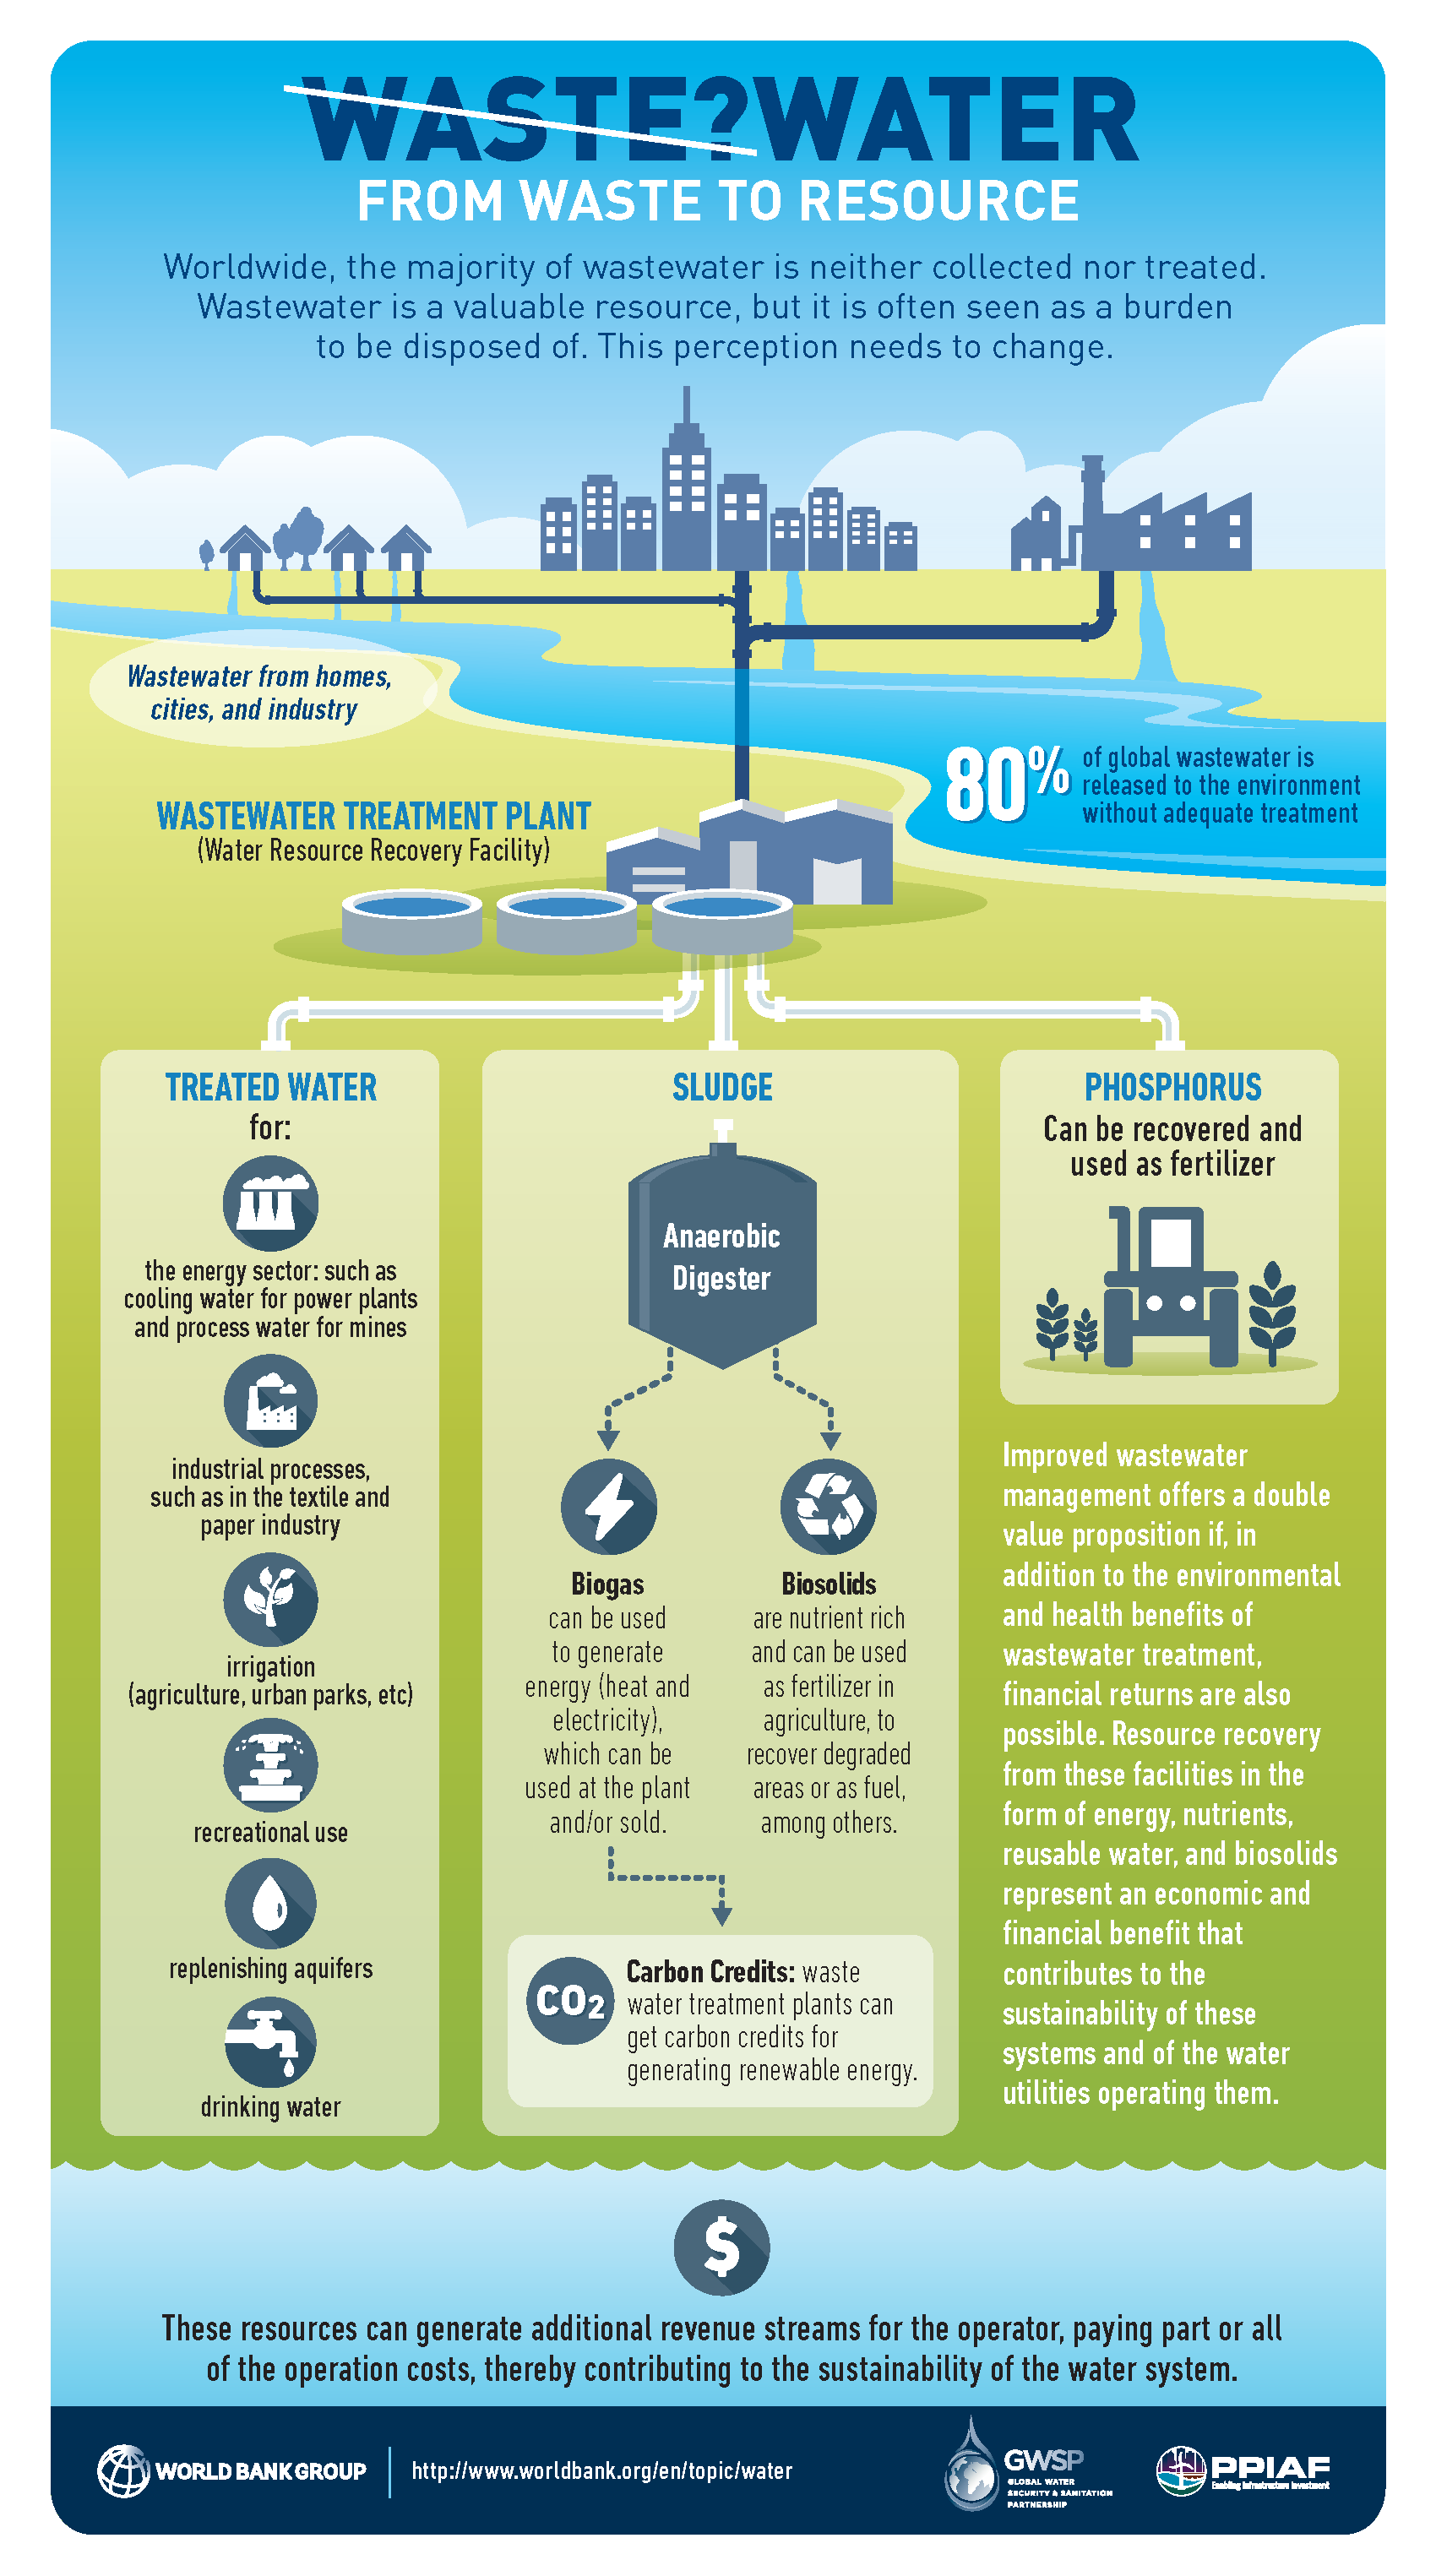
\includegraphics[scale=0.55]{WBWasteWaterResourceinfographic.png}\\
\emph{Source:  Waste to Resource - World Bank}\\
\end{center}









%\chapterimage{CareerChapterImage2.png}
\chapter{Wastewater Treatment - Careers}

\begin{itemize}
\item A career in wastewater treatment provides prospects of a stable and well paid employment with added perk of protecting the environment and the health of the community.
\item Wastewater treatment plants are facing challenges to fill the positions created by the retirement of the baby boomers.  It is estimated 30-50\% of the current employees will retire within the next 10 years.
\item There are a variety of career paths which require different skill sets and training. From high school graduates to PhDs.
\item Although actual renumeration and benefits depend on the size and location of the plant, in general wastewater jobs offer above average wages
\end{itemize}
\vspace{0.3cm}
\begin{tabular}{ |p{5cm}|p{5cm}|p{5cm}|  }
 \hline
 \multicolumn{3}{|c|}{Partial List of Wastewater Career Positions} \\
 \hline
 \hline
Plant Operators   & Collections Workers    &Electrical Maintenance Worker\\
Mechanical Mntnc. Worker   & Construction Inspectors   &Laboratory Technician\\
Environmental Specialists  & Civil Engineers & Mechanical Engineers\\
Electrical Engineers  & Office Assistants & Public Info. Specialists\\
Instrumentation Mntnc. Worker   & Finance and Accounting &Contracts Administrators\\
Warehouse Workers & Buyer & Health and Safety Specialist\\
Surveyors & CAD and Graphics Designers & Planners and Schedulers\\
 \hline
\end{tabular}\\




%%\documentclass{article}
%%\usepackage[english]{babel}%
%\usepackage{graphicx}
%\usepackage{tabulary}
%\usepackage{tabularx}
%\usepackage[table,xcdraw]{xcolor}
%\usepackage{pdflscape}
%\usepackage{lastpage}
%\usepackage{multirow}
%\usepackage{afterpage}
%\usepackage{rotating}
%\usepackage{pdfpages}
%\usepackage{cancel}
%\usepackage{amsmath}
%\usepackage[table]{xcolor}
%\usepackage{caption}
%\captionsetup{font=scriptsize,labelfont=scriptsize}
%\usepackage{pdflscape}
%\usepackage{fixltx2e}
%\usepackage[T1]{fontenc}
%\usepackage[utf8]{inputenc}
%\usepackage{multirow}
%\usepackage{ifthen}
%\usepackage{fancyhdr}
%\usepackage[document]{ragged2e}
%\usepackage[margin=1in,top=1.2in,headheight=57pt,headsep=0.1in]
%{geometry}
%\usepackage{ifthen}
%\usepackage{fancyhdr}
%\everymath{\displaystyle}
%\usepackage[document]{ragged2e}
%\usepackage{fancyhdr}
%\usepackage[table,xcdraw]{xcolor}
%% If you use beamer only pass "xcolor=table" option, i.e. \documentclass[xcolor=table]{beamer}
%\usepackage[normalem]{ulem}
%\useunder{\uline}{\ul}{}
%\everymath{\displaystyle}
%\linespread{2}%controls the spacing between lines. Bigger fractions means crowded lines%
%%\pagestyle{fancy}
%%\usepackage[margin=1 in, top=1in, includefoot]{geometry}
%%\everymath{\displaystyle}
%\linespread{1.3}%controls the spacing between lines. Bigger fractions means crowded lines%
%%\pagestyle{fancy}
%\pagestyle{fancy}
%\setlength{\headheight}{56.2pt}
%
%
%\chead{\ifthenelse{\value{page}=1}{
\includegraphics[scale=0.3]{BassettCTCLogo}\\ \textbf \textbf Water - General Introduction}}
%\rhead{\ifthenelse{\value{page}=1}{Shabbir Basrai}{Shabbir Basrai}}
%\lhead{\ifthenelse{\value{page}=1}{}{\textbf Water - General Introduction}}
%
%
%\cfoot{}
%\lfoot{Page \thepage\ of \pageref{LastPage}}
%\rfoot{}
%\renewcommand{\headrulewidth}{2pt}
%\renewcommand{\footrulewidth}{1pt}
%\newcommand{\comment}[1]{\hspace{0em}{\small\textit{#1}}\bigskip\par}
%\begin{document}


\chapterimage{MathCover.png}
\chapter{Glossary}

ACID :  (1)    A substance that tends to lose a proton. (2)     A substance that dissolves in water with the formation of hydrogen ions. (3)    A substance containing hydrogen which may be replaced with metals to form salts. (4)   A substance that is corrosive.  (5)   A substance that may lower pH\\
\vspace{0.15cm}
ACIDITY :  (A) Measure of the ability to neutralize alkaline (hi pH) substances. (B)  The capacity of water or wastewater to neutralize bases. Acidity is expressed in milligrams per liter of equivalent calcium carbonate.\\
\vspace{0.15cm}
ACRE FOOT :  A volume of water one (1) foot deep and one (1) acre in area, or 43,560 cubic feet.\\
\vspace{0.15cm}
ACTIVATED CARBON :  Form of carbon processed to have small, low–volume pores that increase the surface area available for adsorption or chemical reactions.\\
\vspace{0.15cm}
ACTIVATED SLUDGE :   (A) A biological water treatment technology commonly used in municipal wastewater treatment systems. Sometimes private industry will harness this technique to reduce certain pollutants, such as BOD and COD (see definitions below), but usually only due to compliance concerns.  (B) Sludge withdrawn from the secondary clarifier in the activated sludge process, consisting of micro–organisms, non–living organic matter, and inorganic materials.\\
\vspace{0.15cm}
ACTIVATED SLUDGE PROCESS :   A common method of disposing of pollutants in biological wastewaters. In the process, large quantities of air are bubbled through wastewaters that contain dissolved organic substances in open aeration tanks. Bacteria and other types of microorganisms present in the system need oxygen to live, grown, and multiply in order to consume the dissolved organic "food" or pollutants in the waste. After several hours in a large holding tank, the water is separated from the sludge of bacteria and discharged from the system. Most of the activated sludge is returned to the treatment process, while the remainder is disposed of by one of several acceptable methods.\\
\vspace{0.15cm}
ACTUATOR :   Device used to operate a valve using electric, pneumatic or hydraulic means. Often used for remote control or sequencing of valve operations.\\
\vspace{0.15cm}
ADAPTER SPOOL :   An extension which is added to a short face–to–face valve, to conform to standard API 6D face–to–face dimensions.\\
\vspace{0.15cm}
ADVANCED WASTE TREATMENT :  (A) A treatment technology used to produce an extremely high–quality discharge.  (B) Any process of water renovation that upgrades treated wastewater to meet specific reuse requirements. Typical processes include chemical treatment and pressure filtration.  Also called tertiary treatment.\\
\vspace{0.15cm}
AERATION :   (A) The process of bringing about intimate contact between air and a liquid. (B) The process of adding air to wastewater to provide dissolved oxygen for aerobic bacterial treatment, to freshen wastewater and to keep solids in suspension.\\
\vspace{0.15cm}
AERATION TANK :   A chamber for injecting air into water.\\
\vspace{0.15cm}
AEROBES :  Bacteria that must have molecular (dissolved) oxygen (DO) to survive.\\
\vspace{0.15cm}
AEROBIC :  (A) A condition in which atmospheric or dissolved molecular oxygen is present in the aquatic (water) environment.  (B)  requiring free oxygen for respiration. Refers to types of bacteria commonly found in water and wastewater treatment systems.\\
\vspace{0.15cm}
AEROBIC BACTERIA :  Bacteria which will live and reproduce only in an environment containing oxygen which is available for their respiration (breathing), namely atmospheric oxygen or oxygen dissolved in water. Oxygen combined chemically, such as water molecules (H2O), cannot be used for respiration by aerobic bacteria.\\
\vspace{0.15cm}
AIR END :   A term referring to the side (or parts) of the pump that come into contact with shop/compressed air or natural gas. This applies to any air operated pump including Air Operated Diaphragm Pumps, air operated piston pumps and air operated drum pumps.\\
\vspace{0.15cm}
AIR LIFT :  A type of pump. This device consists of a vertical riser pipe in the wastewater or sludge to be pumped. Compressed air is injected into a tall piece at the bottom of the pipe.   Fine air bubbles mix with the wastewater or sludge to form a mixture lighter than the surrounding water which causes the mixture to rise in the discharge pipe to the outlet. An air–lift pump works like the center of a stand in a percolator coffee pot.\\
\vspace{0.15cm}
AIR TEST :  A method of inspecting a sewer pipe for leaks. Inflatable or similar plugs are placed in the line, and the space between these plugs is pressurized with air. A drop in pressure indicates the line or run being tested has leaks. \\
\vspace{0.15cm}
AIR: operated ejectors or centrifugal pumps. \\
\vspace{0.15cm}
ALGAE :  A class of microscopic plant life that contain chlorophyll, live floating (suspended) in water or are attached to rocks, walls and other surfaces, and grow and multiply through photosynthesis. Algae produce oxygen during sunlight hours, use oxygen during darkness and affect the pH and DO levels in water.\\
\vspace{0.15cm}
ALGAL BLOOM :  Sudden, massive growths of algae that develop in lagoons, lakes and reservoirs.\\
\vspace{0.15cm}
ALIQUOT :  Portion of a sample. Often an equally divided portion of a sample.\\
\vspace{0.15cm}
ALKALINITY :   The capacity of water to neutralize acids, a property imparted by the water’s content of carbonates, bicarbonates, hydroxides, and occasionally borates, silicates, and phosphates. Alkaline fluids have a pH value over 7.\\
\vspace{0.15cm}
ALL WELDED CONSTRUCTION :   Pertains to a valve construction in which the body is completely welded and cannot be disassembled and repaired in the field.\\
\vspace{0.15cm}
ANAEROBIC :   A biological environment that is deficient in all forms of oxygen, especially molecular oxygen, nitrates and nitrites. The decomposition by microorganisms of waste organic matter in wastewater in the absence of dissolved oxygen is classed as anaerobic.\\
\vspace{0.15cm}
ANAEROBIC BACTERIA :  Bacteria that live and reproduce in an environment containing no “free” or dissolved oxygen. Anaerobic bacteria obtain their oxygen supply by breaking down chemical compounds which contain oxygen, such as sulfate (SO 2–).\\
\vspace{0.15cm}
ANAEROBIC DECOMPOSITION :  The decay or breaking down of organic material in an environment containing no “free” or dissolved oxygen. \\
\vspace{0.15cm}
ANAEROBIC DIGESTION :  Anaerobic bacteria (saprophytic and methane fermenters) decompose wastewater solids (complex organic material) in two steps into – 1) volatile acids, and 2) methane gas, carbon dioxide and water in the absence of dissolved oxygen. Specially designed basins, digesters, are used to carry out the digestion processes, prevent air from entering and to capture the methane gas. The sludge layer at the bottom of lagoons provides for similar solids stabilization processes.\\
\vspace{0.15cm}
ANCHOR PIN :   A pin welded onto the body of ball valves. This pin aligns the adapter plate and restrains the plate and gear operator from moving while the valve is being operated.\\
\vspace{0.15cm}
ANGLE VALVE :   A variation of the globe valve, in which the end connections are at right angles to each other, rather than being inline.\\
\vspace{0.15cm}
ANIONIC FLOCCULANT :  Negatively charged flocculant. Used in water treatment to aid solid / liquid separation\\
\vspace{0.15cm}
ANOXIC :   A biological environment that is deficient in molecular oxygen, but may contain chemically bound oxygen, such as nitrates and nitrites.\\
\vspace{0.15cm}
ANOXIC :  Description of an environment without oxygen. In wastewater treatment anoxic processes are typically used for the removal of nitrogen from wastewater.\\
\vspace{0.15cm}
ANTISCALENT :  Material used to control scale formation in water systems such as boiler or cooling water systems.\\
\vspace{0.15cm}
AOD :   AOD stands for Air Operated Diaphragm (pump). These types of pumps are powered by compressed air or gas, making them ideal for hazardous applications such as petroleum based products and other flammable materials. With certain materials of construction, such as steel or conductive plastics, they are easily converted into fully explosion proof (Ex–Proof) pumps. Additionally, they can pull a suction lift and are submersible when installed properly. AOD’s can also handle slurries with solids concentrations up to 30% and can be run against a closed suction or “dead head” situation.\\
\vspace{0.15cm}
AODD :   AODD stands for Air Operated Double Diaphragm (pump). These types of pumps are powered by compressed air or gas, making them ideal for hazardous applications such as petroleum based products and other flammable materials. With certain materials of construction, such as steel or conductive plastics, they are easily converted into fully explosion proof (Ex–Proof) pumps. Additionally, they can pull a suction lift and are submersible when installed properly. AOD’s can also handle slurries with solids concentrations up to 30% and can be run against a closed suction or “dead head” situation.\\
\vspace{0.15cm}
AQUIFER :  A natural underground layer of porous materials usually capable of yielding a supply of water.\\
\vspace{0.15cm}
ARSENIC :   A heavy metal commonly regulated by wastewater discharge permits, but not commonly found in industrial wastewaters. Other heavy metals include – Cadmium (Cd), Chromium(Cr), Copper (Cu), Lead (Pb), Nickel (Ni), and Zinc (Zn).\\
\vspace{0.15cm}
ASPHYXIATION :  An extreme condition often resulting in death due to a lack of oxygen and excess carbon dioxide in the blood from any cause. \\
\vspace{0.15cm}
AVAILABLE CHLORINE :  The amount of chlorine available in compound chlorine sources compared with that of elemental (liquid or gaseous) chlorine.\\
\vspace{0.15cm}
AVERAGE MONTHLY DISCHARGE LIMITATION :  The highest allowable discharge over a calendar month \\
\vspace{0.15cm}
AVERAGE WEEKLY DISCHARGE LIMITATION :  The highest allowable discharge over a calendar week. \\
\vspace{0.15cm}
B.R.V. :  BODY RELIEF VALVE –  A relief valve (optional) installed on ball valves used in liquid service to provide for the relief of excess body pressure caused by thermal expansion.\\
\vspace{0.15cm}
BACK WASH :  Part of water filter, ion exchange or softener cycle that lifts up media bed to release and wash away dirt and other foulants.\\
\vspace{0.15cm}
BACKFILL :  (1) Material used to full in a trench or excavation. (2) The act of filling a trench or excavation, usually after a pipe or some type of structure has been placed in the trench or excavation. \\
\vspace{0.15cm}
BACKFILL COMPACTION :  (1) Tamping, rolling or otherwise mechanically compressing material used as backfill for a trench of excavation. Backfill is compressed to increase its density so that it will support the weight of machinery or other loads after the material is in place  excavation. (2) Compaction of a backfill material can be expressed as a percentage of the maximum compatibility, density or load capacity of the material being used. \\
\vspace{0.15cm}
BACKFLOW :  A reverse flow condition, created by a difference in water pressures, which causes water to flow back into the distribution pipes of a potable water supply from any source or sources other than an intended source. Also see BACKSIPHONAGE.\\
\vspace{0.15cm}
BACKFLUSHING :  A procedure used to wash settled waste matter off upstream to prevent odors from developing after a main line stoppage has been cleared. \\
\vspace{0.15cm}
BACKSEAT :   A Shoulder on the stem of a valve which seals against a mating surface inside the bonnet to permit replacement, under pressure, of stem seals or packing.\\
\vspace{0.15cm}
BACKSIPHONAGE :  A form of backflow caused by a negative or below atmospheric pressure within a water system. Also see BACKFLOW.\\
\vspace{0.15cm}
BACTERIA :   Bacteria are microscopic living organisms They are a group of universally distributed, rigid, essentially unicellular, microscopic organisms lacking chlorophyll. They are characterized as spheroids, rod–like, or curved entities, but occasionally appearing as sheets, chains, or branched filaments.\\
\vspace{0.15cm}
BAFFLE :  A flat board or plate, deflector, guide or similar device constructed or placed in flowing water, wastewater, or slurry systems to cause more uniform flow velocities, to absorb energy, and to divert, guide, or agitate liquids (water, chemical solutions, slurry).\\
\vspace{0.15cm}
BALL :   The spherical closure element of a ball valve.\\
\vspace{0.15cm}
BALL CHECK :   A fitting with a small ball that seals against a seat preventing flow in one direction and allowing flow in the other direction.\\
\vspace{0.15cm}
BALL VALVE :   A valve using a spherical closure element (ball) which is rotated thru 90° to open and close the valve.\\
\vspace{0.15cm}
BALLING :  A method of hydraulically cleaning a sewer or storm drain by using the pressure of a water head to create a high cleansing velocity of water around the ball. In normal operation, the ball is restrained by a cable while water washes past the ball at high velocity. Special sewer cleaning balls have an outside tread that causes them to spin or rotate, resulting in a “scrubbing” action of the flowing water along the pipe wall. \\
\vspace{0.15cm}
BAR RACK :  A screen composed of parallel bars, either vertical or inclined, placed in a sewer or other waterway to catch debris. The screenings may be raked from it. \\
\vspace{0.15cm}
BARREL :  (1) The cylindrical part of a pipe that may have a bell on one end. (2) The cylindrical part of a manhole between the cone at the top and the shelf at the bottom. \\
\vspace{0.15cm}
BASE :  (1)    A substance which takes up or accepts protons.  (2)    A substance which dissociates (separates) in aqueous solution to yield hydroxyl ions (OH–).  (3)    A substance containing hydroxyl ions which reacts with an acid to form a salt or which may react with metalsvto form precipitates.  (4)    A substance that may raise pH.\\
\vspace{0.15cm}
BASE :  A substance that takes up or accepts protons, dissociates in water to produce hydroxyl (OH–) ions, reacts with metals and is corrosive.\\
\vspace{0.15cm}
BDV :  BLOW DOWN VALVE –  A small ball valve that is installed on the aboveground end of an extended drain line. This valve also serves to vent body cavity pressure in the "block and bleed" mode.\\
\vspace{0.15cm}
BEDDING :  The prepared base or bottom of a trench or excavation on which a pipe or other underground structure is supported. \\
\vspace{0.15cm}
BEDDING COMPACTION :  (1) Tamping, rolling or otherwise mechanically compressing material used as bedding for a pipe or other underground structure to a density that will support expected loads. (2) Bedding compaction can be expressed as a percentage of the maximum load capacity of the bedding material. (3) Bedding compaction also can be expressed in load capacity or pounds per square foot. \\
\vspace{0.15cm}
BEDDING GRADE :  (1) In a gravity–flow sewer system, pipe bedding is constructed and compacted to the design grade of the pipe. This is usually expressed in a percentage. A 0.5 percent grade would be a drop of one–half of foot per hundred feet of pipe. (2) Bedding grade for a gravity–flow sewer pipe can also be specified as elevation above mean sea level at specific points. \\
\vspace{0.15cm}
BELL :  (1) In pipe fitting, the enlarged female end of a pipe into which the male end fits. (2) In plumbing, the expanded female end of a wiped joint. \\
\vspace{0.15cm}
BELL: AND–SPIGOT JOINT – A form of joint used on pipes which have an enlarged diameter or bell at one end, and a spigot at the other which fits into and is laid in the bell. The joint is then made tight by lead, cement, rubber O–ring, or other jointing compounds or materials. \\
\vspace{0.15cm}
BELLEVILLE SPRING :   A spring resembling a dished washer, used in some ball valves to push the seats against the ball.\\
\vspace{0.15cm}
BERM :  The earthen dike that surrounds ponds, lagoons and containment areas for hazardous material.\\
\vspace{0.15cm}
BEST EFFICIENCY POINT (B.E.P.) :   The point on a pump’s performance curve that corresponds to the highest efficiency.  \\
\vspace{0.15cm}
BEVEL GEAR OPERATOR :   Device facilitating operation of a gate or globe valve by means of a set of bevel gears having the axis of the pinion gear at right angles to that of the larger ring gear. The reduction ratio of this gearsetdetermines the multiplication of torque achieved.\\
\vspace{0.15cm}
BHP :   BHP is the actual amount of horsepower being consumed by the pump as measured on a pony brake or dynamometer.\\
\vspace{0.15cm}
BIOCHEMICAL OXYGEN DEMAND (BOD) :   A quantitative measure of the oxygen needed by bacteria and micro–organisms for the biological oxidation of organic wastes in a unit volume of wastewater. BOD is generally measured in milligrams per liter (mg/l) of oxygen consumed over a five day period. Although complete biological decomposition of organic waste requires about 20 days, the five day BOD is about two–thirds of the total oxygen required and, therefore, is a practical measure of waste concentration. In waste treatment language, BOD is most frequently stated as the percentage removed during treatment, or remaining after treatment.\\
\vspace{0.15cm}
BIOCIDE :  Chemical substance designed for killing living organisms in water. Often characterized by type of organism killed – bactericide, fungicide or algaecide.\\
\vspace{0.15cm}
BIOLOGICAL OXIDATION :   The process by which bacteria and other types of microorganisms consume dissolved oxygen and organic substances in biological wasterwater.  The energy released is then used to convert organic carbon into carbon dioxide and cellular material. \\
\vspace{0.15cm}
BIOMASS :  Amass or clump of living organisms feeding on wastes in wastewater, dead organisms and other debris. The mass may protect the organisms, as well as store food supplies. Also called ZOOGLEAL MASS.\\
\vspace{0.15cm}
BIOSOLIDS :  A primarily organic solid product, produced by wastewater treatment processes, that can be beneficially recycled. The word biosolids is replacing the word sludge.\\
\vspace{0.15cm}
BIOSOLIDS CAKE :  Solid discharge from a dewatering apparatus. \\
\vspace{0.15cm}
BIT :  (1) Cutting blade used in rodding (pipe cleaning) operations. (2) Cutting teeth on the auger head of a sewer boring tool. \\
\vspace{0.15cm}
BLANK :  A bottle containing only dilution water or distilled water, but the sample being tested is not added. Tests are frequently run on a SAMPLE and a BLANK and the differences are compared.\\
\vspace{0.15cm}
BLOCK AND BLEED :   The capability of obtaining a seal across the upstream and downstream seat rings of a valve when the body pressure is bled off to atmosphere thru blow down valves or vent plugs. Useful in testingfor integrityof seat seals and in accomplishing minor repairs under pressure.\\
\vspace{0.15cm}
BLOCKAGE :  (1) Partial or complete interruption of flow as a result of some obstruction in a sewer. (2) When a collection system becomes plugged and the flow backs up, “blockage.” \\
\vspace{0.15cm}
BLOW DOWN (BLEED: off) – terms to describe the deliberate rejection of water from a system such as boiler or cooling water system. Typically done to control system’s water total dissolved system or conductivity.\\
\vspace{0.15cm}
BLUE: GREEN ALGAE – Varieties of algae characterized by their bluish–green color. The appearance of blue–green algae indicates unhealthy conditions in lagoon cells, often associated with organic overloading and lack of adequate dissolved oxygen.\\
\vspace{0.15cm}
BOD :  Biochemical Oxygen Demand. The rate at which organisms use the oxygen in water or wastewater while stabilizing decomposable organic matter under aerobic conditions. In decomposition, organic matter serves as food for the bacteria and energy results from its oxidation. BOD measurements are used as a measure of the organic strength of wastes in water. \\
\vspace{0.15cm}
BODY :   The principal pressure containing part of a valve, in which the closure element and seats are located.\\
\vspace{0.15cm}
BOLTED BONNET :   A bonnet which is connected to a valve body with bolts or studs and nuts.\\
\vspace{0.15cm}
BOLTED CONSTRUCTION :   Describes a valve construction in which the pressure shell elements are bolted together, and thus can be taken apart and repaired in the field.\\
\vspace{0.15cm}
BONNET :   The top part of a valve, attached to the body, which contains the packing gland, guides the stem, and adapts to extensions or operators.\\
\vspace{0.15cm}
BORE (OR PORT) :   The inside diameter of the smallest opening through a valve, e.g., inside diameter of a seat ring, diameter of hole through ball in a ball valve.\\
\vspace{0.15cm}
BRANCH MANHOLE :  A sewer or drain manhole which has more than one pipe feeding into it. A standard manhole will have one outlet and one inlet. A branch manhole will have one outlet and two or more inlets. \\
\vspace{0.15cm}
BRANCH SEWER :  A sewer that receives wastewater from a relatively small area and discharges into a main sewer servicing more than one branch sewer area. \\
\vspace{0.15cm}
BUBBLE: TIGHT SHUT–OFF –  A phrase used in describing the sealing ability of a valve. During air pressure testing of a new valve in the closed position, leakage past the seats is collected and bubbled thru water. To qualify as "bubble tight," no bubbles should be observed in a prescribed time span.\\
\vspace{0.15cm}
BUCKET :  (1) A special device designed to be pulled along a sewer for the removal of debris from the sewer. The bucket has one end open with the opposite end having a set of jaws. When pulled from the jaw end, the jaws are automatically opened. When pulled from the other end, the jaws close. In operation, the bucket is pulled into the debris from the jaw end and to a point where some of the debris has been forced into the bucket. The bucket is then pulled out of the sewer from the other end, causing the jaws to close and retain the debris. Once removed from the manhole, the bucket is emptied and the process repeated. (2) A conventional pail or bucket used in BUCKETING OUT and also for lowering and raising tools and materials from manholes and excavations. \\
\vspace{0.15cm}
BUCKET BAIL :  The pulling handle on a bucket machine. \\
\vspace{0.15cm}
BUCKET MACHINE : A powered winch machine designed for operation over a manhole. The machine controls the travel of buckets used to clean sewers. \\
\vspace{0.15cm}
BUCKETING OUT :  An expression used to describe removal of debris from a manhole with a pail on a rope. In balling or high–velocity cleaning of sewers, debris is washed into the downstream manhole. Removal of this debris by scooping it into pails and hauling debris out is called “bucketing out.” \\
\vspace{0.15cm}
BUFFER :  A solution or liquid whose chemical makeup neutralizes acids or bases without a great change in pH.\\
\vspace{0.15cm}
BULKING :  Clouds of billowing sludge that occur throughout secondary clarifiers and sludge thickeners when the sludge does not settle properly.   In the activated sludge process bulking is usually caused by filamentous bacteria or bound water.\\
\vspace{0.15cm}
BULKING SLUDGE :   A phenomenon that occurs in activated sludge plants whereby the sludge occupies excessive volumes and will not concentrate readily. This condition refers to a decrease in the ability of the sludge to settle and consequent loss over the settling tank weir. Bulking in activated sludge aeration tanks is caused mainly by excess suspended solids (SS) content. Sludge bulking in the final settling tank of an activated sludge plant may be caused by improper balance of the BOD load, SS concentration in the mixed liquor, or the amount of air used in aeration.\\
\vspace{0.15cm}
BURIED SERVICE :   An application in which valves are installed in lines which are buried below ground level.\\
\vspace{0.15cm}
BUTT WELD END (BWE) :   The end connection of a valve suitably prepared for butt welding to a connecting pipe.\\
\vspace{0.15cm}
BUTTERFLY VALVE :   A short face–to–face valve which has a movable vane, in the center of the flow stream, which rotates 90 degrees as the butterfly valve opens and closes.\\
\vspace{0.15cm}
BVR :  BALL VALVE REGULATOR –  An automatic throttling valve controlling flow or pressure in a pipeline; comprising a package involving al ball valve actuator, positioner, and controlling instrument.\\
\vspace{0.15cm}
BYPASS :   A system of pipes and valves permitting the diversion of flow or pressure around a line valve.\\
\vspace{0.15cm}
BYPASS :  A pipe, valve, gate, weir, trench or other device designed to permit all or part of a wastewater flow to be diverted from usual channels or flow. Sometimes refers to a special line which carries the flow around a facility or device that needs maintenance or repair. \\
\vspace{0.15cm}
BYPASSING :  The act of causing all or part of a flow to be diverted from its usual channels. In a wastewater treatment plant, overload flows should be bypassed into a holding pond for future treatment. 224 \\
\vspace{0.15cm}
CADMIUM :   A heavy metal commonly regulated by wastewater discharge permits and typically found in the metal finishing industry.  Other heavy metals include – Arsenic (As), Chromium(Cr), Copper (Cu), Lead (Pb), Nickel (Ni), and Zinc (Zn).\\
\vspace{0.15cm}
CAKE SOLID DISCHARGE RATE :  The dry solids cake discharge from a centrifuge, which is expressed as: dry cake solids discharge rate = (dry solids feed rate) x (solids recovery). \\
\vspace{0.15cm}
CALCIUM AND MAGNESIUM SOAPS, MINERAL OILS, AND CERTAIN OTHER NON: fatty material which tend to separate from water and coagulate as floatables or scums. \\
\vspace{0.15cm}
CARBON DIOXIDE :  A common gas, CO2, found abundantly in air, is a product of bacterial respiration and used by algae in photosynthesis. The concentration of carbon dioxide in the lagoon water governs the pH of the lagoon.\\
\vspace{0.15cm}
CARCINOGEN :  Any substance that tends to produce cancer in an organism.\\
\vspace{0.15cm}
CASING :   The body of the pump which encloses the impeller. Primarily used in reference to centrifugal pumps.\\
\vspace{0.15cm}
CAST :   The form of a particular part of a valve, where the basic shape is formed by molding rather than fabricating.\\
\vspace{0.15cm}
CASTING :   A product or the act of producing a product made by pouring molten metal into a mold and allowing it to solidify, thus taking the shape of the mold.\\
\vspace{0.15cm}
CATCH BASIN :  A chamber or well used with storm or combined sewers as a means of removing grit which might otherwise enter and be deposited in sewers. \\
\vspace{0.15cm}
CATIONIC FLOCCULANT :  Positively charged high molecular weight polyelectrolyte water soluble organic polymer designed to agglomerate solids in water substrates.\\
\vspace{0.15cm}
CAVITATION :  The formation and collapse of a gas pocket or bubble on the blade of an impeller or gate of a valve. The collapse of the bubble drives water into the impeller or gate with a terrific force that can cause pitting of the surface. Cavitation is indicated by loud hammering noises.\\
\vspace{0.15cm}
CENTRIFUGAL FORCE :   A force associated with a rotating body. In the case of a pump, the rotating impeller pushes fluid on the back of the impeller blade, imparting motion. Since the motion is circular there is a centrifugal force associated with it. The force pushes the fluid against a fixed pump casing thereby pressurizing the fluid and forcing it through the outlet.\\
\vspace{0.15cm}
CENTRIFUGAL PUMP :   Centrifugal pumps are the most common type of pump in use today throughout the world. A centrifugal pump is a rotodynamic pump that uses a rotating impeller to increase the velocity of a fluid. Centrifugal pumps are commonly used to move liquids through a piping system. The fluid enters the pump impeller along or near to the rotating axis and is accelerated by the impeller, flowing radially outward into a diffuser or volute chamber, from there it exits into the downstream piping system. A centrifugal pump works by the conversion of the rotational kinetic energy, typically from an electric motor or engine, to an increased static fluid pressure. This action is described by Bernoulli’s principle. The rotation of the pump impeller imparts kinetic energy to the fluid as it is drawn in from the impeller eye (center) and is forced outward through the impeller vanes to the periphery. As the fluid exits the impeller, the fluid kinetic energy (velocity) is then converted to (static) pressure due to the change in area the fluid experiences in the volute section. Typically, the volute shape of the pump casing (increasing in volume), or the diffuser vanes (which serve to slow the fluid, converting to kinetic energy in to flow) are responsible for the energy conversion. The energy conversion results in an increased pressure on the downstream side of the pump, causing flow.\\
\vspace{0.15cm}
CENTRIFUGE :  A mechanical device that uses centrifugal or rotational forces to separate solids from liquids.\\
\vspace{0.15cm}
CHAIN WHEEL OPERATED VALVE :   An overhead valve operated by a chain drive wheel instead of a handwheel.\\
\vspace{0.15cm}
CHARACTERIZED GATE OR BALL :   A ball or gate, the shape of whose port has been specially altered to provide a specific throttling capability.\\
\vspace{0.15cm}
CHECK VALVE :   A one–directional valve which is opened by the fluid flow in one direction and closed automatically when the flow stops or is reversed.\\
\vspace{0.15cm}
CHEMICAL GROUT :  Two chemical solutions that form a solid when combined. Solidification time is controlled by the strength of the mixtures used and the temperature. \\
\vspace{0.15cm}
CHEMICAL OXYGEN DEMAND (COD) :   A quantitative measure of the amount of oxygen required to oxidize all organic compounds in a unit volume on wastewater – non–biodegradable as well as the BOD. The COD level can be determined more readily than BOD, but this measurement does not indicate how much of the waste can be decomposed by biological oxidation.\\
\vspace{0.15cm}
CHLORINATION :   The application of chlorine to water, sewage, or industrial wastes, generally for the purpose of disinfection, but frequently for accomplishing other chemical or biological wasterwater treatment results.\\
\vspace{0.15cm}
CHLORINATOR :  A metering device which is used to add chlorine to water.\\
\vspace{0.15cm}
CHLORINE CONTACT UNIT :  A baffled basin that provides sufficient time for disinfection to occur.\\
\vspace{0.15cm}
CHLORINE DEMAND :  Chlorine demand is the difference between the amount of chorine added to wastewater and the amount of residual chlorine remaining after a given contact time. Chlorine demand may change with dosage, time temperature, pH, and nature and amount of the impurities in the water.\\
\vspace{0.15cm}
CHLORINE REQUIREMENT :    The amount of chlorine which is needed for a particular purpose. Some reasons for adding chlorine are reducing the number of coliform bacteria (Most Probable Number), obtaining a particular chlorine residual, or oxidizing some substance in the water. In each case a definite dosage of chlorine will be necessary. This dosage is the chlorine requirement.\\
\vspace{0.15cm}
CHLORINE RESIDUAL :  The amount of free chlorine remaining after meeting chlorine demand under given conditions and is necessary to complete disinfection.\\
\vspace{0.15cm}
CHOPPER PUMP :   A chopper pump is a centrifugal pump, which is equipped with a cutting system to facilitate chopping/maceration of solids that are present in the pumped liquid. The main advantage of this type of pump is that it prevents clogging of the pump itself and of the adjacent piping, as all the solids and stringy materials are macerated by the chopping system. Chopper pumps exist in various configurations, including submersible and dry–installed design and they are typically equipped with an electric motor to run the impeller and to provide torque for the chopping system. Due to its high solids handling capabilities, the chopper pump is often used for pumping sewage, sludge, manure slurries, and other liquids that contain large or tough solids.\\
\vspace{0.15cm}
CHROMIUM :   A heavy metal commonly regulated by wastewater discharge permits and found in metals–related industries and products (including stainless steel). It is typically regulated in two forms – total chromium and hexavalent chromium. Other heavy metals include – Arsenic (As), Cadmium (Cd), Copper (Cu), Lead (Pb), Nickel (Ni), and Zinc (Zn).\\
\vspace{0.15cm}
CITY GATE :  CITY GATE STATION –  The metering and pressure reducing station where gas is transferred from a high pressure cross–country transmission line to a low pressure distribution piping system within a city.\\
\vspace{0.15cm}
CLAPPER :   The hinged closure element of a swing check valve.\\
\vspace{0.15cm}
CLARIFICATION :  Any process or processes used to reduce the concentration of suspended matter in a liquid, such as quiescent settling or sedimentation. Lagoons provide clarification across the cells and in quiescent zones in aerated systems, allowing solids to settle into a sludge layer\\
\vspace{0.15cm}
CLARIFIER :   A large, circular or rectangular tank that separates solids from the waste stream by settling or flotation.\\
\vspace{0.15cm}
CLEAN IN PLACE (CIP) :  Method of cleaning the interior surfaces of pipes, vessels, process equipment, filters and associated fittings, without disassembly.\\
\vspace{0.15cm}
CLEAN WATER ACT :  Federal legislation passed in 1972 creating the Environmental Protection Agency, requiring a nationwide system for controlling pollutant discharges and providing for construction and regulation of publicly owned treatment works.\\
\vspace{0.15cm}
CLEANOUT :  An opening (usually covered or capped) in a wastewater collection system used for inserting tools, rods or snakes while cleaning a pipeline or clearing a stoppage. \\
\vspace{0.15cm}
CLOSURE ELEMENT :   The moving part of a valve, positioned in the flowstream which controls flow thru the valve. Ball. Gate, Plug, Clapper, Disc, etc., are specific names for closure elements.\\
\vspace{0.15cm}
CO: precipitation – Term to describe compound used in water treatment to aid precipitation of substances normally soluble under the conditions employed. Common co–precipitants used in water are iron, aluminum, calcium and magnesium.\\
\vspace{0.15cm}
COAGULANTS :  Chemicals that cause very fine particles to clump (floc) together into larger particles. This makes it easier to separate the solids from the water by settling, skimming, draining or filtering.\\
\vspace{0.15cm}
COAGULATION :   The agglomeration of colloidal or suspended matter brought about by the addition of some chemical to the liquid, by contact, or by other means.  Involves destabilization for repulsive electrical charges to permit agglomeration of colloid particles in water. This process aids the clarification of water.\\
\vspace{0.15cm}
COLIFORM :  A type of bacteria. The presence of coliform–group bacteria is an indication of possible pathogenic bacterial contamination. The human intestinal tract is one of the main habitats of coliform bacteria. They may also be found in the intestinal tracts of warm–blooded animals, and in plants, soil, air, and the aquatic environment. Fecal coliforms are those coliforms found in the feces of various warm–blooded animals; whereas the term “coliform” also includes various other environmental sources.\\
\vspace{0.15cm}
COLIFORM :  A type of bacteria. The presence of coliform–group bacteria is an indication of possible pathogenic bacterial contamination. The human intestinal tract is one of the main habitats of coliform bacteria. They may also be found in the intestinal tracts of warm–blooded animals, and in plants, soil, air, and the aquatic environment. Fecal coliforms are those coliforms found in the feces of various warm–blooded animals; whereas the term “coliform” also includes various other environmental sources.\\
\vspace{0.15cm}
COLIFORM BACTERIA :  Live in everyone’s intestinal track. They are considered non–pathogenic. \\
\vspace{0.15cm}
COLIFORM ORGANISMS :   A group of bacteria recognized as indicators of fecal pollution (see also escherichia coliform).\\
\vspace{0.15cm}
COLLECTION SYSTEM :  A network of pipes, manholes, cleanouts, traps, siphons, lift stations and other structures used to collect all wastewater and wastewater–carried wastes of an area and transport them to a treatment plant or disposal system. The collection system includes land, wastewater lines and appurtenances, pumping stations and general property. \\
\vspace{0.15cm}
COLORIMETRIC MEASUREMENT :  A means of measuring unknown chemical concentrations in water by MEASURING A SAMPLE’S COLOR INTENSITY. The specific color of the sample, developed by addition of chemical reagents, is measured with a photoelectric colorimeter or is compared with “color standards” using, or corresponding with, known concentrations of the chemical.\\
\vspace{0.15cm}
COLORIMETRIC MEASUREMENT :  A means of measuring unknown chemical concentrations in water by MEASURING A SAMPLE’S COLOR INTENSITY. The specific color of the sample, developed by addition of chemical reagents, is measured with a photoelectric colorimeter or is compared with “color standards” using, or corresponding with, known concentrations of the chemical.\\
\vspace{0.15cm}
COMBINED SEWER :   Carries both sanitary sewage and storm water run–off.\\
\vspace{0.15cm}
COMMINUTOR :  A device used to reduce the size of the solid chunks in wastewater by shredding (comminuting). The shredding action is like many scissors cutting or chopping to shreds all the large influent solids material in the wastewater.\\
\vspace{0.15cm}
COMMUNITY WASTEWATER SYSTEM :  A public wastewater system which has at least 15 service connection or treats 5,000 gallons or more of wastewater per day. The term “community wastewater system” is used only to identify the public wastewater systems which must be operated by certified operators. \\
\vspace{0.15cm}
COMPOSITE (PROPORTIONAL) SAMPLE :  A collection of individual samples obtained at regular intervals during a 24–hour period. Each individual sample is combined with the others in proportion to the rate of flow when the sample was collected. The resulting mixture, or composite, forms a representative sample and is analyzed to determine the average conditions during the sampling period.\\
\vspace{0.15cm}
COMPUTED PER CAPITA CONTRIBUTION : The computed wastewater contribution from a domestic area, based on the population of the area. In the United States, the daily average wastewater contribution is considered to be 100 gallons per capita per day (100GPCD). \\
\vspace{0.15cm}
COMPUTED TOTAL CONTRIBUTION :  The total anticipated load on a wastewater treatment plant or the total anticipated flow in any collection system area based on the combined computed contributions of all connections to the system. \\
\vspace{0.15cm}
CONCENTRATE :  The high TDS discharge from a reverse osmosis filtration process.\\
\vspace{0.15cm}
CONCRETE CRADLE :  A device made of concrete that is designed to support sewer pipe. 225 \\
\vspace{0.15cm}
CONDENSATE :  steam that has lost heat and condensed into water.\\
\vspace{0.15cm}
CONDUCTIVITY :  Transmittance of an electric current through water. Usually measured in microsiemens per centimeter (uS/cm) or micromho per centimeter (umho/cm).\\
\vspace{0.15cm}
CONFINED SPACE :  Confined space means a space that:  A.     Is large enough and so configured that an employee can bodily enter and perform assigned work; and B.    Has limited or restricted means for entry or exit; and C.     Is not designed for continuous employee occupancy.\\
\vspace{0.15cm}
CONTAMINATION :  The introduction into water of microorganisms, chemicals, toxic substances, wastes, or wastewater in a concentration that makes the water unfit for its next intended use.\\
\vspace{0.15cm}
CONTROL VALVE :   A valve that controls a process variable, such as pressure, flow or temperature by modulating its opening in response to a signal from a controller.\\
\vspace{0.15cm}
CONTROL VOLUME :   Limits imposed for the theoretical study of a system. The limits are usually set to intersect the system at locations where conditions are known.\\
\vspace{0.15cm}
CONTROLLER :   A device that measures a controlled variable, compares it with a predetermined setting and signals the actuator to read just the opening of the valve in order to re–establish the original control setting.\\
\vspace{0.15cm}
COPPER :   A heavy metal commonly regulated by wastewater discharge permits. It is found in the metal finishing and electrical industries. Other heavy metals include – Arsenic (As), Cadmium (Cd), Chromium(Cr), Lead (Pb), Nickel (Ni), and Zinc (Zn).\\
\vspace{0.15cm}
CORROSION :  The gradual decomposition or destruction of a material due to chemical action, often due to an electrochemical reaction. Corrosion starts at the surface of a material and moves inward, such as the chemical action upon manholes and sewer pipe materials. \\
\vspace{0.15cm}
CORROSION INHIBITOR :  chemical additive designed to control / minimize metal corrosion in water system.\\
\vspace{0.15cm}
COULISSE :   Of or using runners or slides as a guiding mechanism; as in a "Coulisse" style gate valve.\\
\vspace{0.15cm}
COUPLING :  (1) A threaded sleeve used to connect two pipes. (2) A device used to connect two adjacent parts, such as pipe coupling, hose coupling or drive coupling. \\
\vspace{0.15cm}
COUPON :  A steel specimen inserted into wastewater to measure the corrosiveness of the wastewater. The rate of corrosion is measured as the loss of weight of the coupon or change in its physical characteristics. Measure the weight loss (in milligrams) per surface area (in square decimeters) exposed to the wastewater per day. \\
\vspace{0.15cm}
CREST :  The bottom edge of a weir plate.\\
\vspace{0.15cm}
CROSS CONNECTION :  A connection between a drinking (potable) water system and an unapproved water supply. For example, if you have a pump moving nonpotable water and hook into the drinking water system to supply water for the pump seal, a cross connection or mixing between the two water systems can occur. This mixing may lead to contamination of the drinking water.\\
\vspace{0.15cm}
CROSS CONNECTION :  A connection between a drinking (potable) water system and an unapproved water supply. For example, if you have a pump moving nonpotable water and hook into the drinking water system to supply water for the pump seal, a cross connection or mixing between the two water systems can occur. This mixing may lead to contamination of the drinking water.\\
\vspace{0.15cm}
CROSS CONNECTION :  A connection between a storm drain system and a sanitary collection system. \\
\vspace{0.15cm}
CROSS: CONNECTION – A connection between a drinking water system and an unapproved system.\\
\vspace{0.15cm}
CRUSTACEANS :  A class of microscopic water animals that consume large quantities of bacteria and algae.\\
\vspace{0.15cm}
CRYOGENIC VALVE :   A valve capable of functioning at cryogenic temperatures.\\
\vspace{0.15cm}
CYANIDE :   A toxic element often found in wastewater from metal finishing industries. It’s commonly regulated by wastewater permits.\\
\vspace{0.15cm}
CYCLE :   A single complete operation or process returning to the starting point. A valve, stroked from full open to full close and back to full open, has undergone one cycle.\\
\vspace{0.15cm}
CYCLES OF CONCENTRATION :  Ratio of boiler or cooling water to make up (feed water). Typically measured by monitoring total dissolved solids, conductivity, silica or chlorides.\\
\vspace{0.15cm}
CYLINDER OPERATOR :   A power–piston valve operator using either hydraulic or pneumatic pressure. A sealed piston converts applied pressure into a linear piston rod (stem) motion.\\
\vspace{0.15cm}
DAILY DISHARGE :  The discharge of a pollutant measured during a calendar day or any 24 – hour period that reasonably represents a calendar day for the purposes of sampling. \\
\vspace{0.15cm}
DAILY MAXIUM DISCHARGE :  The highest allowable value for a daily discharge. \\
\vspace{0.15cm}
DAPHNIA :  A crustacean commonly found in wastewater lagoons.\\
\vspace{0.15cm}
DATUM PLANE :   A reference plane.   A conveniently accessible known surface from which all vertical measurements are taken or referred to.\\
\vspace{0.15cm}
DEADEND MANHOLE :  A manhole located at the upstream end of a sewer and having no inlet pipe. \\
\vspace{0.15cm}
DEBRIS :  Any material in wastewater found floating, suspended, settled, or moving along the bottom of a sewer. This material may cause stoppages by getting hung up on roots or settling out in a sewer. Debris includes grit, paper, rubber, silt, and all materials except liquid. \\
\vspace{0.15cm}
DECHLORINATION :  The removal of chlorine from the effluent of a treatment plant.\\
\vspace{0.15cm}
DECHLORINATION :  The removal of chlorine from the effluent of a treatment plant.\\
\vspace{0.15cm}
DECHLORINATION :  The removal of chlorine from the effluent of a treatment plant.\\
\vspace{0.15cm}
DEMULSIFIER (EMULSION BREAKER) :  Chemical additive that destroys the emulsifying characteristics water. Typically used separate stabilized (emulsified) oil in water.\\
\vspace{0.15cm}
DENITRIFICATION :   A biological process by which nitrate is converted to nitrogen gas.\\
\vspace{0.15cm}
DENITRIFICATION :  (1)     The anoxic biological reduction of nitrate nitrogen to nitrogen gas.  (2)     The removal of some nitrogen from a system.  (3)     An anoxic process that occurs when nitrite or nitrate ions are reduced to nitrogen gas and nitrogen bubbles are formed as a result of this process.\\
\vspace{0.15cm}
DENITRIFICATION :  (1)     The anoxic biological reduction of nitrate nitrogen to nitrogen gas.  (2)     The removal of some nitrogen from a system.  (3)   An anoxic process that occurs when nitrite or nitrate ions are reduced to nitrogen gas and nitrogen bubbles are formed as a result of this process.\\
\vspace{0.15cm}
DENITRIFICATION :  An anaerobic process that occurs when nitrite and nitrate ions are reduced to nitrogen gas and bubbles are formed. These bubbles attach to sludge flocs, causing rising sludge that floats to the surface of secondary clarifiers.\\
\vspace{0.15cm}
DENITRIFICATION :  Wastewater treatment process involved in the biological removal of nitrogen in which the nitrite (NO2) is converted to nitrogen gas (N2)\\
\vspace{0.15cm}
DEQ :  Department of Environmental Quality. \\
\vspace{0.15cm}
DETENTION TIME :  The theoretical time that water may stay in a basin such as lagoon. It is the total volume of the lagoon divided by the flow rate. Usually expressed in days of time or in hours.  The theoretical time water remains in a tank at a given discharge.  The time required to fill a tank at a given flow or the theoretical time required for a given flow of wastewater to pass through a tank.\\
\vspace{0.15cm}
DETRITUS :    The heavy, coarse mixture of grit and organic material carried by wastewater. (also called grit).\\
\vspace{0.15cm}
DEWATER :  To drain or remove water from an enclosure. A structure may be dewatered so that it can be inspected or repaired. Dewater also means draining or removing water from sludge to increase the solids concentration. 226 \\
\vspace{0.15cm}
DEWATERING :  Removing free water from a sludge or slurry to form a high solids cake. belt filter presses, centrifuges, rotary fan presses and vacuum presses are dewatering devices.\\
\vspace{0.15cm}
DEWATERING PUMP :   Any pump capable of removing water from an unwanted area. They are usually small, portable pumps that run on single phase power, compressed air or a small engine, but can be large permanently installed units as well.\\
\vspace{0.15cm}
DIAPHRAGM :   A round, thin flexible sealing device secured and sealed around its outer edge – and sometimes around a central hole in the diaphragm – with its unsupported area free to move by flexing.\\
\vspace{0.15cm}
DICHARGE MONITORING REPORT (DMR) :  The monthly report required by the treatment plant’s NPDES / OPDES discharge permit. \\
\vspace{0.15cm}
DIFFUSED: AIR AERATION – A diffused air activated sludge plant takes air, compresses it, and then discharges the air below the water surface of the aerator through some type of air diffusion device.\\
\vspace{0.15cm}
DIFFUSER :  A device used to break the air stream from the blower system into fine bubbles in an aeration tank or reactor.\\
\vspace{0.15cm}
DIGESTER :  A tank in which sludge is placed to allow decomposition by microorganisms. Digestion may occur under anaerobic (more common) or aerobic conditions.\\
\vspace{0.15cm}
DIGESTION :   The biochemical decomposition of organic matter that results in the formation of mineral and simpler organic compounds.\\
\vspace{0.15cm}
DIP :  A point in the sewer pipe where a drain grade defect results in a puddle of standing water when there is no flow. \\
\vspace{0.15cm}
DIP TUBE :   Extending the blow down valve on large gate valves requires a tube which is located inside of the valve. The tube is called the "dip tube" and extends through the bonnet to the bottom of the body cavity.\\
\vspace{0.15cm}
DISC :   The closure element of a globe angle or small regulator valve. The disc (sometimes referred to as "valve," "poppet" or "plug") moves to and from the seat in a direction perpendicular to the seat face. Depends on stem force for tight shutoff.\\
\vspace{0.15cm}
DISCHARGE STATIC HEAD :   The difference in elevation between the liquid level of the discharge tank and the centerline of the pump. This head also includes any additional head that may be present at the discharge tank fluid surface.\\
\vspace{0.15cm}
DISINFECTION :  The process designed to kill most microorganisms in water, including the destruction or inactivation of pathogenic bacteria. Disinfection differs from sterilization which destroys all living forms.\\
\vspace{0.15cm}
DISINFECTION :  The process designed to kill or inactivate most microorganisms in wastewater, including essentially all pathogenic (disease–casing) bacteria.   There are several ways to disinfect, with chlorination being the most frequently used in water and wastewater treatment plants.\\
\vspace{0.15cm}
DISINFECTION :  The process designed to kill or inactivate most microorganisms in wastewater, including essentially all pathogenic (disease–casing) bacteria.   There are several ways to disinfect, with chlorination being the most frequently used in water and wastewater treatment plants.\\
\vspace{0.15cm}
DISINFECTION :  The process designed to kill or inactivate most microorganisms in water, including essentially all pathogenic (disease–causing) bacteria. There are several ways to disinfect, with chlorine being the most frequently used method in both water and wastewater systems. \\
\vspace{0.15cm}
DISPERSANT :  A non–surface active compound or an active substance added to a suspension, usually a mix, to increase the separation of particles and to prevent subsiding or clumping.\\
\vspace{0.15cm}
DISSOLVED AIR FLOTATION :   A physical/chemical wastewater treatment technology that can be cost–effectively used by industry to remove FOG (fats, oils and grease), suspended solids, and some metals.\\
\vspace{0.15cm}
DISSOLVED AIR FLOTATION CLARIFIER (DAF) :  a piece of equipment that used dissolved air to float suspended solids from water. Typically used when the suspended solids have a lower density than water.\\
\vspace{0.15cm}
DISSOLVED OXYGEN (DO) :   The oxygen dissolved in water, wastewater, or other liquid. DO is measured in milligrams per liter. If the DO of a sample of water is 2 mg/L, it means that there are 2lbs of oxygen in 1 mil lb of water.\\
\vspace{0.15cm}
DISSOLVED SOLIDS :  The salts and other residues left after evaporation of water that has been passed through a laboratory filter. Dissolved solids cannot be filtered out. Some colloidal solids may not be in true solution, but if they pass through the standard membrane filter, they are considered dissolved solids. (See suspended solids)\\
\vspace{0.15cm}
DIURNAL :  Having a daily cycle; usually a 24–hour period from 12:00am to 12:00pm.\\
\vspace{0.15cm}
DO :  Dissolved Oxygen –  An indication of how much oxygen is present in water. If a facility discharges directly to a stream or river, it will usually have a permit limit related to dissolved oxygen.\\
\vspace{0.15cm}
DRAGLINE :  A machine that drags a bucket down the intended line of a trench to dig or excavate the trench. Also used to dig holes and move soil or aggregate. \\
\vspace{0.15cm}
DRAIN PLUG :   A fitting at the bottom of a valve, the removal of which permits draining and flushing the body cavity.\\
\vspace{0.15cm}
DREDGE PUMP :   A dredge pump is a submersible, centrifugal pump capable of handling high solids concentrations and is typically used for clearing out and/or deepening harbors and waterways. The material being moved (i.e.) sand, dirt, soil, etc.) is carried away along with the water it is suspended in.\\
\vspace{0.15cm}
DRIVE PINS :   The two pins which fit into the bottom of a ball valve stem and engage corresponding holes in the ball. As the operator turns the stem, the drive pins turn the ball.\\
\vspace{0.15cm}
DROOP :   A drop in set (outlet) pressure of a regulator or control valve due to the travel of its valve or poppet, as the required flow increases from low to maximum. A slight change in the control spring length due to the valve travel, will result in spring force variations, translating into a change of set (outlet) pressure.\\
\vspace{0.15cm}
DROP MANHOLE :  A main line or house service line lateral entering a manhole at a higher elevation than the main flow line or channel. If the higher elevation flow is routed to the main manhole channel outside of the manhole, it is called an “outside drop.” If the flow is routed down through the manhole barrel, the pipe down to the manhole channel is called an “inside drop.” \\
\vspace{0.15cm}
DRY WELL :  A dry room or compartment in a lift station, near or below the water level, where the pumps are located. \\
\vspace{0.15cm}
DUCKWEED :  A water plant with single small leaf that floats and accumulates on the surface of lagoons.\\
\vspace{0.15cm}
E. COLI OR ESCHERICHIA COLIFORM :   A species of bacteria found in large numbers in the intestinal tract of warm–blooded animals.\\
\vspace{0.15cm}
EASEMENT :  Legal right to use the property of others for a specific purpose. For example, a utility company may have a five–foot easement along the property line of a home. This gives the utility the legal right to install and maintain a sewer line within the easement. \\
\vspace{0.15cm}
EFFICIENCY :   A ratio of total power output to the total power input, expressed as a percent.\\
\vspace{0.15cm}
EFFLUENT :  Wastewater or other liquid—raw (untreated), partially, or completely treated—flowing FROM a reservoir, basin, treatment process, or treatment plant. \\
\vspace{0.15cm}
ELASTOMER :   A natural or synthetic elastic material, often used for o–ring seals. Typical materials are viton, buna–n, EPDM (ethylene propylene dimonomer), etc.\\
\vspace{0.15cm}
ELECTRO DEIONIZATION :  Water treatment technology that utilizes an electricity, ion exchange membranes and resin to deionize water and separate dissolved ions (impurities) from water.\\
\vspace{0.15cm}
ELEVATION :  The height to which something is elevated, such as the height above sea level. \\
\vspace{0.15cm}
ELUTRIATION :  The washing of digested sludge with fresh water, plant effluent or other wastewater. The goal is to remove fine particles and/or the alkalinity in the sludge. This process reduces the demand for conditioning chemicals and improves settling or filtering characteristics of the sludge.\\
\vspace{0.15cm}
ELUTRIATION :  The washing of digested sludge with fresh water, plant effluent or other wastewater. The goal is to remove fine particles and/or the alkalinity in the sludge. This process reduces the demand for conditioning chemicals and improves settling or filtering characteristics of the sludge.\\
\vspace{0.15cm}
EMERGENCY SEAT SEAL :   To obtain tight shut off in an emergency situation, a sealant can be injected into a specially designed groove in the seat rings. Available for most ball valves and gate valves.\\
\vspace{0.15cm}
EMULSION BREAKER (DEMULSIFIER) :  Chemical additive that destroys the emulsifying characteristics water. Typically used separate stabilized (emulsified) oil in water.\\
\vspace{0.15cm}
ENTHALPY :   A thermodynamic property of a fluid. The enthalpy of a fluid consist of the energy associated with the fluid at a microscopic level (related to the temperature of the fluid) plus the energy present in the form of pressure at the inlet and outlet of a system.\\
\vspace{0.15cm}
EODD :   EODD stands for Electrically Operated Double Diaphragm (pumps). These are diaphragm pumps driven either directly or indirectly with an electric motor. Offering many of the same advantages as AOD/AODD pumps with less noise and no compressed air/gas requirements. They cannot run against a closed discharge, which air operated models can, except Graco’s e–Series models.\\
\vspace{0.15cm}
EPA :  United States Environmental Protection Agency. \\
\vspace{0.15cm}
EQUALIZING BASIN :  A holding basin in which variations in flow and composition of a liquid are averaged. Such basins are used to provide a flow of reasonably uniform volume and composition to a treatment unit.  Also called a balancing reservoir.\\
\vspace{0.15cm}
EQUALIZING BASIN :  A holding basin in which variations in flow and composition of a liquid are averaged. Such basins are used to provide a flow of reasonably uniform volume and composition to a treatment unit.  Also called a balancing reservoir.\\
\vspace{0.15cm}
ESCHERICHIA COLIFORM :   A species of bacteria found in large numbers in the intestinal tract of warm–blooded animals.\\
\vspace{0.15cm}
ESDV :  EMERGENCY SHUT DOWN VALVES –  A valve or a system of valves which, when activated, initiate a shut–down of the plant, process, or platform they are tied to.\\
\vspace{0.15cm}
ESTUARY :  Bodies of water that are located at the lower end of a river and are subject to tidal fluctuations.\\
\vspace{0.15cm}
ESTUARY :  Bodies of water that are located at the lower end of a river and are subject to tidal fluctuations.\\
\vspace{0.15cm}
EUTROPHICATION :  The increase of nutrient levels of a lake or other body of water; this usually causes in increase in the growth of aquatic animal and plant life.\\
\vspace{0.15cm}
EUTROPHICATION :  The increase of nutrient levels of a lake or other body of water; this usually causes in increase in the growth of aquatic animal and plant life.\\
\vspace{0.15cm}
EVAPOTRANSPIRATION :  1) The process by which water vapor passes into the atmosphere from living plants. Also called Transpiration.  2) The total water removed from an area by transpiration (living plants) and by evaporation from soil, snow and water surfaces.\\
\vspace{0.15cm}
EVAPOTRANSPIRATION :  1) The process by which water vapor passes into the atmosphere from living plants. Also called Transpiration.  2) The total water removed from an area by transpiration (living plants) and by evaporation from soil, snow and water surfaces.\\
\vspace{0.15cm}
EXFILTRATION :  Liquid wastes and liquid–carried wastes which unintentionally leak out of a sewer pipe system and into the environment. \\
\vspace{0.15cm}
EXPANDING GATE VALVE :   A gate valve that is comprised of a separate gate and segment that as the valve operates the gate and segment move without touching the seats, permitting the valve to be opened and closed without wear. In the closed position the gate and segment are forced against the seat. Continued downward movement of the gate causes the gate and segment to expand against the seats. When the valve reaches its full open position, the gate and segment seal off against the seats while the flow is isolated from the valve body.\\
\vspace{0.15cm}
EXTENDED AERATION :   A modification of the activated sludge process which provides for aerobic sludge digestion within the aeration system.\\
\vspace{0.15cm}
EXTENDED BDV (BLOW DOWN VALVE) :   Used on buried valves where the drain plug is inaccessible. Instead, a line is piped above grade, terminating in a small valve. Line pressure is used to blowout condensates and other material which settles out in the bottom of the body cavity.\\
\vspace{0.15cm}
EXTENSIONS :   The equipment applied to buried valves to provide above grade accessibility to operating gear, blowdown and seat lubrication systems.\\
\vspace{0.15cm}
FACE: TO–FACE –  The overall dimension from the inlet face of a valve to the outlet face of the valve (one end to the other). This dimension is governed by ASME B16.10 and API–6D to ensure that such valves are mutually inter changeable, regardless of the manufacturer.\\
\vspace{0.15cm}
FACULTATIVE :  A combination of both aerobic and anaerobic conditions. Facultative cells have both aerobic and anaerobic zones. Facultative bacteria are able to exist in both aerobic and anaerobic conditions. A facultative pond is commonly used to treat wastewater flows in small communities, It has an upper aerobic zone, a lower anaerobic zone, and algae provide most of the oxygen for the bacteria.\\
\vspace{0.15cm}
FACULTATIVE ORGANISMS :  Organisms that can survive and function in the presence or absence of free, elemental oxygen. Basically, organisms that can switch from aerobic or anaerobic depending on its environment. 227 \\
\vspace{0.15cm}
FACULTATIVE POND (ALSO KNOWN AS A WASTEWATER TREATMENT POND OR LAGOON) :  The most common type of treatment pond used for treating domestic wastewater. The upper portion is aerobic, while the bottom layer is anaerobic. Algae supply most of the oxygen in the aerobic layer. \\
\vspace{0.15cm}
FAIL SAFE VALVE :   A valve designed to fail in a preferred position (open or closed) in order to avoid an undesirable consequence in a piping system.\\
\vspace{0.15cm}
FAIR LEAD PULLEY :  A pulley that is placed in a manhole to guide TV camera electric cables and the pull cable into the sewer when inspecting pipelines. \\
\vspace{0.15cm}
FATS OIL \& GREASE :  a term to describe wastewater contaminants that are commonly found in food or petroleum based effluents. EPA test 1664 is typically used to measure FOG.\\
\vspace{0.15cm}
FATS, OILS, \& GREASE :   Food industry byproducts that can cause significant problems for sewer systems. This pollutant includes both animal/vegetable and petroleum sources and can be regulated separately by these fractions. It is important to know which fraction is regulated and what analytical method is being used to get accurate results.\\
\vspace{0.15cm}
FECAL COLIFORM :  A type of bacteria found in the bodily discharges of warm–blooded animals. Used as an indicator organism. \\
\vspace{0.15cm}
FERMENTATION :  A process of decomposition of organic solid materials by bacteria and other biological actions.\\
\vspace{0.15cm}
FERRIC CHLORIDE :  Metal salt (FeCl3) commonly used as an coagulant in water clarification and as etching agent in chemical–etching.\\
\vspace{0.15cm}
FIELD SERVICEABLE :   A statement indicating that normal repair of the valve or replacement of operating parts can be accomplished in the field without return to the manufacturer.\\
\vspace{0.15cm}
FILAMENTOUS :  The property of growing in long strings, or filaments. Algae and bacteria have filamentous forms. Algae filaments can clog up equipment and be a nuisance in receiving waters. Bacterial filaments area common cause of bulking in activated sludge.\\
\vspace{0.15cm}
FILAMENTOUS ORGANISMS :  Organisms that grow in a thread or filamentous form. Common types are Thiothrix and Actinomycetes. A common cause of sludge bulking in the activated sludge process.\\
\vspace{0.15cm}
FILTER PRESS :  Solids dewatering device that uses pressure differential applied to sludge within a series of plates with filter clothes. The plates (with clothes in them) are arranged in a plate pack with the sludge filling chambers created by recesses within each plate. Filter presses are often called Plate and Frame or Recessed Chamber Filter Presses.\\
\vspace{0.15cm}
FIRE GATE :   A gate or ball valve which is positioned in a pipeline at the entrance to a compressor station. This valve is closed in case of fire in the compressor station. Closing the valve prevents the gas in the pipeline from feeding the fire.\\
\vspace{0.15cm}
FIRE SAFE :   A statement associated with a valve design which is capable of passing certain specified leakage and operational tests after exposure to fire. Must be referenced to a particular specification.\\
\vspace{0.15cm}
FLEXIBLE TUBE VALVE :   A special valve using a flexible sleeve or tube which acts as the closure element. Pressure applied to the jacket space surrounding the outside of the tube, controls the opening and closing of the valve.\\
\vspace{0.15cm}
FLOAT LINE :  A length of rope or heavy twine attached to a float, plastic jug or parachute to be carried by the flow in a sewer from one manhole to the next. This is called “stringing the line” and is used for pulling through winch cables, such as for a bucket machine work or closed–circuit television work. \\
\vspace{0.15cm}
FLOAT VALVE :   A valve which automatically opens or closes as the level of a liquid changes. The valve is operated mechanically by a float which rests on the top of the liquid.\\
\vspace{0.15cm}
FLOATING BALL :   A ball valve having a non–trunnion mounted ball. The ball is free to float between the seat rings, and thus causes higher torques.\\
\vspace{0.15cm}
FLOC :   The agglomeration of smaller particles in a gelatinous mass that can be more easily removed from the liquid than the individual small particles.  Clumps of bacteria and particles or coagulants and impurities that have come together and formed a cluster. Found in aeration tanks, secondary clarifiers and chemical precipitation processes.\\
\vspace{0.15cm}
FLOCCULANT :  high molecular weight polyelectrolyte water soluble organic polymer designed to agglomerate solids in water substrates. Characteristics of flocculants in water treatment are determined by their molecular weight, charge type (anionic, nonionic or cationic) and charge density.\\
\vspace{0.15cm}
FLOCCULATION :  the agglomeration of settleable solids through a bridging mechanism to produce larger particle that is more easily separated from water.\\
\vspace{0.15cm}
FLOODED SUCTION :   In a flooded suction system, the liquid flows to the pump inlet from an elevated source by means of gravity. This is generally recommended for centrifugal pumps.\\
\vspace{0.15cm}
FLOTATION :  (1) The stress or forces on a pipeline or manhole structure below a water table which tend to lift or float the pipeline or manhole structure. (2) The process of raising suspended matter to the surface of the liquid in a tank where it forms a scum layer that can be removed by skimming. The suspended matter is raised by aeration, the evolution of gas, the use of chemicals, electrolysis, heat or bacterial decomposition. \\
\vspace{0.15cm}
FLOW :   A measure of the liquid volume capacity of a pump. Given in gallons per minute/hour (gpm, gph), liters per minute/hour (L/min, L/hour), milliliters per minute (mL/min), cubic meters per hour (m3/h) and other rarely used measurements.\\
\vspace{0.15cm}
FLOW :  The continuous movement of a liquid from one place to another. \\
\vspace{0.15cm}
FLOW ISOLATION :  A procedure used to measure inflow and infiltration (I/I). A section of sewer is blocked off or isolated and the flow from the section is measured. \\
\vspace{0.15cm}
FLUME :  (1) An open conduit of wood, masonry, metal, or plastic constructed on a grade and sometimes elevated. (2) A flow rate measurement device. \\
\vspace{0.15cm}
FLUSHER BRANCH :  A line built specifically to allow the introduction of large quantities of water to the collection system so the lines can be “flushed out” with water. Also installed to provide access for equipment to clear stoppages in a sewer. \\
\vspace{0.15cm}
FLUSHING :  The removal of deposits of material which have lodged in sewers because of inadequate velocity of flows. Water is discharged into the sewers at such rates that the larger flow and higher velocities are sufficient to remove the material. \\
\vspace{0.15cm}
FLUX :  the permeate rate per unit area of membrane surface. Typical units are gals per foot of membrane per day (gfd) or liters of permeate per square meter of membrane per hour (lmh).\\
\vspace{0.15cm}
FOOD: TO–MASS RATIO (F/M) – An activated sludge process–control calculation based upon the amount of food (BOD5 or COD) available per pound of mixed liquor volatile suspended solids. \\
\vspace{0.15cm}
FORCE MAIN :  A pipe that carries wastewater under pressure from the discharge side of a pump to a point of gravity flow downstream.\\
\vspace{0.15cm}
FREE AVAILABLE RESIDUAL CHLORINE :  That portion of the total available chlorine residual composed of dissolved chlorine gas (Cl2), hypochlorous acid (HOCl), and/or hypochlorite ion (OCl–) remaining in water after chlorination.\\
\vspace{0.15cm}
FREE OXYGEN :  Oxygen can be dissolved in water as the soluble gas O2 when it is called free oxygen and measured as dissolved oxygen.\\
\vspace{0.15cm}
FREEBOARD :  The vertical distance from the normal water surface to the top of the confining wall.\\
\vspace{0.15cm}
FRICTION :   The force produced as a reaction to movement. All fluids produce friction when they are in motion. The higher the fluid viscosity, the higher the friction force for the same flow rate. Friction is produced internally as one layer of fluid moves with respect to another and also at the fluid/surface interface.\\
\vspace{0.15cm}
FRICTION HEAD :   The pressure expressed in pounds per square inch or feet of liquid needed to overcome the resistance to the flow in pipes and fittings.\\
\vspace{0.15cm}
FRICTION HEAD DIFFERENCE :   The difference in head required to move a mass of fluid from one position to another at a certain flow rate.\\
\vspace{0.15cm}
FRICTION LOSS :  The head lost by water flowing in a stream or conduit as the result of the disturbances set up by the contact between the moving water and its containing conduit and by intermolecular friction. \\
\vspace{0.15cm}
FULL BORE (FULL PORT) :   Describes a valve in which the bore (port) is nominally equal to the bore of the connecting pipe.\\
\vspace{0.15cm}
FULL OPENING :   Describes a valve whose bore (port) is nominally equal to the bore of the connecting pipe.\\
\vspace{0.15cm}
GAC :  Granular Activated Carbon –  A material used to absorb organics from wastewater. This charcoal–like material can be used in filtration systems to remove solvent contamination.\\
\vspace{0.15cm}
GATE :   The closure element of a gate valve (sometimes called wedge or disc).\\
\vspace{0.15cm}
GATE VALVE :   A straight–thru pattern valve whose closure element is a wedge or parallel–sided slab, situated between two fixed seating surfaces, with means to move it in or out of the flow stream in a direction perpendicular to the pipeline axis.\\
\vspace{0.15cm}
GLAND FOLLOWER OR GLAND FLANGE :   The component used to hold down or retain the gland in the stuffing box.\\
\vspace{0.15cm}
GLAND OR GLAND BUSHING :   That part of a valve which retains or compresses the stem packing in a stuffing box (where used) or retains a stem O–ring, lip seal, or stem O–ring bushing. Sometimes manually adjustable.\\
\vspace{0.15cm}
GLAND PLATE :   The plate in a valve which retains the gland, gland bushing or stem seals and sometimes guides the stem.\\
\vspace{0.15cm}
GLOBE VALVE :   A valve whose closure element is a flat disc or conical plug sealing on a seat which is usually parallel to the flow axis. Can be used for throttling services.\\
\vspace{0.15cm}
GO :  GEAR OPERATED –  The actuation of a valve thru a – ear set which multiplies the torque applied to the valve stem.\\
\vspace{0.15cm}
GRAB SAMPLE :  A single sample of water collected at a particular time and place which represents the composition of water only at that time and place.\\
\vspace{0.15cm}
GRADE :  (1) The elevation of the invert (or bottom) of a pipeline, canal, culvert, sewer, or similar conduit. (2) The inclination of slope of a pipeline, conduit, stream channel, or natural ground surface; usually expressed in terms of the ratio or percentage of number of units of vertical rise or fall per unit of horizontal distance. A 0.5 percent grade would be a drop of one–half foot per hundred feet of pipe. \\
\vspace{0.15cm}
GRAVITY FLOW :  Water or wastewater flowing from a higher elevation to a lower elevation due to the force of gravity. The water does not flow due to energy provided by a pump. Wherever possible, wastewater collection systems are designed to use the force of gravity to convey waste liquids and solids. \\
\vspace{0.15cm}
GREASE :   In wastewater, a group of substances, including fats, waxes, free fatty acids, calcium and magnesium soaps, mineral oils, and certain other non–fatty materials.\\
\vspace{0.15cm}
GREASE :  In a collection system, grease is considered to be the residues of fats, detergents, waxes, free fatty acids, \\
\vspace{0.15cm}
GREASE BUILDUP :  Any point in a collection system where coagulated and solidified greases accumulate and build up. Many varieties of grease have high adhesive characteristics and collect other solids, forming restrictions and stoppages in collection systems. \\
\vspace{0.15cm}
GREASE FITTING :   A fitting through which lubricant or sealant is injected.\\
\vspace{0.15cm}
GREASE TRAP :  A receptacle designed to collect and retain grease and fatty substances usually found in kitchens or from similar wastes. It is installed in the drainage system between the kitchen or other point of production of the waste and the building wastewater collection line. Commonly used to control grease from restaurants. \\
\vspace{0.15cm}
GREEN ALGAE :  The common forms of algae in an aerobic lagoon environment. Green algae are essential for lagoon treatment.\\
\vspace{0.15cm}
GRINDER PUMP :   A grinder pump is a waste management device. Waste from water–using household appliances (toilets, bathtubs, washing machines, etc.) flows through the home’s pipes into the grinder pump’s holding tank. Once the waste inside the tank reaches a certain level, the pump will turn on, grind the waste into fine slurry, and pump it to the central sewer system.\\
\vspace{0.15cm}
GRIT :  The heavy mineral material present in wastewater such as sand, coffee grounds, eggshells, gravel and cinders. Grit tends to settle out at flow velocities below 2 ft. /sec, \\
\vspace{0.15cm}
GRIT CATCHER :  A chamber usually placed at the upper end of a depressed collection line or at other points on combined or storm water collection lines where wear from grit is possible. The chamber is sized and shaped to reduce the velocity of flow through it and thus permit the settling out of grit. \\
\vspace{0.15cm}
GRIT REMOVAL :  Grit removal is accomplished by providing an enlarged channel or chamber which causes the flow velocity to be reduced and allows the heavier grit to settle to the bottom of the channel where it can be removed.\\
\vspace{0.15cm}
GRIT REMOVAL :  Grit removal is accomplished by providing an enlarged channel or chamber which causes the flow velocity to be reduced and allows the heavier grit to settle to the bottom of the channel where it can be removed.\\
\vspace{0.15cm}
GRIT TRAP :  A permanent structure built into a manhole (or other convenient location in a collection system) for the accumulation and easy removal of grit. \\
\vspace{0.15cm}
HAND WHEEL :   A wheel–shaped valve operating device intended to be grasped with one or both hands which allows turning the valve stem or operator shaft to which it is attached.\\
\vspace{0.15cm}
HARD FACING :   A surface preparation in which an alloy is deposited on a metal surface usually by weld overlay to increase resistance to abrasion and or corrosion.\\
\vspace{0.15cm}
HARD WATER :  Water having a high concentration of calcium and magnesium ions.\\
\vspace{0.15cm}
HARDNESS :  It is typically the concentration of calcium and magnesium salts in water. However, it may include other metal salts such as Al, Mn, Sr and Zn. Normally measured as CaCO3 equivalents.\\
\vspace{0.15cm}
HEAD :   Refers to the pressure produced by a vertical column of fluid.  It is a measure of pressure, expressed in feet of head for pumps. Water is used as the default where 10 meters (33.9 ft.) of water equals one atmosphere (14.7 psi. or 1 bar).\\
\vspace{0.15cm}
HEAD :  The vertical distance (in feet) equal to the pressure (in psi) at a specific point. The pressure head is equal to the pressure in psi times 2.31 ft/psi.\\
\vspace{0.15cm}
HEADWORKS :   The part of wastewater treatment where the raw sewage is first received for treatment.  Preliminary treatment occurs at the Headworks.\\
\vspace{0.15cm}
HETEROTROPH :  a type of bacteria that uses organic matter for energy and can use free oxygen, nitrates or sulfates as and oxygen source for respiration.\\
\vspace{0.15cm}
HUBS :   The end connection tubes on a gate valve.\\
\vspace{0.15cm}
HUMAN MACHINE INTERFACE (HMI) :   An interface such as a display screen that permits interaction between a human being and a device/equipment or process. HMI allows for the visual display of status and condition of a particular process or equipment.\\
\vspace{0.15cm}
HWO :  HANDWHEEL OPERATED –  A valve on which the handwheel drives the stem directly to operate the valve.\\
\vspace{0.15cm}
HYDRAULIC LOADING :  The flow of water per acre of surface area.\\
\vspace{0.15cm}
HYDRAULIC MOTOR ACTUATOR (OPERATOR) :   A device by which rotation of a hydraulically powered motor is converted into mechanical motion.\\
\vspace{0.15cm}
HYDROGEN SULFIDE :  A very odorous and poisonous gas. Commonly known as rotten egg gas. It is a combined form of hydrogen and sulfur with the formula H2S.\\
\vspace{0.15cm}
HYDROGEN SULFIDE GAS (H2S) :  Hydrogen sulfide is a gas with a rotten egg odor. This gas is produced under anaerobic conditions.   Hydrogen sulfide is particularly dangerous because it dulls your sense of smell so that you do not notice it after you have been around it for a while and because the odor is not noticeable in high concentrations. The gas is very poisonous to your respiratory system, explosive, flammable and colorless.\\
\vspace{0.15cm}
HYDROLOGIC CYCLE :  The process of evaporation of water into the air and its return to earth by precipitation. (Also called the WATER CYCLE)\\
\vspace{0.15cm}
HYPOCHLORINATORS :  Chlorine pumps, chemical feed pumps or devices used to dispense chlorine solutions made from hypochlorites into the water being treated.\\
\vspace{0.15cm}
IMPELLER :   The rotating element of a centrifugal pump which imparts movement and pressure to a fluid.\\
\vspace{0.15cm}
INCLINED PLATE CLARIFIER :  a solids / liquid separation device (clarifier) that is filled with parallel (sometimes called Lamella) plates that are inclined at an angle between 45 and 55 degrees. The plates reduce (compared to a gravity clarifier) the foot–print required to properly settle solids.\\
\vspace{0.15cm}
INCREMENTAL SEAT TEST :   The leakage testing of valve seats in an assembled valve by increasing the applied pressure in prescribed pressure steps.\\
\vspace{0.15cm}
INDUSTRIAL WASTEWATER :  Wastes associated with industrial manufacturing processes. 229 \\
\vspace{0.15cm}
INFECTION :   Introduction of presence of pathogenic organisms in potable water supply.\\
\vspace{0.15cm}
INFECTION :   Introduction of the presence of pathogenic organisms in potable water supply. This is determined in two ways:\\
\vspace{0.15cm}
INFILTRATION :  The gradual flow of water into the soil; also, the flow of groundwater as seepage into a sewer system.\\
\vspace{0.15cm}
INFILTRATION HEAD :  The distance from a point of infiltration leaking into a collection system to the water table elevation. This is the pressure of the water being forced through the leak in the collection system. \\
\vspace{0.15cm}
INFILTRATION/INFLOW :  The total quantity of water from both infiltration and inflow without distinguishing the source. Abbreviated I\&I or I/I. \\
\vspace{0.15cm}
INFLATABLE PIPE STOPPER :  An inflatable ball or bag used to form a plug to stop flows in a sewer pipe. \\
\vspace{0.15cm}
INFLOW :  Water discharged into a sewer system and service connections from sources other than regular connections. This includes flow from yard drains, foundation drains and around manhole covers. Inflow differs from infiltration in that it is a direct discharge into the sewer rather than a leak in the sewer itself.\\
\vspace{0.15cm}
INFLUENT :  Wastewater or other liquid—raw (untreated) or partially treated—flowing into a reservoir, basin, treatment process, or treatment plant. \\
\vspace{0.15cm}
INLET :  (1) A surface connection to a drain pipe. (2) A chamber for collecting storm water with no well below the outlet pipe for collecting grit. Often connected to a CATCH BASIN or a “basin manhole” with a grit chamber. \\
\vspace{0.15cm}
INLET PORT :   That end of a valve which is connected to the upstream pressure zone of a fluid system.\\
\vspace{0.15cm}
INNER SEAT RING :   The inner part of a two–piece valve seat assembly.\\
\vspace{0.15cm}
INORGANIC :  Material such as salts, metals, and all other substances of mineral origin. \\
\vspace{0.15cm}
INORGANIC :  Material such as sand, salt, iron, calcium salts and other mineral materials and other than of plant or animal origin or of carbon compounds (ORGANIC).\\
\vspace{0.15cm}
INORGANIC MATERIAL :   Material that will not respond to biological action (sand, cinders, stone). Non–volatile fraction of solids.\\
\vspace{0.15cm}
INORGANIC MATERIAL :  Material that will not respond to biological action (sand, cinders, stone). Non–volatile fraction of solids.\\
\vspace{0.15cm}
INSERTION PULLER :  A device used to pull long segments of flexible pipe material into a sewer line when sliplining to rehabilitate a deteriorated sewer. \\
\vspace{0.15cm}
INSIDE: OUT AIR SEAT TEST –  A pressure test that can be performed only on independent seating trunnion mounted ball valves. By closing the valve and pressurizing the body cavity, all of the seals in an independent seating ball valve can then be pressure tested.\\
\vspace{0.15cm}
INSITUFORM :  A method of installing a new pipe within an old pipe without excavation. The process involves the use of a polyester–fiber felt tube, lined on one side with polyurethane and fully impregnated with a liquid thermal setting resin. \\
\vspace{0.15cm}
INSPECTION TELEVISION EQUIPMENT :  Television equipment that is superior to standard commercial quality, providing 600 to 650 lines of resolution, and designed for industrial inspection applications. \\
\vspace{0.15cm}
INTEGRATED FIXED FILM ACTIVATED SLUDGE (IFAS) :   A suspended growth system that provides additional biomass within a biological wastewater treatment system to meet more stringent effluent parameters or increased loadings.\\
\vspace{0.15cm}
INTERNAL PRESSURE RELIEF :   A self relieving feature in non–independent seating valves that automatically relieves excessive internal body pressure caused by sudden changes in line pressures. By means of the piston effect principal the excessive body pressure will move the seat away from its seating surface and relieve it to the lower pressure side.\\
\vspace{0.15cm}
INVERT :  The lowest point of the channel inside a pipe or manhole. \\
\vspace{0.15cm}
INVERTED SIPHON :  A pressure pipeline used to carry wastewater flowing in a gravity collection system under a depression such as a valley or roadway or under a structure such as a building. 230 \\
\vspace{0.15cm}
ION EXCHANGE :  Process that removes dissolved ions from solution of a certain charge by absorption onto a resin that releases (exchanges) an ion of the same charge.\\
\vspace{0.15cm}
ISRS :   Inside screw, rising stem – common term for any valve design in which the stem threads are exposed to the fluid below the packing and the stem rises up through the packing when the valve is opened.\\
\vspace{0.15cm}
KEY MANHOLE :  In collection system evaluation, a key manhole is one from which reliable or specific data can be obtained. \\
\vspace{0.15cm}
KEY STOP :   A method of restricting the travel of a ball valve from fully open to fully closed. The stem key bears against the ends of an arc machined in the adaptor plate.\\
\vspace{0.15cm}
KITE :  A device for hydraulically cleaning sewer lines. Resembling an airport wind sock and constructed of canvas–type material, the kite increases the velocity of a flow at its outlet to wash debris ahead of it. \\
\vspace{0.15cm}
LAMINAR :   A distinct flow regime that occurs at low Reynolds number (Re < 2000). It is characterized by particles in successive layers moving past one another in a well behaved manner (little to no turbulence).\\
\vspace{0.15cm}
LAMPING :  Using reflected sunlight or a powerful light beam to inspect a sewer between two adjacent manholes. The light is directed down the pipe from one manhole. If it can be seen from the next manhole, it indicates that the line is open and straight. \\
\vspace{0.15cm}
LATERAL :  (See LATERAL SEWER) \\
\vspace{0.15cm}
LATERAL CLEANOUT :  A capped opening in a building lateral, usually located on the property line, through which the pipelines can be cleaned. \\
\vspace{0.15cm}
LATERAL SEWER :  A sewer that discharges into a branch or other sewer and has no other common sewer tributary to it. Sometimes called a “street sewer” because it collects wastewater from individual homes. \\
\vspace{0.15cm}
LEAD :   A heavy metal commonly regulated by wastewater discharge permits. Other heavy metals include – Arsenic (As), Cadmium (Cd), Chromium(Cr), Copper (Cu), Nickel (Ni), and Zinc (Zn).\\
\vspace{0.15cm}
LEVER :   A handle type operating device for quarter–turn valves.\\
\vspace{0.15cm}
LIFT STATION :  A wastewater pumping station that lifts the wastewater to a higher elevation when continuing the sewer at reasonable slopes would involve excessive depths of trench. Also, an installation of pumps that raise wastewater from areas too low to drain into available sewers. These stations may be equipped with air–operated ejectors or centrifugal pumps. Sometimes called a PUMP STATION, but this term is usually reserved for a similar type of facility that is discharging into a long FORCE MAIN, while a lift station has a discharge line or force main only up to the downstream gravity sewer. \\
\vspace{0.15cm}
LIFTING LUGS :   Lugs provided on large ball, gate, and check valves, for lifting and positioning valves. Also called lifting eyes.\\
\vspace{0.15cm}
LIMIT SWITCH :   An electrical device providing a signal to a remote observation station indicating when the valve is in the fully open or fully closed position. Usually a component of a valve operator.\\
\vspace{0.15cm}
LIQUID END :   A term referring to the side (or parts) of the pump that come into contact with the process fluid. This applies to any air operated pump including Air Operated Diaphragm Pumps, air operated piston pumps and air operated drum pumps.\\
\vspace{0.15cm}
MAGNETIC DRIVE :   Also referred to as a Mag–drive. This is a method of connecting the motive force to the pump which uses a series of magnets coupled together, with a containment chamber separating them. Magnetic Drives keep the fluid sealed from atmosphere and other environmental factors and eliminate the need for seals and seal maintenance. Special considerations must be taken into account when specifying a Mag–Drive pump or mixer. Ask Springer Pumps for more information.\\
\vspace{0.15cm}
MAIN LINE :  Branch or lateral sewers that collect wastewater from building sewers and service lines. \\
\vspace{0.15cm}
MAIN SEWER :  A sewer line that receives wastewater from many tributary branches and sewer lines and serves as an outlet for a large territory or is used to feed an intercepting sewer. \\
\vspace{0.15cm}
MANDREL :  (1) A special tool used to push bearings in or to pull sleeves out. (2) A gage used to measure for excessive deflection in a flexible conduit. \\
\vspace{0.15cm}
MANHOLE :  An opening in a sewer provided for the purpose of permitting operators or equipment to enter or leave a sewer. \\
\vspace{0.15cm}
MANHOLE ELEVATION :  The height (elevation) of the invert or lowest point in the bottom of a manhole above mean sea level. \\
\vspace{0.15cm}
MANHOLE FLOW :  (1) The depth or amount of wastewater flow in a manhole as observed at any selected time. (2) The total or the average flow through a manhole in gallons on any selected time interval. 231 \\
\vspace{0.15cm}
MANHOLE INFILTRATION :  Groundwater that seeps or leaks into a manhole structure. \\
\vspace{0.15cm}
MANHOLE INFLOW :  Surface waters flowing into a manhole, usually through the vent holes in the manhole lid. \\
\vspace{0.15cm}
MANHOLE INVERT :  The lowest point in a trough or flow channel in the bottom of a manhole. \\
\vspace{0.15cm}
MANHOLE LID :  The heavy cast–iron or forged–steel cover of a manhole. The lid may or may not have vent holes. \\
\vspace{0.15cm}
MANHOLE LID DUST PAN :  A sheet metal or cast–iron pan located under a manhole lid. This pan serves to catch and hold pebbles and other debris falling through vent holes, preventing them from getting into the pipe system. \\
\vspace{0.15cm}
MANHOLE VENTS :  One or a series of one–inch diameter holes through a manhole lid for purposes of venting dangerous gases found in sewers. \\
\vspace{0.15cm}
MASKING AGENTS :  Substances used to cover up or disguise unpleasant odors. Liquid masking agents are dripped into the wastewater, sprayed into the air, or evaporated (using heat) with the unpleasant fumes or odors and then discharged into the air by blowers to make an undesirable odor less noticeable.\\
\vspace{0.15cm}
MASKING AGENTS :  Substances used to cover up or disguise unpleasant odors. Liquid masking agents are dripped into the wastewater, sprayed into the air, or evaporated (using heat) with the unpleasant fumes or odors and then discharged into the air by blowers to make an undesirable odor less noticeable.\\
\vspace{0.15cm}
MBR :  Membrane Bio Reactor –  A wastewater treatment technology that combines biological treatment with physical treatment involving membrane filtration. It’s used primarily to treat BOD, COD, and suspended solids to very low levels where effluent may be able to be reused or recycled.\\
\vspace{0.15cm}
MEAN CELL RESIDENCE TIME (MCRT) :  The average length of time a mixed liquor suspended solids particle remains in the activated sludge process. May also be known as sludge retention time. \\
\vspace{0.15cm}
MECHANICAL AERATION :   Method of aeration.\\
\vspace{0.15cm}
MECHANICAL AERATION :  The use of machinery to mix air and water so that oxygen can be absorbed into the water.\\
\vspace{0.15cm}
MECHANICAL CLEANING :  Clearing pipe by using equipment that scrapes, cuts, pulls or pushes the material out of the pipe. Mechanical cleaning devices or machines include bucket machines, power rodders and hand rods. \\
\vspace{0.15cm}
MECHANICAL PLUG :  A pipe plug used in sewer systems that is mechanically expanded to create a seal. \\
\vspace{0.15cm}
MECHANICAL SEAL :   In a valve, a shut off that is accomplished by a mechanical means rather than with fluid or line pressure. The wedging action of a gate against the seats or the seat springs pushing the seat against the ball or gate are examples of mechanical seals in a valve.\\
\vspace{0.15cm}
MEMBRANE :  Material layer that is a selective barrier between two phases and remains impermeable to specific particles, molecules or substances.\\
\vspace{0.15cm}
MEMBRANE BIO REACTOR :  Aerobic biological wastewater treatment process that utilizes membrane filtration (rather than clarification) for solids / liquid separation. The membrane filters (ultra filters) can be either submerged or external to the biological mixed liquor tanks.\\
\vspace{0.15cm}
MEMBRANE BIOREACTOR (MBR) :   Biological wastewater treatment process where a selected membrane is integrated with a biological process to act as a suspended growth bioreactor.\\
\vspace{0.15cm}
MERCURY (HG) :   A metal which remains liquid at room temperature. This property makes it useful when used in a thin vertical glass tube since small changes in pressure can be measured as changes in the mercury column height. The inch of mercury is often used as a unit for negative pressure.\\
\vspace{0.15cm}
METAL: TO–METAL SEAL –  The seal produced by metal–to–metal contact between the sealing face of the seat ring and the closure element, without benefit of a synthetic seal.\\
\vspace{0.15cm}
METERING PUMP :   Pumps used for precise introductions of chemicals into a tank, existing fluid stream or some other liquid handling equipment. Types of pumps for these include Diaphragm Pumps (AOD or EOD), Peristaltic Pumps, Hose Pumps, Gear Pumps, Bellows Pumps, Piston Pumps and other less commonly used pump types.\\
\vspace{0.15cm}
METHANE :  A combustible gas produced during anaerobic fermentation of organic matter, such as by anaerobic digestion of wastewater solids.\\
\vspace{0.15cm}
MGO :  MANUAL GEAR OPERATOR –  A gear operator that is operated manually (with a handwheel).\\
\vspace{0.15cm}
MGWPCS PERMIT :  Montana Groundwater Pollution Control System permit. This permit is issued to owners/operators of potential sources of pollution to state ground waters.\\
\vspace{0.15cm}
MICRO FILTRATION :  Type of membrane filtration that separates suspended solids and solutes of high molecular from a liquid and low molecular weight solutes. This separation process is used in industry processes, water treatment and research for purifying and concentrating macromolecular solutions.\\
\vspace{0.15cm}
MICRO: Organisms –  Microscopic plans and animals such as bacteria, molds, protozoa, algae, and small metazoa.\\
\vspace{0.15cm}
MICRO: Organisms –  Microscopic plants and animals such as bacteria, molds, protozoa, algae, and small metazoa.\\
\vspace{0.15cm}
MICROORGANISMS :  Microscopic living organisms.\\
\vspace{0.15cm}
MICROORGANISMS :  Very small organisms that can be seen only through a microscope. Some microorganisms use the wastes in wastewater for food and thus remove or alter much of the undesired matter.\\
\vspace{0.15cm}
MILLIGRAMS PER LITER, MG/L :  A measure of the concentration by weight of a substance per unit volume. One thousandth of a gram in one liter. One mg/L is equal to one part per million (ppm).\\
\vspace{0.15cm}
MIXED BED ION EXCHANGE :  Anion exchange process that uses a mixture of cation and anion resin combined in a single ion exchange column. With proper pretreatment, product water purified from a single pass through a mixed bed ion exchange column is the purest that can be made.\\
\vspace{0.15cm}
MIXED LIQUOR :  When the activated sludge in an aeration tank is mixed with primary effluent or the raw wastewater and return sludge, this mixture is then referred to as mixed liquor as long as it is in the aeration tank. Mixed liquor may also refer to the contents of mixed aerobic or anaerobic digesters.\\
\vspace{0.15cm}
MIXED LIQUOR SUSPENDED SOLIDS (MLSS) :   The milligrams of suspended solids per liter of mixed liquor that are combustible at 550 degrees Centigrade. An estimate of the quantity of MLSS to be wasted from the aeration tank of an extended aeration plant may be determined by the rate of settling and centrifuge tests on the sludge solids.\\
\vspace{0.15cm}
MIXED LIQUOR VOLATILE SUSPENDED SOLIDS (MLSS) :  The concentration of organic matter in the mixed liquor suspended solids. \\
\vspace{0.15cm}
MIXED LIQUOR VOLATILE SUSPENDED SOLIDS (MLVSS) :  The organic or volatile suspended solids in the mixed liquor of an aeration tank. This volatile portion is used as a measure or indication of the microorganisms present.\\
\vspace{0.15cm}
MIXED MEDIA GRAVITY FILTER :   A filter using more than one filtering media (such as coal and sand).\\
\vspace{0.15cm}
MIXER, SUBMERSIBLE :   A submersible mixer is a mechanical device that is used to mix sludge tanks and other liquid volumes. Submersible mixers are often used in sewage treatment plants to keep solids in suspension in the various process tanks and/or sludge holding tanks. The submersible mixer is operated by an electric motor, which is coupled to the mixer’s propeller, either direct–coupled or via a planetary gear–reducer. The propeller rotates and creates liquid flow in the tank, which in turn keeps the solids in suspension. The submersible mixer is typically installed on a guide rail system, which enables the mixer to be retrieved for periodic inspection and preventive maintenance.\\
\vspace{0.15cm}
MIXER, VERTICAL :   This style of mixer uses an extended shaft between the motor and mixing blade such that the motor is above and out of the liquid. These also incorporate a gear reducer to slow the speed of the mixing blades to achieve the desired mixing/tank turnover rate. Vertical mixers are often used in reactor vessels to ensure thorough chemical reactions or to mix different ingredients together in food/beverage applications.\\
\vspace{0.15cm}
MOISTURE CONTNET :  The amount of water per unit weight of bio solids. \\
\vspace{0.15cm}
MONITORING WELL :  Wells used to collect groundwater samples for analysis to determine the amount, type, and spread of contaminants in groundwater. Specific design is often determined by the Water Protection Bureau at MT DEQ.\\
\vspace{0.15cm}
MOVING BED BIO REACTOR :   Aerobic biological wastewater treatment process that utilizes the fixed film (media) process. High surface area media is suspended in biological mixed liquor and bacteria grow on the media (attached growth) surface. A clarifier is typically used downstream for solid / liquid separation.\\
\vspace{0.15cm}
MOVING BED BIOREACTOR (MBBR) :   Method to biologically treat wastewater by circulating moving media in an aerobic sludge environment.\\
\vspace{0.15cm}
MPDES PERMIT :  Montana Pollutant Discharge Elimination System permit. This permit lists the conditions that must be met before treatment plants can discharge an effluent into state\\
\vspace{0.15cm}
MULTI: Stage Pump –  The multi–stage pump is used for clean, clear liquids requiring significant discharge pressure. A multi–stage pump is nothing more than a standard centrifugal pump with the discharge of the initial volute discharging directly into the suction of the next volute. The numerous “volutes” are all internal to the pump and many times the volutes are hard to spot individually. The number of stages is dependent on the desired Total Discharge Head required by the application. These types of pump can be either horizontal or vertical configuration. Commonly used for boiler feed.\\
\vspace{0.15cm}
NEEDLE VALVE :   A type of small valve, used for flow metering, having a tapered needle–point plug or closure element and a seat having a small orifice.\\
\vspace{0.15cm}
NEGATIVE PRESSURE :   Pressure that is less than the pressure in the external environment.\\
\vspace{0.15cm}
NEPHELOMETER TURBIDITY UNITS :   It is a measurement of the clarity (turbidity) of a liquid.\\
\vspace{0.15cm}
NEPHELOMETRIC TURBIDITY UNIT :   The standard unit to measure turbidity or how cloudy water is. It’s used as a visual indicator for how well a wastewater treatment system is working.\\
\vspace{0.15cm}
NET POSITIVE SUCTION HEAD (NPSH.) :   The head in feet of water absolute as measured or calculated at the pump suction flange, less the vapor pressure (converted to feet of water absolute) of the fluid.\\
\vspace{0.15cm}
NET POSITIVE SUCTION HEAD AVAILABLE (NPSHA) :   The NPSHa available to prevent cavitation of the pump. To calculate the NPSHa, take the (Static Suction Head) plus (Suction Vessel Surface Pressure Head) minus (vapor pressure of fluid) minus (friction losses in the suction).\\
\vspace{0.15cm}
NET POSITIVE SUCTION HEAD REQUIRED (NPSHR) :   The NPSHr to stop a pump from cavitating. The NPSHr is generally supplied to you by the pump manufacturer.\\
\vspace{0.15cm}
NEWTONIAN FLUID :   A fluid where the relation between shear stress and shear rate is linear, related to viscosity.\\
\vspace{0.15cm}
NICKEL :   A heavy metal commonly regulated by wastewater discharge permits. It can be found in metals–related industries and products, including stainless steel. Other heavy metals include – Arsenic (As), Cadmium (Cd), Chromium(Cr), Copper (Cu), Lead (Pb), and Zinc (Zn).\\
\vspace{0.15cm}
NITRIFICATION :   The conversion of nitrogen matter into nitrates by bacteria.\\
\vspace{0.15cm}
NITRIFICATION :  An aerobic process in which bacteria change ammonia and organic nitrogen into nitrite and nitrate forms of nitrogen.\\
\vspace{0.15cm}
NITRIFICATION :  Wastewater treatment process involved in the biological removal of ammonia in which the ammonia is converted to nitrates (NO3)\\
\vspace{0.15cm}
NITRIFYING BACTERIA :  Bacteria that change the ammonia and organic nitrogen in wastewater into oxidized nitrogen (usually nitrate).\\
\vspace{0.15cm}
NITROGEN :   Nitrogen is present in wastewater in many forms – total Kjeldahl nitrogen, ammonia nitrogen, organic nitrogen.\\
\vspace{0.15cm}
NITROGEN CYCLE :   The cycle of life, death, and decay involving organic nitrogenous matter is known as the nitrogen cycle. In the nitrogen cycle ammonia is produced from proteins.\\
\vspace{0.15cm}
NON: Newtonian Fluid –  A fluid with properties that is different in any way from those of Newtonian Fluids. This is usually found in the relation of viscosity and shear or shear/time.\\
\vspace{0.15cm}
NON: RISING STEM –  A gate valve having its stem threaded into the gate. As the stem turns, the gate moves, but the stem does not rise. Stem threads are exposed to line fluids.\\
\vspace{0.15cm}
NON: Wetted Parts –  A term used any part of a pump, or other type of liquid handling equipment, that doesn’t come into direct contact with the process fluid.\\
\vspace{0.15cm}
NONIONIC :  Neutral charged high molecular weight polyelectrolyte water soluble organic polymer designed to agglomerate solids in water substrates.\\
\vspace{0.15cm}
NONPOINT DISCHARGE :  A source of wastewater that comes from a relatively large area and would have to be controlled by a management or conservation practice. Storm waters and most agricultural waters are nonpoint sources.\\
\vspace{0.15cm}
NONPOTABLE :  Water that is considered unsafe and/or unpalatable for drinking.\\
\vspace{0.15cm}
NONTRANSIENT NONCOMMUNITY (NTNC) WATER SYSTEM :  Means a public water system that is not a community water system and that regularly serves at least 25 of the same persons over six months per year, including schools, day care centers, factories, restaurants and hospitals. 232 \\
\vspace{0.15cm}
NORMALLY CLOSED SOLENOID VALVE :   An electrically operated valve whose inlet orifice is closed when the solenoid coil is not energized. Energize to open.\\
\vspace{0.15cm}
NPDES PERMIT :  National Pollutant Discharge Elimination System permit is the regulatory agency document issued by either a federal or state agency which is designed to control all discharges of pollutants from all point sources and storm water runoff into U.S. waterways. A treatment plant that discharges to a surface water will have a NPDES permit.\\
\vspace{0.15cm}
NRS :  NON–RISING STEM –  A gate valve having its stem threaded into the gate. As the stem turns the gate moves but the stem does not rise. Stem threads are exposed to the line fluid.\\
\vspace{0.15cm}
NUTRIENTS :  Substances required by living plants and organisms. Forms of nitrogen and phosphorous are nutrients that can cause problems in receiving waters.\\
\vspace{0.15cm}
OBSTRUCTION :  Any solid object in or protruding into a wastewater flow in a collection line that prevents a smooth or even passage of the wastewater. \\
\vspace{0.15cm}
OFFSET :  (1) A combination of elbows or bends which brings one section of a line of pipe out of line with, but into a line parallel with, another section. (2) A pipe fitting in the approximate form of a reverse curve, made to accomplish the same purpose. (3) A pipe joint that has lost its bedding support and one of the pipe sections has dropped or slipped, thus creating a condition where the pipes no longer line up properly. \\
\vspace{0.15cm}
OPDES :  Oklahoma Pollutant Discharge Elimination System – A permit program established in accordance with Section 402 of the CWA and authorized in 27A O.S. Environment and Natural Resources. This program regulates discharges into Oklahoma’s waters from point sources, including municipal, industrial, commercial and certain agricultural sources. \\
\vspace{0.15cm}
OPERATING POINT :   The point on the system curve corresponding to the flow and head required to meet the process requirements.\\
\vspace{0.15cm}
OPERATOR :   A device which converts manual, hydraulic, pneumatic or electrical energy into mechanical motion to open and close a valve.\\
\vspace{0.15cm}
ORGANIC :  Material which comes from mainly animal or plant sources and contains carbon. \\
\vspace{0.15cm}
ORGANIC ACIDS :  Weak acids formed from organic compounds, such as acetic acid and citric acid. These acids form first in anaerobic digesters and then are converted to methane. The organic acids in wastewater lagoons are much more complex and generally weaker.\\
\vspace{0.15cm}
ORGANIC MATERIAL :   Carbon based material that can be broken down by bacteria (fats, meats, plant life).  Represents the volatile fraction of solids.\\
\vspace{0.15cm}
ORTHOPHOSPHATE :   A simple compound of phosphorous and oxygen that is soluble in water.\\
\vspace{0.15cm}
OSANDY :  OUTSIDE SCREW AND YOKE –  A valve in which the fluid does not come in contact with the stem threads. The stem sealing elements is between the valve body and the stem threads.\\
\vspace{0.15cm}
OUTFALL :  (1) The point, location or structure where wastewater or drainage discharges from a sewer, drain, or other conduit. (2) The conduit leading to the final disposal point or area. \\
\vspace{0.15cm}
OUTFALL SEWER :  A sewer that receives wastewater from a collection system or from a wastewater treatment plant and carries it to a point of ultimate or final discharge in the environment. \\
\vspace{0.15cm}
OUTLET :  Downstream opening or discharge end of a pipe, culvert, or canal. \\
\vspace{0.15cm}
OVERFLOW MANHOLE :  A manhole which fills and allows raw wastewater to flow out onto the street or ground. \\
\vspace{0.15cm}
OVERFLOW RELIEF LINE :  Where a system has overload conditions during peak flows, an outlet may be installed above the invert and leading to a less loaded manhole or part of the system. This is usually called an “overflow relief line.” \\
\vspace{0.15cm}
OXIC :   A biological environment which is aerobic.\\
\vspace{0.15cm}
OXIDATION :  Oxidation is the addition of oxygen, removal of hydrogen, or the removal of electrons from an element or compound. In wastewater treatment, organic matter is oxidized to more stable substances.\\
\vspace{0.15cm}
OXIDATION :  Oxidation is the addition of oxygen, removal of hydrogen, or the removal of electrons from an element or compound. In wastewater treatment, organic matter is oxidized to more stable substances.\\
\vspace{0.15cm}
OXIDATION POND :  A term often used interchangeably with lagoon. Oxidation ponds are used after other treatment processes.\\
\vspace{0.15cm}
OXIDATION PONDS OR LAGOONS :   Holding ponds designed to allow the decomposition of organic wastes by aerobic or anaerobic means.\\
\vspace{0.15cm}
OXIDATION PONDS OR LAGOONS :   Holding ponds designed to allow the decomposition of organic wastes by aerobic or anaerobic means.\\
\vspace{0.15cm}
OXYGEN REDUCTION POTENTIAL :   A measure that indicates the capacity of wastewater to gain or reduce electrons during a chemical reaction. It is used as a control parameter for treating hexavalent chromium wastewater in the metal finishing industry.\\
\vspace{0.15cm}
PACKAGE TREATMENT PLANT :  A small wastewater treatment plant often fabricated at the manufacturer’s factory, hauled to the site, and installed as one facility. The package may be either a small primary or a secondary wastewater treatment plant.\\
\vspace{0.15cm}
PACKING :   The deformable sealing material inserted into a valve stem stuffing box, which, when compressed by a gland, provides a tight seal about the stem.\\
\vspace{0.15cm}
PALMER: BOWLUS FLUME – A flow measuring device consisting of a preformed flume.\\
\vspace{0.15cm}
PARACHUTE :  A device used to catch wastewater flow to pull a float line between manholes. \\
\vspace{0.15cm}
PARSHALL FLUME :  A flow measuring device consisting of a preformed flume with restrictive area called the throat. The head of water at a stilling well just upstream from the narrow part of the throat is measured and a chart is used to obtain flow rate.\\
\vspace{0.15cm}
PARTS PER BILLION :   A unit of concentration for pollutants in the wastewater. It’s the equivalent of one microgram in 1 liter (ug/l).\\
\vspace{0.15cm}
PARTS PER MILLION :   A unit of concentration for pollutants in the wastewater. It’s the equivalent of 1 milligram in 1 liter (mg/l).\\
\vspace{0.15cm}
PATHOGENIC ORGANISMS :  bacteria, viruses or cysts, which can cause disease (typhoid, cholera, dysentery) in a host such as a human.  Also called Pathogens.\\
\vspace{0.15cm}
PEAKING FACTOR :  Ratio of a maximum flow to the average flow, such as maximum hourly flow or maximum daily flow to the average daily flow. \\
\vspace{0.15cm}
PERCOLATION :  The movement or flow of waster through soil or rocks.\\
\vspace{0.15cm}
PERCOLATION :  The movement or flow of waster through soil or rocks.\\
\vspace{0.15cm}
PERCOLATION :  The movement or flow of water through soil or rocks. A discharge option for many wastewater treatment systems. In Montana, a Montana Ground Water Pollution Control System (MGWPCS) permit and sampling in groundwater monitoring wells are required for permitted systems.\\
\vspace{0.15cm}
PERFORMANCE CURVE :   A curve of flow vs. Total Head for a specific pump model and impeller diameter.\\
\vspace{0.15cm}
PERSONAL COMPUTER (PC) :   Any general–purpose computer whose size, capabilities, and original sales price make it useful for individuals, and which is intended to be operated directly by an end–user with no intervening computer operator.\\
\vspace{0.15cm}
PERSONAL PROTECTIVE EQUIPMENT (PPE) :   Personal protective equipment refers to protective clothing, helmets, goggles or other garments or equipment designed to protect the wearer’s body from injury by blunt impacts, electrical hazards, heat, chemicals and infection, for job–related occupational safety and health purposes.\\
\vspace{0.15cm}
PH :  The intensity of the basic or acid condition of a liquid.\\
\vspace{0.15cm}
PH VALUE :   A convenient method of expressing small differences in the acidity or alkalinity of solutions. Neutrality = pH 7.1; lower values indicate increasing acidity, higher values indicate increasing alkalinity.\\
\vspace{0.15cm}
PH VALUE :   A convenient method of expressing small differences in the acidity or alkalinity of solutions. Neutrality = pH 7.1; lower values indicate increasing acidity, higher values indicate increasing alkalinity.\\
\vspace{0.15cm}
PHOTOGRAPHIC INSPECTIONS :  A method of obtaining photographs of a pipeline by pulling a time–lapse motion picture camera through the line. \\
\vspace{0.15cm}
PHOTOSYNTHESIS :  A complex process in all green plants that contain chlorophyll. The process uses sunlight as energy to convert carbon dioxide into plant growth. As a by–product oxygen is released.\\
\vspace{0.15cm}
PIG :  Refers to a poly pig which is a bullet–shaped device made of hard rubber or similar material. \\
\vspace{0.15cm}
PIPE CAPACITY :  In a gravity–flow sewer system, pipe capacity is the total amount in gallons a pipe is able to pass in a specific time period. \\
\vspace{0.15cm}
PIPE CLEANING :  Removing grease, grit, roots and other debris from a pipe run by means of one of the hydraulic cleaning methods. \\
\vspace{0.15cm}
PIPE DIAMETER :  The nominal or commercially designated inside diameter of a pipe, unless otherwise stated. \\
\vspace{0.15cm}
PIPE DISPLACEMENT :  The cubic inches of soil or water displaced by one foot or one section of pipe. \\
\vspace{0.15cm}
PIPE FRICTION LOSS :   The positive head loss from the friction resistance between the pipe walls and the moving liquid.\\
\vspace{0.15cm}
PIPE GRADE :  The angle of a sewer or a single section of a sewer as installed. Usually expressed in a percentage figure to indicate the drop in feet or tenths of a foot per hundred feet. For example, 0.5 percent grade means a drop of one–half foot per 100 feet of length. \\
\vspace{0.15cm}
PIPE JOINT :  A place where two sections of pipe are coupled or joined together. \\
\vspace{0.15cm}
PIPE JOINT SEAL :  (1) The tightness or lack of leakage at a pipe joint. (2) The method of sealing a pipe coupling. \\
\vspace{0.15cm}
PIPE LINER :  A plastic liner pulled or pushed into a pipe to eliminate excessive infiltration or exfiltration. Other solutions to the problem of infiltration/exfiltration are the use of cement grouting or replacement of damaged pipe. \\
\vspace{0.15cm}
PIPE PLUG :  (1) A temporary plug placed in a sewer pipe to stop a flow while repair work is being accomplished or other functions are performed. (2) In construction of a new sewer system, service saddles are sometimes installed before a building or a building lateral is in existence. Under such circumstances, a plug will be placed in the off–lead of the saddle of a “Y.” \\
\vspace{0.15cm}
PIPE RODDING :  A method of opening a plugged or blocked pipe by pushing a steel rod or snake, or pulling same, through the pipe with a tool attached to the end of the rod or snake. Rotating the rod or snake with a tool attached increases effectiveness. 234 \\
\vspace{0.15cm}
PIPE ROUGHNESS :   A measurement of the average height of peaks producing roughness on the internal surface of pipes. Roughness is measured in many locations, and is usually defined in micro–inches RMS (root mean square).\\
\vspace{0.15cm}
PIPE RUN :  (1) The length of sewer pipe reaching from one manhole to the next. (2) Any length of pipe, generally assumed to be in a straight line. \\
\vspace{0.15cm}
PIPE SECTION :  A single length of pipe between two joints or couplers. \\
\vspace{0.15cm}
PIPING \& INSTRUMENTATION DIAGRAM (P\&ID) :   A diagram in the process industry that shows the piping of the process flow together with the installed equipment and instrumentation.\\
\vspace{0.15cm}
PISTON EFFECT :   The sealing principle involved in utilizing line pressure to effect a seal across the floating seats of some valves.\\
\vspace{0.15cm}
PISTON PUMP :   The piston pump is a positive displacement type of pump. As the piston is pulled back it draws in the fluid, and then as it’s pushed forward it pushes the liquid out. A piston pump can have up to four pistons depending on the application. They should only be used for clear liquids as any solids and/or abrasives in the fluid can damage the pump. Piston pumps are for low flow, high head applications. Frequently used for high–accuracy metering applications.\\
\vspace{0.15cm}
PLAN :  A drawing showing the TOP view of sewers, manholes and streets. Also means approved contract drawings, town standards, working drawings, detail sheets or exact reproductions thereof, which show the location, character, dimensions and details of the work to be done. \\
\vspace{0.15cm}
PLUG :   The rotating closure element of a plug valve. Also a threaded fitting used to close off and seal an opening into a pressure containing chamber, e.g., pipe plug.\\
\vspace{0.15cm}
PLUG VALVE :   A quarter turn valve whose closure element is usually a tapered plug having a rectangular port.\\
\vspace{0.15cm}
PNEUMATIC EJECTOR :  A device for raising wastewater, sludge or other liquid by compressed air. The liquid is alternately admitted through an inward–swinging check valve into the bottom of an airtight pot. When the pot is filled compressed air is applied to the top of the liquid. The compressed air forces the inlet valve closed and forces the liquid in the pot through an outward–swinging check valve, thus emptying the pot. \\
\vspace{0.15cm}
POLISHING POND :  A final lagoon cell after other treatment which completes the treatment, or "polishes" the effluent.\\
\vspace{0.15cm}
POLY PAK STEM SEAL :   An O–ring energized lip–seal which replaces O–ring stem seals in certain gate valves. Also used for stem seals in some ball valves.\\
\vspace{0.15cm}
POLYELECTROLYTES :   Synthetic chemicals used as a coagulant aid.Primary Waste Treatment –  Mechanical separation of solids, grease, and scum from wastewater. With the aid of flocculating agents, primary treatment can eliminate 50 to 65% of the suspended solids. Solids removed by primary treatment may comprise as much as 30 to 40% of the original BOD of the water.\\
\vspace{0.15cm}
POLYMER :  Polymers are used with other chemical coagulants to aid in binding small suspended particles to larger chemical flocs for their removal from water.\\
\vspace{0.15cm}
POLYMER :  Polymers are used with other chemical coagulants to aid in binding small suspended particles to larger chemical flocs for their removal from water.\\
\vspace{0.15cm}
POLYPHOSPHATE :   A large compound formed of several orthophosphate molecules connected by phosphate–storing microorganisms.\\
\vspace{0.15cm}
POLYVINYL CHLORIDE :   The most common material used for wastewater piping. It is a type of plastic.\\
\vspace{0.15cm}
PONDING :  A condition occurring on trickling filters when the hollow spaces (voids) become plugged to the extent that water passage through the filter is inadequate. Ponding may be the result of excessive slime growths, trash, or media breakdown.\\
\vspace{0.15cm}
PONDING :  A condition occurring on trickling filters when the hollow spaces (voids) become plugged to the extent that water passage through the filter is inadequate. Ponding may be the result of excessive slime growths, trash, or media breakdown.\\
\vspace{0.15cm}
POPULATION EQUIVALENT (HYDRAULIC) :  A flow of 100 gallons per day is the hydraulic or flow equivalent to the contribution or flow from one person. Population equivalent = 100 GPCD or gallons per capita per day. \\
\vspace{0.15cm}
POPULATION EQUIVALENT :  An average BOD contribution by each person to a domestic sewage. The accepted population equivalent is 0.17 pounds of BOD per person per day.\\
\vspace{0.15cm}
PORCUPINE :  A sewer cleaning tool the same diameter as the pipe being cleaned. The tool is a steel cylinder having solid ends with eyes cast in them to which a cable can be attached and pulled by a winch. Many short pieces of cable or bristles protrude from the cylinder to form a round brush. \\
\vspace{0.15cm}
POTABLE WATER :   Water fit for human consumption.\\
\vspace{0.15cm}
POTENTIAL ENERGY :   A thermodynamic property. The energy associated with the mass and height of a body above a reference plane.\\
\vspace{0.15cm}
POTENTIAL HYDROGEN :   A measurement of how acidic or basic wastewater is on a scale of 0 to 14.\\
\vspace{0.15cm}
POUNDS PER SQUARE INCH :   A measurement of pressure. It’s often used when discussing physical wastewater treatment technologies involving filtration, but is also used with pumps. Filtration system PSI can indicate when it’s time to backwash or change a filter.\\
\vspace{0.15cm}
POWDER PUMP :   Powder pumps are normally of the Air Operated Diaphragm type and really can pump just powder and powder like materials such as flour and other fine grained, low bulk, dry–density powders in a dust free operation.\\
\vspace{0.15cm}
POWER OPERATOR :   Powered valve operators are of the following general types.. Electric Motor, Pneumatic or Hydraulic Motor, Pheumatic or Hydraulic Cylinder. Operators can either be adapted directly to the valve stem or side mounted on existing gear or scotch–yoke operators.\\
\vspace{0.15cm}
POWER RODDER :  A sewer cleaning machine fitted with auger rods which are inserted in a sewer line to dislodge and cut roots and debris. \\
\vspace{0.15cm}
PPM :  Abbreviation for Parts Per Million. See MILLIGRAMS PER LITER (mg/L)\\
\vspace{0.15cm}
PRE: CLEANING – Sewer line cleaning, commonly done by high–velocity cleaners, that is done prior to the TV inspection of a pipeline to remove grease, slime, and grit to allow for a clearer and more accurate identification of defects and problems. 235 \\
\vspace{0.15cm}
PRECIPITATE :  (1)     An insoluble, finely divided substance which is a product of a chemical reaction within a liquid.  (2)     The separation from solution of an insoluble substance.\\
\vspace{0.15cm}
PRECIPITATION :  (1) The total measurable supply of water received directly from clouds as rain, snow, hail, or sleet; usually expressed as depth in a day, month, or year, and designated as daily, monthly, or annual precipitation. (2) The process by which atmospheric discharged onto a land or water surfaces. (3) The separation (of a substance) out in solid form from a solution, as by the use of a reagent. moisture is \\
\vspace{0.15cm}
PRELIMINARY TREATMENT :  The removal of rocks, rags, sand, eggshells, and similar materials which may hinder the operation of a treatment plant. Preliminary treatment is accomplished by using equipment such as bar screens and grit removal systems. \\
\vspace{0.15cm}
PRESSURE :   The application of external or internal forces to a body producing tension or compression within the body. This tension divided by a surface is called pressure.\\
\vspace{0.15cm}
PRESSURE DROP :   Referring to the loss of pressure between two points in a pipeline system. Generally, this occurs because of pipe friction loss or differences in elevation between the two points.\\
\vspace{0.15cm}
PREVENTIVE MAINTENANCE :  Crews assigned the task of cleaning sewers (for example, balling or high–velocity cleaning crews) to prevent stoppages and odor complaints. Preventive maintenance is performing the most effective cleaning procedure, in the area where it is most needed, at the proper time in order to prevent failures and emergency situations. \\
\vspace{0.15cm}
PRIMARY CELL :  The first cell in a series, generally receiving raw wastewater.\\
\vspace{0.15cm}
PRIMARY CONTAMINANTS :  The contaminants identified by the EPA as harmful to human health. In order to protect public health, the primary contaminants must not exceed certain specified levels known as Maximum Contaminant Levels (MCL). \\
\vspace{0.15cm}
PRIMARY TREATMENT (ALSO KNOWN AS SEDIMENTATION) :  A wastewater treatment process that takes place in a rectangular or circular tank and allows those substances in wastewater that readily settle or float o be separated from the water being treated. \\
\vspace{0.15cm}
PRIMARY WASTE TREATMENT :   Mechanical separation of solids, grease, and scum from wastewater. With the aid of flocculating agents, primary treatment can eliminate 50% t 65% of the suspended solids. Solids removed by the primary treatment may comprise as much as 30% t40% of the original BOD of the water.\\
\vspace{0.15cm}
PROCESS AND INSTRUMENTATION DIAGRAM :   An engineering drawing for a wastewater treatment system. It’s a schematic flow diagram that shows the relationship between different instrumentation and equipment.\\
\vspace{0.15cm}
PROCESS CONTROL :   An engineering discipline that deals with architectures, mechanisms and algorithms for maintaining the output of a specific process within a desired range.\\
\vspace{0.15cm}
PROCESS FLOW DIAGRAM :   A diagram commonly used in engineering to indicate the general flow of plant processes and equipment. The PFD displays the relationship between major equipment of a plant facility and does not show minor details.\\
\vspace{0.15cm}
PROCESS IN WHICH CAVITIES OR BUBBLES FORM IN THE FLUID LOW: pressure area and collapse in a higher pressure area of the pump – causing noise, damage to the pump, and loss of efficiency because it distorts the flow pattern. Occurs in centrifugal pumps when NPSHa < NPSH. A properly designed system and a properly sized pump will prevent cavitation.\\
\vspace{0.15cm}
PROFILE :  A drawing showing the SIDE view of sewers and manholes. \\
\vspace{0.15cm}
PROGRAMMABLE LOGIC CONTROLLER (PLC) :   A microprocessor–based system which provides plant automation by monitoring sensors and controlling actuators and equipment in real time.\\
\vspace{0.15cm}
PROGRESSIVE CAVITY PUMP :   A pump that uses a stator and rotor in a screw shape. The rotor turning inside the stator causes cavities to move in the direction of flow. Progressive Cavity Pumps cannot run dry for any amount of time.\\
\vspace{0.15cm}
PROOF PPRESSURE :   A hydrostatic test pressure, usually 1 ½ times the rated working pressure, applied to an assembled valve to verify the structural integrity of the pressure containing parts. Synonymous with hydrostatic shell test. (Table 5.1, API–6D).\\
\vspace{0.15cm}
PROPELLER PUMP :   Propeller pumps are similar to other centrifugal impeller pumps, but the fluid being pumped is not sent in a circular path. Rather, it proceeds more or less in a straight direction up to the discharge. The motor sits above the discharge shaft. The propeller can be placed below the surface of the liquid, where it will always be primed. Propeller pumps are generally low–speed but low heads. They can be quite large, measuring over a dozen feet in diameter and moving over 50,000 gallons per minute. Some have adjustable–pitch blades.\\
\vspace{0.15cm}
PROTECTIVE SLEEVES :   A circular "pipe like" sleeve inserted in place of the ball and seats of a top entry ball valve. This protective sleeve remains in place inside the valve during valve installation and ultimate pigging of a pipeline to clear debris from the line before placing the pipeline into service. Once the pipeline has been purged of all debris, the protective sleeve is removed entirely from the ball valve cavity and operating trim (i.e. ball and seats) is then installed for normal service conditions.\\
\vspace{0.15cm}
PUBLIC SEWER :  means a sewer in which all owners of abutting properties have equal rights and is controlled by acting as Sewer Commissioners, and maintained by the Public Works Superintendent. \\
\vspace{0.15cm}
PUBLICLY OWNED TREATMENT WORK :   A term to describe a city or municipal sewage treatment facility. Since most industries discharge wastewater to these facilities, they’re typically regulated by these POTWs.\\
\vspace{0.15cm}
PUMP :  A mechanical device for causing flow, for raising or lifting water or other fluid, or for applying pressure to fluids. \\
\vspace{0.15cm}
PUMP CONTROL VALVE :   A ball valve that is not meant for on–off service, but whose specific function is to control flow and prevent cavitation in pumps on liquid pipelines.\\
\vspace{0.15cm}
PUMP IMPELLER :   The moving element in a centrifugal pump that drives the fluid.\\
\vspace{0.15cm}
PUMP PIT :  A dry well, chamber or room below ground level in which a pump is located. \\
\vspace{0.15cm}
PUMP STATION :  Installation of pumps to lift wastewater to a higher elevation in places where flat land would require excessively deep sewer trenches. Also used to raise wastewater from areas too low to drain into available collection lines. These stations may be equipped with \\
\vspace{0.15cm}
RACHET DRIVE :   A shaft or valve that is operated by means of a ratchet mechanism. The ratchet delivers an intermittent stepped rotation through a gear in one direction only.\\
\vspace{0.15cm}
RAW WASTEWATER :   Wastewater before it receives any treatment.\\
\vspace{0.15cm}
REACTOR :   A tank where a wastewater stream is mixed with bacterial sludge and biochemical reactions occur.\\
\vspace{0.15cm}
RECEIVING WATER :  A stream, river, lake, ocean or other surface or groundwater into which treated or untreated wastewater is discharged.\\
\vspace{0.15cm}
RECIRCULATION :  The return of part of the effluent from a treatment process to the incoming flow.\\
\vspace{0.15cm}
REDUCED PORT :   A valve port opening that is smaller than the line size or the valve end connection size.\\
\vspace{0.15cm}
REGULAR PORT VALVE :   A term usually applied to plug valves. The "regular" port of such a valve is customarily about 40% of the line pipe area. Hence, it corresponds to a venture or reduced bor valveof like nominalpipe size. Venturi ball valves are often a logical alternative to plug valves with advantages in price, torque, and low maintenance.\\
\vspace{0.15cm}
REGULATOR :   A throttling valve which exercises automatic control over some variable (usually pressure). Not an on–off valve.\\
\vspace{0.15cm}
RELIEF VALVE :   A quick acting, spring loaded valve that opens (relieves) when the pressure exceeds the spring setting. Often installed on the body cavity of ball and gate valves to relieve thermal overpressure in liquid services.\\
\vspace{0.15cm}
REMOTE CONTROL :   The operation of a valve or other flow control device from a point at a distance from the device being controlled. Can be accomplished by electrical, pneumatic or hydraulic means.\\
\vspace{0.15cm}
RESILIENT SEAT :   A valve seat containing a soft seal, such as an o–ring, to assure tight shut–off.\\
\vspace{0.15cm}
RETENTION :  (1) That part of the precipitation falling on a drainage area which does not escape as surface stream flow during a given period. It is the difference between total precipitation and total runoff during the period, and represents evaporation, transpiration, subsurface leakage, infiltration, and when short periods are considered, temporary surface or underground storage on the area. (2) The delay or holding of the flow of water and water carried wastes in a pipe system. This can be due to a restriction in the pipe, a stoppage or a dip. Also, the time water is held or stored in a basin or wet well. \\
\vspace{0.15cm}
RETENTION TIME :  The time water, sludge or solids are retained or held in a clarifier or sedimentation tank.\\
\vspace{0.15cm}
RETURN ACTIVATED SLUDGE :   Activated return sludge is normally returned continuously to the aeration tank. Recycling of activated sludge back to the aeration tank provides bacteria for incoming wastewater. Its should be brown in color with no obnoxious odor and is often also returned in small portions to the primary settling tanks to aid sedimentation. Settled activated sludge is generally thinner than raw sludge. Some activated sludge will be wasted to prevent excessive solids build up.\\
\vspace{0.15cm}
RETURN ACTIVATED SLUDGE SOLIDS (RASS) :  The concentration of suspended solids in the sludge flow being returned from the settling tank to head of the aeration tank. \\
\vspace{0.15cm}
RETURN SLUDGE :   Settled activated sludge returned to mix with incoming raw or primary settled wastewater. When the return sludge rate in the activated sludge process is too low, there will be insufficient organisms to meet the waste load entering the aerator.\\
\vspace{0.15cm}
REVERSE OSMOSIS :  Water purification technology that uses a semipermeable membrane to remove dissolved solids, molecules and larger particles from water. Applied pressure is used to overcome osmotic pressure and produce high purity water. Reverse osmosis is used to produce ultra pure water for a variety of applications.\\
\vspace{0.15cm}
RIM PULL :   The force required at the edge of the handwheel to generate the required torque at the center of the handwheel.\\
\vspace{0.15cm}
RIP: RAP – Erosion control by placement of large rocks along an embankment.\\
\vspace{0.15cm}
RISING SLUDGE :  Rising sludge occurs in the secondary clarifiers of activated sludge plants when the sludge settles to the bottom of the clarifier, is compacted, and then starts to rise to the surface, usually as a result of denitrification.\\
\vspace{0.15cm}
RISING STEM :   A valve stem which rises as the valve is opened.  A valve stem with threads arranged so that as the stem turns, the threads engage a stationary threaded area and lift the stem along with the closure element attached to it.\\
\vspace{0.15cm}
RISING STEM BALL VALVE :   A single seated ball valve that is designed to seal by using the valves stem to mechanically wedge the valves ball into a stationary seat effecting a bubble tight seal. The valves stem operates througha guide sleeve assembly that guides the stem through a quarter turn of rotation as the stem is raised or lowered by a handwheel (or actuator). The mechanical action of the stem moves the ball away fromthe seat prior to the 90° rotation of the ball. This design provides lower operating torques and longer seat life while assuring bubble tight shut off.\\
\vspace{0.15cm}
ROD (SEWER) :  A light metal rod, three to five feet long with a coupling at each end. Rods are joined and pushed into a sewer to dislodge obstructions. \\
\vspace{0.15cm}
ROD GUIDE :  A bent pipe inserted in a manhole to guide hand and power rods into collection lines so the rods can dislodge obstructions. \\
\vspace{0.15cm}
RODDING MACHINE :  A machine designed to feed a rod into a pipe while rotating the rod. 236 \\
\vspace{0.15cm}
RODDING TOOLS :  Special tools attached to the end of a rod or snake to accomplish various results in pipe rodding. \\
\vspace{0.15cm}
ROOF LEADER :  A downspout or pipe installed to drain a roof gutter to a storm drain or other means of disposal. \\
\vspace{0.15cm}
ROOT MOP :  When roots from plant life enter a sewer system, the roots frequently branch to form a growth that resembles a string mop. \\
\vspace{0.15cm}
ROOT SEWER :  Any part of a root system of a plant or tree that enters a collection system. \\
\vspace{0.15cm}
ROTARY GEAR PUMP :   A Gear pump uses the meshing of gears to pump fluid by displacement. They are one of the most common types of pumps for hydraulic fluid power applications. Gear pumps are also widely used in chemical installations to pump fluid with a certain viscosity. There are two main variations; external gear pumps which use two external spur gears and internal gear pumps which use an external and an internal spur gear. Gear pumps are fixed displacement, meaning they pump a constant amount of fluid for each revolution. Some gear pumps are designed to function as either a motor or pump.\\
\vspace{0.15cm}
ROTATING BIOLOGICAL CONTACTOR :   A biological treatment technology most often used in city treatment systems to reduce BOD.\\
\vspace{0.15cm}
ROTIFER :  A form of microscopic animal that feeds on algae and bacteria. The free swimming protozoa are common in lagoons. Rotifers require aerobic conditions.\\
\vspace{0.15cm}
SADDLE :  A fitting mounted on a pipe for attaching a new connection. This device makes a tight seal against the main pipe by use of a clamp, adhesive, or gasket and prevents the service pipe from protruding into the main. \\
\vspace{0.15cm}
SADDLE CONNECTION :  A building service connection made to a sewer main with a device called a saddle. \\
\vspace{0.15cm}
SAFETY VALVE :   A quick opening, pop action valve used for fast relief of excessive pressure.\\
\vspace{0.15cm}
SAND TRAP :  A device which can be placed in the outlet of a manhole to cause a settling pond to develop in the manhole invert, thus trapping sand, rocks and similar debris heavier than water. Also may be installed in outlets from car wash areas. \\
\vspace{0.15cm}
SANITARY COLLECTION SYSTEM :  The pipe system for collecting and carrying liquid and liquid–carried wastes from domestic sources to a wastewater treatment plant. \\
\vspace{0.15cm}
SANITARY PUMP :   Sanitary pumps describe the materials used for construction of how a pump is built and if they meet specific criteria set forth by certifying agencies. Typical describing words are “FDA Compliant”, “Food Grade” and “CIP (Clean in Place)” and EHEDG. Sanitary pumps are normally built from stainless steel, PTFE, EPDM and other “clean” materials.\\
\vspace{0.15cm}
SANITARY SEWER :  A pipe or conduit (sewer) intended to carry wastewater or waterborne wastes from homes, businesses, and industries to the POTW. Storm water runoff or unpolluted water should be collected and transported in a separate system of pipes or conduits (storm sewers) to natural water courses. \\
\vspace{0.15cm}
SATURATION :  Oxygen saturation is the concentration of free dissolved oxygen in water that is in equilibrium with atmospheric oxygen. It is measured in milligrams per liter (mg/l). It varies with both temperature and atmospheric pressure.\\
\vspace{0.15cm}
SCOOTER :  A sewer cleaning tool whose cleansing action depends on the development of high water velocity around the outside edge of a circular shield. The metal shield is rimmed with a rubber coating and is attached to a framework on wheels (like a child’s scooter). The angle of the shield is controlled by a chain–spring system which regulates the head of water behind the scooter and thus the cleansing velocity of the water flowing around the shield. \\
\vspace{0.15cm}
SCOTCH YOKE OPERATOR (USED ON QUARTER TURN VALVES) :   A quarter turn operator using a scotch yoke mechanism rather than gears. The "Scotch Yoke" has a torque output at the beginning and ending of its stroke that is generally twice the magnitude oft he torque output in the center of its stroke.\\
\vspace{0.15cm}
SCREEN :  A device used to retain or remove suspended or floating objects in wastewater. The screen has openings that are generally uniform in size. It retains or removes objects larger than the openings. A screen may consist of bars, rods, wires, gratings, wire mesh, or perforated plates.\\
\vspace{0.15cm}
SCREEN :  A device used to retain or remove suspended or floating objects in wastewater. The screen has openings that are generally uniform in size. It retains or removes objects larger than the openings. A screen may consist of bars, rods, wires, gratings, wire mesh, or perforated plates.\\
\vspace{0.15cm}
SCREW CENTRIFUGAL PUMP :   A pump which uses an open channel impeller with a screw shape. These pumps are ideal for sludges, large/stringy solids laden fluids, shear sensitive fluids and delicate or highly abrasive materials. Offering true non–clog performance and a steep head curve make these pumps ideal for wastewater and other sludge applications. They also handle solids more gently than other pumps. They are specifically used for transporting live fish without harm and delicate foodstuffs without bruising.\\
\vspace{0.15cm}
SCUM :  (1) A layer or film of foreign matter (such as grease, oil) that has risen to the surface of water or wastewater. (2) A residue deposited on the ledge of a sewer, channel, or wet well at the water surface. (3) A mass of solid matter that floats on the surface. \\
\vspace{0.15cm}
SEAT :   That part of a valve against which the closure element (gate, ball) effects a tight shut–off. In many ball valves and gate valves, it is a floating member containing a soft seating element (usually an o–ring).\\
\vspace{0.15cm}
SECONDARY :  The second in a series of cells.\\
\vspace{0.15cm}
SECONDARY CONTAMINANTS :  Contaminants in drinking water that are not harmful to human health but are unpleasant. Secondary contaminants include substances that cause unpleasant tastes and odors or color the water. A Recommended Maximum Level (RCM) has been set for each of the secondary contaminants in order to make sure the water is pleasant to drink. 237 \\
\vspace{0.15cm}
SECONDARY TREATMENT :  A wastewater treatment process used to convert dissolved or suspended materials into a form more readily separated from wastewater. Usually follows primary sedimentation treatment and uses biological processes to convert wastes to solids that settle in secondary clarifiers. Also occurs in lagoon systems.\\
\vspace{0.15cm}
SECONDARY WASTE TREATMENT :   Processing by various types of systems that employ aeration and biological oxidation stages to decompose dissolved and colloidal organic contaminants (inorganic plant nutrients may also be partially removed).\\
\vspace{0.15cm}
SEDIMENT :  Solid material settled from suspension in a liquid. \\
\vspace{0.15cm}
SEDIMENTATION :  The process of settling and depositing of suspended matter carried by wastewater. Sedimentation usually occurs by gravity when the velocity of the wastewater is reduced below the point at which it can transport the suspended material. \\
\vspace{0.15cm}
SEDIMENTATION TANKS :   Provide a period of quiescence during which suspended waste material settles to the bottom of the tank and is scraped into a hopper and pumped out for disposal. During this period, floatable solids (fats, oils) rise to the surface of te tank and are skimmed off into scum pipes for disposal.\\
\vspace{0.15cm}
SELECT BACKFILL :  Material used in backfilling of an excavation, selected for desirable compaction or other characteristics. \\
\vspace{0.15cm}
SELECT BEDDING :  Material used to provide a bedding or foundation for pipes or other underground structures. This material is of specified quality for desirable bedding or other characteristics and is often imported from a different location. \\
\vspace{0.15cm}
SELF RELIEVING :   The process whereby excessive internal body pressure, in some valves, is automatically relieved either into the upstream or downstream line by forcing the seats away from the closure element.\\
\vspace{0.15cm}
SELF: Priming Pump –  Self–priming pumps are centrifugal pumps with an abnormally large and specially shaped volute. The purpose of the large volute is to allow the pump to pull or “lift” liquid up to the impeller. Initially the pump volute (casing), must be filled with liquid manually to “pre–prime” the pump. As the pump starts it pumps out the liquid that was manually put into it while also drawing up the air in the suction pipe along with pulling up the liquid to be pumped. As the lifted liquid enters the volute the final volume of air is pumped out of the discharge and through an air release valve. Once the liquid hits the air valve, it closes and the pump now operates as a standard centrifugal pump.\\
\vspace{0.15cm}
SEPTIC :  A condition that exists when there is no dissolved oxygen (see anaerobic). Anaerobic bacteria and other microorganisms continue to use parts of the waste for food, but produce foul odors and black colored water. The waste in the common septic tank is typical of this condition.\\
\vspace{0.15cm}
SEQUENCING BATCH REACTORS :   A biological treatment technology based on the activated sludge process. It is sometimes used in small municipalities and at food processing facilities who discharge directly to streams or rivers.\\
\vspace{0.15cm}
SERVICE ROOT :  A root entering the sewer system in a service line and growing down the pipe and into the sewer main. \\
\vspace{0.15cm}
SETTLEABILITY :  A process–control test used to evaluate the settling characteristics of activated sludge. Reading taken at 30 to 60 minutes are used to calculate the settled sludge volume (SSV) and the sludge volume index (SVI). \\
\vspace{0.15cm}
SETTLED SLUDGE VOLUME (SSV) :  The volume in percent occupied by an activated sludge sample after 30 to 60 minutes of settling. Normally written as SSV with a subscript to indicate the time of the reading used for calculation (SSV60) or (SSV30). \\
\vspace{0.15cm}
SEWAGE :   Largely the water supply from a community after it has been fouled by various uses. From the standpoint of course, it may be a combination of the liquid or water–carried wastes from residences, business buildings, and institutions, together with those from industrial establishments, and with such ground water, surface water, and storm water as may be present.\\
\vspace{0.15cm}
SEWER :  A pipe or conduit that carries wastewater or drainage water. \\
\vspace{0.15cm}
SEWER BALL :  A spirally grooved, inflatable, semi–hard rubber ball designed for hydraulic cleaning of sewer pipes. \\
\vspace{0.15cm}
SEWER CLEANOUT :  A capped opening in a sewer main that allows access to the pipes for rodding and cleaning. Usually such cleanouts are located at terminal pipe ends or beyond terminal manholes. \\
\vspace{0.15cm}
SEWER GAS :  (1) Gas in collection lines (sewers) that results from the decomposition of organic matter in the wastewater. When testing for gases found in sewers, test for lack of oxygen and also for explosive and toxic gases. (2) Any gas present in the wastewater collection system, even though it is from such sources as gas mains, gasoline, and cleaning fluid. \\
\vspace{0.15cm}
SEWER JACK :  A device placed in manholes which supports a yoke or pulley that keeps wires or cables from rubbing against the inlet or outlet of a sewer. \\
\vspace{0.15cm}
SEWER MAIN :  A sewer pipe to which building laterals are connected. \\
\vspace{0.15cm}
SEWER USE DISCHARGE PERMIT :  Permit required or issued jointly by the Authority and a Municipality for the discharge of industrial waste. 238 \\
\vspace{0.15cm}
SEWERAGE :  System of piping with appurtenances for collecting, moving and treating wastewater from source to discharge. \\
\vspace{0.15cm}
SEWERAGE SYSTEM :  Any device, equipment or works used in the transportation, pumping, storage, treatment, recycling, and reclamation of Wastewater and Industrial Wastes. \\
\vspace{0.15cm}
SEWERS :   A system of pipes used for collecting domestic and industrial waste, as well as storm water run–off. Lateral sewers connect homes and industries to trunk sewers, which channel waste into interceptor sewers carry only domestic and industrial wastewater. Storm sewers carry only storm water run–off. Combined sewers carry both.\\
\vspace{0.15cm}
SHORING :  Material such as boards, planks or plates, and jacks used to hold back soil around trenches and to protect workers in a trench from cave–ins. \\
\vspace{0.15cm}
SHORT CIRCUITING :  A condition that occurs in tanks or basins when some of the water travels faster than the rest of the flowing water. This is usually undesirable since it may result in shorter contact, reaction, or settling times in comparison with the theoretical (calculated) or presumed detention times.\\
\vspace{0.15cm}
SHORT GATE :   A gate valve whose seat rings contact the gate only in the closed position. Such valves are not through conduit, as the gate is completely withdrawn from the flow area in the open position.\\
\vspace{0.15cm}
SHORT PATTERN VALVE :   A valve whose face–to–face dimension is less than the API–6D standard.\\
\vspace{0.15cm}
SHUT: off Head –  The Total Head corresponding to zero flow on the pump performance curve.\\
\vspace{0.15cm}
SHUT: OFF VALVE –  A valve designed only for on/off service. Not a throttling valve. Sometimes referred to as a "block valve."\\
\vspace{0.15cm}
SILT DENSITY INDEX :  Measurement of silt, colloids, bacteria and other foulants of Reverse Osmosis (RO) membranes. SDI is used to help determine the suitability of water or other liquids for the RO process.\\
\vspace{0.15cm}
SILTING :  Silting takes place when the pressure of infiltrating waters is great enough to carry silt, sand and other small particles from the soil into the sewer system. Where lower velocities are present in the sewer pipes, settling of these materials results in silting of the sewer system. \\
\vspace{0.15cm}
SILVER :   A metal element regulated by wastewater discharge permits and common in metal finishing wastewater.\\
\vspace{0.15cm}
SIPHON :   Is a system of piping or tubing where the exit point is lower than the entry point.\\
\vspace{0.15cm}
SLAB GATE :   A gate having flat, finely finished, parallel faces – as opposed to a wedge gate. Such a closure element slides across the seats and does not depend on stem force to achieve tight shut off.\\
\vspace{0.15cm}
SLAM RETARDER :   A device designed to prevent the clapper of a check valve from slamming as it closes upon flow reversal. Hydraulic damping cylinders, rotary vanes, and torsional springs are all used for this purpose.\\
\vspace{0.15cm}
SLEEVE :  A pipe fitting for joining two pipes of the same nominal diameter in a straight line. \\
\vspace{0.15cm}
SLIPLINING :  A sewer rehabilitation technique accomplished by inserting flexible polyethylene pipe into an existing deteriorated sewer. \\
\vspace{0.15cm}
SLOPE :  The slope or inclination of a sewer trench excavation is the ratio of the vertical distance to the horizontal distance or “rise over run.” The inclination of a trench bottom or a trench sidewall, expressed as a ratio of vertical distance to the horizontal distance. For example, a 3:1 slope shall rise or fall 3’ vertical feet in a distance of 1’ horizontal foot. \\
\vspace{0.15cm}
SLUDGE :   The accumulated suspended solids of sewage deposited in tanks or basins.\\
\vspace{0.15cm}
SLUDGE :   The accumulated suspended solids of sewage deposited in tanks or basins.\\
\vspace{0.15cm}
SLUDGE :  (1)     The settleable solids separated from liquids during processing.  (2)     The deposits of foreign material on the bottoms of streams or other bodies of water.\\
\vspace{0.15cm}
SLUDGE AGE :   In the activated sludge process, a measure of the length of time a particle of suspended solids has been undergoing aeration, expressed in day. It is usually computed by dividing the weight of the suspended solids in the aeration tank by the weight of excess activated sludge discharged from the system per day.\\
\vspace{0.15cm}
SLUDGE DIGESTION :  The process of changing organic matter in sludge into a gas or liquid or a more stable solid form. These changes take place as microorganisms feed on sludge in anaerobic (more common) or aerobic digesters.\\
\vspace{0.15cm}
SLUDGE DIGESTION :  The process of changing organic matter in sludge into a gas or liquid or a more stable solid form. These changes take place as microorganisms feed on sludge in anaerobic (more common) or aerobic digesters.\\
\vspace{0.15cm}
SLUDGE DIGESTION :  The purpose of sludge digestion is to separate the liquid from the solids to facilitate drying. The proper pH range for digested sludge is 6.8 – 7.2.\\
\vspace{0.15cm}
SLUDGE INDEX :   Properly called sludge volume index (SVI). It is the volume in millimeters occupied by 1 g of activated sludge after settling of the aerated liquid for 30 minutes.\\
\vspace{0.15cm}
SLUDGE JUDGE :  A clear tubular device used to measure sludge depth in clarifiers or other tanks.\\
\vspace{0.15cm}
SLUDGE LOADING RATE :  The weight of wet bio–solids fed to the reactor per square foot of reactor bed area per hour (lb./ft2/H). \\
\vspace{0.15cm}
SLUDGE REAERATION :   The continuous aeration of sludge after initial aeration for the purpose of improving or maintaining its condition.\\
\vspace{0.15cm}
SLUDGE VOLUME INDEX (SVI) :  A process–control calculation used to evaluate the settling quality of activated sludge. Requires SSV30 and mixed liquor suspended solids test results to calculate. \\
\vspace{0.15cm}
SLURRY :   Slurry is defined as a suspension of solids in a liquid. Typically, the liquid is water and the solids can be anything from soft materials such as sewage and food processing waste (potato skins, fish parts) to abrasive solids like sand, fly ash and coal. Keep in mind a typical centrifugal pump really can’t handle more than 3% solids by weight.\\
\vspace{0.15cm}
SMOKE TEST :  A method of blowing smoke into a closed–off section of a sewer system to locate sources of surface inflow. \\
\vspace{0.15cm}
SNAKE :  A stiff but flexible cable that is inserted into sewers to clear stoppages. \\
\vspace{0.15cm}
SOAP CAKE OR SOAP BUILDUP :  A combination of detergents and greases that accumulate in sewer systems, build up over a period of time, and may cause severe flow restrictions. \\
\vspace{0.15cm}
SOIL POLLUTION :  The leakage (exfiltration) of raw wastewater into the soil or ground area around a sewer pipe. \\
\vspace{0.15cm}
SOLENOID VALVE :   A small electrically operated valve used in the control piping of powered by hydraulic or pneumatic cylinder operators.\\
\vspace{0.15cm}
SOLIDS FEED RATE :  The dry solids fed to a centrifuge.\\
\vspace{0.15cm}
SOLIDS HANDLING PUMP :   Many types of pumps can be used for solids handling. The size and concentration of solids in the fluid will determine the best type of pump for the application. For sewage applications such as lift stations where the solids concentration does not exceed 3%, but the solids size can reach 3″ or 4″ a centrifugal pump is usually the best choice. For solids concentration above 3%, Air Operated Diaphragm, Progressive Cavity or even specialty centrifugal pumps, like Hydrostal Pumps, can be used.\\
\vspace{0.15cm}
SOLIDS LOADING (BELT FILTER PRESS) :  The feed solids to the belt filter on a dry weight basis including chemicals per unit time. \\
\vspace{0.15cm}
SOLIDS LOADING RATE (DRYING BEDS) :  The weight of solids on a dry weight basis applied annually per square foot of drying bed area. \\
\vspace{0.15cm}
SOLIDS RECOVERY (CENTRIFUGE) :  The ratio of cake solids to feed solids for equal sampling times. It can be calculated with suspended solids and flow data or with only suspended solids data. The cenrate solids must be corrected if chemicals are fed to the centrifuge. \\
\vspace{0.15cm}
SOLUBLE BOD :  Soluble BOD is the BOD of water that has been filtered in the standard suspended solids test.\\
\vspace{0.15cm}
SOLUTION :  A liquid mixture of dissolved substances. In a solution it is impossible to see all the separated parts.\\
\vspace{0.15cm}
SOUNDING ROD :  A T–shaped tool or shaft that is pushed or driven down through the soil to locate underground pipes and utility conduits. \\
\vspace{0.15cm}
SPECIFIC GRAVITY :   The ratio of the density of a fluid to that of water at standard conditions\\
\vspace{0.15cm}
SPECIFIC SPEED :   A formula that describes the shape of a pump impeller. The higher the specific speed the less N.P.S.H. required.\\
\vspace{0.15cm}
SPLIT CASE PUMP :   The split case is almost synonymous with multi–stage and can be either horizontal or vertical. Used where high pressures are needed such as boiler feed.\\
\vspace{0.15cm}
SPLITTER BOX :   A division box that splits the incoming flow into two or more streams. A device for splitting and directing discharge from the head box to two separate points of application.\\
\vspace{0.15cm}
SPOIL :  Excavated material such as soil from the trench of a sewer. \\
\vspace{0.15cm}
SPST :  SINGLE–POLE, SINGLE THROW –  Refers to the function of an electrical switch often used in the control system of electric valve operators.\\
\vspace{0.15cm}
SPUR GEAR :   The simplest of gears. In a gear set, the input spur gear and output spur gear are aligned on parallel shafts. An idler gear may be used to the direction of rotation on the two shafts is in the same direction.\\
\vspace{0.15cm}
SQUARE OPERATING NUT :   A nut, usually 2" x 2", which is attached to a valve stem or the pinion shaft of a gear operator allowing use of wrenches to quickly operate the valve.\\
\vspace{0.15cm}
SSIV (SUB SEA ISOLATION VALVE) :   A valve used underwater, generally in a manifold that will close and isolate a particular pipeline or process in an emergency.\\
\vspace{0.15cm}
STABILIZATION :  The conversion of biodegradable materials into more stable solids. Stabilization is the primary function of wastewater lagoons and treatment plants. Lagoons are often called stabilization ponds.\\
\vspace{0.15cm}
STATION :  A point of reference or location in a pipeline is sometimes called a “station.” As an example, a building service is located 51 feet downstream from a manhole could be reported to be at “station 51.” \\
\vspace{0.15cm}
STEM :   A rod or shaft used to transmit motion from an operator to the closure element of a valve.\\
\vspace{0.15cm}
STEM INDICATOR (VPI :  VISIBLE POSITION INDICATOR) –  A position indicating rod supplied with gate valves. It extends from the top of the valve stem and serves to indicate the relative position of the gate.\\
\vspace{0.15cm}
STEM NUT :   A one or two–piece nut which engages the stem threads of a valve and transmits torque from an operator to the valve stem.\\
\vspace{0.15cm}
STILLING WELL :  A well or chamber which is connected to the main flow channel by a small inlet. Waves and surges in the main flow stream will not appear in the well due to the small diameter inlet. The liquid surface in the well will be quiet, but will follow all of the steady fluctuations of the open channel. The liquid level in the well is measured to determine the flow in the main channel. \\
\vspace{0.15cm}
STOP COLLAR :   The collar on a ball valve which restricts the ball to 90° of rotation from the fully open to the fully closed position.\\
\vspace{0.15cm}
STOPPAGE :   Partial or complete interruption of flow as a result of some obstruction in a sewer. (2) When a sewer system becomes plugged and the flow backs up, it is said to have a “stoppage.” \\
\vspace{0.15cm}
STORM COLLECTION SYSTEM :  A system of gutters, catch basins, yard drains, culverts and pipes for the purpose of conducting storm waters from an area, but intended to exclude domestic and industrial wastes. \\
\vspace{0.15cm}
STORM SEWER :  A separate pipe, conduit or open channel (sewer) that carries runoff from storms, surface drainage, and street wash, but does not include domestic and industrial wastes.\\
\vspace{0.15cm}
STRAIN :   The ratio between the absolute displacements of a reference point within a body to a characteristic length of the body.\\
\vspace{0.15cm}
STRATIFICATION :  The formation of indistinct layers of slightly variable density of waters. Often caused by warming of the surface with an absence of mixing.\\
\vspace{0.15cm}
STRESS :   In this case refers to tangential stress or the force between the layers of fluid divided by the surface area between the layers.\\
\vspace{0.15cm}
STRETCH :  Length of sewer from manhole to manhole. 240 \\
\vspace{0.15cm}
STUFFING BOX :   The annular chamber provided around a valve stem in a sealing system into which deformable packing is introduced.\\
\vspace{0.15cm}
SUBMERSIBLE PUMP :   Just like it sounds, these guys operate within the fluid they are pumping. Submersible pumps can be either centrifugal or AOD type pumps. The centrifugal versions are common used in sewage lift stations, while the AODs are used in chemical transfers.\\
\vspace{0.15cm}
SUCKER RODS :  Rigid, coupled sewer rods of metal or wood used for clearing stoppages. Usually available in 3–ft, 39–in, 4–ft, 5–ft and 6–ft lengths. \\
\vspace{0.15cm}
SUCTION HEAD :   Condition that occurs when the liquid source is above the centerline of the pump.\\
\vspace{0.15cm}
SUCTION LIFT :   Condition that occurs when the liquid source is below the centerline of the pump.\\
\vspace{0.15cm}
SUCTION STATIC HEAD :   The difference in elevation between the liquid level of the source of supply and the centerline of the pump. This head also includes any additional head that may be present at the suction tank fluid surface.\\
\vspace{0.15cm}
SUCTION STATIC LIFT :   The same definition as the Suction Static head. This term is only used when the pump centerline is above the suction tank fluid surface.\\
\vspace{0.15cm}
SUPERNATANT :  Liquid removed from settling sludge. Supernatant commonly refers to the liquid between the sludge on the bottom and the scum on the surface of an anaerobic digester. The liquid is usually returned to the influent wet well or to the primary clarifier.\\
\vspace{0.15cm}
SUPERVISORY CONTROL AND DATA ACQUISITION (SCADA) :   A computer system for gathering and analyzing real time data. SCADA systems are used to monitor and control a plant or equipment in industry.\\
\vspace{0.15cm}
SURCHARGE :  Sewers are surcharged when the supply of water to be carried is greater than the capacity of the pipes to carry the flow. The surface of the wastewater in manholes rises above the top of the sewer pipe, and the sewer is under pressure or a head, rather than at atmospheric pressure. \\
\vspace{0.15cm}
SURCHARGED MANHOLE :  A manhole in which the rate of the water entering is greater than the capacity of the outlet under gravity flow conditions. When the water in the manhole rises above the top of the outlet pipe, the manhole is said to be “surcharged.” \\
\vspace{0.15cm}
SURFACE LOADING :  Lagoon loading is rated organically in pounds of BOD per acre of surface area per day. Northern climates require lower loading rates than warmer areas, because cold weather slows down the stabilization processes of microorganisms. Treatment plants clarifiers are rated hydraulically in flow (gpd) per surface area (sq ft).\\
\vspace{0.15cm}
SURFACTANT :  Compounds that lower the surface tension (or interfacial tension) between two liquids or between a liquid and a solid. Surfactants may act as detergents, wetting agents, emulsifiers, foaming agents, and dispersants.\\
\vspace{0.15cm}
SUSPENDED SOLID :  Solids that either float on the surface or are suspended in water, wastewater, or other liquids, and which are largely removable by laboratory filtering.\\
\vspace{0.15cm}
SWAB :  A circular sewer cleaning tool almost the same diameter as the pipe being cleaned. As a final cleaning procedure after a sewer line has been cleaned with a porcupine, a swab is pulled through the sewer and the flushing action of water flowing around the tool cleans the line. \\
\vspace{0.15cm}
SWING CHECK VALVE :   A check valve in which the closure element is a hinged clapper which swings or rotates about a supporting shaft.\\
\vspace{0.15cm}
SYSTEM :   Systems, as far as pumps are concerned, include all the piping with or without a pump, starting at the inlet point (often the fluid surface of the suction tank) and ending at the outlet point (often the fluid surface of the discharge tank).\\
\vspace{0.15cm}
SYSTEM CURVE :   Is a plot of flow vs. Total Head that satisfies the system requirements.\\
\vspace{0.15cm}
SYSTEM EQUATION :   The equation for Total Head vs. flow for a specific system.\\
\vspace{0.15cm}
SYSTEM REQUIREMENTS :   Friction and system inlet and outlet conditions (i.e. velocity, elevation and pressure).\\
\vspace{0.15cm}
TAG LINE :  A line, rope or cable that follows equipment through a sewer so that equipment can be pulled back out if it encounters an obstruction or becomes stuck. Equipment is pulled forward with a pull line. \\
\vspace{0.15cm}
TAP :  A small hole in a sewer where a wastewater service line from a building is connected (tapped) into a lateral or branch sewer. \\
\vspace{0.15cm}
TELEVISION INSPECTION :  An inspection of the inside of a sewer pipe made by pulling a closed–circuit television camera through the pipe. \\
\vspace{0.15cm}
TERMINAL “LAMPHOLES” CLEANOUT :  When a manhole is not provided at the upstream end of a sewer main, a cleanout is usually provided. This is called a “terminal cleanout.” \\
\vspace{0.15cm}
TERTIARY WASTE TREATMENT :   Following secondary treatment, the clarified effluent may require additional aeration and/or other chemical treatment to destroy bacteria remaining from the secondary treating stage, and to increase the content of dissolved oxygen needed for oxidation of the residual BOD. Tertiary treatment can also be used to remove nitrogen and phosphorous.\\
\vspace{0.15cm}
THROTTLING :   The intentional restriction of flow by partially closing or opening a valve. A wide range of throttling is accomplished automatically in regulators and control valves.\\
\vspace{0.15cm}
THRU: CONDUIT –  An expression characterizing valves when in the open position, wherein the bore presents a smooth uninterrupted interior surface across seat rings and thru the valve port, thus affording minimum pressuredrop. There are no cavities or large gaps in the bore between seat rings and body closures or between seat rings and ball/gate. Consequently, there are no areas that can accumulate debris to impede pipeline cleaning equipment or restrict the valve's motion.\\
\vspace{0.15cm}
THRUST :   The net force applied to a part in a particular direction – e.g., on the end of a valve stem.\\
\vspace{0.15cm}
TOP ENTRY :   The design of a particular valve or regulator where the unit can be serviced or repaired by leaving its body in the line, and its internals can be accessed by removing a top portion of the unit.\\
\vspace{0.15cm}
TORQUE :   The turning effort required to operate a valve. Usually expressed in "pound–feet" and referred to the stem nut, handwheel or operator pinion shaft.\\
\vspace{0.15cm}
TORQUE SWITCH :   An electrical device on a motor operator which cuts off power to the operator when allowable torque is exceeded, thus preventing damage to the valve and/or the operator.\\
\vspace{0.15cm}
TORSIONAL SPRING :   A coiled spring which exerts a force by twisting about its axis rather than by compression or elongation. The spring in a check valve slam retarder which is restrained at one end and fastened tot he clappershaft on the other end. As the clapper opens, the spring resists the motion creating a closing force. During a rapid decrease in flow rate, the clapper is urged toward the closed position and is virtually closed just prior to the instant of actual flow reversal – thus slamming is avoided.\\
\vspace{0.15cm}
TOTAL DISSOLVED SOLIDS :   Total dissolved solids are inorganic molecules of metals, minerals or salts present in water at such a small size that you can’t see them. Because of their very small size, they can be difficult to remove with any technology other than fine membrane filtration technologies such as Reverse Osmosis (RO).\\
\vspace{0.15cm}
TOTAL HEAD / TOTAL DYNAMIC HEAD :   The amount of head produced by the pump. Calculated by summing the static head, friction head, pressure head, and velocity head.\\
\vspace{0.15cm}
TOTAL KJELDAHL NITROGEN (TKN): Is a standard laboratory analysis which measures organically bound nitrogen plus ammonia nitrogen.\\
\vspace{0.15cm}
TOTAL ORGANIC CARBON :   A direct measurement of how much organic matter is in wastewater.\\
\vspace{0.15cm}
TOTAL SOLIDS :   The total amount of solids in solution and suspension.\\
\vspace{0.15cm}
TOTAL STATIC HEAD :   The difference between the discharge and suction static head including the difference between the surface pressure of the discharge and suction tanks.\\
\vspace{0.15cm}
TOTAL SUSPENDED SOLIDS :   Visible solids present in wastewater that can be filtered out through traditional physical treatment technologies. In the metal finishing industry, for example, FOG (fats, oils and grease) and dirt particles might make up part of the total suspended solids.\\
\vspace{0.15cm}
TOTAL TOXIC ORGANICS :   A wastewater parameter that refers to the entire amount of toxic organic compounds present.   EPA has developed a specific list of chemicals that are defined as toxic organic compounds.\\
\vspace{0.15cm}
TOXIC :  A substance which is poisonous to a living organism.\\
\vspace{0.15cm}
TOXIC :  A substance which is poisonous to a living organism.\\
\vspace{0.15cm}
TOXIC ORGANIC MANAGEMENT PLAN :   A spill plan federally required for specific industries, including metal finishing. It outlines what specific toxic organic compounds are used and how they are disposed in a manner that prevents discharge to the sewer system.\\
\vspace{0.15cm}
TOXICITY :  The relative degree of being poisonous or toxic. A condition which may exist in wastes and will inhibit or destroy the growth or function of certain organisms.\\
\vspace{0.15cm}
TRANSPIRATION :  See Evapotranspiration.\\
\vspace{0.15cm}
TRICKLING FILTER :   An aerobic biological process used as secondary treatment of sewage. Effluent from the primary clarifier is distributed over a bed of rocks. As the liquid trickles over the rocks, a biological growth on the rocks breaks down the organic matter in the sewage. The effluent is then taken to a clarifier to remove biological matter coming from the filter.\\
\vspace{0.15cm}
TRIM :   Commonly refers to the valve's working parts and to their materials. Usually includes seat ring sealing surfaces, closure element sealing surfaces, stems, and back seats. Trim numbers which specifythe materials are defined in API 600 and API 602.\\
\vspace{0.15cm}
TRIPLE ECCENTRIC (BUTTERFLY VALVES) :   A particular design of a butterfly valve where the stem is located behind the disc, below the centerline of the disc, and its cone axis is offset from the centerline of the disc. This particular designis capable of a very tight shutoff at temperatures well above 100°F.\\
\vspace{0.15cm}
TRUNNION :   That part of a ball valve which holds the ball on a fixed vertical axis and about which the ball turns. The torque requirement of a trunnion mounted ball valve is significantly less than that for a floatingball design.\\
\vspace{0.15cm}
TSS :  Abbreviation for TOTAL SUSPENDED SOLIDS, a test measuring the amount of filterable solids in wastewater.\\
\vspace{0.15cm}
TURBID :  Having a cloudy or muddy appearance.\\
\vspace{0.15cm}
TURBIDITY :  The cloudy appearance of water caused by the presence of suspended and colloidal matter. A turbidity measurement is used to indicate the clarity of water.\\
\vspace{0.15cm}
TURNS TO OPERATE :   The number of complete revolutions of a handwheel or the pinion shaft of a gear operator required to stroke a valve from fully open to fully closed or vice versa.\\
\vspace{0.15cm}
TWO: WAY SPHERE–LOK –  A Sphere–Lok with two ports.\\
\vspace{0.15cm}
U: CUP (RING–PACKING) –  A "U" cross–section ring located on the tail end of certain ball valve seats to retain the grease in an emergency seat seal system.\\
\vspace{0.15cm}
ULTRA FILTRATION :   Type of membrane filtration that separates suspended solids and solutes of high molecular from a liquid and low molecular weight solutes. The ultra filtration separation process is used in industry processes, water treatment and research for purifying and concentrating macromolecular solutions.\\
\vspace{0.15cm}
ULTRAVIOLET :   In some industries, ultraviolet light is used to sterilize water treated wastewater prior to reuse or recycling. UV light keeps algae and other bacteria from growing in the recycled wastewater.\\
\vspace{0.15cm}
UNION BONNET :   A type of valve construction in which the bonnet is held on by a union nut with threads on the body.\\
\vspace{0.15cm}
UV :  Ultraviolet light. UV is useful as a method of disinfection. It leaves no residual and is often used where no chlorine residual (or a very low residual) is allowed to be discharged.\\
\vspace{0.15cm}
UV DISINFECTION (UVGI) :   Ultraviolet germicidal irradiation (UVGI) is a disinfection method that uses ultraviolet (UV) light at sufficiently short wavelength to kill microorganisms. It is used in a variety of applications, such as food, air and water purification. UVGI utilizes short–wavelength ultraviolet radiation (UV–C) that is harmful to microorganisms. It is effective in destroying the nucleic acids in these organisms so that their DNA is disrupted by the UV radiation, leaving them unable to perform vital cellular functions.\\
\vspace{0.15cm}
VALVE :   A device used to control the flow of fluid contained in a pipe line.\\
\vspace{0.15cm}
VAPOR PRESSURE :   The pressure at which a liquid boils at a specified temperature.\\
\vspace{0.15cm}
VARIABLE FREQUENCY DRIVE (VFD) :   A system for controlling the rotational speed of an alternating current (AC) electric motor by controlling the frequency of the electrical power supplied to the motor.\\
\vspace{0.15cm}
VARIABLE FREQUENCY DRIVE :   A variable–frequency drive (VFD) is a system for controlling the rotational speed of an alternating current (AC) electric motor by controlling the frequency of the electrical power supplied to the motor. A variable frequency drive is a specific type of adjustable–speed drive. Variable–frequency drives are also known as adjustable–frequency drives (AFD), variable–speed drives (VSD), AC drives, micro drives or inverter drives. Since the voltage is varied along with frequency, these are sometimes also called VVVF (variable voltage variable frequency) drives. Variable–frequency drives are widely used. For example, in water booster stations, pump speed is controlled by the VFD based on system demand.\\
\vspace{0.15cm}
VARIABLE ORIFICE :   A small variable profile valve put in a flow line and used with a pilot to restrict the flow into the pilot and make the pilot more or less sensitive to changing conditions.\\
\vspace{0.15cm}
VDS :  VALVE DATA SHEET –  A data sheet defining the minimum level of a valve design, including the materials, testing, inspection, and certification requirements.\\
\vspace{0.15cm}
VELOCITY HEAD DIFFERENCE :   The difference in velocity head between the outlet and inlet of the system.\\
\vspace{0.15cm}
VENT PLUG :  (VENT PLUG ASSEMBLY) – (SAFETY VENT PLUG) –  A special pipe plug having a small allen–wrench operated vent valve. These special plugs are located at the bottom of most ball valves. With the line valve closed (and under pressure) the body cavity pressurecan be vented thru this small valve to check tightness of seat seals or to make minor repairs. Having vented the body pressure, the vent plug may be removed to blow out debris and foreign material or to flush the body cavity. On some gate valves, the vent plug is installed on the bonnet for the sole purpose of venting the body. Such valves have separate drain valves.\\
\vspace{0.15cm}
VENTURI VALVE :   A reduced bore valve. A valve having a bore smaller in diameter than the inlet or outlet. For example, an 8"x 6" x 8" ball valve has 8" inlet and outlet connections while the ball and seats are 6". The flow through a venture valve will be reduced because of the smaller port. Venturi valves can often be economically substituted for plug valves.\\
\vspace{0.15cm}
VERTICAL TURBINE PUMP :   A vertical turbine pump is a centrifugal type pump, often with multiple stages, where the motor is set at ground level and connect via shaft to the pump below. Used as well pumps for irrigation, they can also pump from rivers, lakes and other bodies of water.\\
\vspace{0.15cm}
VISCOSITY :   A property, which measures a fluid’s resistance to movement. The resistance is caused by friction between the fluid and the boundary wall and internally by the fluid layers moving at different velocities.\\
\vspace{0.15cm}
VOLATILE ORGANIC COMPOUNDS :   In wastewater, VOCs typically show up as cleaning solvents. These chemicals can kill the microbes in POTWs (publicly owned treatment work) if they are discharged in large quantities, so they are carefully regulated. They’re challenging to treat because they dissolve in water.\\
\vspace{0.15cm}
VOLATILE SOLIDS :  Those solids in water, wastewater, or other liquids that are lost on ignition of the dry solids at 550oC.\\
\vspace{0.15cm}
VOLATILE SOLIDS :  Those solids in water, wastewater, or other liquids that are lost on ignition of the dry solids at 550oC.\\
\vspace{0.15cm}
W.O. :  WRENCH OPERATED –  The operation of a valve by means of a handle or lever. Used on smaller size and lower pressure class valves.\\
\vspace{0.15cm}
WALL THICKNES :   The thickness of the wall of the pressure vessel or valve. For steel valves, minimum thickness requirements are defined in ASME B16.34, API 600, and API 602.\\
\vspace{0.15cm}
WASTE ACTIVATED SLUDGE :   That portion of sludge from the secondary clarifier in the activated sludge process that is wasted to avoid a buildup of solids in the system.\\
\vspace{0.15cm}
WASTE TREATMENT SLUDGE :   A series of tanks, screens, filters, and other processes by which most pollutants are removed from water.\\
\vspace{0.15cm}
WASTEWATER :  The used water and solids from a community that flow to a treatment plant. Storm water, surface water, and groundwater infiltration also may be included in the wastewater that enters a wastewater treatment plant. The term “sewage” usually refers to household wastes, but this word is being replaced by the term “wastewater.\\
\vspace{0.15cm}
WASTEWATER TREATMENT PLANT :   A city, municipal or industrial facility that’s treating wastewater.\\
\vspace{0.15cm}
WATER HAMMER :   The physical effect, often accompanied by loud banging, produced by pressure waves generated within the piping by rapid change of velocity in a liquid system.\\
\vspace{0.15cm}
WATER POLLUTION :  A general term signifying the introduction into water of micro–organisms, chemicals, wastes, or sewage which renders the water unfit for it’s intended use.\\
\vspace{0.15cm}
WATER QUALITY ACT :  Montana's primary water pollution control legislation that parallels the federal CLEAN WATER ACT. It establishes the public policy for Montana to – 1) conserve water resources by protecting, maintaining and improving water quality for all its beneficial uses, and 2) provides a comprehensive program for the prevention, abatement and control of water pollution.\\
\vspace{0.15cm}
WATER TREATMENT FACILITY :   A city or municipal water treatment facility that’s treating water you drink or use in an industrial process.\\
\vspace{0.15cm}
WEDGE GATE :   A gate whose seating surfaces are inclined to the direction of closing thrust so that mechanical force on the stem produces tight contact with the inclined seat rings.\\
\vspace{0.15cm}
WEIR :   (1)      A wall or plate placed in an open channel and used to measure the flow of water. The depth of the flow over the weir can be used to calculate the flow rate, or a chart or conversion table may be used.  (2)     A wall or obstruction used to control flow (from settling tanks and clarifiers) to assure a uniform flow rate and avoid short–circuiting.\\
\vspace{0.15cm}
WELL PUMP :   Well pumps are a centrifugal, submersible type of pump used for bringing underground water up to the surface for domestic use. They can consist of one or several “stages” depending on the well depth and desired discharge pressure. Electrically powered the motor is typically on the bottom of the pump with the suction in the middle and the water is pumped upwards through the impeller(s) and upwards toward the surface.\\
\vspace{0.15cm}
WET OXIDATION :  A method of treating or conditioning sludge before the water is removed. Compressed air is blown into the sludge; the air and sludge mixture is fed into a pressure vessel where the organic material is stabilized.\\
\vspace{0.15cm}
WET WELL :  A compartment or tank in which wastewater is collected. The suction pipe of a pump may be connected to the wet well or a submersible pump may be located in the wet well.\\
\vspace{0.15cm}
WETTED PARTS :   A term used for any part that comes into contact with the process fluid. These parts must be checked for chemical compatibility with the process fluid.\\
\vspace{0.15cm}
WORK :   The energy required to drive the fluid through the system.  A measure of a liquid’s resistance to flow. Essentially it’s a how thick the liquid is. The viscosity determines the type of pump used, the speed it can run at, and with gear pumps, the internal clearances required.\\
\vspace{0.15cm}
YOKE :   That part of a gate valve which serves as a spacer between the bonnet and the operator or actuator.\\
\vspace{0.15cm}
ZINC :   A heavy metal commonly regulated by wastewater permits. It is widely present in all industries and can be difficult to treat to low levels through typical physical/chemical treatment technologies.  It is very important to determine the sources of zinc in process wastewater in order to adequately control discharge levels.  Other heavy metals include – Arsenic (As), Cadmium (Cd), Chromium(Cr), Copper (Cu), Lead (Pb), and Nickel (Ni).\\
\vspace{0.15cm}
ZOOGLEAL MASS :  Jelly like masses of bacteria found in both the trickling filter and activated sludge processes. See also Biomass.\\






















  
% \section{Theorems}\index{Theorems}
%\part{Module 6}
%\chapterimage{Water1.png} % Chapter heading image

\chapter{Wastewater Math - Part II}
\chapterimage{MathCover.png} % Chapter heading image
\chapter{Wastewater Math}


% \begin{enumerate}
% \definecolor{shadecolor}{RGB}{200, 200, 240}
% \begin{snugshade*}
%\section{Units and Unit Conversion}\index{Units and Unit Conversion}
% 	\item \noindent\textsc{Units and Unit Conversion}
% \end{snugshade*}
\section{Unit Conversions}\index{Unit Conversions}
Common Units:\\

Length:  inches, ft, miles\\

Area:  ft$^2$, acres \\

Volume:  ft$^3$, gallons, acres-ft.\\

Density:  weight per volume, lbs/ft$^3$, lbs/gallon\\

Flow:  ft$^3$/min, MGD, acres-ft/day\\

		


Powers of Ten

\begin{center}
    
   
    \begin{tabular}{ | c | p{4cm} | c |p{8cm}|}
    \hline

%\hline
%\multicolumn{4}{|c|}{\textbf{ESSAYS}} \\
%\hline
%\thead{A Head} & \thead{A Second \\ Head} & \thead{A Third \\ Head} \\
%\hline%

$10^{12}$ & 1,000,000,000,000 & Tera & Like in tera byte drive - trillion\\
\hline 
$10^{9}$ & 1,000,000,000 & Giga & Like in giga byte data - billion\\
\hline
$10^{6}$ & 1,000,000 & Mega & Like in mega bytes or megawatts - million\\
\hline 
$10^{3}$ & 1,000 & Kilo & Like in kilogram \\
\hline 
$10^{0}$ & 1 &  & \\
\hline 
$10^{-3}$ & 0.001 & milli & Like in millimeter - thousandth of a meter\\
\hline 
$10^{-6}$ & 0.000001 & micro & Like in microgram - millionth of a gram \\
\hline 
$10^{-9}$ & 0.000000001 & nano & Like in nanometer - billionth of a meter\\
\hline 


    \end{tabular}
    
    \end{center}


For converting one measurement unit to another.

Step 1:  Make sure the original unit is for the same measurement as the conversion unit.  So if the original unit is for area, say ft$^2$ the conversion unit can be another area unit such as in$^2$ or acre but it cannot be gallons as gallon is a unit of volume.

Step 2: Write down the conversion formula as:

$Quantity \enspace in \enspace converted \enspace unit = Quantity \enspace (\cancel{Original \enspace Unit}) *   Conversion  \enspace Factor \enspace  \frac{Conversion \enspace unit}{\cancel{Original \enspace unit}}$


\section{Example Problems}
Problem 1\\
Convert 1000 $ft^3$ to cu. yards\\

$1000 \cancel{ft^3}*\frac{cu.yards}{27\cancel{ft^3}} = 37 cu.yards$

Problem 2\\
Convert 10 gallons/min to $ft^3$/hr\\

$\frac{10 \cancel{gallons}}{\cancel{min}}*  \frac{ft^3}{7.48 \cancel{gallons}}  * \frac{60 \cancel{min}}{hr}   = \frac{80.2ft^3}{hr}$


Problem 3\\
Convert 100,000 $ft^3$ to acre-ft.\\
$100,000 \cancel{ft^3} * \frac{acre-ft}{43,560 \cancel{ft^2-ft}} =  2.3 acre-ft$\\
\textbf{Note:} From the conversion table: acre = 43,560 $ft^2$\\
Thus, acre-ft  = 43,560 $ft^2$-ft\\

\section{Pounds Formula}\index{Pounds Formula}
%\section{Pounds Formula}\index{Pounds Formula}

% \begin{snugshade*}
% \item \noindent\textsc{Pounds Formula}
% \end{snugshade*}
Pounds formula is used for:
\begin{itemize}
\item Calculating the quantity in pounds of a particular wastewater constituent entering or leaving a wastewater treatment process
\item Calculating the pounds of chemicals to be added\\
\end{itemize}
So if the concentration of a particular constituent (in mg/liter) and the volume or flow of wastewater is given, one can calculate the amount of that constituent in pounds using the following – Pounds Formula:
$$lbs \enspace \textbf{or} \enspace \frac{lbs}{day}=concentration(\frac{mg}{l})*8.34*volume(MG) \enspace \textbf{or} \enspace flow(\frac{MG}{day}(MGD)$$

\begin{center}
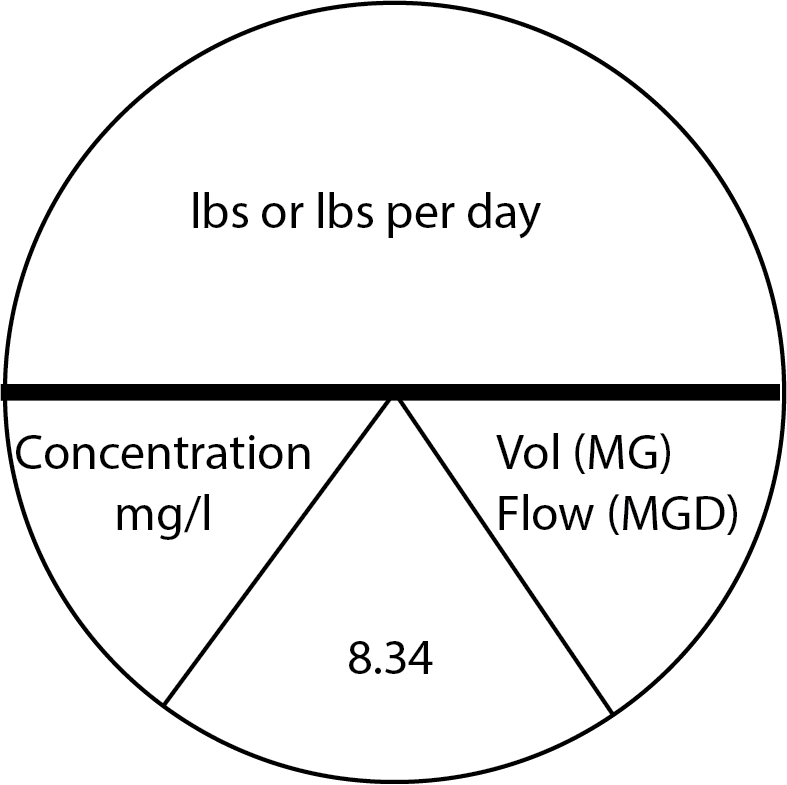
\includegraphics[scale=0.5]{PoundsFormula}
\end{center}

There are three variables – (lbs, concentration and volume) and one constant (8.34) in the pounds formula.  Knowing any of the two variables in the formula, one can calculate the third (unknown) variable by rearranging the equation.

\section{Concentration}\index{Concentration}

Concentration is typically expressed as mg/l which is the weight of the constituent (mg) in 1 l (liter) of solution (wastewater).  As 1 l of water weighs 1 million mg, a concentration of 1 mg/l implies 1 mg of constituent per 1 million mg of water or one part per million (ppm).   \textbf{Thus, mg/l and ppm are synonymous.}\\  
Sometimes the constituent concentration is expressed in terms of percentage.\\
\vspace{6pt}
For example:  sludge containing 5\% solids or a 12.5\% chlorine concentration solution.\\
\vspace{6pt}
As one liter of water weighs 1,000,000 mg, one percent of that weight is 10,000 mg.  So 1\% solids implies 10,000 mg of solids per liter or 10,000 mg/l or 10,000 ppm.\\
\vspace{6pt}
$1\% concentration = 10,000 \enspace ppm \enspace or \enspace\frac{mg}{l}$\\
$0.1\% concentration = 1,000 \enspace ppm \enspace or \enspace \frac{mg}{l}$\\
$0.01\% concentration = 100 \enspace ppm \enspace or \enspace \frac{mg}{l}$\\
$10\% concentration = 100,000 \enspace ppm \enspace or \enspace \frac{mg}{l}$\\
$5\% concentration = 50,000 \enspace ppm \enspace or \enspace \frac{mg}{l}$\\
$12.5\% concentration = 125,000 \enspace ppm \enspace or \enspace \frac{mg}{l}$

\subsection{Example Problems}
% \hl{Example Problems}\\

Problem 1\\Calculate the lbs/day of solids entering the plant given the influent flow is 5 MGD with an average solids concentration  of 250 mg/l.\\

Solution:\\

Applying lbs formula:\\
$\dfrac{lbs}{day}=5 MGD *250\dfrac{mg}{l}*8.34 = \boxed{10,425\dfrac{lbs}{day}}$
\\
Problem 2\\Calculate the lbs of solids in the primary sludge if the sludge flow is 7500 gallons and the solids concentration is 4.5\%.\\
Solution\\
Applying lbs formula:\\
$lbs \enspace solids = \dfrac{7500}{1,000,000}MG * 4.5*10,000 *8.34 = \boxed{2,815 \enspace lbs \enspace solids}$\\
\textbf{Note:}\\  
1) 7500 gallons was converted to MG by dividing by 1,000,000\\
$7500 \enspace gallons * \dfrac{1 MG}{1,000,000 \enspace gallon}$\\
2) 4.5\% was converted to mg/l by multiplying by 10,000 as 1\%=10,000mg/l

\newpage
\section{Area \& Volume}\index{Area \& Volume}
% \section{Area \& Volume}\index{Area \& Volume}

% \begin{snugshade*}
% 	\item \noindent\textsc{Area \& Volume}
% \end{snugshade*}

\begin{center}
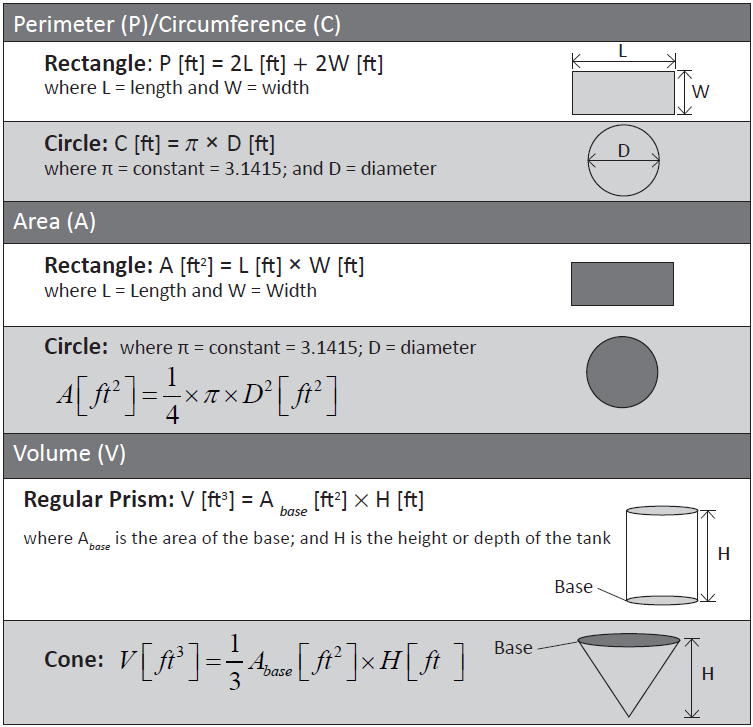
\includegraphics[scale=0.5]{Area&VolumeFormula}
\end{center}
\subsection{Example Problems}
% \hl{Example Problems}\\
\begin{enumerate}

\item The floor of a rectangular building is 20 feet long by 12 feet wide and the inside walls are 10 feet high. Find the total surface area of the inside walls of this building\\
Solution:\\
% \begin{center}
\begin{tikzpicture}
	%%% Edit the following coordinate to change the shape of your
	%%% cuboid
      
	%% Vanishing points for perspective handling
	\coordinate (P1) at (-7cm,1.5cm); % left vanishing point (To pick)
	\coordinate (P2) at (8cm,1.5cm); % right vanishing point (To pick)

	%% (A1) and (A2) defines the 2 central points of the cuboid
	\coordinate (A1) at (0em,0cm); % central top point (To pick)
	\coordinate (A2) at (0em,-2cm); % central bottom point (To pick)

	%% (A3) to (A8) are computed given a unique parameter (or 2) .8
	% You can vary .8 from 0 to 1 to change perspective on left side
	\coordinate (A3) at ($(P1)!.8!(A2)$); % To pick for perspective 
	\coordinate (A4) at ($(P1)!.8!(A1)$);

	% You can vary .8 from 0 to 1 to change perspective on right side
	\coordinate (A7) at ($(P2)!.7!(A2)$);
	\coordinate (A8) at ($(P2)!.7!(A1)$);

	%% Automatically compute the last 2 points with intersections
	\coordinate (A5) at
	  (intersection cs: first line={(A8) -- (P1)},
			    second line={(A4) -- (P2)});
	\coordinate (A6) at
	  (intersection cs: first line={(A7) -- (P1)}, 
			    second line={(A3) -- (P2)});

	%%% Depending of what you want to display, you can comment/edit
	%%% the following lines

	%% Possibly draw back faces

	\fill[gray!40] (A2) -- (A3) -- (A6) -- (A7) -- cycle; % face 6
	\node at (barycentric cs:A2=1,A3=1,A6=1,A7=1) {\tiny Floor=W*L};
	
	\fill[gray!50] (A3) -- (A4) -- (A5) -- (A6) -- cycle; % face 3
	\node at (barycentric cs:A3=1,A4=1,A5=1,A6=1) {\tiny Wall - W*H};
	
	\fill[gray!10, opacity=0.2] (A5) -- (A6) -- (A7) -- (A8) -- cycle; % face 4
	\node at (barycentric cs:A5=1,A6=1,A7=1,A8=1) {\tiny Wall - L*H};
	
	\fill[gray!10,opacity=0.5] (A1) -- (A2) -- (A3) -- (A4) -- cycle; % f2
	\node at (barycentric cs:A1=1,A2=1,A3=1,A4=1) {\tiny Wall - L*H};
	
	\fill[gray!40,opacity=0.2] (A1) -- (A4) -- (A5) -- (A8) -- cycle; % f5
	\node at (barycentric cs:A1=1,A4=1,A5=1,A8=1) {\tiny Ceiling=W*L};	
	
	\draw[thick,dashed] (A5) -- (A6);
	\draw[thick,dashed] (A3) -- (A6);
	\draw[thick,dashed] (A7) -- (A6);

	%% Possibly draw front faces

	%\fill[orange] (A1) -- (A8) -- (A7) -- (A2) -- cycle; % face 1
	\node at (barycentric cs:A1=1,A8=1,A7=1,A2=1) {\tiny Wall - W*H};
	


	%% Possibly draw front lines
	\draw[thick] (A1) -- (A2);

	\draw[<->] (-1.8,0.38) -- (-1.8,-1.3)node [midway, above=-1.8mm] {\hspace{-1.3cm}\tiny Height=10'};
	\draw[<->] (-1.6,-1.4) -- (-.3,-2.1)node [midway, above=-2.6mm] {\hspace{-1.3cm}\tiny Length=20'};
	\draw[<->] (2.6,-1.13) -- (0.2,-2.2)node [midway, below=.6mm] {\hspace{1.2cm}\tiny Width=12'};
	\draw[thick] (A3) -- (A4);
	\draw[thick] (A7) -- (A8);
	\draw[thick] (A1) -- (A4);
	\draw[thick] (A1) -- (A8);
	\draw[thick] (A2) -- (A3);
	\draw[thick] (A2) -- (A7);
	\draw[thick] (A4) -- (A5);
	\draw[thick] (A8) -- (A5);
	
	% Possibly draw points
	% (it can help you understand the cuboid structure)
%	\foreach \i in {1,2,...,8}
%	{
%	  \draw[fill=black] (A\i) circle (0.15em)
%	    node[above right] {\tiny \i};
%	}
	% \draw[fill=black] (P1) circle (0.1em) node[below] {\tiny p1};
	% \draw[fill=black] (P2) circle (0.1em) node[below] {\tiny p2};
\end{tikzpicture}\\
% \end{center}
2 Walls W*H + 2 Walls L*H= $2*12*10ft^2 + 2*20*10ft^2$\\
$=240+400=\boxed{640ft^2}$

2 Walls W*H + 2 Walls L*H + Floor + Ceiling= $2*12*10ft^2 + 2*20*10ft^2 + 2*12*20ft^2$\\
$=240+400+480=\boxed{1,120ft^2}$

\item How many gallons of paint will be required to paint the inside walls of a 40 ft long x 65 ft wide x 20 ft high tank if the paint coverage is 150 sq. ft per gallon.  Note:  We are painting walls only.  Disregard the floor and roof areas.
Solution:\\
\vspace{0.3cm}
% \begin{center}
\begin{tikzpicture}
	%%% Edit the following coordinate to change the shape of your
	%%% cuboid
      
	%% Vanishing points for perspective handling
	\coordinate (P1) at (-7cm,1.5cm); % left vanishing point (To pick)
	\coordinate (P2) at (8cm,1.5cm); % right vanishing point (To pick)

	%% (A1) and (A2) defines the 2 central points of the cuboid
	\coordinate (A1) at (0em,0cm); % central top point (To pick)
	\coordinate (A2) at (0em,-2cm); % central bottom point (To pick)

	%% (A3) to (A8) are computed given a unique parameter (or 2) .8
	% You can vary .8 from 0 to 1 to change perspective on left side
	\coordinate (A3) at ($(P1)!.8!(A2)$); % To pick for perspective 
	\coordinate (A4) at ($(P1)!.8!(A1)$);

	% You can vary .8 from 0 to 1 to change perspective on right side
	\coordinate (A7) at ($(P2)!.7!(A2)$);
	\coordinate (A8) at ($(P2)!.7!(A1)$);

	%% Automatically compute the last 2 points with intersections
	\coordinate (A5) at
	  (intersection cs: first line={(A8) -- (P1)},
			    second line={(A4) -- (P2)});
	\coordinate (A6) at
	  (intersection cs: first line={(A7) -- (P1)}, 
			    second line={(A3) -- (P2)});

	%%% Depending of what you want to display, you can comment/edit
	%%% the following lines

	%% Possibly draw back faces

	\fill[gray!40] (A2) -- (A3) -- (A6) -- (A7) -- cycle; % face 6
	\node at (barycentric cs:A2=1,A3=1,A6=1,A7=1) {};
	
	\fill[gray!50] (A3) -- (A4) -- (A5) -- (A6) -- cycle; % face 3
	\node at (barycentric cs:A3=1,A4=1,A5=1,A6=1) {\tiny Wall - W*H};
	
	\fill[gray!10, opacity=0.2] (A5) -- (A6) -- (A7) -- (A8) -- cycle; % face 4
	\node at (barycentric cs:A5=1,A6=1,A7=1,A8=1) {\tiny Wall - L*H};
	
	\fill[gray!10,opacity=0.5] (A1) -- (A2) -- (A3) -- (A4) -- cycle; % f2
	\node at (barycentric cs:A1=1,A2=1,A3=1,A4=1) {\tiny Wall - L*H};
	
	\fill[gray!40,opacity=0.2] (A1) -- (A4) -- (A5) -- (A8) -- cycle; % f5
	\node at (barycentric cs:A1=1,A4=1,A5=1,A8=1) {};	
	
	\draw[thick,dashed] (A5) -- (A6);
	\draw[thick,dashed] (A3) -- (A6);
	\draw[thick,dashed] (A7) -- (A6);

	%% Possibly draw front faces

	%\fill[orange] (A1) -- (A8) -- (A7) -- (A2) -- cycle; % face 1
	\node at (barycentric cs:A1=1,A8=1,A7=1,A2=1) {\tiny Wall - W*H};
	


	%% Possibly draw front lines
	\draw[thick] (A1) -- (A2);

	\draw[<->] (-1.8,0.38) -- (-1.8,-1.3)node [midway, above=-1.8mm] {\hspace{-1.3cm}\tiny Height=20'};
	\draw[<->] (-1.6,-1.4) -- (-.3,-2.1)node [midway, above=-2.6mm] {\hspace{-1.3cm}\tiny Length=45'};
	\draw[<->] (2.6,-1.13) -- (0.2,-2.2)node [midway, below=.6mm] {\hspace{1.2cm}\tiny Width=65'};
	\draw[thick] (A3) -- (A4);
	\draw[thick] (A7) -- (A8);
	\draw[thick] (A1) -- (A4);
	\draw[thick] (A1) -- (A8);
	\draw[thick] (A2) -- (A3);
	\draw[thick] (A2) -- (A7);
	\draw[thick] (A4) -- (A5);
	\draw[thick] (A8) -- (A5);
	
	% Possibly draw points
	% (it can help you understand the cuboid structure)
%	\foreach \i in {1,2,...,8}
%	{
%	  \draw[fill=black] (A\i) circle (0.15em)
%	    node[above right] {\tiny \i};
%	}
	% \draw[fill=black] (P1) circle (0.1em) node[below] {\tiny p1};
	% \draw[fill=black] (P2) circle (0.1em) node[below] {\tiny p2};
\end{tikzpicture}\\
% \end{center}
\vspace{0.3cm}
2 Walls W*H + 2 Walls L*H = $2*65*20ft^2 + 2*40*20ft^2= 2,600+1,600=4,200ft^2$\\
$\implies @150\dfrac{ft^2}{gal} \enspace paint \enspace coverage \enspace \rightarrow \enspace \dfrac{4,200\cancel{ft^2}}{150\dfrac{\cancel{ft^2}}{gal}}=\boxed{28 \enspace gallons}$
\vspace{0.3cm}
\item What is the circumference of a 100 ft diameter circular clarifier?\\
\vspace{0.3cm}
Solution:\\
\vspace{0.3cm}
$Circumference=\pi*D=3.14*100ft=\boxed{314ft}$
\vspace{0.3cm}
\item If the surface area of a clarifier is 5,025$ft^2$, what is its diameter?\\
\vspace{0.3cm}
Solution:\\
\vspace{0.3cm}
$Surface \enspace area=\dfrac{\pi}{4}*D^2 \enspace \implies 5025(ft^2)=0.785*D^2 (ft^2)$\\
$\implies D^2=\dfrac{5025}{0.785} \implies D=\sqrt{6401.3}=\boxed{80ft}$
\vspace{0.3cm}

\item How many gallons of wastewater would 600 feet of 6-inch diameter pipe hold, approximately?\\
\vspace{0.3cm}
Solution:\\

\vspace{0.3cm}
% \begin{center}
\begin{tikzpicture}
\draw (0,0) ellipse (0.1cm and 0.3cm);
\draw (10,0) ellipse (0.1cm and 0.3cm);
\draw [-] (0,-0.29) -- (10,-0.29);
\draw [-] (0,0.29) -- (10,0.29);
\draw [<->] (10,-0.28) -- (10,0.28) node [midway, below=-3mm] {\hspace{2.6cm}Diameter=6"};
\draw [<->] (0,-.68) -- (10,-.68)node [midway, below] {\hspace{0.9cm}Length=600'};
\end{tikzpicture}
% \end{center}
\vspace{0.3cm}
$Volume=\dfrac{\pi}{4}D^2*L=0.785*\Big(\dfrac{6}{12}\Big)^2*600\cancel{ft^3}*7.48\dfrac{gallons}{\cancel{ft^3}}=\boxed{881 \enspace gallons}$
\newpage
\item A 110 ft diameter digester with a 12 ft deep cone is operated at a side water depth of 20 ft.  Caluclate the volume of sludge in the digester in $ft^3$ and gallons.\\
\vspace{0.3cm}
Solution:\\
\vspace{0.3cm}
% \begin{center}
\begin{tikzpicture}
\draw (0,0) ellipse (2cm and 0.3cm);
\draw (0,-2.3) ellipse (2cm and 0.3cm);
\draw (0,-.8) ellipse (2cm and 0.3cm);
\draw [-] (2,-2.3) -- (2,0);
\draw [<->] (-2,0) -- (2,0) node [midway, below=-0.9cm] {\hspace{0.9cm}Diameter (D)=110'}; 
\draw [<->] (-2.6,-2.3) -- (-2.6,0) node [midway, below=-.3cm] {\hspace{-2.6cm}Cylinder Height};
\draw [<->] (2.5,-2.3) -- (2.5,-0.8) node [midway, below=-0.2cm] {\hspace{5.2cm}Side Water Depth (SWD) =20'};
\draw [-] (0,-4) -- (2,-2.3);
\draw [-] (0,-4) -- (-2,-2.3);
\draw [-] (0,-4) -- (2,-2.3);
\draw [-] (-2,0) -- (-2,-2.3);
\draw [<->] (2.5,-2.3) -- (2.5,-4)node [midway, below=-0.4cm] {\hspace{3.8cm}Cone Depth (CD)=12'};
\end{tikzpicture}\\
% \end{center}
$Digester \enspace volume=Volume_{cylinder}+Volume_{cone}$\\
$\implies Digester \enspace volume=\dfrac{\pi}{4}D^2*SWD+\dfrac{1}{3}*\Bigg(\dfrac{\pi}{4}*D^2*CD\Bigg)$\\
\vspace{0.3cm}
$=0.785*110^2*20+1.05*110^2*12=\boxed{227,988ft^3}$\\
\vspace{0.3cm}
$227,988\cancel{ft^3}*7.48\dfrac{gallons}{\cancel{ft^3}}=\boxed{1,705,352 \enspace gallons}$
\end{enumerate}

\section{Process Removal Efficiency}\index{Process Removal Efficiency}

% \section{Process Removal Efficiency}\index{Process Removal Efficiency}
% \begin{snugshade*}
% 	\item \noindent\textsc{Process Removal Efficiency}
% \end{snugshade*}
\begin{itemize}
\item Process removal rate or removal efficiency is the percentage of the inlet concentration removed.  
\item It is used for quantifying the pollutant removal during wastewater treatment and is established based upon the amount of a particular wastewater constituent entering and leaving a treatment process.

\item $Process \enspace Removal \enspace Rate \enspace (\%) = \dfrac{Pollutant \enspace  In-Pollutant\enspace  Out}{Pollutant \enspace In}*100$\\

\item If 10 units of a pollutant are entering a process and 8 units of pollutant are leaving (process removes 2 units), then the process removal rate for that pollutant is (10-8)/10*100=20\%.  In this example the process is 20\% efficient in removing that particular pollutant.

\item The amount of pollutant can be measured in terms of concentration (mg/l) or in terms of mass loading (lbs).  The pounds formula is used for calculating the mass loadings.  
\end{itemize}
The above example is for calculating the removal efficiency using the inlet and outlet concentrations or mass loading.\\
The methods below can be used for calculating either the inlet or outlet pollutant concentrations, if the removal efficiency and the corresponding inlet or outlet concentrations are given. 


\hl{Case 1:  Calculating outlet conc. (X) given the inlet conc. and removal efficiency (RE\%):}

\tikzstyle{block} = [rectangle, draw, fill=red!40, 
    text width=6em, text centered, rounded corners, minimum height=3em]
\tikzstyle{arrow} = [draw, -latex']
\begin{figure}[!h]
\centering
\begin{tikzpicture}[node distance =1.5cm, auto]
    \draw ++(0,0) node [block] (Process) {Process};
   \node[node distance=1.9in] (dummy_in) [left of=Process] {In};
   \node[node distance=1.9in] (dummy_out) [right of=Process] {Out};
	\node (Removal) [below of=Process, yshift=-0in] {${Removal \enspace Efficiency=RE\% \enspace (Given)}$};
    \path [arrow] (dummy_in)-- (Process)  node [above] {\hspace{-5.8cm}$A \enspace mg/l \enspace (Given) $} node [below] {\hspace{-5.8cm}$100 \enspace mg/l$};
    \path [arrow] (Process) -- (dummy_out)  node [above] {\hspace{-4cm}$X \enspace mg/l \enspace (Unknown)$} node [below] {\hspace{-3.9cm}($100-RE\%)\enspace mg/l$};
   \draw[arrow] (Process) -- (Removal);
\end{tikzpicture}
\end{figure}
Using the fact that if the inlet concentration was 100 mg/l, the outlet concentration would be 100 minus the removal efficiency.\\
Setup the equation as:  $\dfrac{Out}{In}: \enspace \dfrac{X \enspace mg/l}{A \enspace mg/l}=\dfrac{100-RE\%}{100}$\\
Calculate X using cross multiplication - if $\dfrac{A}{B}=\dfrac{C}{D} \implies A=B*\dfrac{C}{D}$:\\
$X \enspace mg/l=A \enspace mg/l*\dfrac{100-RE\%}{100}$\\


\hl{Case 2:  Calculating inlet conc. (X) given the outlet conc. and removal efficiency (RE\%):}

\begin{figure}[!h]
\centering
\begin{tikzpicture}[node distance =1.5cm, auto]
    \draw ++(0,0) node [block] (Process) {Process};
   \node[node distance=1.9in] (dummy_in) [left of=Process] {In};
   \node[node distance=1.9in] (dummy_out) [right of=Process] {Out};
	\node (Removal) [below of=Process, yshift=-0in] {$Removal \enspace Efficiency=RE\% \enspace (Given)$};
    \path [arrow] (dummy_in)-- (Process)  node [above] {\hspace{-5.8cm}$X \enspace mg/l \enspace (Unknown)$} node [below] {\hspace{-5.8cm}$100 \enspace mg/l$};
    \path [arrow] (Process) -- (dummy_out)  node [above] {\hspace{-4cm}$A \enspace mg/l \enspace (Given)$} node [below] {\hspace{-3.9cm}($100-RE\%)\enspace mg/l$};
   \draw[arrow] (Process) -- (Removal);
\end{tikzpicture}
\end{figure}
Using the fact that if the inlet concentration was 100 mg/l, the outlet concentration would be 100 minus the removal efficiency.\\
Setup the equation as:  $\dfrac{In}{Out}: \enspace \dfrac{X \enspace mg/l}{A \enspace mg/l}=\dfrac{100}{100-RE\%}$\\
\vspace{0.3cm}
Calculate X using cross multiplication - if $\dfrac{A}{B}=\dfrac{C}{D} \implies A=B*\dfrac{C}{D}$:\\
$X \enspace mg/l=A \enspace mg/l*\dfrac{100}{100-RE\%}$\\

\vspace{0.4cm}
\subsection{Example Problems}
% \hl{Example Problems:}\\

\begin{enumerate}

\item What is the \% removal efficiency if the influent concentration is 10 mg/L and the effluent concentration is 2.5 mg/L?\\
$Removal \enspace Rate (\%) = \dfrac{In-Out}{In}*100 \implies \dfrac{10-2.5}{10}*100=\boxed{75\%}$



\item Calculate the outlet concentration if the inlet concentration is 80 mg/l and the process removal efficiency is 60\%\\
Solution:\\

\tikzstyle{block} = [rectangle, draw, fill=red!40, 
    text width=6em, text centered, rounded corners, minimum height=3em]
\tikzstyle{arrow} = [draw, -latex']
\begin{figure}[!h]
\centering
\begin{tikzpicture}[node distance =1.5cm, auto]
    \draw ++(0,0) node [block] (Process) {Process};
   \node[node distance=1.5in] (dummy_in) [left of=Process] {In};
   \node[node distance=1.5in] (dummy_out) [right of=Process] {Out};
	\node (Removal) [below of=Process, yshift=-0in] {$Removal \enspace Efficiency=60\%$};
    \path [arrow] (dummy_in)-- (Process)  node [above] {\hspace{-4.39cm}$80mg/l$} node [below] {\hspace{-4.39cm}$100mg/l$};
    \path [arrow] (Process) -- (dummy_out)  node [above] {\hspace{-3.cm}$Xmg/l$} node [below] {\hspace{-3cm}40mg/l};
   \draw[arrow] (Process) -- (Removal);
\end{tikzpicture}
%\caption[MFCC]{Diagrama en bloques del cálculo de las MFCC para un frame.}
%\label{MFCC}
\end{figure}

$\dfrac{Out}{In} \enspace:\enspace\dfrac{Actual \enspace Outlet (X)}{80}=\dfrac{100-60}{100}$\\
$\implies \dfrac{Actual \enspace Outlet (X)}{80} =0.4$\\
$\implies Actual \enspace  Outlet (X) = 0.4 * 80 = \boxed{32 mg/l}$\\


\item Calculate the inlet concentration if the outlet concentration is 80 mg/l and the process removal efficiency is 60\%\\

\tikzstyle{block} = [rectangle, draw, fill=red!40, 
    text width=6em, text centered, rounded corners, minimum height=3em]
\tikzstyle{arrow} = [draw, -latex']
\begin{figure}[!h]
\centering
\begin{tikzpicture}[node distance =1.5cm, auto]
    \draw ++(0,0) node [block] (Process) {Process};
   \node[node distance=1.5in] (dummy_in) [left of=Process] {In};
   \node[node distance=1.5in] (dummy_out) [right of=Process] {Out};
	\node (Removal) [below of=Process, yshift=-0in] {$Removal \enspace Efficiency=60\%$};
    \path [arrow] (dummy_in)-- (Process)  node [above] {\hspace{-4.39cm}$Xmg/l$} node [below] {\hspace{-4.39cm}$100mg/l$};
    \path [arrow] (Process) -- (dummy_out)  node [above] {\hspace{-3.cm}80mg/l} node [below] {\hspace{-3cm}40mg/l};
   \draw[arrow] (Process) -- (Removal);
\end{tikzpicture}
\end{figure}

$\dfrac{In}{Out} \enspace : \enspace \dfrac{Actual \enspace inlet \enspace  (X)}{80}=\dfrac{100}{100-60}\implies \dfrac{Actual \enspace inlet \enspace  (X)}{80}=2.5$\\    
Rearranging the equation:   $Actual \enspace inlet (X)=2.5*80 = \boxed{200 mg/l}$\\

\item If a plant removes 35\% of the influent BOD in the primary treatment and 85\% of the remaining BOD in the secondary system, what is the BOD of the raw wastewater if the BOD of the final effluent is 20mg/l\\
Solution:\\

\begin{figure}[!h]
\centering
\begin{tikzpicture}[node distance =1.5cm, auto]
    \draw ++(0,0) node [block] (Primary) {Primary};
    
   \node[node distance=1.9in] (dummy_in) [left of=Primary] {Influent BOD};
   \node[node distance=1.9in] (dummy_out) [right of=Primary] {Primary BOD Out};
	\node (Removal) [below of=Primary, yshift=-0in] {$Removal \enspace Efficiency=35\% $};
    \path [arrow] (dummy_in)-- (Primary)  node [above] {\hspace{-4.8cm}$X \enspace mg/l \enspace$} node [below] {};
    \path [arrow] (Primary) -- (dummy_out)  node [above] {\hspace{-4.9cm}$0.65X \enspace mg/l$} node [below] {};
   \draw[arrow] (Process) -- (Removal);
\end{tikzpicture}
\end{figure}


\begin{figure}[!h]
\centering
\begin{tikzpicture}[node distance =1.5cm, auto]
    \draw ++(0,0) node [block] (Secondary) {Secondary};
    
   \node[node distance=1.9in] (dummy_in) [left of=Secondary] {Primary BOD Out};
   \node[node distance=1.9in] (dummy_out) [right of=Secondary] {Secondary BOD Out};
	\node (Removal) [below of=Secondary, yshift=-0in] {$Removal \enspace Efficiency=85\% $};
    \path [arrow] (dummy_in)-- (Secondary)  node [above] {\hspace{-4.8cm}$0.65X \enspace mg/l \enspace$} node [below] {\hspace{-5cm}$100 \enspace mg/l$};
    \path [arrow] (Secondary) -- (dummy_out)  node [above] {\hspace{-4.9cm}$20 \enspace mg/l$} node [below] {\hspace{-4.9cm}$15 \enspace mg/l$};
   \draw[arrow] (Process) -- (Removal);
\end{tikzpicture}
\end{figure}
\vspace{0.3cm}
For the Secondary process:\\
$\dfrac{In}{Out}: \enspace \dfrac{0.65X}{20}=\dfrac{100}{15} \implies X \enspace mg/l=\dfrac{100*20}{15*0.65}=\boxed{205 \enspace mg/l}$\\

\vspace{0.3cm}
Alternate Solution \#1

$\xrightarrow[
				\text{X}\dfrac{mg}{l}
			]
			{
			\text{Influent BOD}
			}
 \boxed{Primary}
 \xrightarrow[
 				\text{X-0.35X=X*(1-0.35)=0.65X}\dfrac{mg}{l}
 			]
 			{
 			\text{Primary Effluent BOD}
 			}
 \boxed{Secondary}
 \xrightarrow[
				\text{0.65X-0.5525X=(0.65-0.5525)X=0.0975X }
			 ]
			{
			\text{Secondary Effluent BOD}
			}
$\\
\hspace{2.8cm}$\downarrow$ {\tiny(0.35X)BOD Removed}\hspace{3.2cm}$\downarrow$ {\tiny(0.65*0.85)X = 0.5525X BOD Removed}\\
$\implies 0.0975X=20 \implies X=\dfrac{20}{0.0975}=\boxed{205\dfrac{mg}{l}}$\\

\vspace{0.3cm}

Alternate Solution \#2:\\
$\xrightarrow[\text{X}\dfrac{mg}{l}]{\text{Influent BOD}}\boxed{Primary}\xrightarrow[\text{0.65X}]{\text{Primary Effluent BOD}}\boxed{Secondary}\xrightarrow[\text{(0.65*0.15)X}]{\text{Secondary Effluent BOD}}$\\
\hspace{2.8cm}$\downarrow$ {\tiny(0.35X)BOD Removed}\hspace{2.2cm}$\downarrow$ {\tiny(0.65X*0.85)BOD Removed}\\

Primary Effluent BOD = Influent BOD * (1-Primary BOD Removal), and\\
Secondary Effluent BOD=[Primary Effluent BOD]*(1-Secondary BOD Removal)\\
Secondary Eff. BOD=[Influent BOD * (1-Primary BOD Removal)]*(1-Secondary BOD Removal)\\

Therefore, 20 = [X*(1-0.35)] * (1-0.85)= X*0.65*0.15\\
$\implies 20 \enspace \dfrac{mg}{l}= 0.0975X \implies X=\dfrac{20}{0.0975}=\boxed{205 \enspace \dfrac{mg}{l}}$

\end{enumerate}
\section{Pumping}\index{Pumping}
% \section{Pumping}\index{Pumping}
% \pagebreak
% \begin{snugshade*}
% 	\item \noindent\textsc{Pumping}
% \end{snugshade*}
For Grades I \& II, pumping rate problems include the following:
% \begin{enumerate}
% \definecolor{shadecolor}{RGB}{225, 235, 235}
% \begin{snugshade*}
% \item \noindent\textsc{Calculating volume pumped in a given time interval given the pump flow rate\\}
% \end{snugshade*}
\subsection{Calculating volume pumped given the pump flow rate}\index{Calculating volume pumped given the pump flow rate}

\textbf{Method:\\}
\hspace{1cm}Step 1. Multiply the pump flow rate by the time interval\\
\textbf{Make sure:}
\begin{itemize}
\item The time units - in the given time interval and in the pump flow rate match
\end{itemize}
\subsection{Calculating time to pump a certain volume}\index{Calculating time to pump a certain volume}
% \begin{snugshade*}
% \item \noindent\textsc{Calculating time to pump a certain volume given the pump flow rate\\}
% \end{snugshade*}
\textbf{Method:}
\hspace{1cm}Step 1. Calculate the total volume pumped\\
\hspace{1cm}Step 2.	Divide the total volume by the pump flow rate\\
\textbf{Make sure:}
\begin{itemize}
\item The volume units - in the volume that needs to be pumped and in the pump flow rate match
\item The time unit in the pump flow rate needs to be converted to the time unit that you need the answer in
\end{itemize}
% \end{enumerate}

\section{Example Problems}
% \hl{Example Problems:}\\

\begin{enumerate}

\item A sludge pump is set to pump 5 minutes each hour. It pumps at the rate of 35 gpm. How many gallons of sludge are pumped each day?\\
Solution:\\
$\dfrac{35 \enspace gal \enspace sludge}{\cancel{min}}*\dfrac{5 \enspace \cancel{min}}{\cancel{hr}} *\dfrac{24 \enspace \cancel{hr}}{day}=\boxed{\dfrac{4,200 \enspace gallons}{day}}$\\
\vspace{0.5cm}

\item A sludge pump operates 5 minutes each 15 minute interval.  If the pump capacity is 60 gpm, how many gallons of sludge are pumped daily?

$\dfrac{60 \enspace gal \enspace sludge}{\xcancel{min}}*\dfrac{5 \enspace \xcancel{min}}{15 \enspace \cancel{min}}*1440\dfrac{\cancel{min}}{day}=\boxed{\dfrac {28,800 \enspace gal \enspace sludge }{day}}$\\

\item Given the tank is 10ft wide, 12 ft long and 18 ft deep tank including 2 ft of freeboard when filled to capacity. How much time (minutes) will be required to pump down this tank to a depth of 2 ft when the tank is at maximum capacity using a 600 GPM pump\\
Solution:\\
\vspace{0.5cm}


\begin{tikzpicture}

\pgfmathsetmacro{\cubexx}{4}
\pgfmathsetmacro{\cubeyy}{1.5}
\pgfmathsetmacro{\cubezz}{2}
\pgfmathsetmacro{\cubex}{4}
\pgfmathsetmacro{\cubey}{0.5}
\pgfmathsetmacro{\cubez}{2}
\pgfmathsetmacro{\cubexxx}{4}
\pgfmathsetmacro{\cubeyyy}{4}
\filldraw [fill=cyan!10!white, draw=black] (0,-\cubey,0) -- ++(-\cubexx,0,0) -- ++(0,-\cubeyy,0) -- ++(\cubexx,0,0) -- cycle ;
\filldraw [fill=cyan!0!white, draw=black] (0,-\cubey,0) -- ++(0,0,-\cubezz) -- ++(0,-\cubeyy,0) -- ++(0,0,\cubezz) -- cycle;
\filldraw [fill=cyan!10!white, draw=black] (0,-\cubey,0) -- ++(0,0,-\cubezz) -- ++(0,-\cubeyy,0) -- ++(0,0,\cubezz) -- cycle;
%\filldraw [fill=cyan!10!white, draw=black] (0,-\cubey,0) -- ++(-\cubexx,0,0) -- ++(0,0,-\cubezz) -- ++(\cubexx,0,0) -- cycle;
%%%\draw (0,-0.5,0) -- ++(-\cubex,0,0) -- ++(0,-\cubey,-\cubez) -- ++(\cubex,0,0) -- cycle;
\draw (-\cubex,0,0) -- ++(0,0,-\cubez) -- ++(0,-\cubey,0) -- ++(0,0,\cubez) -- cycle;
\draw (0,-\cubey,0) -- ++(-\cubex,0,0) -- ++(0,0,-\cubez) -- ++(\cubex,0,0) -- cycle;
\filldraw [fill=white, draw=black] (0,0,0) -- ++(-\cubex,0,0) -- ++(0,-\cubey,0) -- ++(\cubex,0,0) -- cycle ;
\filldraw [fill=white, draw=black] (0,0,0) -- ++(0,0,-\cubez) -- ++(0,-\cubey,0) -- ++(0,0,\cubez) -- cycle;
\filldraw [fill=white, draw=black] (0,0,0) -- ++(0,0,-\cubez) -- ++(0,-\cubey,0) -- ++(0,0,\cubez) -- cycle;
\filldraw [fill=white, draw=black] (0,0,0) -- ++(-\cubex,0,0) -- ++(0,0,-\cubez) -- ++(\cubex,0,0) -- cycle;

%\filldraw [fill=RoyalBlue!10!white, draw=black] (0,-1.5,0) -- ++(-\cubex,0,0) -- ++(0,-\cubey,0) -- ++(\cubex,0,0) -- cycle ;

%\filldraw [fill=RoyalBlue!10!white, draw=black] (0,-1.5,0) -- ++(0,0,-\cubez) -- ++(0,-\cubey,0) -- ++(0,0,\cubez) -- cycle;



%%\draw (0,-0.5,0) -- ++(-\cubex,0,0) -- ++(0,0,-\cubez) -- ++(\cubex,0,0) -- cycle;
%%\filldraw [fill=white, draw=black] (-\cubex,0,0) -- ++(0,0,-\cubez) -- ++(0,-\cubey,0) -- ++(0,0,\cubez) -- cycle;
%%\filldraw [fill=white, draw=black] (0,-\cubey,0) -- ++(-\cubex,0,0) -- ++(0,0,-\cubez) -- ++(\cubex,0,0) -- cycle ;

\draw [<->] (-4,-2.3) -- (0,-2.3) node [midway, below] {12' Long};
\draw [<->] (1,-1.3) -- (1,.2) node [midway, midway] {\hspace{4.5cm}16' Water Depth (Initial)};
\draw [<->] (0.4,-1.62) -- (0.4,-1.1) node [midway, midway] {\hspace{-4.8cm} 2' Water Depth (Final)};
\draw [<->] (1,.8) -- (1,.2) node [midway, midway] {\hspace{2.4cm}2' Freeboard};
\draw [<->] (1,-1.3) -- (0,-2.3) node [midway, midway] {\hspace{2.3cm}10' Wide};
\end{tikzpicture}\\
Volume to be pumped=$12 \enspace ft*10 \enspace ft *(16-2)\enspace ft=1,680ft^3$\\
\vspace{0.3cm}
$\implies \dfrac{1,680\cancel{ft^3}*7.48\dfrac{\cancel{gal}}{\cancel{ft^3}}}{600\dfrac{\cancel{gal}}{min}}=\boxed{21min}$
\end{enumerate}

\chapterimage{TitleIII.png} % Chapter heading image

\chapter{Wastewater Constituents and Analysis}
% \begin{enumerate}[1.]
% 	\definecolor{shadecolor}{RGB}{200, 200, 240}

% 	%%%%%%%%%%%
% 	% LEVEL 2 %
% 	%%%%%%%%%%%

% 	\begin{snugshade*}
% 		\item \noindent\textsc{Wastewater Constituents}%$$$$$$$$$$$$$$$$$$$$%
% 	\end{snugshade*}
% 	Solids, organic matter, nutrients, pathogens and oil \& grease are the main target constituents of wastewater treatment operations.
% 	\begin{enumerate}[A.]%___________%
% 			\definecolor{shadecolor}{RGB}{225, 235, 235}

				%%%%%%%%%%%
				% LEVEL 3 %
				%%%%%%%%%%%
		% \begin{snugshade*}
		% 	\item \noindent\textsc{Organic Matter}%###############################%
		% \end{snugshade*}
		
		\section{Organics}\index{Organics}		
		\begin{itemize}
			\item The main reason for treating domestic wastewater is to remove the organic matter.  
			\item Organics are substances containing carbon, hydrogen and oxygen, and some of which may be combined with nitrogen, sulfur or phosphorous.
			\item About 50 percent of the solids present in wastewater are organic.  This fraction is generally of animal or vegetable life, dead animal matter, plant tissue or organisms, and also include synthetic organic compounds.
			\item The principal organic compounds present in domestic wastewater are proteins, carbohydrates and fats together with the products of their decomposition.
			\item Organics are subject to decay or decomposition through the activity of bacteria and other living organisms.  \hl{Since the organic fraction can be driven off at high temperatures, they are also called \textbf{volatile solids}}.\
			\item \emph{Organics in wastewater is typically quantified in terms of oxygen required to oxidize the carbon based material present} in wastewater using the following methods:\\
\subsection{Biochemical Oxygen Demand (BOD)}\index{Biochemical Oxygen Demand (BOD)}

			  %     \begin{enumerate}[i.]
			  %     	\definecolor{shadecolor}{RGB}{220,220,220}
					% %%%%%%%%%%%
					% % LEVEL 4 %
					% %%%%%%%%%%%
			  %     	\begin{snugshade*}
			  %     		\item \noindent\textsc{Biochemical Oxygen Demand (BOD)}%@@@@@@@@@@@@@@@@@@%
			  %     	\end{snugshade*}					
			      	\begin{itemize}
			      		\item The BOD of wastewater is measured in terms of oxygen required for the microorganisms to consume the organic material present.
			      		\item BOD is typically measured as BOD$_5$ which is the oxygen demand of the wastewater measured after 5 days of the initiation of the test.
			      		\item The test involves incubating a known dilution of wastewater in a 300 ml bottle for 5 days at 20\si{\degree}C.  The dissolved oxygen (DO) content at the start and end of the incubation period is used for calculating the BOD.
			      		\item For the test to be considered valid, the following criteria need to be met: 1) DO consumption during the test must be at least 2 mg/l, 2) DO remaining at the end of the test must be at least 1 mg/l, and 3) DO consumed in blank should be 0.2 mg/l or less
			      		      			
			      		\item BOD is a parameter to measure the strength of wastewater and the measurement of the wastewater treatment plant or treatment process influent and effluent BOD is standard practice to measure its performance.  Typical domestic wastewater BOD is about 200-250 mg/l.
			      		\item The oxygen consumed by the microorganisms during the BOD test is primarily for: 1) Oxidizing the carbonaceous material (cBOD – carbonaceous BOD), and 2) Oxidizing nitrogenous constituents such as ammonia (nBOD – nitrogenous BOD).
			      		\item Thus, BOD (Total) = cBOD + nBOD.  The cBOD and nBOD is measured by adding certain chemical inhibitors which will inhibit the bacteria responsible for consuming the nitrogenous matter, thus measuring only the cBOD as part of the BOD test.
			      		\item Since not all of the organics is metabolized in the 5 days of the regular BOD test, certain wastewater discharge permits require reporting of the ultimate BOD value (BOD$_U$)\\
			      	\end{itemize}

			    \subsection{Chemical Oxygen Demand (COD)}\index{Chemical Oxygen Demand (COD)}
			      	% \begin{snugshade*}
			      	% 	\item \noindent\textsc{Chemical Oxygen Demand (COD)}%@@@@@@@@@@@@@@@@@@%
			      	% \end{snugshade*}		  
			      	\begin{itemize}
			      		\item The COD test involves using chemical oxidizers to measure the oxygen demand of the wastewater.
			      		\item As the chemical oxidizers will oxidize other constituents present, including inorganic matter, the COD value of wastewater will be higher than the BOD.  
			      		\item The COD test can be conducted rather quickly than the 5 day BOD test, it is an effective method to quantify the wastewater strength and process efficiencies and allow operators to make timely process adjustments.
			      	\end{itemize}

			    \subsection{Total Organic Carbon (TOC)}
			      	% \begin{snugshade*}
			      	% 	\item \noindent\textsc{Total Organic Carbon (TOC):}\\%@@@@@@@@@@@@@@@@@@%
			      	% \end{snugshade*}
			      	The TOC method utilizes laboratory analytical instruments which directly measure the organic carbon content by quantifying the amount of carbon dioxide produced from the complete combustion of the organics present.
			      % \end{enumerate}
		\end{itemize}
		
		
		
			\hl{Note: BOD measures the amount of oxygen required by the microorganisms present to consume the organic material while COD measures the chemical oxidation required to oxidize all chemicals including organics present in wastewater.  BOD value of typical domestic sewage is about 200 - 250 mg/l while the COD value ranges from 300 - 450 mg/l.  Typical BOD:COD ratio ranges from 0.5-0.8.}\\


\section{Solids}\index{Solids}
% 		\pagebreak
% 				\begin{snugshade*}
% 			\item \noindent\textsc{Solids}
% 		\end{snugshade*}	
		Like BOD, wastewater solids is another critical parameter for establishing the wastewater strength and determining treatment process efficiencies. 
		\begin{itemize}
			\item The \texthl{solids can be classified as suspended or dissolved} based upon its ability to pass through a standardized filter paper.
			\item When the wastewater is filtered:
			      \begin{itemize}
			      	\item the residual solids remaining on the filter paper after drying in an oven at 103\si{\degree}C is the \hl{suspended solids} portion, and 
			      	\item the solids remaining after drying the filtrate are the \hl{dissolved solids}.
			      \end{itemize}
			\item Suspended solids include larger floating particles and consist of sand, grit, clay, fecal matter, paper, pieces of wood, particles of food and garbage, and similar materials.
			\item Suspended solids can be categorized based upon its settling characteristics as:
			      \begin{itemize}
			      	\item \hl{Settleable}
			      	\item \hl{Non-settleable}
			      	      \begin{itemize}
			      	      	\item \hl{Colloidial}-small, charged (typically negative) particles which do not settle easily.  Some of the colloidial particles are small enough to pass through the filter paper used for filtering the suspended solids
			      	      	\item \hl{Floatable}-example oil and grease and small plastics
			      	      \end{itemize}
			      \end{itemize}
			\item Dissolved solids in wastewater include organics.  However, the major elements of dissolved solids are inorganic ions such as Ca$^{+2}$, Mg$^{+2}$, Cl$^-$, SO$_4$ $^{-2}$ , HCO$_3$ $^-$, Fe$^{+2}$, PO$_4$ $^{-3}$, NO$_3$ $^-$.  These ions are part of the dissolved salts such as sodium chloride (NaCl), calcium bicarbonate (Ca(HCO$_3$)$_2$), magnesium phosphate (Mg$_3$PO$_4$) and others which are normally present in water and wastewater. 
			      \begin{itemize}
			      	\item Conductivity or electrical conductance (EC) measurement is typically conducted as the wastewater enters the plant as \hl{conductivity provides an indirect and simple measure of the amount of dissolved solids present.}  
			      	\item Conductivity or electrical conductance (EC) is a measure the amount of electrical current that can be conducted by a solution.  
			      	\item The conductance of electricity in a solution is due to the presence of dissolved inorganic ions 
			      	\item The higher the concentration of these ions, the higher is the conductivity. 
			      	\item \underline{Conductivity is measured in the units of mhos/cm or Siemens/cm.}  (Note:  mhos is the reverse of ohm which is a measure of resistance).
			      	\item Typical wastewater conductivities range from 50 to 1500 S/cm
			      \end{itemize}
			\item Both suspended and dissolved solids can be either \hl{volatile (organic)} or \hl{fixed (inorganic)}.
			\item \hl{Total Solids is thus a sum of TSS and dissolved solids or volatile and fixed solids.}
			      \begin{itemize}
			      	\item The volatile solids are typically of plant or animal origin .
			      	\item The fixed solids include sand, gravel and silt as well as the dissolved salts.
			      \end{itemize}
			      \begin{minipage}{0.5\textwidth}
			      	\item The volatile or fixed fractions are quantified by incinerating the solids in a muffler furnace at 550\si{\degree} which removes only the volatile solids leaving only the fixed solids behind.
			      	\item In terms of the size of the solids, the distribution is approximately thirty percent suspended and about seventy percent dissolved solids - which includes the colloidal particles which have passed through the filter paper.\\ 
			      	\item As primary treatment process involve settling of solids, establishing the settleable portion of the suspended solids is important.\\  
			      	\item \hl{The settleable solids are quantified using an Imhoff cone and are reported in ml/L}.  Imhoff cone is a 1 liter, clear cone shaped container, with volume graduations (ml) at the bottom.
			      						
			      \end{minipage}	
			      \begin{minipage}{0.5\textwidth}
			      	\begin{center}
			      		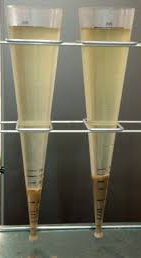
\includegraphics[scale=0.7]{ImhoffCone}\\
			      		Imhoff Cone\\
			      		\textit{Note the ml markings at the bottom of the cone}
			      		
			      		
			      	\end{center}
		      \end{minipage}
%			      \end{minipage}
			      	\item One factor which affects settleability is the conveyance time of the sewage to the treatment plant. 			
			      	\item The settleable component of the suspended solids will decrease as the sewage becomes more septic due to longer conveyance times.
			\item Influent and effluent total suspended solids are measured to establish the overall treatment and individual process efficiencies.  
			\item Volatile solids measurements before and after biological processes such as secondary treatment and digestion provide information on the process efficiency.\\
		\end{itemize}


	\subsection{Procedures for Solids Analysis}\index{Procedures for Solids Analysis}
% 		\begin{enumerate}%$$$$$$$$$$$$$$$$$$$$%
% 			\definecolor{shadecolor}{RGB}{220, 220, 220}
% 			\begin{snugshade*}
% 				\item \noindent\textsc{Procedures for Solids Analysis}
% 			\end{snugshade*}		
	\subsubsection{Determining wastewater suspended solids - Total(TSS) and Volatile(VSS) concentrations}\index{Determining wastewater suspended solids - Total(TSS) and Volatile(VSS) concentrations}			
			% \begin{enumerate}[a.]
			% 	\definecolor{shadecolor}{RGB}{110, 192, 221}
			% 	\begin{snugshade*}
			% 		\item \noindent\textsc{Determining wastewater suspended solids - Total(TSS) and Volatile(VSS) concentrations:}
			% 	\end{snugshade*}
				 
				%\hl{How total suspended solids concentration is established for a wastewater sample:}
				\begin{itemize}
					\item A known volume of wastewater sample is filtered through a pre-weighed filter paper
					\item The suspended solids will be retained by the filter
					\item The water with the dissolved solids will pass through the filter
					\item The filter paper with the filter solids is rinsed with distilled water to remove 
					\item The filter paper with the solids is dried in the oven and then weighed
					\item The difference between the weight of the dried filter paper with the solids and the pre-weighed filter paper, measured in mg, will be the suspended solids in: mg per the original quantity of wastewater sample taken.  This value can be converted to give the suspended solids content in mg/l
					\item A filter paper with the dried solids is incinerated in a muffler furnace
					\item The difference in the weight of the solids, before and after incineration is the fixed solids
					\item The difference between the weight of the solids before incineration and the fixed solids is the volatile solids
				\end{itemize}
				
	\subsubsection{Determining wastewater and sludge total solids (TS) and volatile solids (VS) concentrations}\index{Determining wastewater and sludge total solids (TS) and volatile solids (VS) concentrations}				
				
				% \begin{snugshade*}
				% 	\item \noindent\textsc{Determining wastewater and sludge total solids (TS) and volatile solids (VS) concentrations:}
				% \end{snugshade*}
				\begin{itemize}
					\item A certain quantity of wastewater (by volume) or sludge (by weight) is taken in a pre-weighed dish and weighed.  Note:  the sample is not filtered.
					\item The dish with the sample is dried in an oven
					\item The difference in the weight of the pre-weighed dish from that of the dish with the dried sample is the total solids
					\item The dried solids are incinerated in a muffler furnace
					\item The difference in the weight of the solids, before and after incineration is the fixed solids
					\item The difference between the fixed solids and the total solids is the volatile solids
					\item Total solids of a sludge sample is reported as a \% of the sludge weight.  A 7\% sludge has 7 lbs of solids for every 100 lbs of sludge.
				\end{itemize}
				
							
				
				
					\hl{For sludge samples, volatile solids is typically reported as the volatile solids fraction in \% of the total solids content of the sludge.  For example, if a 8\% sludge (i.e sludge which has 8\% TS or 80,000mg/l solids), is reported to have 70\% volatile, it means that 70\% of the total solids - 0.7*8\%=5.6\% or 56,000mg/l is the sludge volatile solids content.  \emph{70\% volatile does not meet the sludge has 700,000mg/l volatile solids}}\\
				
% 			\end{enumerate}
	\subsection{Summary of Wastewater Solids}\index{Summary of Wastewater Solids}		
% 			\begin{snugshade*}
% 				\item \noindent\textsc{Summary of Wastewater Solids}
% 			\end{snugshade*}
			\begin{itemize}
				\item Solids in wastewater can be categorized as dissolved or suspended
				      \begin{itemize}
				      	\item Suspended solids can be further categorized as settleable or unsettleable
				      \end{itemize}
				\item Solids can also be categorized as organic (aka: volatile) or inorganic (aka: fixed)
				\item Colloidial particles are small sized particles some of which pass through the filter and accounted as part of dissolved solids
				\item TSS - Total Suspended Solids are the solids that are captured on the filter paper upon filtration of the wastewater sample.  
				\item Wastewater samples typically analyzed for TSS include:  plant, primary and secondary processes - influent and effluent.  TSS is reported in mg/l
				\item TS - Total Solids are solids content of sludge.  TS of sludge is established by drying a preweighed quantity of sludge in an oven and is typically reported as \% solids - which is how many parts (by weight) of solids per 100 parts (by weight) of sludge.
				\item Volatile solids are solids that are removed when the solids are incinerated at 550C.  The solids that remain after incineration are fixed or non-volatile or inorganic solids.
			\end{itemize}
	\subsubsection{Wastewater Solids Content}\index{Wastewater Solids Content}			
% 			\begin{snugshade*}
% 				\item \noindent\textsc{Typical influent wastewater contains:}
% 			\end{snugshade*}
			\begin{itemize}
				\item Less than 0.1\% total solids.  Total solids concentration in typical wastewater is about 750mg/l
				\item The total solids are 50\% organic (volatile) and 50\% inorganic (fixed)
				\item Of the total solids, dissolved solids constitute about 70\% of the solids and the remaining 30\% solids are suspended solids
				\item 40\% of the dissolved solids are volatile the remaining 60\% are fixed
				\item 70\% of the suspended solids are volatile and the remaining 30\% are fixed
			\end{itemize}
			% \clearpage\thispagestyle{empty}
			\begin{figure}[!htbp]
			\vspace{2cm}
				\begin{center}
					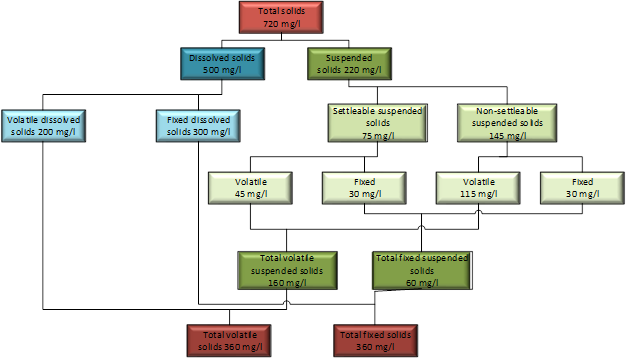
\includegraphics[scale=0.8]{WastewaterSolids}\\
					\caption{Typical Wastewater Solids Concentrations}
				\end{center}
				\end{figure}
% % 			\end{enumerate}
				
\section{Nutrients}\index{Nutrients}	
% 			\begin{snugshade*}
% 				\item \noindent\textsc{Nutrients}
% 			\end{snugshade*}	
			\begin{itemize}
				\item Plant nutrients - nitrogen and phosphorous, present in wastewater effluent discharge, promote growth of plant and algal matter in the receiving waters causing destruction of the normal aquatic life mainly due to oxygen depletion - eutrophication.
				      
				\item Because of the potential impacts of the presence of these nutrients in wastewater effluent on the receiving waters,  limits on the levels of these nutrients is typically stipulated in the treatment plant's wastewater discharge permit.
				      
				\item Typically, conventional secondary treatment processes are designed primarily remove the organics from the wastewater.  Secondary treatment process designed to additionally remove nutrients is deemed as tertiary or advanced treatment is termed as Biological Nutrient Removal (BNR).
			\end{itemize}
	\subsection{Nitrogen}\index{Nitrogen}				
% 			\begin{enumerate}%@@@@@@@@@@@@@@@@@@%
% 				\definecolor{shadecolor}{RGB}{220,220,220}
% 				\begin{snugshade*}
% 					\item \noindent\textsc{Nitrogen}%@@@@@@@@@@@@@@@@@@%
% 				\end{snugshade*}

	\subsubsection{Forms of nitrogen}\index{Forms of nitrogen}	
% 				\begin{itemize}
% 					\item Forms of nitrogen:\\
					      \begin{itemize}
					      	\item About 60\% of nitrogen in wastewater is present as ammonia nitrogen (about 60\%).  The ammonium nitrogen is present either in the form of ammonia (NH$_3$ ) or as ammonium (NH$_4^+$ ) ion.   These two forms can rapidly change from one to the other depending on pH and temperature.  Under low pH (acidic) or neutral conditions – pH less than or equal to 7, ammonia exists mostly as ammonium.  Ammonia becomes the dominant form as the pH increases to 8 and beyond.
					      	\item The other dominant form of nitrogen, about 40\% of the total nitrogen is as organic nitrogen
					      	\item Nitrogen measured as Total Kjeldahl Nitrogen (TKN) which is the sum of the organic nitrogen and the ammonia nitrogen concentrations.  Total inorganic nitrogen is the total concentration of ammonia nitrogen, NO3-, and NO2-.   Table provides the concentrations and forms of nitrogen in wastewater.
					      \end{itemize}
					      \setlength{\arrayrulewidth}{0.7mm}
					      \setlength{\tabcolsep}{8 pt}
					      \renewcommand{\arraystretch}{0.8}
					      \begin{center}
					      \begin{figure}[!htbp]
					      	\noindent \begin{tabular}[!htbp]{ |p{6cm}|p{2.0cm}|p{2.5cm}|p{2.cm}|}
					      	\hline
					      	\multicolumn{4}{|c|}{\textbf{Forms of Nitrogen in Wastewater}} \\
					      	\hline
					      	%\thead{A Head} & \thead{A Second \\ Head} & \thead{A Third \\ Head} \\
					      	%\hline%
					      	
					      	\hspace{1.8 cm}Forms of Nitrogen & \hspace{0.25 cm} Formula & \hspace{.4 cm} Found in & \hspace{.4 cm} Typical \newline \hspace{.2 cm}Concentration\\
					      	\hline
					      	\small Ammonia/Ammonium & \small NH$_3$/NH$_4^{\enspace +}$ &  \small Influent wastewater & 30-50 mg/l\\
					      	
					      	Total Kjeldahl Nitrogen \newline  \small (Ammonia/Ammonium + Organic Nitrogen) &  \small TKN &  \small Wastewater \newline  \small effluent  & 30-60 mg/l \\
					      	
					      	\small Total Inorganic Nitrogen \newline  \small (Ammonia/Ammonium + Nitrite + Nitrate) & \small TIN &  \small  Wastewater \newline  \small effluent  & 1-40 mg/l \\
					      	
					      	\small Nitrate  & $NO_3^{\enspace -}$ &  \small Nitrified effluent &  \small 1-35 mg/l \\
					      	
					      	\small Nitrate  &  $NO_2^{\enspace -}$ &  \small Partially nitrified effluent &  \small 0.1-2 mg/l \\
					      	
					      	\hline
					      	\end{tabular}
					      	\caption{Forms of Nitrogen}
					      	\end{figure}
					      \end{center}
					      
		\subsection{Phosphorous}\index{Phosphorous}			
		\subsubsection{Forms of phosphorous}\index{Forms of phosphorous}
					      \begin{itemize}
					      	\item The principal forms are organically bound phosphorus, polyphosphates, and orthophosphates.
					      	\item Organically bound phosphorus originates from body and food waste and, upon biological decomposition of these solids, is converted to orthophosphates. 
					      	\item Polyphosphates originate from synthetic detergents and are hydrolyzed to orthophosphates. Thus, the principal form of phosphorus in wastewater is assumed to be orthophosphates, although the other forms may exist. Orthophosphates consist of the negative ions PO$_4$$^{3-}$, HPO$_4$$^{2-}$, and H$_2$PO$_4$ $^-$.  These may form chemical combinations with cations (positively charged ions).
					      \end{itemize}

\section{Oil and Grease}\index{Oil and Grease}	
			Fats, oil and grease in wastewater originate from homes, food establishments and industries.
			\begin{itemize}
				\item Oil and grease content of wastewater is established in the laboratory by extracting it with a solvent - \textit{n}-hexane.  The concentration of oil and grease is reported in mg/l and typical oil and grease content of wastewater ranges from 80 - 120 mg/l
				\item Presence of excessive oils and grease could potentially impact the secondary treatment process
				\item Oils and grease are removed as floatables in primary treatment and sent with the sludge to the digesters
			\end{itemize}
		



\section{Wastewater Parameters}\index{Wastewater Parameters}			
		Laboratory and field tests are conducted to measure parameters which are critical for monitoring and controlling treatment.  The following are the key parameters that are measured.	
			
\subsection{pH}\index{pH}	
			\hl{pH is a measure of the hydrogen ion (H$^+$) content or the acidity or basicity of a solution.}  pH impacts the chemical and micribiological elements of wastewater treatment processes and thus pH measurement and control is critical.
			\begin{itemize}
				\item Pure water dissociates into equal concentration of hydrogen ions and hydroxide ions:\\ 
				      $H_2O \rightarrow H^+ + OH^-$.
				\item The H$^+$ are responsible for acidic properties and the OH$^-$ ions for the basic properties.  
				\item pH is the inverse of H$^+$ concentration; pH increases when the concentration of H$^+$ decreases relative to the concentration of OH-. 
				\item pH scale ranges from 0 – 14. When the concentration of both H$^+$ and OH$^-$ are equal, as in pure water, it is considered neutral and its pH is 7.0.  \item If the pH of a sample solution is below 7.0, the sample is termed acidic and is alkaline or basic if its pH is above 7.0. 
				\item Each change of 1 pH unit represents a 10 fold change in concentration.  For example, a sample with a pH of 2.0 is 1000 times more acidic than a sample with a pH of 5.0. 
				\item pH is measured by an electrode that is sensitive only to H$^+$ or using a pH strip which is essentially an adsorbent paper which is pre-impregnated with chemicals which change color under different H$^+$ concentrations.
				\item Most organisms involved in biological wastewater treatment processes do well within a a narrow range of pH near neutral (pH of 7).			
			\end{itemize}
			
\subsection{Oxidation Reduction Potential (ORP)}\index{Oxidation Reduction Potential (ORP)}			
			ORP is a measure of the potential of a wastewater to allow for microbiological oxidation and reduction reactions.\\
			An example of wastewater treatment process where microbiological oxidation involved include the activated sludge process.  Whereas, anaerobic digestion is a microbiological reduction based process.
			\begin{itemize}
				\item ORP value is measured in millivolts (mV), using an electrochemical probe
				\item The measured ORP value provides an indication of the potential of oxidation and reduction reactions in that sample.
				\item A higher positive ORP is indicative of oxidation potential of the wastewater whereas a negative ORP value indicates potential for a reduction reaction to occur.
				\item ORP measurements are used for controlling treatment processes including nitrification, odor control and disinfection.  For example, in the disinfection process utilizing chlorine (bleach), ORP measurements provides the strength of the oxidation potential of chlorine present in the wastewater being disinfected.  This measurement is used for precisely controlling the chlorine dosing.  The proper chlorine control results in optimizing chlorine dosing which reduces potential toxicity issues and dechlorination costs.
			\end{itemize}
			Typical ORP applications include the following processes and process elements
			
			
			\setlength{\arrayrulewidth}{0.3mm}
			\setlength{\tabcolsep}{8 pt}
			\renewcommand{\arraystretch}{0.8}
			\begin{center}
				\begin{tabular}{ |p{9.5cm}|p{4.0cm}|}
					\hline
					\multicolumn{2}{|c|}{\textbf{Typical Wastewater Process ORPs}} \\
					\hline
					
					\hline
					\small Collections	Sulfide formation                                & \small -50 to -250 mV  \\
					\small Influent wastewater                                          & \small - 200 mV        \\
					\small Activated sludge	cBOD degradation with free molecular oxygen & \small +50 to +250 mV  \\
					\small Biological phosphorous removal                               & \small +25 to +250 mV  \\
					\small Denitrification                                              & \small +50 to -50 mV   \\
					\small Anaerobic Digestion: Acid formation (Acidogenesis)           & \small -100 to -225 mV \\
					\small Anaerobic Digestion: Methane production (Methanogenesis)     & \small -75 to -400 mV  \\
					\hline
				\end{tabular}
				
			\end{center}
			
\subsection{Alkalinity}\index{Alkalinity}	
			\begin{itemize}
				\item \hl{Alkalinity is the ability of a water to neutralize acids.}  
				\item During certain wastewater treatment processes including anaerobic digestion, acids are generated as a result of microbiological activity.  The bacteria and other biological entities which play an active role in wastewater treatment are most effective at a neutral to slightly alkaline pH of 7 to 8.  In order to maintain these optimal pH conditions for biological activity there must be sufficient alkalinity present in the wastewater to neutralize acids generated by the active biomass.
				\item This ability to maintain the proper pH in the wastewater as it undergoes treatment is the reason why alkalinity is so important to the wastewater industry.
				\item The alkalinity is due to the presence of acid neutralizing bases in the water including the hydroxyl (OH$^-$), carbonate (CO$_3$$^-$) and bicarbonate (HCO$_3$$^-$)  ions.  These ions are of mineral origin and are also formed from carbon dioxide which comes from the atmosphere and from the microbial decomposition of organic material.  The resistance to pH change of the water will continue until all the alkalinity contributing ions are neutralized.  
				\item The pH of a water serves as a guide to the types of alkalinity present in the water but is unrelated to the alkalinity content of a water.  Important Note:  Alkalinity is a measure of the ability to neutralize acids whereas a solution is termed alkaline (or basic) if its pH greater than 7. 
				\item Alkalinity is expressed as milligrams per liter of CaCO$_3$
			\end{itemize}
			
\subsection{Dissolved Oxygen}\index{Dissolved Oxygen}	
			\begin{itemize}
				\item Dissolved oxygen (DO) is the concentration of oxygen dissolved in the wastewater sample and is typically measured in the field using a DO probe.  A titration based Winkler Test is used in the laboratory
				\item The \hl{presence of oxygen indicates an aerobic environment} where dissolved, free oxygen is available for aerobic microorganisms to live, BOD removal in the activated sludge process occurs as a result of the activity of aerobic bacteria.  The absence of DO indicates that the environment or condition is either anoxic or anaerobic.  
				\item \hl{In an anoxic environment, free oxygen is not present, but oxygen is available from its combined  forms - nitrate (NO$_3$ $^-$) and sulfate (SO$_4$ $^-$)} for the the consumption of microorganisms.  Example of an anoxic process is denitrification.  In denitrification, the anoxic bacteria in the presence of food (cBOD) consume the combined oxygen in nitrates (NO$_3$ $^-$ ) and convert it to nitrogen gas.
				\item \hl{The complete absence of oxygen including free and combined oxygen is an anaerobic environment.}
				\item Microorganisms are termed as obligate aerobes if they cannot survive without free oxygen.  Facultative aerobes are microorganisms which can survive in both aerobic and anaerobic environments.  
			\end{itemize}
			
\subsection{Microbiological testing and monitoring}\index{Microbiological testing and monitoring}	
			
			Microbiological testing and monitoring is conducted as part of the wastewater treatment for two main reasons:
			\begin{enumerate}[1.]
				\item Heterotrohic (organisms that consume organic material) microbes are responsible for the biological wastewater treatment processes - secondary treatment process, digestion and nutrient removal; and
				\item Pathogens - agents that cause disease are present in wastewater effluent.
			\end{enumerate}

\begin{itemize}
				
				\item Microbiological testing related to monitoring and troubleshooting biological wastewater treatment\\
				
				Microbes involved in biological wastewater treatment processes include:\\
				\begin{itemize}
					\item Fungi - Filamentous fungi occasionally bloom in activated sludge processes due to low pH or nutrient deficiency and cause problems with the settleability.
					\item Protozoa - Protozoas play a important role in the secondary treatment process.  Common protozoas in the activated sludge process include:
					      \begin{itemize}
					      	\item Amoeba
					      	\item Flagellate
					      	\item Cilliate
					      \end{itemize}
					\item Rotifers
					\item Nematodes
					\item Bacteria - Bacteria is the predominant microorganism responsible for the biological wastewater water treatment.  
				\end{itemize}
				\begin{itemize}
					\item The effectiveness of the biological wastewater treatment processes is primarily due to the presence of a microbial ecosystem with a right balance of populations of different microbial species.
					\item Methods used for monitoring the microbial composition include direct monitoring using a light microscope to see which and how many of the different microbial species are present - typically used for activated sludge process.
					\item Indirect method includes monitoring other parameters such as pH and alkalinity which are influenced by microbiological activity.
					\item The microbial monitoring ensures process stability and helps identify potential process upset conditions caused by changes to the microbial population due to other external factors - toxicty, organic loading, temperature etc.
				\end{itemize}

\item Microbiological testing related to monitoring and controlling pathogens in treated wastewater effluent\\

	
				Pathogens in wastewater belong to the following groups:
				\begin{itemize}
					\item Bacteria:  Although, bacteria is present in large numbers in feces, pathogenic or bacteria are present only because of an infection and this pathogenic bacteria can potentially spread the infection to other healthy individuals.  Disease spread by pathogenic bacteria include diarrhea, cholera and typhoid among many others.
					      
					\item Viruses: A large number of viruses may infect humans and are present in feces.  These include enteroviruses (including polioviruses), hepatitis A virus, reoviruses and diarrhea-causing viruses (especially rotavirus).
					      
					\item Protozoa:  Many species of protozoa can infect humans and cause diarrhoea and dysentery. Girardia which casues diarrheal illness is an example of a protozoan pathogen
					      
					\item Helminths:  These are parasitic worms that can infect humans and are transmitted to others through its eggs or larval forms
					      
				\end{itemize}
				
				\begin{itemize}
					\item As one of the main reasons for treating wastewater is to protect public health, microbiological/pathogen testing of the wastewater effluent and the surface water impacted by the wastewater discharge is conducted to meet the requirements of a wastewater discharge permit, to monitor the pathogen impact of treated wastewater discharge and assess the level of contamination of a public body of water.
					\item The bacteriological tests involves detection and quantification of one or more of the following bacteria:  total coliforms, fecal coliforms, E. Coli, and Enterococcus.  
					      \begin{itemize}
					      	\item The main reason why these bacteria such as coliforms and enterococcus are used \hl{as it is not practical to detect and quantify all pathogens associated with wastewater.}  
					      	\item These selected bacteria originate from feces and indicate fecal contamination and thus serve as an indicator organisms for pathogens of wastewater origin.  
					      	\item Also, they are abundant, potentially less harmful, and easy to detect.  E. coli has been shown to be a better predictor of the potential for impacts to human health and therefore many newer wastewater discharge permits require E. Coli testing in lieu of fecal coliform testing requirements.
					      \end{itemize}
					\item The microbiological test sample is always collected as a grab in a clean, sterile borosilicate glass or plastic bottle containing sodium thiosulfate. 
					      \begin{itemize}
					      	\item Sodium thiosulfate is added to remove residual chlorine which will kill coliforms during transit. 
					      	\item If the sample is not preserved or maintained under proper conditions until the test is conducted in the laboratory, the test would provide erroneous results.
					      	\item Samples must be refrigerated if they cannot be analyzed within 1 hour of collection and must be handled with care to prevent contamination and adverse conditions such as prolonged exposure to direct sunlight.
					      	\item The maximum holding time for state or federal permit reporting purposes is 6 hours. 
					      \end{itemize} 
					\item As it is not possible to exactly quantify the number of bacteria present, a statistical based - \hl{Most Probable Number (MPN)} approach is utilized.  The methods for wastewater bacteriological tests include:  multiple-tube fermentation technique, membrane filtration and quanti-tray testing. 
				\end{itemize}
			\end{itemize}

\subsection{Specific Gravity}\index{Specific Gravity}				
			\begin{itemize}
				\item Specific gravity is a term to express the weight of a solution with respect to that of water
				\item Water weighs 1 kg/L or 8.34 lbs/gallon or 62.4 lbs/ft$^3$
				\item A solution with a specific gravity of 1.2 will weigh 1.2 times the same volume of water.  1 L of that solution will weigh ( 1.2 kg )/L  or  ( 1.2*8.34=10lbs )/gallon.
				\item Typically wastewater and the associated unthickened sludge, for all practical purposes is assumed to have a specific gravity of 1 - implying 8.34 lbs/gallon.
				\item Specific gravity is typically used for calculations related to chemicals used in wastewater treatment.
			\end{itemize}
			
\section{Wastewater Sampling}\index{Wastewater Sampling}
		\begin{itemize}
			\item Field or laboratory measurement of a certain parameter is critical in wastewater treatment operations to obtain information about wastewater characteristics in order to either characterize a wastewater stream, or to monitor a treatment process or for permit compliance.  
			\item A sample is a small part of the whole representing the whole.  Thus, a sample needs to be such that it truly represents the entire population – which in a wastewater operations could be either a wastewater stream, wastewater solids or a chemical used.
		\end{itemize}
		
\subsection{Sampling Methods}\index{Sampling Methods}
\subsubsection{Grab Samples}\index{Grab Samples}
				\begin{itemize}
					\item A grab sample is a sample collected at a specific spot at a site over a short period of time.  
					\item Grab sampling allows for instantaneous analysis of parameters such as pH, dissolved oxygen, chlorine residual, temperature and other parameters which change rapidly with time.
					\item A grab sample represents a snapshot of space and time of a process stream.
					\end{itemize}
\subsubsection{Composite Samples}\index{Composite Samples}
				\begin{itemize}
					\item A composite sample is a collection of discrete samples are combined over a certain period or space and therefore represent the average performance of a wastewater treatment plant or a process during the collection period.\\  
					\item Composite sampling can be either based on:
					      
					      1. constant time interval (time proportioned sampling)\\
					      2. constant wastewater volume interval (flow-proportioned sampling), and\\
					      3. treatment process space - includes samples taken at different depths\\
					      
					\item Composite samples are typically collected using automated samplers which can be programmed to collect samples at pre-established time intervals – for time proportional sampling.
					\item Time and space composite samples are collected by adding equal volumes of samples collected from different times or locations.  
					\item Flow proportional composite samples comprise of volume of each subsample based on flow.\\  
				\end{itemize}
				
			\begin{center}
				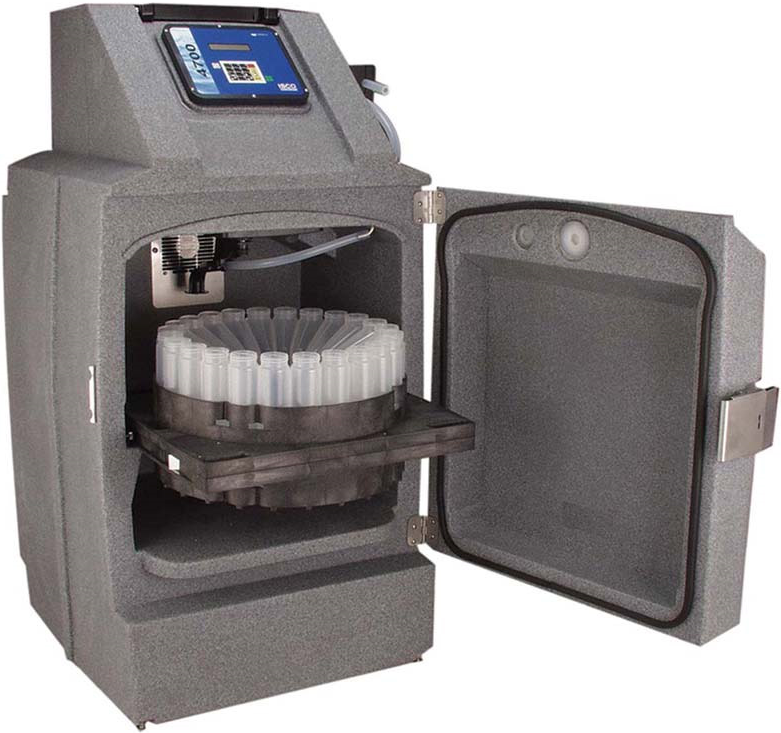
\includegraphics[scale=0.2]{Autosampler} \hspace{2cm} 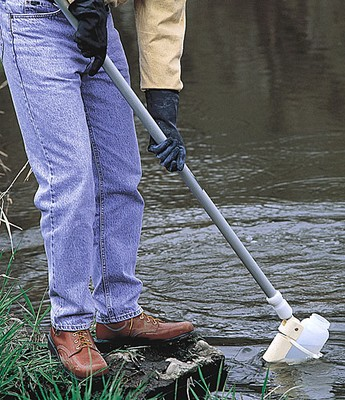
\includegraphics[scale=0.37]{Grabsampler}\\
			\end{center}
			\hspace{2.3cm} Automated Sampler \hspace{2.0cm} \parbox{\textwidth}{Grab Sampling Using a Long Handle Dipper}\\

\subsubsection{Sampling Precautions and Protocols}\index{Sampling Precautions and Protocols}
			\begin{itemize}
				\item Samples should represent the major portion of the process or the process stream and should be taken from places where the mixing is thorough, avoiding dead spots and areas of heavier or lighter loadings. 
				\item The collected sample is invariably exposed to conditions very different from the original source and is subject to change due to chemical and microbiological activity.  
				\item Thus, in order to ensure integrity of sample, sample preservation techniques specific to the analysis to be performed is needed.  
				      \begin{itemize}
				      	\item The preservation technique should not only allow for stabilizing the parameter to be analyzed, it should also not interfere with the analyses.  
				      	\item The common preservation techniques involve use of proper containers, temperature control, addition of chemical preservatives, and observance of the recommended maximum sample holding time.
				      \end{itemize}
			\end{itemize}

\section{Data Reporting}\index{Data Reporting}	
		\begin{itemize}
			\item Arithmetic mean is typically calculated for reporting data where multiple samples have been collected and analyzed for the same process stream at different times and for reporting average value over a certain time period – daily, monthly etc.\\ \item Arithmetic mean mathematically is calculated by adding all the result values and dividing by the total number of data points.\\
		\end{itemize}
		Mathematically the arithmetic mean is represented as:\\
		$$\bar{x}=\dfrac{\sum_{i=1}^{n} x^i}{n} = \dfrac{x_1+x_2+x_3...x_n}{n}$$
		For example:\\
		Arithmetic mean of the following set of data points:  200, 304, 250, 400 is calculated as:\\
		\vspace{10pt}
		Arithmetic Mean = $\dfrac{200 + 302 + 250 + 400}{4}= 288$\\
		\vspace{10pt}
		For data sets for analysis such as fecal coliform could include values which vary by several orders of magnitudes, using the arithmetic mean to report the average value is not appropriate as the lower or higher values would bias the calculated mean.\\
		\vspace{10pt}
		For example, consider a data set with values:  260, 300, 500, 5,000, 320 and 200.\\
		\vspace{10pt}
		The arithmetic mean = $\dfrac{260+300+500+5,000+320+200}{6} = 3,444$\\
		Here the 5000 value completely skews the arithmetic mean.
		
		Therefore, for such tests, the geometric mean calculation is used for reporting the average value.\\
		
		
		Mathematically a geometric mean is represented as:\\
		$$\Bigg(\prod_{i=a}^n\Bigg)^{\dfrac{1}{n}}=\sqrt[n]{a_1*a_2*a_3...a_n}$$
		 
		Calculation method:\\
		1.	Find the product of all the data points (analogous to first calculating the sum of all the data points when calculating the arithmetic mean)\\
		260*300*500*5,000*320*200 = 12,480,000,000,000,000\\
		2.	Raise the product to the inverse of the number of data points\\
		(*Using the power function of a scientific calculator)\\
		Here n (\# data points) = 6 $\implies$ geometric mean = $(12,480,000,000,000,000)^{\dfrac{1}{6}}   = 482$

\end{document}
%% This is an example of theorems.
%\part{Module 7}
%\input{WATR080 Module7.tex}
% \subsection{Several equations}\index{Theorems!Several Equations}
% This is a theorem consisting of several equations.

% \begin{theorem}[Name of the theorem]
% In $E=\mathbb{R}^n$ all norms are equivalent. It has the properties:
% \begin{align}
% & \big| ||\mathbf{x}|| - ||\mathbf{y}|| \big|\leq || \mathbf{x}- \mathbf{y}||\\
% &  ||\sum_{i=1}^n\mathbf{x}_i||\leq \sum_{i=1}^n||\mathbf{x}_i||\quad\text{where $n$ is a finite integer}
% \end{align}
% \end{theorem}

% \subsection{Single Line}\index{Theorems!Single Line}
% This is a theorem consisting of just one line.

% \begin{theorem}
% A set $\mathcal{D}(G)$ in dense in $L^2(G)$, $|\cdot|_0$. 
% \end{theorem}

% %------------------------------------------------

% \section{Definitions}\index{Definitions}

% This is an example of a definition. A definition could be mathematical or it could define a concept.

% \begin{definition}[Definition name]
% Given a vector space $E$, a norm on $E$ is an application, denoted $||\cdot||$, $E$ in $\mathbb{R}^+=[0,+\infty[$ such that:
% \begin{align}
% & ||\mathbf{x}||=0\ \Rightarrow\ \mathbf{x}=\mathbf{0}\\
% & ||\lambda \mathbf{x}||=|\lambda|\cdot ||\mathbf{x}||\\
% & ||\mathbf{x}+\mathbf{y}||\leq ||\mathbf{x}||+||\mathbf{y}||
% \end{align}
% \end{definition}

% %------------------------------------------------

% \section{Notations}\index{Notations}

% \begin{notation}
% Given an open subset $G$ of $\mathbb{R}^n$, the set of functions $\varphi$ are:
% \begin{enumerate}
% \item Bounded support $G$;
% \item Infinitely differentiable;
% \end{enumerate}
% a vector space is denoted by $\mathcal{D}(G)$. 
% \end{notation}

%------------------------------------------------

% \section{Remarks}\index{Remarks}

% This is an example of a remark.

% \begin{remark}
% The concepts presented here are now in conventional employment in mathematics. Vector spaces are taken over the field $\mathbb{K}=\mathbb{R}$, however, established properties are easily extended to $\mathbb{K}=\mathbb{C}$.
% \end{remark}

% %------------------------------------------------

% \section{Corollaries}\index{Corollaries}

% This is an example of a corollary.

% \begin{corollary}[Corollary name]
% The concepts presented here are now in conventional employment in mathematics. Vector spaces are taken over the field $\mathbb{K}=\mathbb{R}$, however, established properties are easily extended to $\mathbb{K}=\mathbb{C}$.
% \end{corollary}

%------------------------------------------------

% \section{Propositions}\index{Propositions}

% This is an example of propositions.

% \subsection{Several equations}\index{Propositions!Several Equations}

% \begin{proposition}[Proposition name]
% It has the properties:
% \begin{align}
% & \big| ||\mathbf{x}|| - ||\mathbf{y}|| \big|\leq || \mathbf{x}- \mathbf{y}||\\
% &  ||\sum_{i=1}^n\mathbf{x}_i||\leq \sum_{i=1}^n||\mathbf{x}_i||\quad\text{where $n$ is a finite integer}
% \end{align}
% \end{proposition}

% \subsection{Single Line}\index{Propositions!Single Line}

% \begin{proposition} 
% Let $f,g\in L^2(G)$; if $\forall \varphi\in\mathcal{D}(G)$, $(f,\varphi)_0=(g,\varphi)_0$ then $f = g$. 
% \end{proposition}

%------------------------------------------------

% \section{Examples}\index{Examples}

% This is an example of examples.

% \subsection{Equation and Text}\index{Examples!Equation and Text}

% \begin{example}
% Let $G=\{x\in\mathbb{R}^2:|x|<3\}$ and denoted by: $x^0=(1,1)$; consider the function:
% \begin{equation}
% f(x)=\left\{\begin{aligned} & \mathrm{e}^{|x|} & & \text{si $|x-x^0|\leq 1/2$}\\
% & 0 & & \text{si $|x-x^0|> 1/2$}\end{aligned}\right.
% \end{equation}
% The function $f$ has bounded support, we can take $A=\{x\in\mathbb{R}^2:|x-x^0|\leq 1/2+\epsilon\}$ for all $\epsilon\in\intoo{0}{5/2-\sqrt{2}}$.
% \end{example}

% \subsection{Paragraph of Text}\index{Examples!Paragraph of Text}

% \begin{example}[Example name]
% \lipsum[2]
% \end{example}

%------------------------------------------------

% \section{Exercises}\index{Exercises}

% This is an example of an exercise.

% \begin{exercise}
% This is a good place to ask a question to test learning progress or further cement ideas into students' minds.
% \end{exercise}

%------------------------------------------------

% \section{Problems}\index{Problems}

% \begin{problem}
% What is the average airspeed velocity of an unladen swallow?
% \end{problem}

%------------------------------------------------

% \section{Vocabulary}\index{Vocabulary}

% Define a word to improve a students' vocabulary.

% \begin{vocabulary}[Word]
% Definition of word.
% \end{vocabulary}

%----------------------------------------------------------------------------------------
%	PART 3
%----------------------------------------------------------------------------------------

%\part{Analysis and Testing}

%----------------------------------------------------------------------------------------
%	CHAPTER 3
%----------------------------------------------------------------------------------------
%\input{WastewaterAnalysisandLaboratoryMethods.tex}
% \chapterimage{chapter_head_1.pdf} % Chapter heading image

% \chapter{Presenting Information}

% \section{Table}\index{Table}

% \begin{table}[h]
% \centering
% \begin{tabular}{l l l}
% \toprule
% \textbf{Treatments} & \textbf{Response 1} & \textbf{Response 2}\\
% \midrule
% Treatment 1 & 0.0003262 & 0.562 \\
% Treatment 2 & 0.0015681 & 0.910 \\
% Treatment 3 & 0.0009271 & 0.296 \\
% \bottomrule
% \end{tabular}
% \caption{Table caption}
% \label{tab:example} % Unique label used for referencing the table in-text
% %\addcontentsline{toc}{table}{Table \ref{tab:example}} % Uncomment to add the table to the table of contents
% \end{table}

% Referencing Table \ref{tab:example} in-text automatically.

% %------------------------------------------------

% \section{Figure}\index{Figure}

% \begin{figure}[h]
% \centering
\includegraphics[scale=0.5]{placeholder.jpg}
% \caption{Figure caption}
% \label{fig:placeholder} % Unique label used for referencing the figure in-text
% %\addcontentsline{toc}{figure}{Figure \ref{fig:placeholder}} % Uncomment to add the figure to the table of contents
% \end{figure}

% Referencing Figure \ref{fig:placeholder} in-text automatically.

%----------------------------------------------------------------------------------------
%%	BIBLIOGRAPHY
%%----------------------------------------------------------------------------------------
%
%\chapter*{Bibliography}
%\addcontentsline{toc}{chapter}{\textcolor{ocre}{Bibliography}} % Add a Bibliography heading to the table of contents
%
%%------------------------------------------------
%
%\section*{Articles}
%\addcontentsline{toc}{section}{Articles}
%\printbibliography[heading=bibempty,type=article]
%
%%------------------------------------------------
%
%\section*{Books}
%\addcontentsline{toc}{section}{Books}
%\printbibliography[heading=bibempty,type=book]
%
%%----------------------------------------------------------------------------------------
%%	INDEX
%%----------------------------------------------------------------------------------------
%
%\cleardoublepage % Make sure the index starts on an odd (right side) page
%\phantomsection
%\setlength{\columnsep}{0.75cm} % Space between the 2 columns of the index
%\addcontentsline{toc}{chapter}{\textcolor{ocre}{Index}} % Add an Index heading to the table of contents
%\printindex % Output the index

%----------------------------------------------------------------------------------------

\end{document}
